% Options for packages loaded elsewhere
\PassOptionsToPackage{unicode}{hyperref}
\PassOptionsToPackage{hyphens}{url}
\PassOptionsToPackage{dvipsnames,svgnames,x11names}{xcolor}
%
\documentclass[
  letterpaper,
  DIV=11,
  numbers=noendperiod,
  oneside]{scrreprt}

\usepackage{amsmath,amssymb}
\usepackage{iftex}
\ifPDFTeX
  \usepackage[T1]{fontenc}
  \usepackage[utf8]{inputenc}
  \usepackage{textcomp} % provide euro and other symbols
\else % if luatex or xetex
  \usepackage{unicode-math}
  \defaultfontfeatures{Scale=MatchLowercase}
  \defaultfontfeatures[\rmfamily]{Ligatures=TeX,Scale=1}
\fi
\usepackage{lmodern}
\ifPDFTeX\else  
    % xetex/luatex font selection
\fi
% Use upquote if available, for straight quotes in verbatim environments
\IfFileExists{upquote.sty}{\usepackage{upquote}}{}
\IfFileExists{microtype.sty}{% use microtype if available
  \usepackage[]{microtype}
  \UseMicrotypeSet[protrusion]{basicmath} % disable protrusion for tt fonts
}{}
\makeatletter
\@ifundefined{KOMAClassName}{% if non-KOMA class
  \IfFileExists{parskip.sty}{%
    \usepackage{parskip}
  }{% else
    \setlength{\parindent}{0pt}
    \setlength{\parskip}{6pt plus 2pt minus 1pt}}
}{% if KOMA class
  \KOMAoptions{parskip=half}}
\makeatother
\usepackage{xcolor}
\usepackage[left=1in,marginparwidth=2.0666666666667in,textwidth=4.1333333333333in,marginparsep=0.3in]{geometry}
\setlength{\emergencystretch}{3em} % prevent overfull lines
\setcounter{secnumdepth}{5}
% Make \paragraph and \subparagraph free-standing
\makeatletter
\ifx\paragraph\undefined\else
  \let\oldparagraph\paragraph
  \renewcommand{\paragraph}{
    \@ifstar
      \xxxParagraphStar
      \xxxParagraphNoStar
  }
  \newcommand{\xxxParagraphStar}[1]{\oldparagraph*{#1}\mbox{}}
  \newcommand{\xxxParagraphNoStar}[1]{\oldparagraph{#1}\mbox{}}
\fi
\ifx\subparagraph\undefined\else
  \let\oldsubparagraph\subparagraph
  \renewcommand{\subparagraph}{
    \@ifstar
      \xxxSubParagraphStar
      \xxxSubParagraphNoStar
  }
  \newcommand{\xxxSubParagraphStar}[1]{\oldsubparagraph*{#1}\mbox{}}
  \newcommand{\xxxSubParagraphNoStar}[1]{\oldsubparagraph{#1}\mbox{}}
\fi
\makeatother

\usepackage{color}
\usepackage{fancyvrb}
\newcommand{\VerbBar}{|}
\newcommand{\VERB}{\Verb[commandchars=\\\{\}]}
\DefineVerbatimEnvironment{Highlighting}{Verbatim}{commandchars=\\\{\}}
% Add ',fontsize=\small' for more characters per line
\usepackage{framed}
\definecolor{shadecolor}{RGB}{241,243,245}
\newenvironment{Shaded}{\begin{snugshade}}{\end{snugshade}}
\newcommand{\AlertTok}[1]{\textcolor[rgb]{0.68,0.00,0.00}{#1}}
\newcommand{\AnnotationTok}[1]{\textcolor[rgb]{0.37,0.37,0.37}{#1}}
\newcommand{\AttributeTok}[1]{\textcolor[rgb]{0.40,0.45,0.13}{#1}}
\newcommand{\BaseNTok}[1]{\textcolor[rgb]{0.68,0.00,0.00}{#1}}
\newcommand{\BuiltInTok}[1]{\textcolor[rgb]{0.00,0.23,0.31}{#1}}
\newcommand{\CharTok}[1]{\textcolor[rgb]{0.13,0.47,0.30}{#1}}
\newcommand{\CommentTok}[1]{\textcolor[rgb]{0.37,0.37,0.37}{#1}}
\newcommand{\CommentVarTok}[1]{\textcolor[rgb]{0.37,0.37,0.37}{\textit{#1}}}
\newcommand{\ConstantTok}[1]{\textcolor[rgb]{0.56,0.35,0.01}{#1}}
\newcommand{\ControlFlowTok}[1]{\textcolor[rgb]{0.00,0.23,0.31}{\textbf{#1}}}
\newcommand{\DataTypeTok}[1]{\textcolor[rgb]{0.68,0.00,0.00}{#1}}
\newcommand{\DecValTok}[1]{\textcolor[rgb]{0.68,0.00,0.00}{#1}}
\newcommand{\DocumentationTok}[1]{\textcolor[rgb]{0.37,0.37,0.37}{\textit{#1}}}
\newcommand{\ErrorTok}[1]{\textcolor[rgb]{0.68,0.00,0.00}{#1}}
\newcommand{\ExtensionTok}[1]{\textcolor[rgb]{0.00,0.23,0.31}{#1}}
\newcommand{\FloatTok}[1]{\textcolor[rgb]{0.68,0.00,0.00}{#1}}
\newcommand{\FunctionTok}[1]{\textcolor[rgb]{0.28,0.35,0.67}{#1}}
\newcommand{\ImportTok}[1]{\textcolor[rgb]{0.00,0.46,0.62}{#1}}
\newcommand{\InformationTok}[1]{\textcolor[rgb]{0.37,0.37,0.37}{#1}}
\newcommand{\KeywordTok}[1]{\textcolor[rgb]{0.00,0.23,0.31}{\textbf{#1}}}
\newcommand{\NormalTok}[1]{\textcolor[rgb]{0.00,0.23,0.31}{#1}}
\newcommand{\OperatorTok}[1]{\textcolor[rgb]{0.37,0.37,0.37}{#1}}
\newcommand{\OtherTok}[1]{\textcolor[rgb]{0.00,0.23,0.31}{#1}}
\newcommand{\PreprocessorTok}[1]{\textcolor[rgb]{0.68,0.00,0.00}{#1}}
\newcommand{\RegionMarkerTok}[1]{\textcolor[rgb]{0.00,0.23,0.31}{#1}}
\newcommand{\SpecialCharTok}[1]{\textcolor[rgb]{0.37,0.37,0.37}{#1}}
\newcommand{\SpecialStringTok}[1]{\textcolor[rgb]{0.13,0.47,0.30}{#1}}
\newcommand{\StringTok}[1]{\textcolor[rgb]{0.13,0.47,0.30}{#1}}
\newcommand{\VariableTok}[1]{\textcolor[rgb]{0.07,0.07,0.07}{#1}}
\newcommand{\VerbatimStringTok}[1]{\textcolor[rgb]{0.13,0.47,0.30}{#1}}
\newcommand{\WarningTok}[1]{\textcolor[rgb]{0.37,0.37,0.37}{\textit{#1}}}

\providecommand{\tightlist}{%
  \setlength{\itemsep}{0pt}\setlength{\parskip}{0pt}}\usepackage{longtable,booktabs,array}
\usepackage{calc} % for calculating minipage widths
% Correct order of tables after \paragraph or \subparagraph
\usepackage{etoolbox}
\makeatletter
\patchcmd\longtable{\par}{\if@noskipsec\mbox{}\fi\par}{}{}
\makeatother
% Allow footnotes in longtable head/foot
\IfFileExists{footnotehyper.sty}{\usepackage{footnotehyper}}{\usepackage{footnote}}
\makesavenoteenv{longtable}
\usepackage{graphicx}
\makeatletter
\newsavebox\pandoc@box
\newcommand*\pandocbounded[1]{% scales image to fit in text height/width
  \sbox\pandoc@box{#1}%
  \Gscale@div\@tempa{\textheight}{\dimexpr\ht\pandoc@box+\dp\pandoc@box\relax}%
  \Gscale@div\@tempb{\linewidth}{\wd\pandoc@box}%
  \ifdim\@tempb\p@<\@tempa\p@\let\@tempa\@tempb\fi% select the smaller of both
  \ifdim\@tempa\p@<\p@\scalebox{\@tempa}{\usebox\pandoc@box}%
  \else\usebox{\pandoc@box}%
  \fi%
}
% Set default figure placement to htbp
\def\fps@figure{htbp}
\makeatother
% definitions for citeproc citations
\NewDocumentCommand\citeproctext{}{}
\NewDocumentCommand\citeproc{mm}{%
  \begingroup\def\citeproctext{#2}\cite{#1}\endgroup}
\makeatletter
 % allow citations to break across lines
 \let\@cite@ofmt\@firstofone
 % avoid brackets around text for \cite:
 \def\@biblabel#1{}
 \def\@cite#1#2{{#1\if@tempswa , #2\fi}}
\makeatother
\newlength{\cslhangindent}
\setlength{\cslhangindent}{1.5em}
\newlength{\csllabelwidth}
\setlength{\csllabelwidth}{3em}
\newenvironment{CSLReferences}[2] % #1 hanging-indent, #2 entry-spacing
 {\begin{list}{}{%
  \setlength{\itemindent}{0pt}
  \setlength{\leftmargin}{0pt}
  \setlength{\parsep}{0pt}
  % turn on hanging indent if param 1 is 1
  \ifodd #1
   \setlength{\leftmargin}{\cslhangindent}
   \setlength{\itemindent}{-1\cslhangindent}
  \fi
  % set entry spacing
  \setlength{\itemsep}{#2\baselineskip}}}
 {\end{list}}
\usepackage{calc}
\newcommand{\CSLBlock}[1]{\hfill\break\parbox[t]{\linewidth}{\strut\ignorespaces#1\strut}}
\newcommand{\CSLLeftMargin}[1]{\parbox[t]{\csllabelwidth}{\strut#1\strut}}
\newcommand{\CSLRightInline}[1]{\parbox[t]{\linewidth - \csllabelwidth}{\strut#1\strut}}
\newcommand{\CSLIndent}[1]{\hspace{\cslhangindent}#1}

\usepackage{array}
\usepackage{caption}
\usepackage{graphicx}
\usepackage{siunitx}
\usepackage[normalem]{ulem}
\usepackage{colortbl}
\usepackage{multirow}
\usepackage{hhline}
\usepackage{calc}
\usepackage{tabularx}
\usepackage{threeparttable}
\usepackage{wrapfig}
\usepackage{adjustbox}
\usepackage{hyperref}
\usepackage{makeidx}
\makeindex
\KOMAoption{captions}{tableheading}
\makeatletter
\@ifpackageloaded{tcolorbox}{}{\usepackage[skins,breakable]{tcolorbox}}
\@ifpackageloaded{fontawesome5}{}{\usepackage{fontawesome5}}
\definecolor{quarto-callout-color}{HTML}{909090}
\definecolor{quarto-callout-note-color}{HTML}{0758E5}
\definecolor{quarto-callout-important-color}{HTML}{CC1914}
\definecolor{quarto-callout-warning-color}{HTML}{EB9113}
\definecolor{quarto-callout-tip-color}{HTML}{00A047}
\definecolor{quarto-callout-caution-color}{HTML}{FC5300}
\definecolor{quarto-callout-color-frame}{HTML}{acacac}
\definecolor{quarto-callout-note-color-frame}{HTML}{4582ec}
\definecolor{quarto-callout-important-color-frame}{HTML}{d9534f}
\definecolor{quarto-callout-warning-color-frame}{HTML}{f0ad4e}
\definecolor{quarto-callout-tip-color-frame}{HTML}{02b875}
\definecolor{quarto-callout-caution-color-frame}{HTML}{fd7e14}
\makeatother
\makeatletter
\@ifpackageloaded{bookmark}{}{\usepackage{bookmark}}
\makeatother
\makeatletter
\@ifpackageloaded{caption}{}{\usepackage{caption}}
\AtBeginDocument{%
\ifdefined\contentsname
  \renewcommand*\contentsname{Table of contents}
\else
  \newcommand\contentsname{Table of contents}
\fi
\ifdefined\listfigurename
  \renewcommand*\listfigurename{List of Figures}
\else
  \newcommand\listfigurename{List of Figures}
\fi
\ifdefined\listtablename
  \renewcommand*\listtablename{List of Tables}
\else
  \newcommand\listtablename{List of Tables}
\fi
\ifdefined\figurename
  \renewcommand*\figurename{Figure}
\else
  \newcommand\figurename{Figure}
\fi
\ifdefined\tablename
  \renewcommand*\tablename{Table}
\else
  \newcommand\tablename{Table}
\fi
}
\@ifpackageloaded{float}{}{\usepackage{float}}
\floatstyle{ruled}
\@ifundefined{c@chapter}{\newfloat{codelisting}{h}{lop}}{\newfloat{codelisting}{h}{lop}[chapter]}
\floatname{codelisting}{Listing}
\newcommand*\listoflistings{\listof{codelisting}{List of Listings}}
\makeatother
\makeatletter
\makeatother
\makeatletter
\@ifpackageloaded{caption}{}{\usepackage{caption}}
\@ifpackageloaded{subcaption}{}{\usepackage{subcaption}}
\makeatother
\makeatletter
\@ifpackageloaded{sidenotes}{}{\usepackage{sidenotes}}
\@ifpackageloaded{marginnote}{}{\usepackage{marginnote}}
\makeatother

\usepackage{bookmark}

\IfFileExists{xurl.sty}{\usepackage{xurl}}{} % add URL line breaks if available
\urlstyle{same} % disable monospaced font for URLs
\hypersetup{
  pdftitle={Why Statistics?},
  colorlinks=true,
  linkcolor={blue},
  filecolor={Maroon},
  citecolor={Blue},
  urlcolor={Blue},
  pdfcreator={LaTeX via pandoc}}


\title{Why Statistics?}
\author{}
\date{2025-01-01}

\begin{document}
\maketitle

\renewcommand*\contentsname{Table of contents}
{
\hypersetup{linkcolor=}
\setcounter{tocdepth}{2}
\tableofcontents
}

\bookmarksetup{startatroot}

\chapter*{Hello (An Introduction)!}\label{hello-an-introduction}
\addcontentsline{toc}{chapter}{Hello (An Introduction)!}

\markboth{Hello (An Introduction)!}{Hello (An Introduction)!}

\section*{Who Is This Book For?}\label{who-is-this-book-for}
\addcontentsline{toc}{section}{Who Is This Book For?}

\markright{Who Is This Book For?}

This book - \textbf{Why Statistics?} - is being written to support
students' learning of the statistics, R programming skills, and research
methods that are required of modern psychological scientists. Whew!

I've learned over the years that students approach statistics with a
variety of intense emotions - many of them negative. For what it's
worth, I have been happy to see most students thrive in the class, and
will do my best to support y'all and make this class (and book) a
positive learning experience\textsuperscript{TM}.

To that end, please
\href{https://docs.google.com/forms/d/e/1FAIpQLSfvY43sN2K7KHVfPi2-lR1jsOqFqj-aFFFYHScBfqhjXy3RRw/viewform?usp=header}{\textbf{fill
out this form}} (or talk to me in class) if you are confused or
overwhelmed; this class work as well as it does because of past and
present generations of students like you, and I hope that it will
continue to improve thanks to present and future generations of
students. If you want to use this text in your own class, reach out and
I can send my lesson plans and assignments if they might be helpful.

\section*{What's In This Book?}\label{whats-in-this-book}
\addcontentsline{toc}{section}{What's In This Book?}

\markright{What's In This Book?}

\textbf{This book is organized into three sections. You can view these
sections (and the chapters inside) by looking at the Table of Contents
to the left.}

\begin{enumerate}
\def\labelenumi{\arabic{enumi}.}
\item
  \textbf{Describing People :} This first section focuses on how
  psychologists, we'll discuss both how and why psychologists seek to
  learn what people (or non-human animals) are like (Chapter 1), the
  different types of data that psychologists collect on people (Chapter
  2), the fancy terms that psychologists use to describe how people
  differ (Chapter 3), the methods they use to try and turn complex
  psychological states like happiness, statistics anxiety, or love into
  numbers (Chapter 4), and the ways that they try to give context to
  these numbers (Chapter 5). We will also learn about some of the
  \emph{research methods} required to develop your own research ideas,
  and fit these ideas in the past research that has been done (or not
  done!) on the topic.
\item
  \textbf{Predicting People :} This section focuses on the ways that
  psychologists try and use statistics to make predictions (educated
  guesses) about what people are like. We'll discuss how psychologists
  use the information they learn about people to make \emph{predictions}
  about a person based on some other information (Chapter 6), how they
  make these predictions based on the categorical group the person
  belongs to (Chapter 7), how they try to make a guess about all people
  even though they are just studying a few (Chapter 8), and how they try
  to (Chapter 9). We will also learn about some of the \emph{research
  methods} required to critically evaluate some of the important
  assumptions about research, to better understand how much faith to
  place in the results of a psychological study.
\item
  \textbf{People Are Complex :} The final section goes deeper into some
  of the more advanced statistics and methods that psychologists use to
  understand people in their full complexity. Specifically, we will
  discuss how psychologists use multiple bits of information to update
  their predictions about people (Chapter 10), how our predictions can
  change depending on other features of the person or situation (Chapter
  11), and how researchers adapt their statistics to account for
  different types of data (Chapter 12). Finally, we'll conclude with
  some rambling thoughts about the whole endeavor of statistics and
  research in psychology, and reflect on the friends we made along the
  way on this journey (Chapter 13).
\end{enumerate}

\textbf{There are three parts to every chapter; when you click on a
chapter, you'll see another table of contents appear that organizes
these parts.}

\begin{enumerate}
\def\labelenumi{\arabic{enumi}.}
\tightlist
\item
  \textbf{Statistics :} You'll learn how and why psychologists analyze
  data (i.e., use math) to learn about people (or non-human animals).
\item
  \textbf{R Programming :} You'll learn how to use the programming
  language R to work with these data. We will go over examples, and
  there will be some helpful videos to watch.
\item
  \textbf{Research Methods :} You'll learn more about the decisions
  psychologists make when collect, analyzing, interpreting, and
  reporting data on people, and how these decisions can impact our
  understanding.
\end{enumerate}

\section*{Goals of the Book}\label{goals-of-the-book}
\addcontentsline{toc}{section}{Goals of the Book}

\markright{Goals of the Book}

I hope that by the end of this book, you'll feel confident in your
ability to do the kinds of authentic tasks that a psychological
researcher might do :

\begin{enumerate}
\def\labelenumi{\arabic{enumi}.}
\item
  \textbf{Analyze Data.} I'll provide you a dataset and / or statistical
  output, and you'll use your knowledge of statistics, R, and research
  methods to answer questions about the dataset. What do we learn from
  the data? Why should we care?
\item
  \textbf{Conduct an Independent Study.} You will identify a research
  question that you care about, and then design a study, collect and
  analyze the data, and write up a report to share with us what you
  learned about the question you had (and what other questions remain).
\end{enumerate}

We will talk much more about these assignments throughout the semester,
and you will be well prepared for them if you follow along with the
readings, quizzes, and homework assignments each week.

\section*{How Will I Use This Book for Our
Class?}\label{how-will-i-use-this-book-for-our-class}
\addcontentsline{toc}{section}{How Will I Use This Book for Our Class?}

\markright{How Will I Use This Book for Our Class?}

This semester, we'll be taking a \textbf{flipped classroom} approach to
our learning.

\begin{enumerate}
\def\labelenumi{\arabic{enumi}.}
\item
  \textbf{Before lecture} you'll read and watch some videos to be
  introduced to the content that we will then cover more deeply in
  lecture. You'll also take a short quiz (no time limit, open-note, and
  you can take as many times as you'd like) that will encourage you to
  do the readings, and let me know what topics are still confusing to
  students.
\item
  \textbf{During lecture} we will start with a review of concepts you
  learned from the pre-readings, go over any common questions that
  students still have, and then use the remaining time to practice and
  discussing the skills and concepts. We will work on the homework
  assignment together
\item
  \textbf{After lecture} you'll complete any homework that we didn't
  finish in class, and then read for the next week's lecture.
\end{enumerate}

The flipped classroom approach requires y'all to do the readings and
watch the videos before class, and requires me to write text and record
videos that are engaging and helpful for the students in the class.

Please take a look at the syllabus (on our course page) for more
information about assignments, grading, and other course policies.
However, the TLDR is that this course is designed for YOU to learn, so
let me know if something is not working (but know that you will also
need to do the work and can expect some level of struggle, since that's
an important part of the learning process).

\section*{Who Is Writing These Words That I Am
Reading?}\label{who-is-writing-these-words-that-i-am-reading}
\addcontentsline{toc}{section}{Who Is Writing These Words That I Am
Reading?}

\markright{Who Is Writing These Words That I Am Reading?}

My name is Arman Daniel Catterson, and I'm very very very lucky to be a
professor in the Bay Area at Diablo Valley College (tenured) and at UC
Berkeley (continuing lecturer), who has been teaching some version of
this class since Summer 2015. Feel free to say ``hi'' if you see me on
campus :) or hit that ``SUBSCRIBE'' button on YouTube. Thank you for
reading.

\part{Describing People}

\chapter{Why Statistics?}\label{why-statistics}

In this week's reading, you'll learn why students like you are required
to learn the statistics, programming language, and research methods
required of modern psychology.

\begin{tcolorbox}[enhanced jigsaw, toptitle=1mm, toprule=.15mm, rightrule=.15mm, breakable, left=2mm, colbacktitle=quarto-callout-important-color!10!white, colback=white, opacityback=0, coltitle=black, bottomtitle=1mm, opacitybacktitle=0.6, titlerule=0mm, leftrule=.75mm, arc=.35mm, bottomrule=.15mm, title=\textcolor{quarto-callout-important-color}{\faExclamation}\hspace{0.5em}{To-Do List (due before our next lecture)}, colframe=quarto-callout-important-color-frame]

\begin{itemize}
\item
  Read this document and watch the videos.
\item
  Download R and RStudio (two separate programs) or set up a free
  account with \url{posit.cloud}
\item
  Take Quiz 1 (on our course page).
\end{itemize}

\end{tcolorbox}

\section{Part 1 : Why Statistics in
Psychology?}\label{part-1-why-statistics-in-psychology}

As y'all know, this class is a requirement for students who want to be
psychology majors. This is exciting for me (your professor), and
probably some students too. However, over the years I have learned this
can be frustrating and stressful for students who wonder
\emph{why-the-flip} they are required to take a math class when all they
just want to learn about people (or other non-human animals), ya
know!??!

I agree that people (or non-human animals) are interesting. And we all
have this interest in people (or non-human animals) because we are
complex\footnote{~One of the reasons I love teaching in the Bay Area is
  y'all are hella complex.}. While people are similar in many ways, we
also differ in radical ways; from superficial features like age and
race, to more complex ways like our personality or emotions, to highly
specific behaviors such as whether all students in the class are reading
these words or not, or how bored or excited (or any emotional
experience) students are while reading these words.

I hope that you have an interest in people (or non-human animals), and
that this class helps you learn how to think about those interests
through a psychological, and statistical lens. You don't always need
this lens - and as we will discuss there can sometimes be dangers in
viewing people through this lens - but it's useful to be able to wear
these ``stats glasses'' when needed.

\subsection{Statistics as a Language}\label{statistics-as-a-language}

Statistics is a language that scientists use to describe this
complexity. While psychology uses this language to better understand
differences in people (or non-human animals), other scientific
disciplines focus on their own domains; physicists seek to understand
differences (and similarities) in matter and energy, chemists seek to
understand differences (and similarities) in elements and compounds,
botanists seek to understand differences in plants, and economists seek
to understand money.

Like all languages, statistics has vocabulary - words that have shared
meaning, and allow us to understand what we are talking about.

\subsubsection{Variables and Variation}\label{variables-and-variation}

Variation is at the heart of statistics, and is the specific vocabulary
that researchers use to describe the differences, change, and complexity
that defines life.

\begin{longtable}[]{@{}
  >{\raggedright\arraybackslash}p{(\linewidth - 2\tabcolsep) * \real{0.6592}}
  >{\raggedright\arraybackslash}p{(\linewidth - 2\tabcolsep) * \real{0.3408}}@{}}
\toprule\noalign{}
\endhead
\bottomrule\noalign{}
\endlastfoot
\textbf{Between-Person Variation} describes how individuals differ from
each other. Think about ways that you differ from others; not everybody
wears glasses, has the same level of silliness / seriousness / desire to
cause mischief / fascination with horses. & \begin{center}
\pandocbounded{\includegraphics[keepaspectratio]{images/1_between_belcher_variation.webp}}
\end{center}
 \\
\textbf{Within-Person Variation} describes how one individual changes
over time or across different situations. Think about the person you are
today - are you exactly the same as you were yesterday? A year ago?
You've changed (varied) in ways both small (hunger, exhaustion, number
of words you've read for this class) and large (personality, love
interests, identity, etc.) &
\pandocbounded{
\includegraphics[keepaspectratio]{chapters/images/clipboard-3637432840.png}} \\
\textbf{No variation} would describe a situation in which everyone is
exactly the same. I can't think of too many situations where there is no
variation; let me know on Discord if you can think of one? And while
there's no theoretical limit to the amount of variation that there can
be, one major task of this class will be to learn to quantify the amount
of variation that we observe in our role as psychologists. &
\begin{minipage}[t]{\linewidth}\raggedright
🌞🌞🌞

🌞🌞🌞
\end{minipage} \\
\end{longtable}

\textbf{A Variable} is a label for some psychological phenomenon that
has variation. I'm not sure where I first heard this, but psychologists
often focus on what they call the ``ABCs''.~

\begin{itemize}
\item
  \textbf{A is for Affect = the emotions that you feel.}
\item
  \textbf{B is for Behavior = the actions that you do.}
\item
  \textbf{C is for cognition = the thoughts you have.}
\end{itemize}

These are not rigid categories, and psychologists often debate the
definitions of these terms. But they can be useful ways to think about
how to think about people, and help break down a complex phenomenon into
more specific components.

\subsubsection{Practice : Variables and
Variation}\label{practice-variables-and-variation}

For example, think about how affect, behavior, and cognition might be
relevant if I ask you to think about an upcoming exam (your first exam
is in just a few weeks!)

\begin{longtable}[]{@{}
  >{\raggedright\arraybackslash}p{(\linewidth - 2\tabcolsep) * \real{0.5000}}
  >{\raggedright\arraybackslash}p{(\linewidth - 2\tabcolsep) * \real{0.5000}}@{}}
\toprule\noalign{}
\endhead
\bottomrule\noalign{}
\endlastfoot
& \textbf{highlight the cells below to see my ideas / check your
understanding} \\
\textbf{Affect Example} & {the feeling of anxiety or dread you have
thinking about being assessed, or maybe a feeling of excitement about
the opportunity to demonstrate your hard work / effort / knowledge!} \\
\textbf{Behavior Example} & {immediately checking your calendar to see
when exams are; or maybe avoiding your classes with a nice
procrastination session on the ol' infinite scroll machine.} \\
\textbf{Cognition Example} & {thinking about all the work you have to
do; wondering why the professor would choose this example when he could
have thought about the ways that affect, behavior, and cognition would
be triggered when you see a puppy or kitten or something like
that\ldots{}} \\
\end{longtable}

{\marginnote{\begin{footnotesize}Here's
\href{https://www.youtube.com/watch?v=Am3NVGP9rkQ}{a cat video} I like
for students needing a distraction from thinking about exams. I promise
your exams in this class will be chill and I'll do my best to prepare
y'all.\end{footnotesize}}}

\subsubsection{What's Language?}\label{whats-language}

Statisitcs, like spoken languages, is a combination of vocabulary,
rules, and culture that people use to communicate with each other.

\begin{itemize}
\item
  \textbf{Vocabulary.} Equations like ``the mean'' or ``standard
  deviation'' or ``cronbach's alpha'' or ``p-value'' are precise
  vocabulary terms that define some feature of variation. Some of these
  vocabulary words are easier to understand and remember than others,
  and like all languages, sometimes people disagree on the definition,
  and sometimes misuse these words.
\item
  \textbf{Grammar and Syntax.} The way we organize words also matters
  when learning languages. Saying ``the professor graded the students``
  has a very different meaning than ``the students graded the
  professor'', even though these share the exact same words. Statistics
  (and research methods) also requires precision in the way we organize
  the ideas, terms, and processes. We'll learn more about this as we
  discuss the scientific method (a highly structured and organized
  approach to doing research), but also as we learn how to navigate
  doing data analysis.
\item
  \textbf{Cultural Immersion.} A good language class will also help
  students to understand the ways that the language is connected to
  people, places, and history\footnote{And usually food, though I'm not
    sure if there's cultural food norms about statistics or research
    methods.}. In this class, we'll think about the ways we can immerse
  ourselves in the culture of statistics and research methods, from the
  cultural practices that inform which methods or tools to use, to the
  ways that the culture of statistics and research might needlessly
  create barriers for certain types of people or studies.
\item
  \textbf{Practice and Past Experiences.} And yes, in order to gain
  fluency in a language, you need to practice! Attendance and regular
  engagement with this class will ensure that you are able to get the
  practice that you need. It's also good to note that people differ in
  terms of their past experiences with computers and math, and are
  bringing those experiences (for better or worse) with them into this
  class.
\end{itemize}

\subsubsection{Culture in Statistics :
Me-Search}\label{culture-in-statistics-me-search}

\marginnote{\begin{footnotesize}

\textsc{Hiya folks! Everyone's favorite Open-Source Mickey Mouse here.
I'll be popping up in the book from time to time to critically engage
with the idea that statistics has a culture that is socially constructed
by people like you!}

\includegraphics[width=1.625in,height=\textheight,keepaspectratio]{images/doff_intro_mickey.png}

\end{footnotesize}}

All psychologists are interested in questions sparked by their own
observations or experiences. This is sometimes called
``\textbf{me-search}'' - the idea that a person's research interests
reflect their own experience.

Me-search can be an important way for researchers to use their
statistics and research methods training to address questions and issues
that are relevant to their lives and communities.

Below are a few examples of research questions that are related to a
person's real-life experiences.

\begin{longtable}[]{@{}
  >{\raggedright\arraybackslash}p{(\linewidth - 2\tabcolsep) * \real{0.5000}}
  >{\raggedright\arraybackslash}p{(\linewidth - 2\tabcolsep) * \real{0.5000}}@{}}
\toprule\noalign{}
\endhead
\bottomrule\noalign{}
\endlastfoot
\textbf{Real Life Experience} & \textbf{Research Question} \\
A researcher develops vision problems due to his studies of light, and
had to live in a completely darkened room, where he became completely
isolated from most of reality.\footnote{This happened to
  \href{https://plato.stanford.edu/entries/fechner/}{Gustav Fechner},
  one of the early psychologists who pioneered the study of
  psychophysics, which tested theories that our perceptions do not
  always match reality (seen in many examples, such as
  \href{https://www.rit.edu/news/color-scientists-explain-dress-went-viral}{the
  dress}). FWIW I see it as blue and black.} & Does reality exist, or
can it only be known through our perceptions? \\
A black graduate student at the University of Chicago realizes that
white people cross the street to avoid him, and finds himself whistling
classical music to signal that he does not fit their negative
stereotypes of a black male.\footnote{This anecdote
  (\href{https://www.npr.org/2010/04/12/125859207/whistling-vivaldi-and-beating-stereotypes}{as
  reported here}) inspired Claude Steele's research on
  \href{https://en.wikipedia.org/wiki/Stereotype_threat}{stereotype
  threat}.} & How do people respond and react to others' negative
stereotypes? \\
\end{longtable}

Me-search also serves as a form of potential bias in research - not only
will a researcher's own biases and beliefs influence the way they
conduct research, but the types of questions that are asked will be
influenced by the types of people doing research.

For example, a survey of over 26,000 research articles in psychology
documented just how rarely the topic of race is studied.

\begin{center}
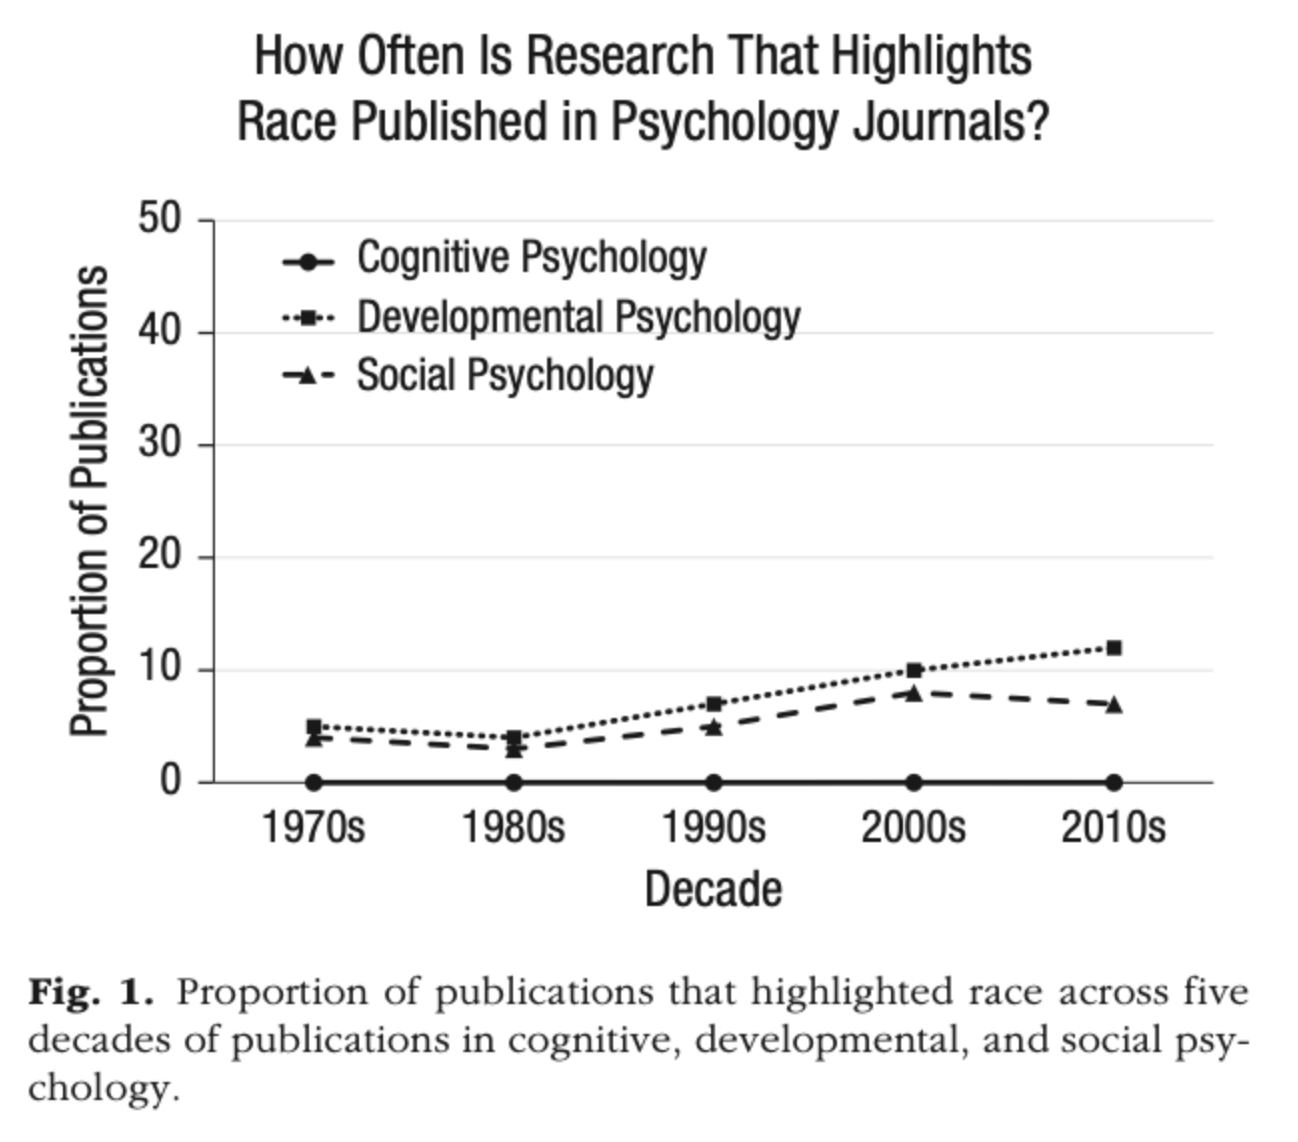
\includegraphics[width=4.94792in,height=\textheight,keepaspectratio]{images/1_RaceResearch.png}
\end{center}

As we'll discuss throughout this class, life is complex and there is
never one explanation for any phenomenon. However, it's important to
note that psychology as a field has historically been dominated by white
authors (researchers who write scientific papers) and white editors
(researchers who decide what papers get published or not).

\begin{center}
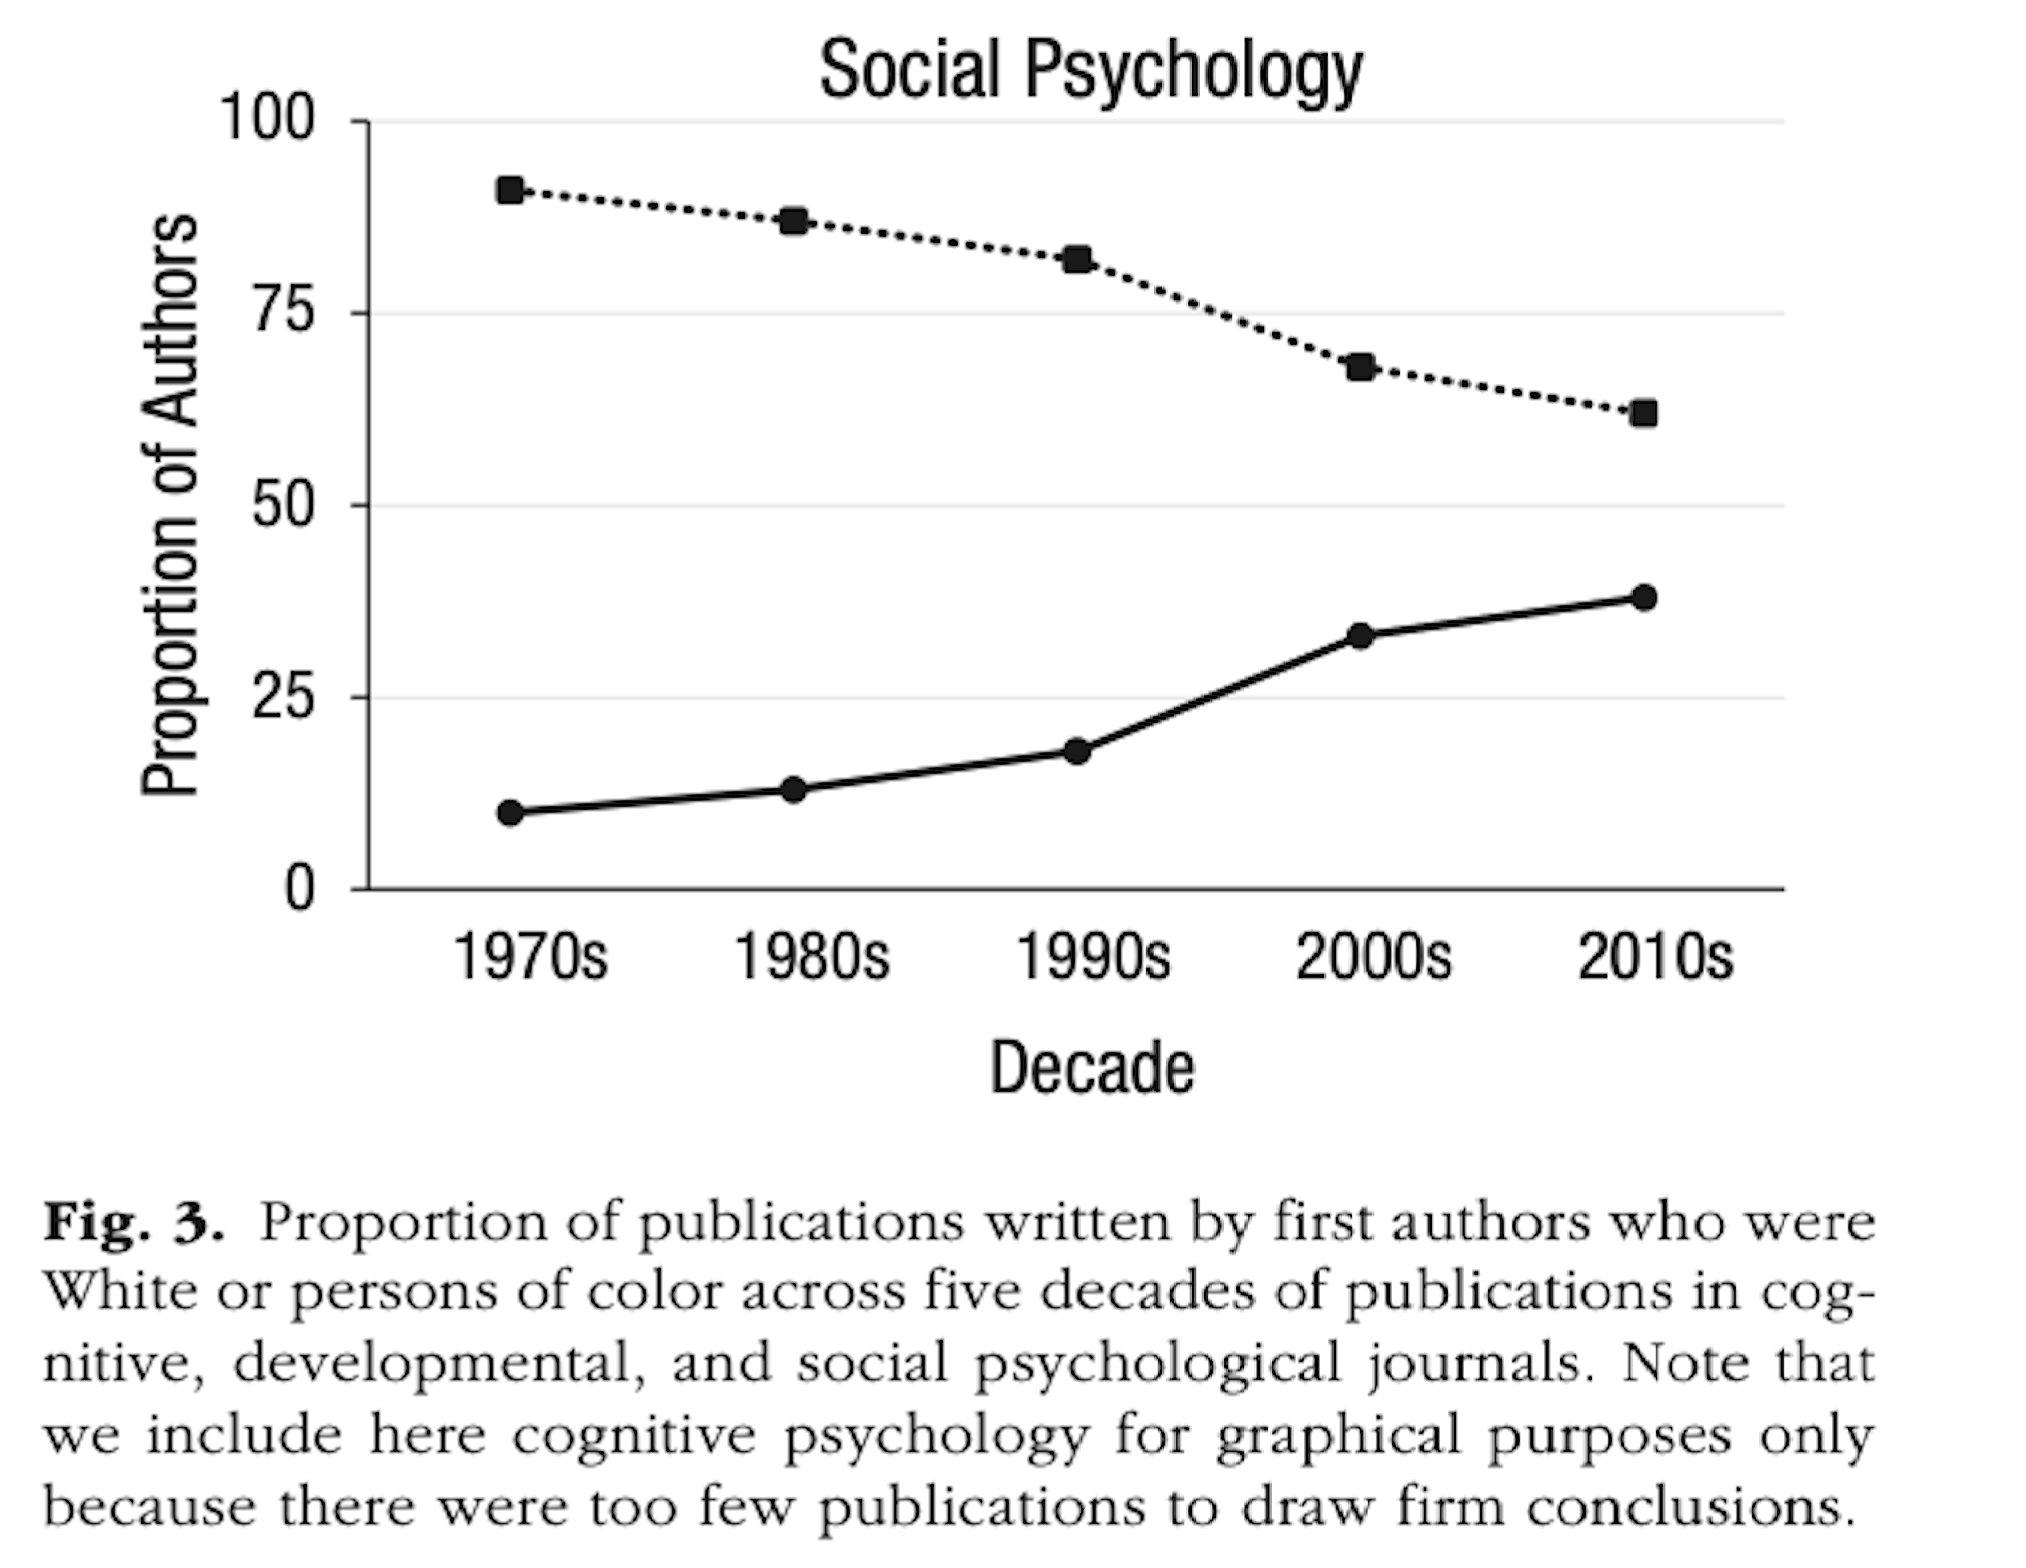
\includegraphics[width=4.94792in,height=\textheight,keepaspectratio]{images/1_white_authors.png}
\end{center}

These trends are important to reflect on, because they reveal a bias in
who becomes a psychologist, and what types of questions these
researchers are interested in pursuing.

It's also a goal of this class to not only highlight the important
contributions of non-white researchers and statisticians, but also make
sure that all students in this diverse classroom feels empowered to use
statistics, research methods, and R skills to ask (and answer) research
questions that matter to them!\footnote{This is the purpose of your
  final project! We'll talk more about this throughout the class.}

\subsection{Psychology as a REAL SCIENCE
™}\label{psychology-as-a-real-science}

Psychology uses statistics because, in part, it wants to establish
itself as a real science, like physics and chemistry. You don't have to
take my word for it, just look at the definitions of some common sources
of psychological knowledge - introductory textbooks:

\begin{itemize}
\item
  ``Today, we define psychology as the science of behavior and mental
  processes.'' (Myers, 2011)
\item
  ``\ldots the science of behavior and the mind.'' (Grey, 2010)
\item
  ``\ldots the scientific study of mind, brain, and behavior.''
  (Gazzaniga, 2010)
\item
  ``\ldots We now define psychology as the science of behavior and
  mental processes.'' (Myers \& DeWall, 2018)
\end{itemize}

I'm probably showing my age looking to textbooks, so let's check in with
ChatGPT\footnote{See the syllabus for the course ChatGPT policy. You may
  also be interested to read on the ethical and
  \href{https://bsj.studentorg.berkeley.edu/the-new-dimension-to-the-climate-crisis-chat-gpt/}{environmental
  issues} surrounding this emerging technology.} to see whether the
algorithmic summary of large piles of data suggests that psychology is,
in fact, a ``real science'' :~

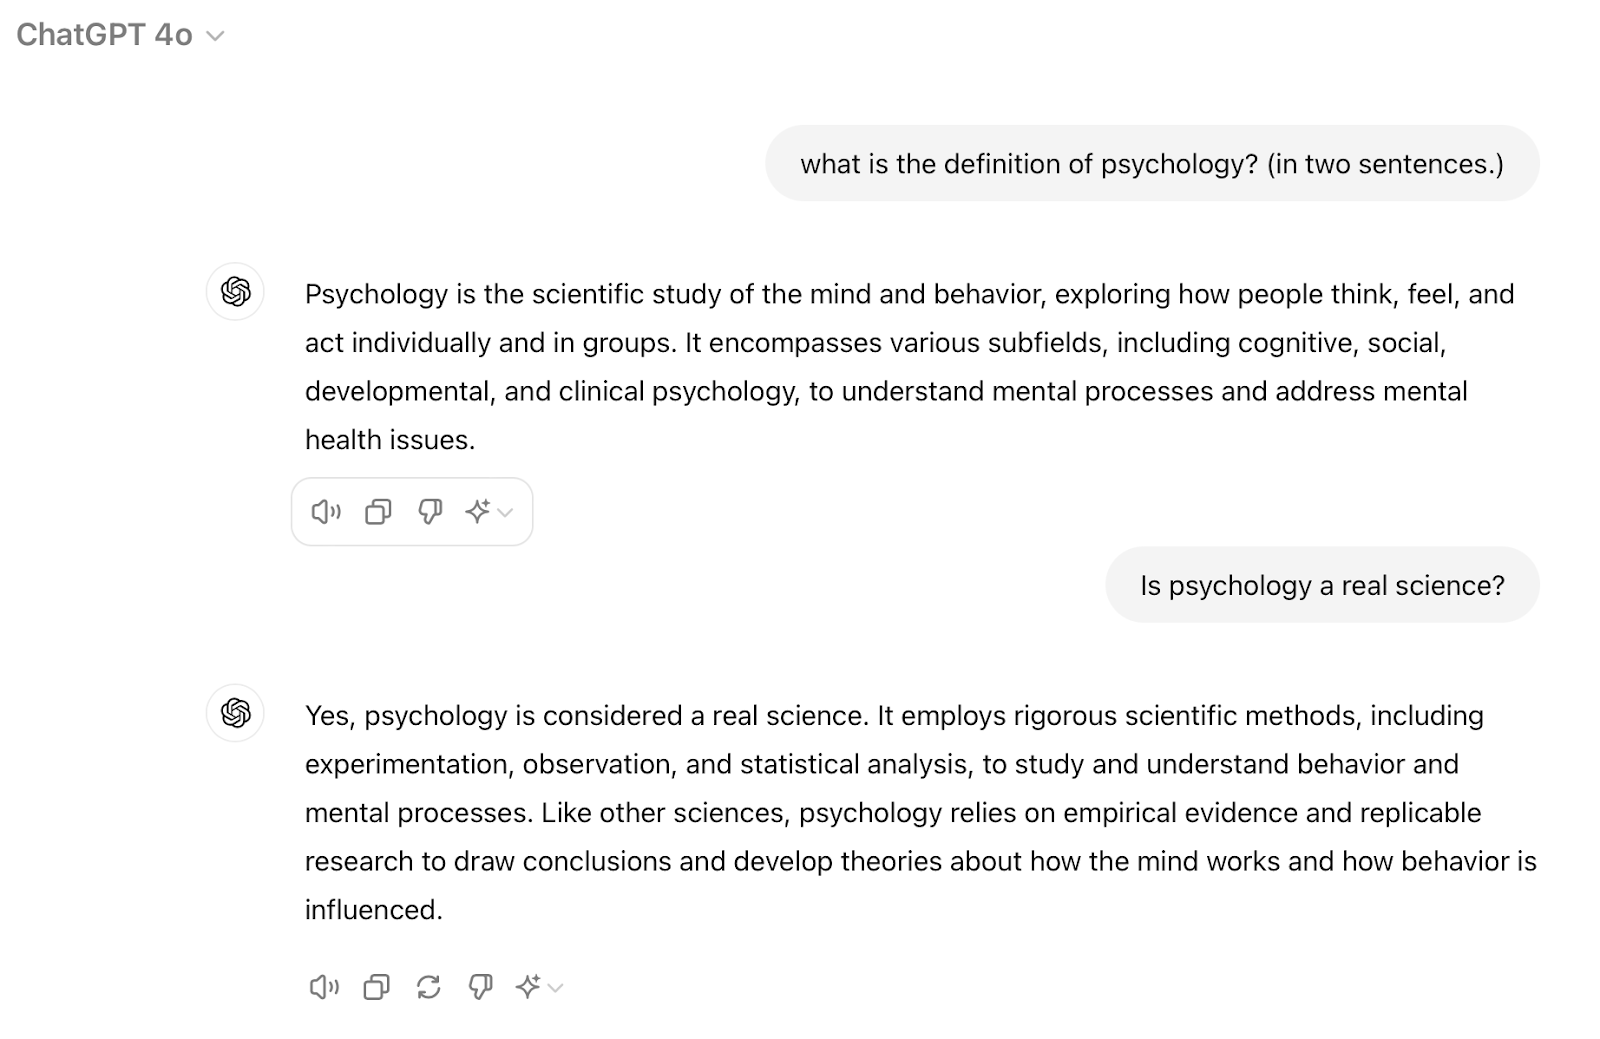
\includegraphics[width=4.94792in,height=\textheight,keepaspectratio]{images/1_psychsci_chatGPT_def.png}

Perhaps more authoritatively, the American Psychological Association
(APA) confirms that psychology is, ``the study of the mind and
behavior\ldots a diverse scientific discipline comprising several major
branches of research.'' (APA, 2024).

The consistent emphasis on science (and ``rigorous'' methods!) in these
definitions is an attempt to elevate psychology through language to the
status of other ``hard'' sciences, like physics and chemistry. But
inclusion of the term ``science'' also seeks to differentiate psychology
from its less scientific heritage and past, defend itself from
accusations from other scientists / talking heads (if not some of your
friends in STEM majors\ldots or parents) that it is not actually REAL
SCIENCE ™.~

\subsubsection{What is Science? Prediction (and
Error)}\label{what-is-science-prediction-and-error}

One of the most important goals of science is to form
\textbf{predictions}, and then use these predictions in order to
influence outcomes (a form of \textbf{power}).

A \textbf{prediction} is an educated guess you have about the future.
Educated means that the guess comes from some knowledge (either your
experiences, beliefs, something you learned in a textbook, or the
results of a scientific study). A prediction can have two outcomes :

\begin{itemize}
\item
  \textbf{Valid :} your prediction is right
\item
  \textbf{Error :} your prediction is wrong.
\end{itemize}

Of course, things are rarely as simple as ``right'' or ``wrong'', and a
large part of this class will be learning how to quantify exactly how
much error there is in our scientific predictions.

As an example, let's look to the stars.

\begin{longtable}[]{@{}
  >{\raggedright\arraybackslash}p{(\linewidth - 2\tabcolsep) * \real{0.1773}}
  >{\raggedright\arraybackslash}p{(\linewidth - 2\tabcolsep) * \real{0.8227}}@{}}
\toprule\noalign{}
\endhead
\bottomrule\noalign{}
\endlastfoot
\pandocbounded{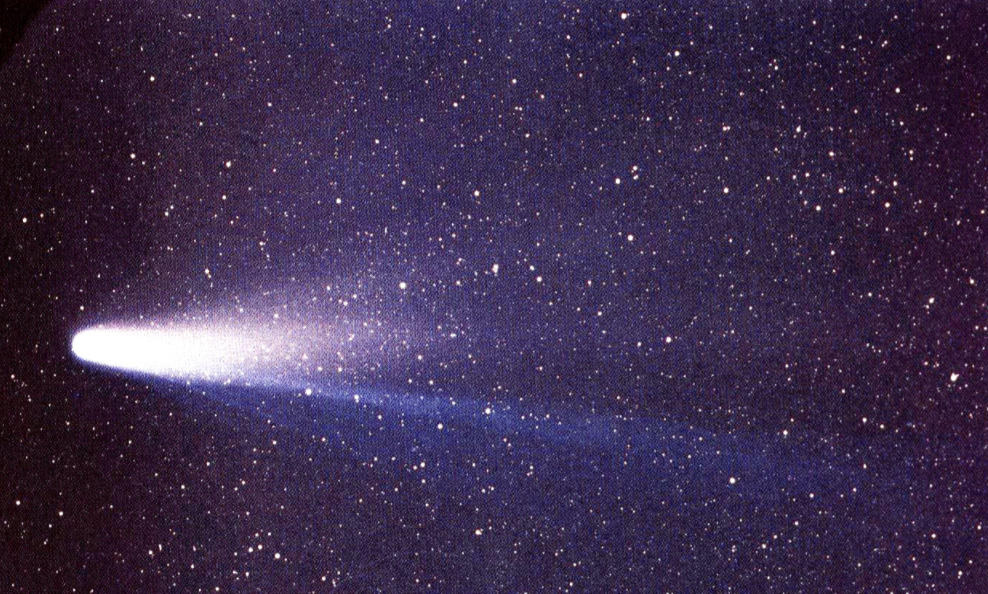
\includegraphics[keepaspectratio]{chapters/images/clipboard-3451448147.png}}
& Astronomers have developed knowledge about celestial bodies - gravity,
orbits, mass (I know very little about this).

But I trust this science because astronomers are able to use it to make
very valid predictions about giant space rocks and when they will come
close to the earth.\footnote{You can see when scientists predict
  Halley's comet to come closest to earth
  \href{https://theskylive.com/halley-tracker}{here}. While this is
  fairly accurate, I've seen the exact prediction change over the years
  - there is still some error in this prediction.}

I can use this knowledge to plan a stargazing trip, or plan to watch all
the rich people leave earth when the ``big one'' comes for the rest of
us. \\
\end{longtable}

As another example, on the day I'm writing these words, I do not predict
that it will rain outside. I am making this prediction based on the
following information :

\begin{itemize}
\item
  it did not rain yesterday
\item
  it is not currently raining
\item
  I live in Oakland, where it rarely rains in August.
\item
  the air doesn't have that feeling of rain; that smell.
\item
  I looked at the weather forecast app and it said we had a week of
  sunny weather ahead.
\item
  \href{https://walzr.com/weather-watching}{Nobody was carrying an
  umbrella today}.
\item
  there are no clouds.
\end{itemize}

Because I predict it will not rain, I'm not too worried that the tarp is
not covering my bike locked outside. Of course, my prediction could be
wrong.

\marginnote{\begin{footnotesize}

\begin{center}
\pandocbounded{
\includegraphics[keepaspectratio]{chapters/images/1_puffinrain.png}}
\end{center}
It sometimes rains when sunny, as on Puffin Rock, where we'll be here
come rain or shine.

\end{footnotesize}}

For our first lecture, start thinking of some predictions that you have
made. What knowledge informed the prediction? Did you use this
prediction to influence your future behavior in some way? What kinds of
predictions do psychologists make? We will chat more about these ideas
in class :) but it's a core focus on why psychologists use predictions.

And so, here we are. In this document, in this required class for the
psychology major, learning how to DO REAL SCIENCE. With statistics.

\subsubsection{Linear Models to Organize Our
Predictions}\label{linear-models-to-organize-our-predictions}

The linear model a simple formula that helps researchers to make, and
quantify, their predictions. We will talk much more about linear models
in our class - they are one of the most important concepts we will cover
and a foundation of modern statistics - but for now let's just focus on
the basics :

A linear model takes the following form: \footnote{I can already feel
  some of y'alls math anxiety rising across time and space. But
  remember, stats is just a language with some vocabulary we need to
  learn.}

\[
DV \sim IV_1 + IV_2 + ... + IV_k + \epsilon
\]

Below is a description of terms in the model :

\begin{itemize}
\item
  \textbf{DV = dependent variable.} This is the variable that you want
  to predict. It's up to the researcher what variable is the dependent
  variable. More complicated models can have more than one DV, but for
  this class we will just focus on one DV at a time.
\item
  \textbf{IV = independent variable.} This is a different variable that
  you think will help you make predictions. Again, it's up to the
  researcher to choose what variables they will include to try and make
  predictions of the DV.
\item
  \textbf{k = any number.} This is a way of saying that there can be
  many IVs. Life is complex, and so in order to predict one variable, we
  will need to use information from lots of other variables.
\item
  \textbf{\textasciitilde{} = a squiggly line / tilde.} I like to use
  the squiggly line to reinforce the idea that our model is uncertain
  and squiggly (this is not an exact prediction where an equal sign
  would be used). R also uses the tilde for defining a model, so it's
  nice to start practicing stretching our pinkie finger to reach that
  upper left corner of the keyboard.
\item
  \(\epsilon\) \textbf{= error =} this term always concludes our written
  model, and accounts for the many other reasons why our predictions
  might be wrong. This could be because we haven't included certain
  variables that are important to make predictions (either because we
  can't measure them in our study, don't think they are important enough
  to study, or don't know that we should study them), or because we are
  measuring our variables with some amount of error\footnote{We will
    learn more about \emph{measurement error} in Chapter 4.}.
\end{itemize}

For example, I could write out my prediction about rain as the following
linear model :

\begin{itemize}
\tightlist
\item
  rain \textasciitilde{} clouds + umbrellas + weather app status + smell
  + air pressure + season + location + temperature + error
\end{itemize}

We read a model as : ``the DV is a function of\ldots{}'' or sometimes
``the DV depends on\ldots{}''. So I'd read this model as ``rain is a
function of clouds, umbrellas, the weather app status\ldots etc.'' And
it's good practice to leave the variables neutral (e.g., just
``clouds'', not ``storm clouds'').\footnote{Later we will talk about
  ways to account for the fact that more umbrellas increases the chance
  it will rain in our model.}

Error in this model would represent the fact that I haven't accounted
for some important variables that we know we should include (like
humidity, coastal pressure systems, or palnetary waves), the fact that
some of my variables were probably measured with error (was no one
\emph{really} carrying an umbrella???), and the fact that there are some
things that we don't know about rain, and what predicts it (this is what
weather scientists are trying to learn more about.)

Once we add numbers and data to a linear model\footnote{We will get to
  this in Chapter 6!}, we can quickly see :

\begin{itemize}
\item
  which variables allow us to make the best predictions, and which
  variables do not improve our predictions (e.g., is the number of
  umbrellas others are carrying a good predictor of whether it's going
  to rain or not?)
\item
  the direction of the relationship between each IV and the DV (e.g., is
  it that more umbrellas = more rain, or more umbrellas = less rain?)
\item
  the amount of error in our predictions (e.g., how good, exactly, is
  this model at predicting the rain?)
\end{itemize}

\paragraph{Practice Writing A Model}\label{practice-writing-a-model}

Imagine a researcher wants to better understand why people differ in
happiness, and believes that playing music, drinking more water, and
eating ice cream sandwiches are important factors to consider. How would
you write this out as a linear model?

\begin{tcolorbox}[enhanced jigsaw, toptitle=1mm, toprule=.15mm, rightrule=.15mm, breakable, left=2mm, colbacktitle=quarto-callout-caution-color!10!white, colback=white, opacityback=0, coltitle=black, bottomtitle=1mm, opacitybacktitle=0.6, titlerule=0mm, leftrule=.75mm, arc=.35mm, bottomrule=.15mm, title=\textcolor{quarto-callout-caution-color}{\faFire}\hspace{0.5em}{Click Here to See The Answer}, colframe=quarto-callout-caution-color-frame]

happiness \textasciitilde{} music playing + water intake + ice cream
consumption + error

For this model, I've organized the focus of the research question on the
left-hand side and listed the three other variables to the right, using
neutral descriptions (e.g., `water intake' rather than `drinking more
water'). I also included error at the end of my model to account for the
fact that some people who play music, drink water, and eat ice cream
are, in fact, not happy. I also didn't add other varibles that might be
related to happiness, since these were not part of the researcher's
statement.

\end{tcolorbox}

\section{Part 2 : Why R?}\label{part-2-why-r}

This semester, we will also learn how to use the computer programming
language R to work with data, conduct analyses, and make graphs. R can
be intimidating to work with at first, and is more confusing than it
needs to be sometimes (as you'll quickly find out\ldots), but I promise
you will learn!\footnote{In fact, that's the point of this class.} It's
totally okay (and expected) for you to feel frustrated at times; this is
part of the learning process. So please embrace the ``I HAVE NO IDEA
WHAT I'M DOING'' dog meme energy (and look how happy the doggy looks!)
as you embark on your R journey.\\

\begin{longtable}[]{@{}ll@{}}
\toprule\noalign{}
\endhead
\bottomrule\noalign{}
\endlastfoot

\includegraphics[width=2.86458in,height=\textheight,keepaspectratio]{chapters/images/R_logo.svg.png}
&
\pandocbounded{
\includegraphics[keepaspectratio]{chapters/images/r_meme_dog.png}} \\
\end{longtable}

\subsection{Installing R}\label{installing-r}

\href{https://posit.co/download/rstudio-desktop/}{\textbf{Use this link
to Download and Install the Programs R and RStudio Desktop}}

{\textbf{Note : You must download both R and RStudio Desktop (these are
two separate programs). Make sure to download the most recent version of
R and RStudio to avoid issues in the future.}}

\begin{enumerate}
\def\labelenumi{\arabic{enumi}.}
\item
  \textbf{R} is the powerful, free, and somewhat intimidating computer
  program that we will use to analyze data in this class. This website
  is not super friendly - choose the operating system you have (Windows,
  MacOS, or Linux) and then download the ``latest release'' on the next
  page. \textbf{If you have a chromebook or iPad / tablet, you will need
  to use \href{https://rstudio.cloud/}{posit.cloud}.}
\item
  \textbf{RStudio} is an Integrated Development Environment (IDE) -
  basically a ``home'' for R to live in, with rooms and this program is
  not 100\% necessary, but makes it a little easier to navigate R. Note
  that you will need to install R first in order for RStudio to work.
\end{enumerate}

\textbf{Having trouble getting these programs to work?}

\begin{enumerate}
\def\labelenumi{\arabic{enumi}.}
\item
  \textbf{Here's \href{https://www.youtube.com/watch?v=0Qu7Jg1Jw5A}{one
  YouTube video}} someone made to show you how to download and install.
\item
  \textbf{Try \href{https://posit.cloud}{posit.cloud}}. This is a
  web-based version of RStudio, and has a free option but limits your
  hours of work each month. There's a paid option for \$5/month that you
  can use if you sign up with your student e-mail address; former
  students also pointed out that you can always create a new ``free''
  account if you run over the 15-hour limit.
\item
  \textbf{Ask for help!} The professor, other students, or a tutor /
  your TA can help get everything working properly.
\end{enumerate}

\subsection{Navigating R}\label{navigating-r}

Watch the two videos below for a quick introduction to R - the program
we will be using to analyze data.

\subsubsection{VIDEO : Navigating R}\label{video-navigating-r}

\url{https://youtu.be/TDt8x4ASZoc}

\begin{itemize}
\item
  what R looks like when you open it
\item
  basic math in the~\textbf{console}
\item
  indexing and output
\end{itemize}

\subsubsection{VIDEO : Navigating
RStudio}\label{video-navigating-rstudio}

\url{https://youtu.be/on5oPls94oU}

\begin{itemize}
\item
  what RStudio/Posit looks like; navigating the program
\item
  basic math in the console
\item
  the~\textbf{source file}~(makes life easier and saves your work!)
\end{itemize}

\section{Part 3 : How Science? The Scientific Method in Five Easy
Steps}\label{part-3-how-science-the-scientific-method-in-five-easy-steps}

The Scientific Method is used to help science progress toward valid
(accurate, ``true'') predictions and avoid biases. This is the same
scientific method you may have learned about in a previous science class
or used for a science fair project\footnote{~~Do elementary school
  students still do those science fair projects with the tri-fold
  posters? Adult scientists do the same kinds of science fairs, except
  they are called ``conferences'', involve a little more math, and use
  flat posters. I also don't think anyone gets ribbons (status among
  scientists takes other less concrete forms). Some of the largest
  conferences include that held by the
  \href{https://convention.apa.org/}{American Psychological Association}
  or the
  \href{https://www.psychologicalscience.org/conventions}{Association of
  Psychological Science}. The
  \href{https://westernpsych.org/convention/}{Western Psychological
  Association} has a more local conference, and there are literally
  hundreds of other conferences based on research topic (for example,
  the \href{http://meeting.spsp.org/}{Society of Personality and Social
  Psychology}). If you are interested in learning more about
  conferences, ask your GSI what conferences they attend. And you even
  might be able to present your project in this class as a conference
  poster - no tri-fold needed.}.

I like to organize the scientific method into five broad parts,
described below.

\subsection{Step 1 : Identify a
Question}\label{step-1-identify-a-question}

First, a researcher starts with a question about the variable that they
want to predict or the psychological phenomenon they are interested in.
In Part 1 of this chapter, we talked about how these questions are often
informed by the researcher's own observations or experiences. In this
section, we'll discuss ways you can choose a topic to inspire a specific
research question - something you will do as part of your final project
in this class.

We'll talk about this more in class, but the basic idea is that you will
identify a topic that you care about, develop this idea into a research
question, design a study to answer some part of this question, collect
and analyze the data from your study (using R!), and then write up the
results as an academic paper.

The first step, is picking some topic or variable that you care about,
and identifying the parts of your background or experiences that
influence this topic. This can be a challenging first step, and it's
okay to struggle. Your topic will also change as we develop it, so don't
feel like it needs to be ``perfect'' or ``locked in'' yet.

Looking for project topic inspiration? A few ideas to consider :

\begin{itemize}
\item
  \textbf{Think about why you become a psychology major.} Was it because
  you were interested in people, find dreams fascinating, wonder if you
  could get good at detecting people's lies? Think about these
  interests, then think about what variables might be relevant. For
  example, while you won't have access to an fMRI machine (or the
  required statistics) in order to
  \href{https://www.youtube.com/watch?v=inaH_i_TjV4}{reconstruct images
  people see during their dreams}, you might study people's beliefs
  about the importance of their dreams, or the extent to which they have
  dreams.
\item
  \textbf{Focus on a problem you've encountered or observed in
  real-life.} Notice that something in the world could be better? How
  would you label that as a variable? For example, maybe you want to
  better understand people's attitudes about capitalism or racism or
  housing costs.
\item
  \textbf{Look at faculty webpages, and see what they (and / or their
  graduate students) are studying.} Does anything seem interesting to
  you? Who looks like they might be cool to work with? What aspects of
  their research question might you study with this project?
\item
  \textbf{Chase the latest trends of today.} Identify the new hot trend
  in our capitalist society these days, and then focus your project on
  that. For example, you could examine how people's perceptions of
  HOTNEWTREND are influenced by some aspect of their identity, or how
  exposure to HOTNEWTREND influences people's affect, behavior, or
  cognition (compared to another HOTTREND, or maybe an OLDTREND).
\item
  \textbf{You don't have to take my word for it.}
  \href{https://libguides.usc.edu/writingguide/introduction/researchproblem}{Here's
  another guide} that might offer some help, or ask for help in the
  class discord / office hours / lecture!
\end{itemize}

Once you've chosen your topic, make sure that it's the right level of
focus, and something you can complete with the resources you have.

\begin{longtable}[]{@{}
  >{\raggedright\arraybackslash}p{(\linewidth - 6\tabcolsep) * \real{0.1156}}
  >{\raggedright\arraybackslash}p{(\linewidth - 6\tabcolsep) * \real{0.4532}}
  >{\raggedright\arraybackslash}p{(\linewidth - 6\tabcolsep) * \real{0.2789}}
  >{\raggedright\arraybackslash}p{(\linewidth - 6\tabcolsep) * \real{0.1486}}@{}}
\toprule\noalign{}
\begin{minipage}[b]{\linewidth}\raggedright
Initial Topic
\end{minipage} & \begin{minipage}[b]{\linewidth}\raggedright
Problem
\end{minipage} & \begin{minipage}[b]{\linewidth}\raggedright
Ways to Revise Without Sacrificing Your Vision
\end{minipage} & \begin{minipage}[b]{\linewidth}\raggedright
Example Revised Version
\end{minipage} \\
\midrule\noalign{}
\endhead
\bottomrule\noalign{}
\endlastfoot
Why do people do the things that they do?

How does social media influence mental health? & Great start, but these
topics are too broad! Which things? Which people? What aspects of mental
health? & Try to focus by identifying a specific aspect of people's
affect, behavior, or cognition that you care about, or a specific group
of people to study. & Why do people overshare personal details in social
settings?

How does social media usage influence social anxiety in teenagers? \\
Do sociopaths dream about kittens more than non-sociopaths?

How does inter-generational trauma change our neural wiring? &
Interesting topics! However, it would be really difficult to study with
the resources that a student in this class would have. (e.g., it would
be hard to find sociopaths to give surveys to; hard to rent out an fMRI
to measure voxel activation.) & Think about ways to adapt the question
to account for people that you could study, and variables that you could
more easily measure. & How do dreams influence people's future behavior?

What are some strategies that help people heal from inter-generational
trauma? \\
\end{longtable}

\begin{tcolorbox}[enhanced jigsaw, toptitle=1mm, toprule=.15mm, rightrule=.15mm, breakable, left=2mm, colbacktitle=quarto-callout-tip-color!10!white, colback=white, opacityback=0, coltitle=black, bottomtitle=1mm, opacitybacktitle=0.6, titlerule=0mm, leftrule=.75mm, arc=.35mm, bottomrule=.15mm, title=\textcolor{quarto-callout-tip-color}{\faLightbulb}\hspace{0.5em}{Prof.~Cat Has An Idea}, colframe=quarto-callout-tip-color-frame]

Hi folks, Prof.~Cat here. I'll be popping up throughout this book to
guide you through the process of working on your final project. To do
this, I'll work on an example along the way.

\textbf{Choosing a Topic and Reflecting on the Ways Your Background
Influences (and maybe biases) You :} I'm interested in the (negative)
consequences of looking at images of war-torn cities on people's
attitudes about the inhabitants. Specifically, I'm wondering if seeing
these images of destroyed cities - and the screaming or injured citizens
who live in them - leads people to (unintentionally) dehumanize these
people by seeing them only as powerless victims, and not inhabitants
with culture, family structures, etc. This interest is inspired by a few
different things - I've seen a lot of horrifying images from Gaza in the
last few years, but less emphasis or coverage about how these people are
(and were) living before being bombed. I also have always been really
critical of war and the US war machine as a kid (due to the influence of
my parents, some books, Miyazaki films, a few teachers, and a minister).
I'm also half-Iranian, so am biased to pay more attention to this part
of the world (and the long history of conflict with the US), and
probably am biased to see victims from this region in more humanizing
ways because of the many cultural similarities (in language, music,
dress, religion, love of tea, etc.)

\end{tcolorbox}

\marginnote{\begin{footnotesize}

\begin{figure}[H]

{\centering 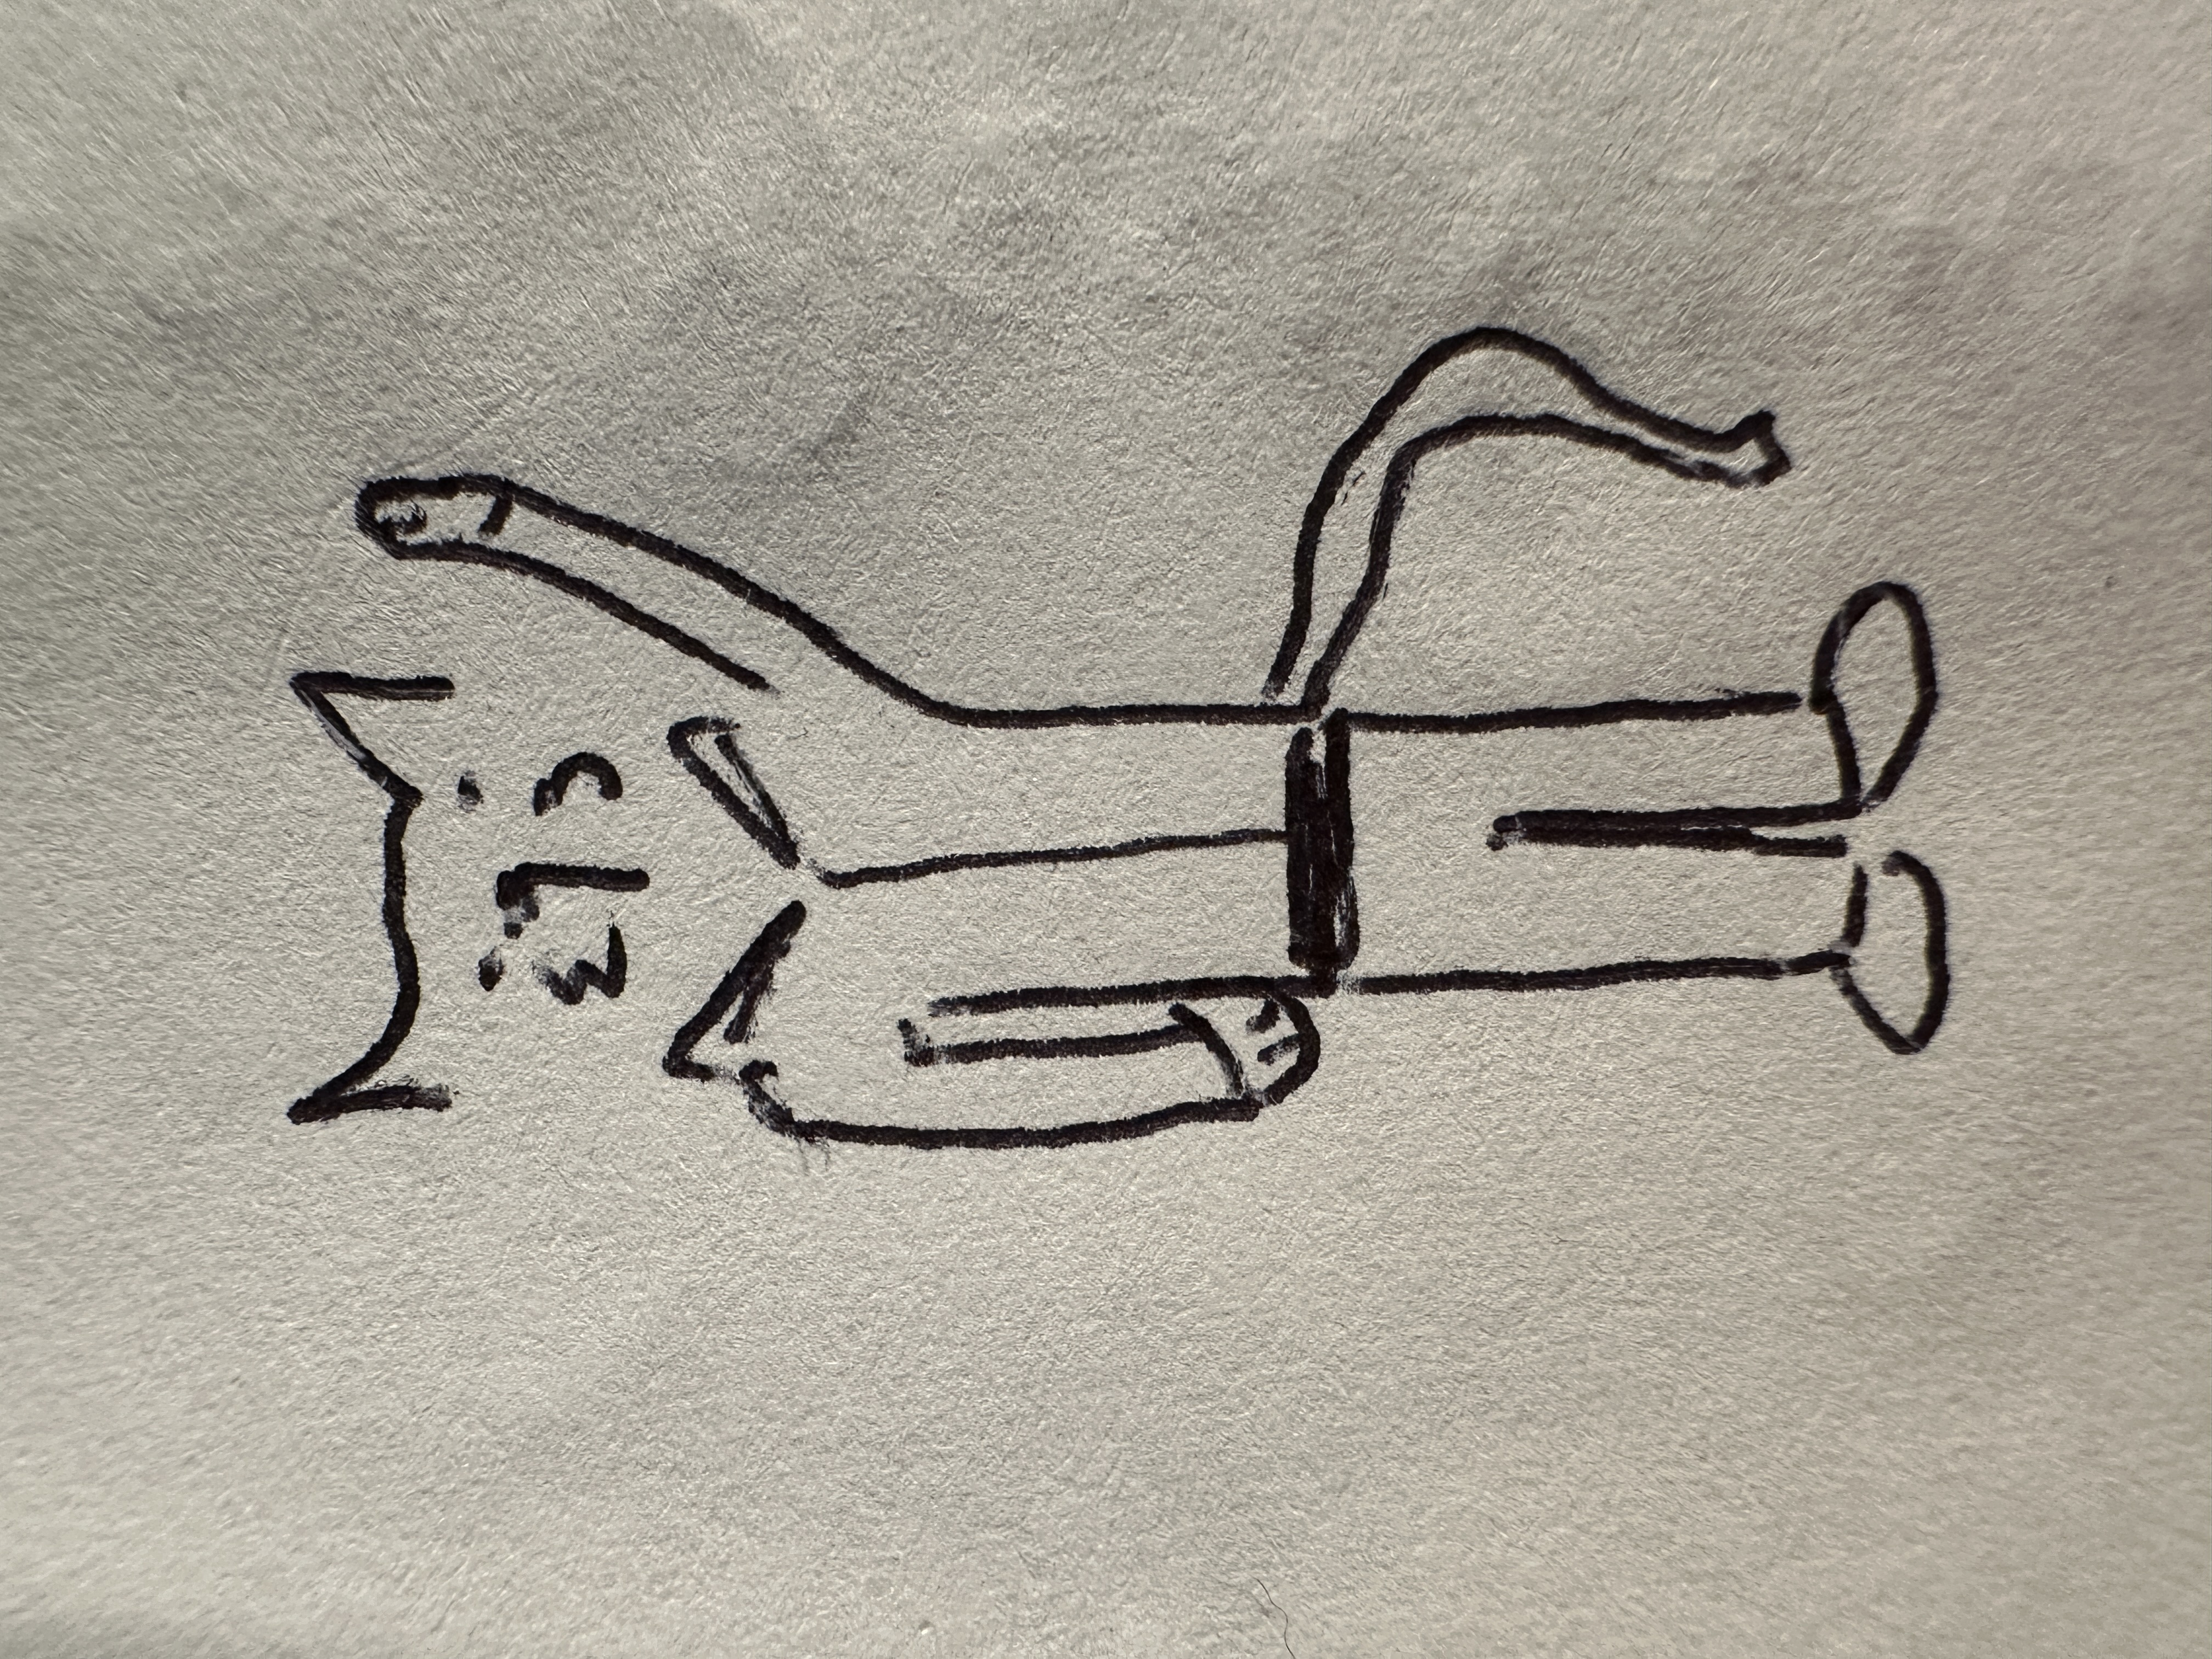
\includegraphics[width=1.41667in,height=\textheight,keepaspectratio]{chapters/images/1_profcathi.JPG}

}

\caption{hi, says prof. cat}

\end{figure}%

\end{footnotesize}}

\subsection{Step 2 : Develop a Theory}\label{step-2-develop-a-theory}

A scientific theory is one that is comprehensive, explanatory, and
supported by evidence. For example, the theory of evolution is
\emph{comprehensive} (it relates to all nature, not just plants or
animals or finches), it is \emph{explanatory} (it's why we and
\href{https://www.gutenberg.org/files/1227/1227-h/images/fig15.jpg}{cats}
both narrow our eyes when we are scared and angry), and it is
\emph{supported} (by over 100 years of evidence\footnote{\href{https://evolution.berkeley.edu/evolibrary/article/0_0_0/lines_01}{From
  fossil records to observations of fruit flies and plans}}).~

\textbf{Most scientists refrain from saying that a theory is ``proven''
or ``true'' for two reasons:}

\begin{enumerate}
\def\labelenumi{\arabic{enumi}.}
\item
  First, the scientific method is a process - our knowledge and ideas
  are continually updated. So it's likely that the theory of evolution
  will be updated as we learn more about the complex ways genes
  replicate and interact with the environment. Saying that a theory is
  ``proven'' is a common mistake - watch out for it!~
\item
  Second, most scientists (and psychologists) draw from Karl Popper's
  philosophy of science, which adheres to a requirement for science
  called \textbf{falsifiability -} the ability to find evidence that
  rejects a theory (``ability to falsify''). This means a theory is
  never `proven' because scientists are continually looking for evidence
  to reject the theory. It also means that a belief that cannot be
  tested or rejected would be rejected as a scientific belief - you have
  to be able to test your belief in some observable way. Falsifiability
  is where I think science separates from religious belief - someone
  with faith doesn't need evidence, and that's okay! It just doesn't
  make the belief scientific under science's narrow definition.~
\end{enumerate}

\textbf{Hypotheses} are specific predictions that researchers make about
what they expect to see in the data if their theory is supported or is
not supported by data.~

\begin{itemize}
\item
  The \textbf{alternative hypothesis} (sometimes written \textbf{HA}) is
  the researcher's own belief. It may seem strange to label your belief
  ``alternative'' when this word is used for things that are supposed to
  be different (``alternative rock = it's not your parent's rock \&
  roll!''), and we are so used to thinking that our beliefs are the
  default that to call them alternative seems wrong. This is an example
  of previous beliefs bias, and the decision to label our beliefs as the
  ``alternative'' is an example of science trying to correct this bias.
  It's a small and symbolic correction, but it's better than nothing.
\item
  The \textbf{null hypothesis} (sometimes written \textbf{H0}) is the
  label given for whatever evidence would not support the researcher's
  belief.
\end{itemize}

\textbf{EXAMPLE :} Let's say you believe that smoking cannabis hurts a
person's memory. What's the alternative hypothesis? What's the null?

\begin{itemize}
\item
  \textbf{Null Hypothesis :} People who smoke cannabis will perform
  BETTER or NO DIFFERENT on a memory test than people who do not smoke
  marijauna. \footnote{Many students forget to include the ``NO
    DIFFERENT'' in the null hypothesis example above. However remember
    that the null hypothesis is everything that your theory is not. So
    if your theory is that smoking cannabis HURTS memory, then finding
    no difference in the memory of pot smokers vs.~non-smokers would not
    support your theory, and is thus part of the null hypothesis. (Note
    : some of y'all may have missed this because you are remembering
    learning about ``directional'' vs ``non-directional'' hypotheses -
    we will discuss this more in Lecture 8.)}
\item
  \textbf{Alternative Hypothesis :} People who smoke cannabis will
  perform WORSE on a memory test than people who do not smoke marijauna.
\end{itemize}

\href{https://docs.google.com/forms/d/e/1FAIpQLSdPgseWI3odCwC34jvRZGe0H4oz0Et4HwG8xTig5YFtDU_ldw/viewform?usp=header}{\textbf{Practice
: Identifying Models, Null, and Alternative Hypotheses}}\textbf{.}
Here's a quick practice quiz to review identifying models based on
research questions and theories, and identifying the null and
alternative hypotheses based on a given theory.

\subsection{Step 3 : Collect Data}\label{step-3-collect-data}

As described above, scientific theories are supported by evidence called
data. How researchers collect data is something we will discuss in more
detail over the next few weeks. In general, researchers have to figure
out how to measure the variables they are interested in studying (e.g.,
``how will I know if someone is happy or not?''), and then find
participants (people or animals) to study (e.g., ``whose happiness
should I study'').~

For example, in our smoking cannabis example the decisions about how to
measure memory (a music memory game or a word recognition task?) or how
much cannabis (a little or a lot?) or who to study (Berkeley students or
your grandparents?) in the study would likely influence the results.

The decisions that researchers make about how to define their measures
and the participants they will study are very important, and will
influence the results of the study (and thus our knowledge of the
topic), so stay tuned for more discussion!

\subsection{Step 4 : Use Data to Test
Theories}\label{step-4-use-data-to-test-theories}

Finally, researchers look to see if the data they collected supports or
rejects their theory (and evaluate how strongly their theory is
supported or rejected). We'll talk much more about using data to test
theories this semester.

In our smoking cannabis example, the researcher would look to see which
group did better on the memory test, and if the smokers did worse, then
their theory would be supported (by this one study, at least).

\subsection{Step 5 : Repeat}\label{step-5-repeat}

Once a study is completed, researchers repeat the scientific method in
two different ways.

Researchers will sometimes repeat the exact same steps a second time -
something called \textbf{replication}. Replication is critical to
science.

Scientists also repeat the scientific method with a new question that is
based on the results from their first study. Science is a process, and
researchers are never done learning about how to better predict \&
control the world. There's always more research to do. For example,
after identifying a pattern between smoking cannabis and memory, a
researcher might ask whether the type or dosage of cannabis intake would
influence memory, whether abstinence could reverse the effects of memory
impairment, or whether cannabis and coffee together might lead to a
different result. Note that this is not an example of replication, since
researchers are not testing the same question they had - but it's
repeating the scientific method for a new question inspired by the old.
This is good, and part of scientific progress. But the problem is that
the incentives for scientific publication focused almost entirely on
``new'' research, and not really making sure that the ``old'' research
was valid.

\subsection{It's Never Actually Easy}\label{its-never-actually-easy}

Science is hard, and people are very complex, which makes psychological
science very hard. Unfortunately, psychology is in a bit of a
\href{https://www.vox.com/future-perfect/21504366/science-replication-crisis-peer-review-statistics}{Replication
Crisis}. This crisis is two-fold a) researchers tend not to seek to
replicate their (or others') results, and b) systematic attempts to do
so have suggested that the majority of results in psychology do not
replicate\footnote{You can go deeper into some of the drama surrounding
  the replication project \hyperref[0]{here}. lemme know what you think
  on the discord thread for this week.}.

We will chat more about this in our next lecture. But I think that's
enough reading for now?

\chapter{In Lecture.}\label{in-lecture.}

This week in lecture, we will get practice working in R (and define some
variables), talk more about the work that psychological researchers do,
and start learning how to develop your own interests into a final
project topic that you are excited to work on. Yeah!

\chapter{Data Data Data}\label{data-data-data}

Hello students! We are back. In this week's reading, you'll learn how to
work with data in R - first how psychologists define data, then how to
graph (and think critically about) different types of data with your
HUMAN BRAIN, and finally how to work with data (and datasets) in R.

\begin{figure}[H]

{\centering \pandocbounded{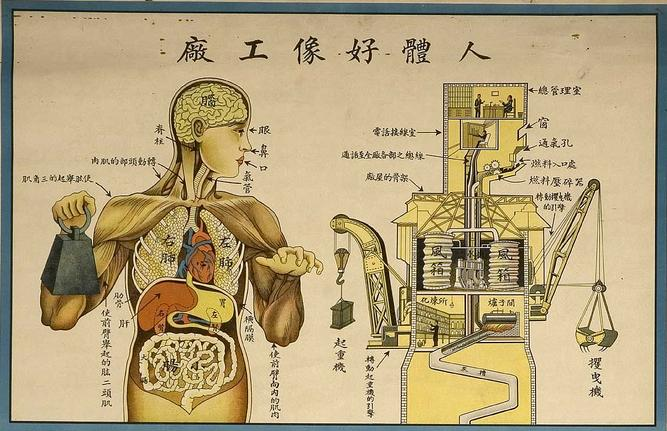
\includegraphics[keepaspectratio]{chapters/images/2_medicalposter.jpg}}

}

\caption{Chinese medical poster, 1933 (ref
\href{https://www.nlm.nih.gov/hmd/chineseposters/understanding.html}{US
NLM}; image source
\href{http://www.notechmagazine.com/2009/06/the-body-is-a-machine.html}{here})}

\end{figure}%

\begin{tcolorbox}[enhanced jigsaw, toptitle=1mm, toprule=.15mm, rightrule=.15mm, breakable, left=2mm, colbacktitle=quarto-callout-important-color!10!white, colback=white, opacityback=0, coltitle=black, bottomtitle=1mm, opacitybacktitle=0.6, titlerule=0mm, leftrule=.75mm, arc=.35mm, bottomrule=.15mm, title=\textcolor{quarto-callout-important-color}{\faExclamation}\hspace{0.5em}{To-Do List:}, colframe=quarto-callout-important-color-frame]

\begin{itemize}
\tightlist
\item
  Read this document and watch the videos to learn how to\ldots{}

  \begin{itemize}
  \tightlist
  \item
    define different types of data, and using your human brain to
    understand these data (Part 1).
  \item
    use R to define variables, import datasets, and navigate these
    datasets (Part 2).
  \item
    navigate the big business of academic research, and find research
    articles relevant to your interests (Part 3.)
  \end{itemize}
\item
  Take the practice exam (on navigating and loading datasets) in Part 2.
\item
  Take Quiz 2.
\end{itemize}

\end{tcolorbox}

\chapter{Part 1 : Defining Data}\label{part-1-defining-data}

Researchers seeking to bring a scientific approach to psychology love
data, and aim to convert complex human thoughts, feelings, and behaviors
into numbers. This is called \textbf{quantitative data,} and is the
default approach almost all modern research psychologists take. For
example:~

\begin{itemize}
\item
  Psychologists will quantify \textbf{affect} using heart rate monitors,
  finger temperature gauges, or even simple rating scales of how people
  are feeling (quick, how bored are you right now on a scale from 0 (not
  bored; super engaged professor!) to 10 (\ldots.most bored ever;
  surprised I'm even reading this right now)\ldots.see, you are just a
  number!)
\item
  Psychologists often quantify \textbf{behavior} by measuring reaction
  time, the number of times a person fidgets in a chair, how far a
  person will sit from another person in a study, the speed of a group.
  And even qualitative data - like a person's journal entry - would be
  turned into hard numbers by a researcher (who would ask a team of
  research assistants to read the journal and then count or provide a
  subjective rating to what they observe. this is called
  \textbf{behavioral coding}; we'll learn about it later. remind me if I
  forget.)
\item
  Neuroscientists quantify \textbf{cognition} in terms of voxel
  activation in the brain, or a sleep researcher might ask participants
  to write down their dreams in a journal, which then a team of research
  assistants would read and convert into\ldots.you guessed
  it\ldots numbers (e.g., number of times person dreamt about water or
  their parents; how stressful the dream seemed to the reader; etc.)
\end{itemize}

While we will learn more about the various ways psychologists collect
data later this semester, for now it's important to acknowledge that
these numbers have error (called \textbf{measurement error}), a fair
amount of work in psychology goes into learning how to reduce
measurement error as much as possible, and the existence of measurement
error is one form of error that will contributes to the ERROR term in
our linear models.

Quantitative data takes two forms that we will see in this class -
\textbf{numeric} (sometimes called \textbf{continuous data})~ and
\textbf{categorical data (}sometimes called ``string'' data).~

\section{Numeric Variables}\label{numeric-variables}

\subsection{Definition : Numeric
Variable}\label{definition-numeric-variable}

Numeric variables are when the value of the variable is a number (e.g.,
your Extraversion score is 62 on a scale from 0 to 100; or you said
``um'' fifty times yesterday, or scrolled your phone five times since
starting this reading.~

\textbf{Continuous variables} are a special type of numeric variable,
with the idea that values of the variable represent an ``infinite''
range of possibilities.

We often simplify complexity into discrete groups, but for most complex
phenomena, I believe that it's best to think of life as a spectrum. For
example, while I look at my walls and say ``they are blue'', a physicist
who really understands color theory would be able to interpret the
wavelength of light that is being reflected off these walls, and
understands that that wavelength really just a point on an infinite
spectrum (bound by a certain range).

\pandocbounded{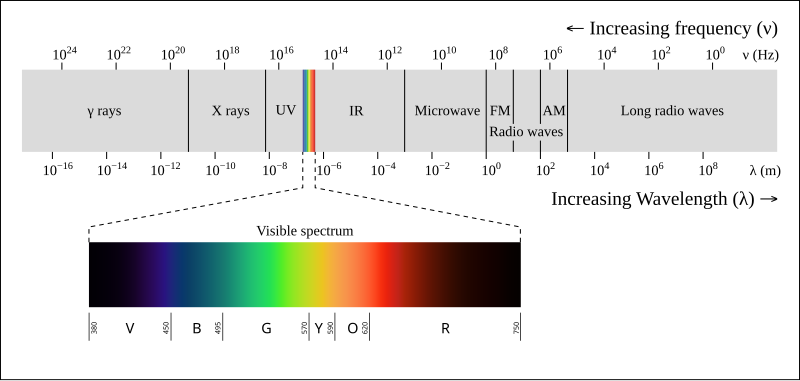
\includegraphics[keepaspectratio]{chapters/images/2_lightspectrum.png}}

Psychologists working in R often use numeric data, and see this as a
list (or vector) of numbers. For example, below is data on the
narcissism (variable = NPI; a measure of how self-absorbed;
self-interested) of a group of Berkeley Haas MBA students
were\footnote{These data come from the hormone\_data.csv file, which
  should be updated to our course page. You'll learn more about how to
  access these data files later in this chapter.}.

\begin{Shaded}
\begin{Highlighting}[]
\NormalTok{haas }\OtherTok{\textless{}{-}} \FunctionTok{read.csv}\NormalTok{(}\StringTok{"./chapter\_data/hormone\_data.csv"}\NormalTok{, }\AttributeTok{stringsAsFactors =}\NormalTok{ T) }
\NormalTok{haas}\SpecialCharTok{$}\NormalTok{NPI}
\end{Highlighting}
\end{Shaded}

\begin{verbatim}
  [1] 3.43 4.40 3.13   NA 3.00   NA 3.05   NA   NA 3.63 3.95 3.08 3.83 3.23 3.80
 [16] 1.80 3.68 3.48 2.73 3.40 2.95 3.65 2.88 2.50 3.13 2.75 3.00 3.15 3.30 3.20
 [31] 2.43 3.13   NA 3.33 2.88 2.55 3.35 3.30 3.28 3.08 2.48 2.78 4.58 2.53 2.78
 [46] 2.88   NA 3.43 2.48 3.50 2.40 3.28 3.63 3.13 2.05 2.98 2.53 3.45 2.80 2.60
 [61] 2.05 2.60 2.73 3.25 2.78 2.93 3.08 3.33 4.05 3.65 3.15 3.33 3.98 4.48 3.00
 [76] 3.00 3.25 4.28 3.13 3.83 3.98 4.13 3.73 3.28 2.85 3.28 3.70 3.03 3.38 2.88
 [91] 3.20 3.40 3.70 3.50 2.58 2.90 3.00 3.35 2.63   NA   NA 4.05 3.43 4.28 3.00
[106] 3.10 3.13 2.83 2.78 2.33 2.68 2.88 2.53 3.80 3.48 3.15 4.38 3.73 3.80 2.60
[121] 3.38 3.13
\end{verbatim}

\textbf{Professor Interpretation} I learn a lot just from this simple
output! \footnote{We'll go over how to load datasets in R in Part 2. For
  this part of the chapter, the focus is on understanding what R is
  doing, and why we are doing it.}

\begin{itemize}
\tightlist
\item
  \textbf{haas \textless-
  read.csv(``./chapter\_data/hormone\_data.csv'', stringsAsFactors =
  T'')} is the R command that loads the dataset. Note that the path to
  the datafile - hormone\_data.csv - is specific to the way I've stored
  these data in my file system. You'll learn below how to change this to
  access your own dataset :)
\item
  \textbf{haas\$NPI} is the R command that was used to generate the
  output below; a list of 122 individual Narcissism scores.

  \begin{itemize}
  \tightlist
  \item
    I know there's 122 individual scores because R is keeping count for
    me using indexing; the numbers in brackets. {[}1{]} shows that the
    first person in the dataset has a narcissism (NPI) score of 3.43;
    {[}118{]} 3.73 shows that this is the score for the 118th person in
    the dataset, and then I can count up to 122. There are much faster
    ways to do this, but I can do it this way too :)
  \item
    I also see there are a few missing data points in the responses -
    these are marked as NA. This could be people who didn't complete the
    survey or were excluded for other reasons (e.g.~missing data).
  \end{itemize}
\end{itemize}

\subsection{Graphing : The Histogram}\label{graphing-the-histogram}

Always always always graph your data. Graphs will help summarize,
organize, and highlight important features of your data that would be
impossible to see just by looking at numbers.\footnote{yes, dear
  student, it is true : a picture is worth\ldots a thousand words.}

\textbf{The Histogram} is a common way researchers illustrate numeric
variables. The histogram organizes data - you lose the individual
values, but gain understanding in seeing how data are grouped together,
which helps you observe patterns and get a quick summary of the
variable.

There are two dimensions of a histogram :

\begin{itemize}
\item
  \textbf{the x-axis} (the horizontal axis; what goes across) : displays
  the values of the variable as organized into groups (or ``breaks'', in
  R).~
\item
  \textbf{the y-axis} (the vertical axis; what goes up and down) :
  displays the frequency (or count) of the individuals in the data who
  ``belong'' to that group.
\end{itemize}

Let's look at our MBA friends again, through the power of a histogram.
As you look at a graph, it's important to practice thinking about what
you learn from the data. Let's avoid fancy stats terminology for now;
it's not necessary for our purposes!!

\begin{Shaded}
\begin{Highlighting}[]
\FunctionTok{hist}\NormalTok{(haas}\SpecialCharTok{$}\NormalTok{NPI, }\AttributeTok{xlab =} \StringTok{"Narcissism Score"}\NormalTok{, }\AttributeTok{col =} \StringTok{\textquotesingle{}black\textquotesingle{}}\NormalTok{, }\AttributeTok{bor =} \StringTok{\textquotesingle{}white\textquotesingle{}}\NormalTok{, }\AttributeTok{main =} \StringTok{""}\NormalTok{)}
\end{Highlighting}
\end{Shaded}

\pandocbounded{\includegraphics[keepaspectratio]{chapters/2R_Data_files/figure-pdf/unnamed-chunk-2-1.pdf}}

\begin{itemize}
\item
  \textbf{the code :} this code draws a histogram using the
  \texttt{hist()} function. I've also added several \texttt{arguments}
  that change some of the default settings to give the graph some
  \emph{digital style.}

  \begin{itemize}
  \item
    \texttt{xlab} gives the x-axis of the graph a nice label.
  \item
    \texttt{col}changes the color of the bars to black.
  \item
    \texttt{bor} changes the color of the lines surrounding the bars to
    white.
  \item
    \texttt{main} changes the title. In this case, \texttt{""} sets the
    title to be nothing, so there's no title.
  \end{itemize}
\item
  \textbf{the graph :} okay, what did R do!

  \begin{itemize}
  \item
    \textbf{x-axis :} this reports the grouped values of the individual
    narcissism scores.~
  \item
    \textbf{y-axis :} this reports how many people were in each group.
  \end{itemize}
\item
  \textbf{professor interpretation with no fancy stats language needed.}

  \begin{itemize}
  \item
    most people (around 42?) had a narcissism score between 3 and 3.5
  \item
    a few people were really high in narcissism\ldots above a 4.5. I'm
    not sure from the graph exactly how many people were in this group,
    or what their score was.
  \item
    a few people were really low in narcissism\ldots below a 2. Again,
    I'm not sure from the graph exactly how many people were in this
    group, or what their score was, but I see their humble selves!
  \item
    I also notice that this is not a super large study - the frequencies
    on the y-axis are relatively low numbers.
  \end{itemize}
\end{itemize}

\subsection{Activity : Think about
Data!}\label{activity-think-about-data}

Okay, your turn. Below is a graph from the same MBA students, but this
time measuring their testosterone levels. Look over the graph, THINK
about what you see, and then expand the textbox below (click on the
arrow on the right side of the green box) to see what I wrote.

\begin{Shaded}
\begin{Highlighting}[]
\FunctionTok{hist}\NormalTok{(haas}\SpecialCharTok{$}\NormalTok{test, }
     \AttributeTok{xlab =} \StringTok{"Testosterone Level"}\NormalTok{, }\AttributeTok{main =} \StringTok{""}\NormalTok{, }
     \AttributeTok{col =} \StringTok{\textquotesingle{}black\textquotesingle{}}\NormalTok{, }\AttributeTok{bor =} \StringTok{\textquotesingle{}white\textquotesingle{}}\NormalTok{)}
\end{Highlighting}
\end{Shaded}

\pandocbounded{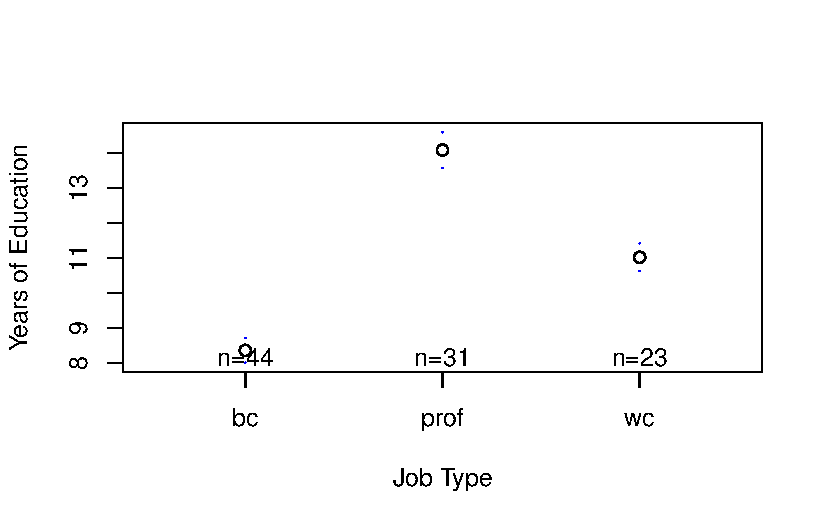
\includegraphics[keepaspectratio]{chapters/2R_Data_files/figure-pdf/unnamed-chunk-3-1.pdf}}

\begin{tcolorbox}[enhanced jigsaw, toptitle=1mm, toprule=.15mm, rightrule=.15mm, breakable, left=2mm, colbacktitle=quarto-callout-tip-color!10!white, colback=white, opacityback=0, coltitle=black, bottomtitle=1mm, opacitybacktitle=0.6, titlerule=0mm, leftrule=.75mm, arc=.35mm, bottomrule=.15mm, title=\textcolor{quarto-callout-tip-color}{\faLightbulb}\hspace{0.5em}{PROFESSOR SPOILERS : Expand this textbox when you are ready by clicking
on the arrow ---\textgreater{}}, colframe=quarto-callout-tip-color-frame]

\begin{itemize}
\tightlist
\item
  \textbf{the graph}

  \begin{itemize}
  \tightlist
  \item
    \textbf{x-axis} : this reports the grouped values of the individual
    testosterone scores, measured in some kind of density (pg/ML)
  \item
    \textbf{y-axis} : this reports how many people were in each group.
  \end{itemize}
\item
  \textbf{what I see and observe with no stats language :}

  \begin{itemize}
  \tightlist
  \item
    most people (around 25+12+20 = 77) had a testosterone level between
    50 and 100.
  \item
    there were no scores below zero (which makes sense) and one person
    who had a very high level of testosterone. I'm not a hormone
    researcher, but the non-negative values seems good, and I might want
    to make sure that there wasn't some data entry error for the extreme
    score.
  \item
    Again, I notice that this is not a super large study\ldots.and these
    relatively low numbers seem similar to the narcissism data, which
    makes sense since they came from the same study.
  \end{itemize}
\end{itemize}

\end{tcolorbox}

\section{Categorical Variable}\label{categorical-variable}

\subsection{Definition : Categorical
Variable}\label{definition-categorical-variable}

A categorical variable is when the values of the variable represent
different groups (or categories). Categories are often useful and simple
ways to group individuals together. For example, when I see a color, I
don't ever describe it in terms of its color hex code or specific
wavelength - I just call it by the simple primary color that I got from
the crayola box\ldots.maybe the 24 color version if I'm feeling fancy.

Which of the shades below would you call blue?\footnote{they are all one
  color - the \emph{human color}. just kidding from the top left it's 2,
  3, 4, and 7. but I'm blue green color blind so you should argue with
  me in the comments.}

\begin{center}

\includegraphics[width=4.04167in,height=\textheight,keepaspectratio]{chapters/images/2_shadesofcyan.png}
\end{center}

The broad label for the variable is called \textbf{the factor}, and the
specific groups of data are called \textbf{levels}. So in the color
example, the category of color would be the factor, and the different
groups of color would be the levels.

As another example, researchers can measure gender with categories such
as female, male, transgender, and other. Identify the factor and levels
in this example.

\begin{tcolorbox}[enhanced jigsaw, toptitle=1mm, toprule=.15mm, rightrule=.15mm, breakable, left=2mm, colbacktitle=quarto-callout-tip-color!10!white, colback=white, opacityback=0, coltitle=black, bottomtitle=1mm, opacitybacktitle=0.6, titlerule=0mm, leftrule=.75mm, arc=.35mm, bottomrule=.15mm, title=\textcolor{quarto-callout-tip-color}{\faLightbulb}\hspace{0.5em}{What are the factors and levels in the example above?}, colframe=quarto-callout-tip-color-frame]

\begin{itemize}
\tightlist
\item
  Factor : would be the variable of gender. Generally there's one factor
  label for each variable.
\item
  Level : would be the categories female, male, transgender, and other.
\end{itemize}

\end{tcolorbox}

\subsection{Culture in Statistics : Gender
Identity}\label{culture-in-statistics-gender-identity}

\marginnote{\begin{footnotesize}

\includegraphics[width=1.625in,height=\textheight,keepaspectratio]{images/doff_intro_mickey.png}

\textsc{Hi folks! It's me again, Open-Source Mickey Mouse to talk with
you about the idea that statistics has a culture that is socially
constructed by people like you!}

\end{footnotesize}}

\textsc{One domain where this is particularly relevant is in the area of
gender identity. While many people identify as ``male'' or ``female'',
some people don't fit into these categories. (Seems pretty simple to me
to let folks exist as they want! But I'm just a poor open-source servant
freed from my corporate overlords.) Yet as folks in power have recently
forced this narrow binary view of gender identity onto everyone, it
becomes even more critical to engage with these ideas and try to define
a science that can capture the complexity of human life in ways that let
people be their full selves.}

\textsc{Unfortunately, most psychological researchers still hold on to
Male / Female binaries in the way they measure gender or sex, yet there
are many reasons - both scientific and humanistic - to give people more
range to express important aspects of their identity.}

\begin{figure}[H]

{\centering \pandocbounded{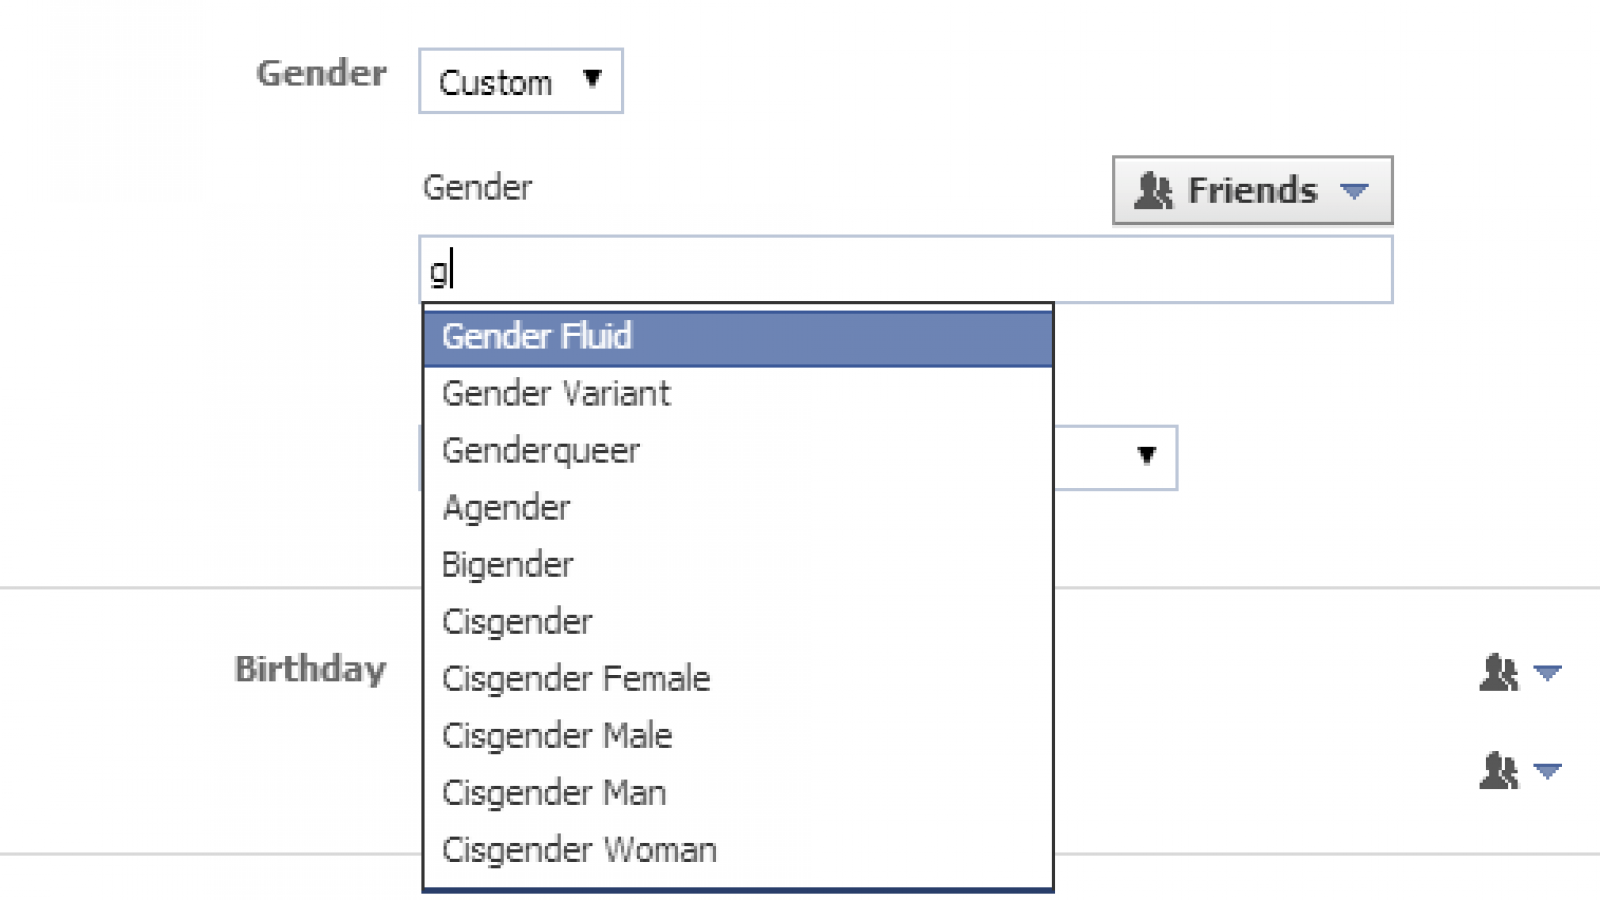
\includegraphics[keepaspectratio]{chapters/images/2_fb_gender.png}}

}

\caption{\href{http://abcnews.go.com/blogs/headlines/2014/02/heres-a-list-of-58-gender-options-for-facebook-users}{facebook's
attempt} at measuring more complex categories.}

\end{figure}%

\textsc{Indeed, categories almost always oversimplify the complexity of
life, yet are often used by people (and researchers) because they can
sometimes be useful and simple shortcuts for us to understand the
world.}

\textsc{If you are simply interested in doing a superficial survey of a
variable like race, ethnicity, or gender, then I think categorical data
can be a fine -if often unscientific - approach, and would recommend
giving all people the chance to express their identity in some way. For
example,
\href{https://compass.onlinelibrary.wiley.com/doi/pdfdirect/10.1111/spc3.12506}{here's
an article} describing research on the way that exclusionary categories
can negatively impact science, and offering clear and easy
recommendations for reseachers to broaden science (e.g., reporting
non-binary participants).}

\textsc{However, if you are interested in really digging into a
variable, then a continuous approach is almost always best, since it
allows for more flexibility in capturing complexity in variation. We'll
discuss more on how to do this in a few weeks when we learn about
measuring continuous variables with likert scales.}

\pandocbounded{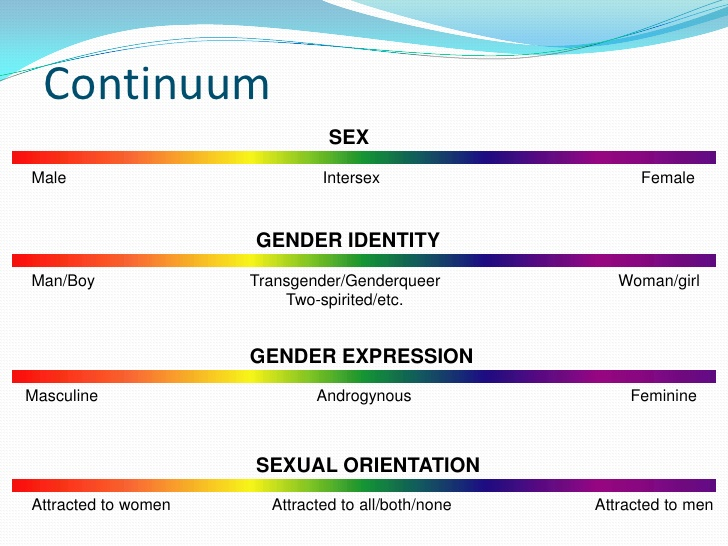
\includegraphics[keepaspectratio]{chapters/images/2_genderspectrum.png}}\footnote{a
  \href{https://scalar.usc.edu/works/index-2/media/the-gender-spectrum}{continuous
  approach} to measuring gender. hi if u still reading, let me know if
  you have any thoughts on this section of the chapter.}

\subsection{Graphing : The Categorical
Plot}\label{graphing-the-categorical-plot}

The histogram only describes a graph for numeric data, since it
organizes numbers into groups (it kind of turns complex variation into
more simple categories). When the variable is categorical, people call
it a plot 🤷.

This graph looks very similar to our histogram :~

\begin{itemize}
\item
  \textbf{the x-axis} (the horizontal axis; what goes across) : displays
  the levels of the factor variable.
\item
  \textbf{the y-axis} (the vertical axis; what goes up and down) :
  displays the frequency (or count) of the individuals in the data who
  ``belong'' to each group.
\end{itemize}

Alright, back to our good MBA friends. This is a graph of the
categorical variable ``sex''. Again, look over the graph, THINK about
what you see (no stats terminology; what do you learn!), and then
highlight my text to see what I wrote about.

\begin{Shaded}
\begin{Highlighting}[]
\FunctionTok{plot}\NormalTok{(haas}\SpecialCharTok{$}\NormalTok{sex, }\AttributeTok{col =} \StringTok{\textquotesingle{}black\textquotesingle{}}\NormalTok{, }\AttributeTok{bor =} \StringTok{\textquotesingle{}white\textquotesingle{}}\NormalTok{, }\AttributeTok{xlab =} \StringTok{"Sex"}\NormalTok{)}
\end{Highlighting}
\end{Shaded}

\pandocbounded{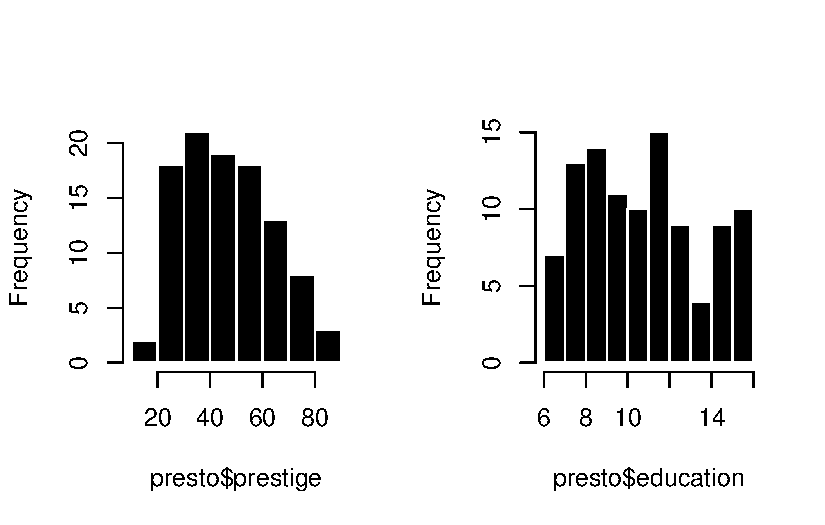
\includegraphics[keepaspectratio]{chapters/2R_Data_files/figure-pdf/unnamed-chunk-4-1.pdf}}

\begin{itemize}
\item
  \textbf{The Code :} this code draws a histogram using the
  \texttt{plot()} function. Note that I've asked R to \texttt{plot} the
  variable \texttt{haas\$sex}. I've also added several
  \texttt{arguments} that change some of the default settings to give
  the graph some \emph{digital style.}

  \begin{itemize}
  \item
    \texttt{xlab} gives the x-axis of the graph a nice label.
  \item
    \texttt{col}changes the color of the bars to black.
  \item
    \texttt{bor} changes the color of the lines surrounding the bars to
    white.
  \end{itemize}
\item
  \textbf{The Graph :}

  \begin{itemize}
  \item
    \textbf{x-axis :} this reports levels (female; male) of the
    categorical factor variable Sex.~
  \item
    \textbf{y-axis :} this reports how many people were in each group.
  \end{itemize}
\item
  \textbf{What I see and observe with no stats language :}

  \begin{itemize}
  \item
    It appears that the researchers only measured sex as a f/m binary
    (or that no participants reported a category other than female or
    male).
  \item
    there were more males than females in this dataset. This matches my
    perception / stereotype of what a typical MBA program might look
    like; however I looked into it and Haas reports a larger percentage
    of female enrollments in the MBA program; so our data may not serve
    as a representative sample of the true population.\footnote{Will
      learn about these ideas much later this semester! here's a link to
      learn more about
      \href{https://mba.haas.berkeley.edu/student-life/women}{women in
      Haas}. capitalism will eat us all eventually I guess, and good to
      challenge our stereotypes / perceptions!}\\
  \end{itemize}
\end{itemize}

\chapter{Part 2 : Data and Datasets in
R}\label{part-2-data-and-datasets-in-r}

\section{Defining Variables in R}\label{defining-variables-in-r}

Below are some videos, and R code, that review how to define a variable
in R. Yeah! I'm not going to share the Rscripts I'm using for these
videos, since I think there's value in typing this out yourself to get
that muscle memory in 💪🤘 but let me know if you disagree / there's a
reason to provide them to y'all!

\subsection{Video : Defining Numeric Variables in
R}\label{video-defining-numeric-variables-in-r}

\url{https://youtu.be/0pXGqGDSySM}

\begin{itemize}
\item
  objects - assign function for numerical data
\item
  c() : combining data together.
\item
  length() : the number of objects
\end{itemize}

\subsection{Video : Graphing Numeric Variables in
R}\label{video-graphing-numeric-variables-in-r}

\url{https://youtu.be/lmXQ2BhQNuo}

\begin{itemize}
\item
  hist() : a graph
\item
  changing arguments : xlab, ylab, main
\end{itemize}

\subsection{Video : Defining Categorical Variables in
R}\label{video-defining-categorical-variables-in-r}

\url{https://youtu.be/CFXRxfaadIw}

\begin{itemize}
\tightlist
\item
  categorical data (``string'')
\item
  as.factor() : to convert a string to a categorical variable
\item
  levels() : to see the levels of your categorical variable.
\end{itemize}

\subsection{Video : Graphing categorical variables in
R}\label{video-graphing-categorical-variables-in-r}

\url{https://youtu.be/Fmai9Ltpa5I}

\begin{itemize}
\tightlist
\item
  plot()
\item
  changing arguments : col, bor, main; xlab; ylab
\end{itemize}

\section{The Dataframe}\label{the-dataframe}

\subsection{Definition : Rows and
Columns}\label{definition-rows-and-columns}

As a researcher, you'll be interested in understanding not only one
variable at a time, but will be interested in a dataset - multiple
variables about an individual that are organized - in order to see how
variables are related to each other (remember : this is a function of
the linear model).

The datasets in our class will be stored on Dropbox; you can find a link
to this on our course page, under the Course Materials module (see below
for the image that you're looking for).

\begin{center}
\pandocbounded{
\includegraphics[keepaspectratio]{chapters/images/2_dropboxchapters.png}}
\end{center}

You'll learn how to load these datasets later in this lecture. For now,
what is a dataset?

A dataset is really a \textbf{dataframe} - a two-dimensional way to
organize data - and takes the following structure in this class.

\begin{itemize}
\item
  \textbf{the rows} define the individual in the dataset.~rows go across
  horizontally, like a rowboat going across a lake.
\item
  the columns define the variables in the dataset. ~go up and down
  vertically; like what might support a bridge.
\end{itemize}

Look at the example below - again from our budding MBAs in the Haas
program. What do you observe about the rows and columns? What does this
tell you about the dataset?

\textbf{\pandocbounded{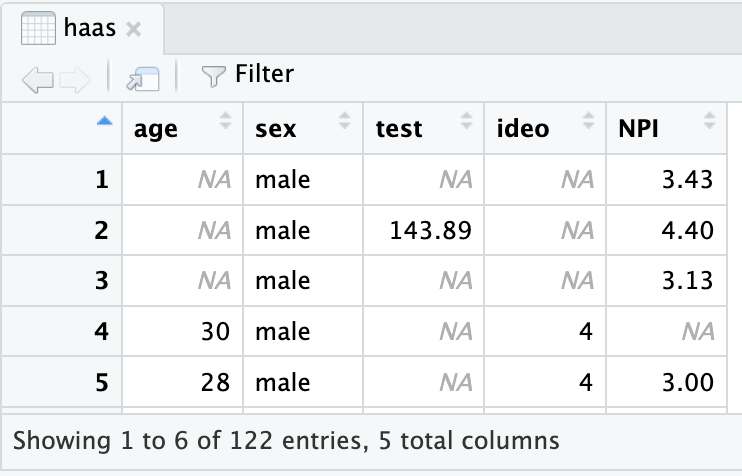
\includegraphics[keepaspectratio]{chapters/images/2_haas_dataframe.png}}}\\
\strut \\
In the example dataframe above - I see 5 rows (representing 5
individuals) and five columns (representing five variables like the
person's \textbf{age}, their \textbf{sex,} their \textbf{test}osterone
levels, political \textbf{ideo}logy, and their \textbf{NPI} (Narcissism)
score.~ or their Race, etc.) Note that the names of the variables do not
count as a row, since these are not individuals in the dataset, and you
would need to know more about the dataset to know that ideo = political
ideology, or test = testosterone. I also see that R is helpfully telling
me that this is only a snapshot of the entire dataset - the whole
dataframe has 122 entries (rows), meaning that there's 122 MBA students
in this dataset, and 5 total columns (which we can all see here.)

As a researcher, you have access to an entire dataset (either collected
by you or another researcher) that organizes multiple variables for each
individual. This semester, we'll work with a variety of datasets on
different psychological topics - not just haas students.

\subsection{Definition : Indexing}\label{definition-indexing}

The dataset gives us access to all the individual rows and columns at
once, we will often want to focus on one specific variable (or
individual) at a time. \textbf{Indexing} refers to a flexible method of
selecting a specific set of data from a larger collection. Previously'
we've seen indexing when asking R to produce a large set of numbers; for
example asking it to count from 1 to 100.

\begin{Shaded}
\begin{Highlighting}[]
\DecValTok{1}\SpecialCharTok{:}\DecValTok{100}
\end{Highlighting}
\end{Shaded}

\begin{verbatim}
  [1]   1   2   3   4   5   6   7   8   9  10  11  12  13  14  15  16  17  18
 [19]  19  20  21  22  23  24  25  26  27  28  29  30  31  32  33  34  35  36
 [37]  37  38  39  40  41  42  43  44  45  46  47  48  49  50  51  52  53  54
 [55]  55  56  57  58  59  60  61  62  63  64  65  66  67  68  69  70  71  72
 [73]  73  74  75  76  77  78  79  80  81  82  83  84  85  86  87  88  89  90
 [91]  91  92  93  94  95  96  97  98  99 100
\end{verbatim}

The indexing shows up as brackets next to the actual data, and is way
for R to index that the {[}1{]}st data entry is the number 1, the
{[}24{]}th entry is the number 24, and so on.

When I ask R to show me the dataset haas, the output can be
overwhelming. Below is what R shows you when you ask to see the haas
dataset. And this is a relatively small dataset with just 122
individuals (rows) and five variables (columns).

\begin{Shaded}
\begin{Highlighting}[]
\NormalTok{haas}
\end{Highlighting}
\end{Shaded}

\begin{verbatim}
    age    sex   test ideo  NPI
1    NA   male     NA   NA 3.43
2    NA   male 143.89   NA 4.40
3    NA   male     NA   NA 3.13
4    30   male     NA    4   NA
5    28   male     NA    4 3.00
6    33 female     NA    5   NA
7    NA   male     NA   NA 3.05
8    NA   male     NA   NA   NA
9    NA   male  77.95   NA   NA
10   NA   male     NA   NA 3.63
11   26   male 126.29    3 3.95
12   31   male  59.48    5 3.08
13   27   male  89.45    4 3.83
14   27   male  82.80    3 3.23
15   28   male  97.39    4 3.80
16   30   male  54.80    4 1.80
17   28   male  46.07    4 3.68
18   24   male     NA    4 3.48
19   32   male  87.40    3 2.73
20   25   male  85.01    4 3.40
21   27   male     NA    3 2.95
22   25   male     NA    4 3.65
23   24   male 102.86    3 2.88
24   28   male  73.60    3 2.50
25   27   male     NA    2 3.13
26   29   male  90.68    4 2.75
27   28   male  44.70    3 3.00
28   29   male     NA    4 3.15
29   30   male  77.61    4 3.30
30   26   male  57.20    5 3.20
31   31   male  49.92    4 2.43
32   28   male     NA    3 3.13
33   32   male     NA    5   NA
34   27   male  85.01    2 3.33
35   32   male  74.86    2 2.88
36   27   male 125.89    3 2.55
37   29   male  77.07    4 3.35
38   30   male     NA    4 3.30
39   26   male  30.54    4 3.28
40   27   male  73.76    3 3.08
41   32   male  65.61    3 2.48
42   29   male  51.23    4 2.78
43   28   male  85.17    3 4.58
44   28   male     NA    3 2.53
45   29   male  57.14    2 2.78
46   30   male  65.31    4 2.88
47   28   male  53.07    4   NA
48   28   male 104.65    3 3.43
49   31   male  90.32    3 2.48
50   NA female  24.71   NA 3.50
51   26 female  20.99    3 2.40
52   27 female     NA    4 3.28
53   28 female     NA    3 3.63
54   28 female   5.51    5 3.13
55   27 female  40.49    4 2.05
56   25 female  35.05    2 2.98
57   26 female  57.71    4 2.53
58   26 female  27.36    4 3.45
59   27 female  59.37    3 2.80
60   26 female  21.63    3 2.60
61   29 female     NA    3 2.05
62   25 female     NA    7 2.60
63   37 female  39.50    4 2.73
64   28 female  42.35    4 3.25
65   24 female  32.42    3 2.78
66   29   male  97.63    4 2.93
67   28   male 131.51    3 3.08
68   26   male     NA    4 3.33
69   27   male     NA    5 4.05
70   29   male     NA    2 3.65
71   27   male 140.53    2 3.15
72   26   male     NA    3 3.33
73   28   male     NA    3 3.98
74   22   male  90.88    5 4.48
75   29   male 148.24    5 3.00
76   29   male 132.24    4 3.00
77   27   male  82.43    4 3.25
78   26   male  73.43    4 4.28
79   35   male     NA    2 3.13
80   27   male 100.49    4 3.83
81   25   male  94.31    4 3.98
82   27   male  72.53    2 4.13
83   30   male 133.35    4 3.73
84   27   male  59.77    4 3.28
85   30   male  91.83    4 2.85
86   29   male  82.13    3 3.28
87   30   male 172.15    3 3.70
88   29   male 228.17    2 3.03
89   27   male 133.70    3 3.38
90   27   male  89.24    4 2.88
91   28   male  88.62    3 3.20
92   28   male  86.83    4 3.40
93   25   male 138.65    4 3.70
94   33   male  59.75    4 3.50
95   28   male  46.30    3 2.58
96   31   male 107.02    3 2.90
97   24   male  60.16    2 3.00
98   26   male     NA    4 3.35
99   27   male 107.71    3 2.63
100  23   male  99.64    2   NA
101  32   male 131.51    3   NA
102  29   male  91.94    4 4.05
103  25   male  53.67    3 3.43
104  25   male     NA    4 4.28
105  27 female     NA    4 3.00
106  27 female  59.24    2 3.10
107  30 female  28.03    5 3.13
108  28 female  33.38    5 2.83
109  26 female  53.31    4 2.78
110  28 female  27.53    4 2.33
111  29 female  16.89    4 2.68
112  25 female  51.53    4 2.88
113  26 female  37.15    4 2.53
114  27 female  50.55    2 3.80
115  28 female     NA    4 3.48
116  28 female  41.35    5 3.15
117  29 female  64.66    5 4.38
118  24 female  37.95    2 3.73
119  27 female  54.26    4 3.80
120  27 female     NA    4 2.60
121  27 female 113.41    4 3.38
122  29 female  41.35    3 3.13
\end{verbatim}

I am overwhelmed with data. So it will be important to find ways to
target the data that we want. There are several ways we can do this!

Because a dataset has two different dimensions, we have to use two
coordinates to index the dataset - one coordinate for the row(s) that we
want to focus on, and one coordinate for the column(s) that we want to
focus on.\\

\subsubsection{Indexing an Entire
Dataset}\label{indexing-an-entire-dataset}

Because a dataset has two different dimensions, we have to use two
coordinates to index the dataset - one coordinate for the row(s) that we
want to focus on, and one coordinate for the column(s) that we want to
focus on.

\begin{itemize}
\item
  \texttt{data} \# this reports the entire dataset. In the example to
  the right, I've typed in haas (since this is the name of the dataset
  in this example) and see the dataset reported.
\item
  \texttt{data{[}i,\ j{]}} \# this code returns a specific row (i), and
  a specific column (j). The convention is to use the letter i for a row
  first, then j for a column \textbf{{[}you can remember this order as
  RC Car, or R is Cool{]}.} For example

\begin{Shaded}
\begin{Highlighting}[]
\NormalTok{haas[}\DecValTok{2}\NormalTok{,}\DecValTok{3}\NormalTok{]}
\end{Highlighting}
\end{Shaded}

\begin{verbatim}
[1] 143.89
\end{verbatim}

  Shows me that R has highlighted the second row and third column of the
  dataset - the second person's testosterone level is 143.89 units.
\item
  \texttt{data{[}\ ,\ j{]}} \# if you leave a blank for the rows, then R
  will return all of the rows, and whatever column you specify. This can
  be good for looking at a specific variable for all individuals. For
  example, the following code returns all of the testosterone data (the
  third column).
\end{itemize}

\begin{Shaded}
\begin{Highlighting}[]
\InformationTok{\textasciigrave{}\textasciigrave{}\textasciigrave{}\{r\}}
\InformationTok{haas[,3]}
\InformationTok{\textasciigrave{}\textasciigrave{}\textasciigrave{}}
\end{Highlighting}
\end{Shaded}

\begin{itemize}
\item
  \texttt{data{[}i,\ {]}} \# ~if you leave a blank for the column, then
  you would see all of the columns for a specific row. This can be good
  for looking at a specific individual's entire dataset; such as all of
  participant 2's data below.

\begin{Shaded}
\begin{Highlighting}[]
\NormalTok{haas[}\DecValTok{2}\NormalTok{,]}
\end{Highlighting}
\end{Shaded}

\begin{verbatim}
  age  sex   test ideo NPI
2  NA male 143.89   NA 4.4
\end{verbatim}
\item
  \texttt{haas{[}i:i,\ c(j,\ j){]}} \# you can adapt this code to give a
  range of values too. for example, if I want to see rows 4-10 and
  columns 1 and 3, I would run the following code.

\begin{Shaded}
\begin{Highlighting}[]
\NormalTok{haas[}\DecValTok{4}\SpecialCharTok{:}\DecValTok{10}\NormalTok{, }\FunctionTok{c}\NormalTok{(}\DecValTok{1}\NormalTok{,}\DecValTok{3}\NormalTok{)]}
\end{Highlighting}
\end{Shaded}

\begin{verbatim}
   age  test
4   30    NA
5   28    NA
6   33    NA
7   NA    NA
8   NA    NA
9   NA 77.95
10  NA    NA
\end{verbatim}
\end{itemize}

\subsubsection{Indexing a Single
Variable}\label{indexing-a-single-variable}

\begin{itemize}
\item
  \texttt{data\$variable} \# You can also use the \$ (dollar sign) in R
  to reference a single variable from a dataset. This is very useful,
  because you can use the name of the variable instead of the numerical
  index. So, for example, if I want to highlight the testosterone levels
  of the haas dataset, I would run the following :

\begin{Shaded}
\begin{Highlighting}[]
\NormalTok{haas}\SpecialCharTok{$}\NormalTok{test}
\end{Highlighting}
\end{Shaded}

\begin{verbatim}
  [1]     NA 143.89     NA     NA     NA     NA     NA     NA  77.95     NA
 [11] 126.29  59.48  89.45  82.80  97.39  54.80  46.07     NA  87.40  85.01
 [21]     NA     NA 102.86  73.60     NA  90.68  44.70     NA  77.61  57.20
 [31]  49.92     NA     NA  85.01  74.86 125.89  77.07     NA  30.54  73.76
 [41]  65.61  51.23  85.17     NA  57.14  65.31  53.07 104.65  90.32  24.71
 [51]  20.99     NA     NA   5.51  40.49  35.05  57.71  27.36  59.37  21.63
 [61]     NA     NA  39.50  42.35  32.42  97.63 131.51     NA     NA     NA
 [71] 140.53     NA     NA  90.88 148.24 132.24  82.43  73.43     NA 100.49
 [81]  94.31  72.53 133.35  59.77  91.83  82.13 172.15 228.17 133.70  89.24
 [91]  88.62  86.83 138.65  59.75  46.30 107.02  60.16     NA 107.71  99.64
[101] 131.51  91.94  53.67     NA     NA  59.24  28.03  33.38  53.31  27.53
[111]  16.89  51.53  37.15  50.55     NA  41.35  64.66  37.95  54.26     NA
[121] 113.41  41.35
\end{verbatim}
\item
  \texttt{data\$variable{[}i{]}} \# We can then use indexing to narrow
  this down. Because a variable only has one dimension (it's just a
  collection of individuals; not rows and individuals) I only need to
  use one coordinate to index the specific individual(s) I want to find.
\end{itemize}

\begin{Shaded}
\begin{Highlighting}[]
\NormalTok{haas}\SpecialCharTok{$}\NormalTok{test[}\DecValTok{2}\NormalTok{]}
\end{Highlighting}
\end{Shaded}

\begin{verbatim}
[1] 143.89
\end{verbatim}

\begin{itemize}
\item
  \texttt{data\$variable{[}i:i{]}} \# Can be used to find a range of
  individuals. These numbers need to be sequential for this code to
  work.

\begin{Shaded}
\begin{Highlighting}[]
\NormalTok{haas}\SpecialCharTok{$}\NormalTok{test[}\DecValTok{1}\SpecialCharTok{:}\DecValTok{3}\NormalTok{]}
\end{Highlighting}
\end{Shaded}

\begin{verbatim}
[1]     NA 143.89     NA
\end{verbatim}
\item
  \texttt{data\$variable{[}c(i,i,i){]}} \# If you want to find
  individuals who are not next to each other, you need to use the
  \textbf{c (combine) function} to combine multiple coordinates
  together. You can have as many coordinates here as you want. For
  example :~

\begin{Shaded}
\begin{Highlighting}[]
\NormalTok{haas}\SpecialCharTok{$}\NormalTok{test[}\FunctionTok{c}\NormalTok{(}\DecValTok{2}\NormalTok{,}\DecValTok{3}\NormalTok{,}\DecValTok{14}\SpecialCharTok{:}\DecValTok{18}\NormalTok{, }\DecValTok{116}\SpecialCharTok{:}\DecValTok{118}\NormalTok{)]}
\end{Highlighting}
\end{Shaded}

\begin{verbatim}
 [1] 143.89     NA  82.80  97.39  54.80  46.07     NA  41.35  64.66  37.95
\end{verbatim}
\end{itemize}

\subsubsection{Test Yourself : Indexing!}\label{test-yourself-indexing}

Okay, practice time. Use the haas dataset and your knowledge of indexing
to identify what R would show if you typed in the following commands (no
R required)

\begin{itemize}
\tightlist
\item
  haas\$age{[}47{]}
\item
  haas\$NPI{[}1:3{]}
\item
  haas{[}51,2{]}
\item
  haas{[}60, {]}
\item
  haas{[} , 6{]}
\end{itemize}

\begin{tcolorbox}[enhanced jigsaw, toptitle=1mm, toprule=.15mm, rightrule=.15mm, breakable, left=2mm, colbacktitle=quarto-callout-tip-color!10!white, colback=white, opacityback=0, coltitle=black, bottomtitle=1mm, opacitybacktitle=0.6, titlerule=0mm, leftrule=.75mm, arc=.35mm, bottomrule=.15mm, title=\textcolor{quarto-callout-tip-color}{\faLightbulb}\hspace{0.5em}{Answer Key : Indexing!}, colframe=quarto-callout-tip-color-frame]

\begin{itemize}
\tightlist
\item
  28
\item
  3.43 4.40 3.13
\item
  female
\item
  26 female 21.63 3 2.6
\item
  you would get an error; there is no 6th column.
\end{itemize}

\end{tcolorbox}

\subsection{In R : How to Navigate
Datasets}\label{in-r-how-to-navigate-datasets}

Let's get some more practice with some actual data. Before we learn how
to import data in R, we can work with a super exciting dataset that is
already part of the R program - a dataset on the weights of chickens
(chkwt).

Watch the two videos below to see how I navigate this dataset; here's a
\href{https://www.dropbox.com/scl/fi/e9l24v1vshdjih7rctxcn/navigating_data.R?rlkey=st0f3hzkrkmha4u4224f6n43i&dl=0}{link
to the RScript} that I use in the videos.~

\subsubsection{Video : Checking Datasets in
R}\label{video-checking-datasets-in-r}

\url{https://youtu.be/TaonMS3b0pU}

\begin{itemize}
\item
  \textbf{length() :} counts the number of objects (variables) in a
  dataset (or any object)
\item
  \textbf{nrow() :} counts the number of rows (participants) in a
  dataset
\end{itemize}

\textbf{head() :} looks at the first six rows of a dataset

\subsubsection{Video : Navigating Datasets with
Indexing}\label{video-navigating-datasets-with-indexing}

\url{https://youtu.be/js2vV5P4DSQ}

\begin{itemize}
\tightlist
\item
  Use this video to answer the check-in questions below.
\end{itemize}

\subsubsection{\texorpdfstring{\href{https://docs.google.com/forms/d/e/1FAIpQLSeYROuiCU1wKb5W36k9IQIKMra2y5Wt9P84Er8WdBaQ6hvHNw/viewform?usp=sf_link}{Check-In
: Navigating Variables and Datasets with
Indexing}}{Check-In : Navigating Variables and Datasets with Indexing}}\label{check-in-navigating-variables-and-datasets-with-indexing}

Use the fake dataset below and your knowledge of navigating datasets
with indexing to identify what answer R would give if you gave it the
following code. (Note : no R is needed to complete this problem).

\begin{Shaded}
\begin{Highlighting}[]
\NormalTok{data}
\end{Highlighting}
\end{Shaded}

\begin{verbatim}
  StudentID favDrink age
1         1     boba  20
2         2     boba  19
3         3     boba  54
4         4   coffee  22
5         5    water  38
\end{verbatim}

\section{The .csv File}\label{the-.csv-file}

\subsection{Definition : The .csv File}\label{definition-the-.csv-file}

As a researcher, you will work with data that you (or other researcher
friends) have collected. The .csv file (csv stands for comma separated
variables) is one of the most common formats for storing data that you
will encounter. You've probably encountered this before, and likely have
opened this file type in a program like excel or google sheets. But in
this class, we'll learn to load these files directly into R. Using R has
two advantages :

\begin{itemize}
\tightlist
\item
  R is way more powerful than excel or Google Sheets.
\item
  R allows us to document all of our steps. This semester, we'll learn
  how to make changes to the dataset (e.g., changing the names of a
  variable; removing bad data; transforming data). It's important to be
  completely transparent about these changes, and doing these changes in
  R (with an R Script!) will ensure that we document our steps for our
  future selves / other researchers.
\end{itemize}

\subsection{Videos : How to Load Datasets in
R}\label{videos-how-to-load-datasets-in-r}

There are two different ways to load a data file into R : one way (``the
point and click method'') involves clicking some boxes, like most of
y'all are used to doing. The second way involves typing in an R command.
Below are videos that highlight each method.

\begin{tcolorbox}[enhanced jigsaw, toptitle=1mm, toprule=.15mm, rightrule=.15mm, breakable, left=2mm, colbacktitle=quarto-callout-important-color!10!white, colback=white, opacityback=0, coltitle=black, bottomtitle=1mm, opacitybacktitle=0.6, titlerule=0mm, leftrule=.75mm, arc=.35mm, bottomrule=.15mm, title=\textcolor{quarto-callout-important-color}{\faExclamation}\hspace{0.5em}{Important}, colframe=quarto-callout-important-color-frame]

Regardless of which method you use, there are three things you want to
check every time you load data : change the name of the dataset (to make
it something simple to type and memorable); check the headers (make sure
the variables have names, since sometimes), and set stringAsFactors =
TRUE (which will automatically convert all your string variables into
categorical factor variables, which is almost always what you will want
to do in this class.

These instructions are highlighted because students often forget. So
note the importance! They are important steps!!!

\end{tcolorbox}

\subsubsection{Video : Importing Data with the ``Point and Click''
Method and Console
Method}\label{video-importing-data-with-the-point-and-click-method-and-console-method}

\url{https://youtu.be/XLew6OeYAm0}

\begin{itemize}
\tightlist
\item
  the ``point and click'' method of loading data
\item
  the console / Rscript method of loading data
\end{itemize}

\subsubsection{Video : For Posit Users : working with projects and
loading data in the
cloud.}\label{video-for-posit-users-working-with-projects-and-loading-data-in-the-cloud.}

\url{https://youtu.be/HOhINtpyjT4}

\begin{itemize}
\tightlist
\item
  posit.cloud users! You will need an extra step that folks using
  posit.cloud have to use to upload datasets to the cloud (and then
  import them).
\end{itemize}

\section{Practice Quiz 2}\label{practice-quiz-2}

Okay, this was a LOT. Like drinking water from a fire hose. I promise
this will get easier, and it just requires practice. Let's see how clear
the professor's instructions were with this\ldots practice quiz!

\href{https://docs.google.com/forms/d/e/1FAIpQLSczCIkUMPcHX36bYbBpU4fH2Ei_U4neGsERl5WD8jTWRSxfiw/viewform?usp=sf_link}{\textbf{CLICK
THIS LINK to take the Practice Quiz.}} Use your knowledge of navigating
and loading datasets to answer~

\begin{itemize}
\item
  \href{https://www.dropbox.com/scl/fi/972y9dq8yan2l2q7cme5f/2.1_NavigatingData.R?rlkey=al8gff6iqxj0fdiy0mn8wiyp9&dl=0}{\textbf{Here's
  an Rscript with the practice quiz questions}}\textbf{.} Submit your
  answers to the link above for credit (this is graded based on
  completion).
\item
  \href{https://youtu.be/cfeogtcAhNM}{\textbf{Here's a video key with
  the practice quiz answers}}\textbf{.} Please attempt the quiz on your
  own; if you get stuck, refer to the relevant videos above. And feel
  free to reach out on Discord if something's confusing or I got
  something wrong. Appreciate y'alls engagement!
\end{itemize}

\chapter{Part 3 : No Research Methods Stuff This
Week}\label{part-3-no-research-methods-stuff-this-week}

Loading data is a major pain point, so best to focus on that. It will
get easier, I promise :)

\chapter{TLDR}\label{tldr}

We learned about different kinds of data (numeric and categorical), and
how to graph and interpret these data. We also learned how to load and
navigate datasets in R in order to look at variables.

In lecture this week, we will continue to get practice working with
datasets and variables. Yeah!

That is all. Thx for reading, as always.

\chapter{Description}\label{description}

Hello! This week, you'll learn how to use statistics to describe data in
terms of centrality and complexity (and review how the mean and standard
deviation can be thought of as prediction and error).

\begin{center}
\pandocbounded{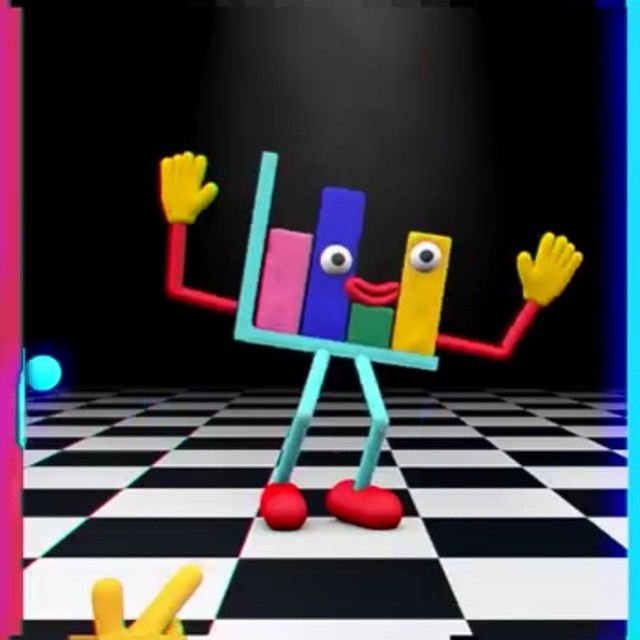
\includegraphics[keepaspectratio]{chapters/images/3_Bar_GraphDigitalStyle.png.webp}}
\end{center}

\begin{tcolorbox}[enhanced jigsaw, toptitle=1mm, toprule=.15mm, rightrule=.15mm, breakable, left=2mm, colbacktitle=quarto-callout-important-color!10!white, colback=white, opacityback=0, coltitle=black, bottomtitle=1mm, opacitybacktitle=0.6, titlerule=0mm, leftrule=.75mm, arc=.35mm, bottomrule=.15mm, title=\textcolor{quarto-callout-important-color}{\faExclamation}\hspace{0.5em}{To-Do List:}, colframe=quarto-callout-important-color-frame]

\begin{itemize}
\tightlist
\item
  Read this document and watch the videos. Are you pressed for time?
  Some guidance below.

  \begin{itemize}
  \tightlist
  \item
    Part 1 : Focus on the mean, and why it's important, and watch the
    videos on standard deviation.
  \item
    Part 2 : Complete the practice quiz and watch the video key. If
    time, watch the video on removing outliers.
  \end{itemize}
\item
  Take Quiz 3 : on using your knowledge of R (and standard deviation) to
  describe data.
\end{itemize}

\end{tcolorbox}

\chapter{Part 1 : Descriptive
Statistics}\label{part-1-descriptive-statistics}

We use statistics as a language to describe how individuals are both
similar to, and different from, each other.

\section{Centrality}\label{centrality}

Statistics like the mean, median, and mode focus on what is most central
to a distribution of data. These measures of centrality reduce the
complexity of individual scores, but in doing so emphasize some of the
core aspects of the variable. You can think of \emph{centrality} like a
summary of the data. While a lot of information is lost in summary
(e.g., Lord of the Rings is much more about some Hobbits trying to
destroy an evil ring), a summary often gets the key points across in few
words (e.g., Lord of the Rings does spend a lot of time describing
Hobbits trying to destroy an evil ring.)

\subsection{The Mean}\label{the-mean}

\subsubsection{Definition.}\label{definition.}

The mean (also known as the average) is one of the most important
statistics, and the foundation for much of what we will do in this
class.

You probably learned this equation as something like, ``add up all the
numbers and divide by the total number of numbers''. This is technically
correct, but scientists like to be more specific and formal, and so
statistics uses a more specific language.

The statistical equation for the mean is below; it may look confusing,
but it is really just a fancy version of the same definition of the mean
you know and love. Specifically, the formula defines the mean as ``equal
to the sum of all individual x-values (starting with the first
individual and ending with the last individual in the dataset), and
divided by the sample size.''

\begin{longtable}[]{@{}
  >{\raggedright\arraybackslash}p{(\linewidth - 2\tabcolsep) * \real{0.2614}}
  >{\raggedright\arraybackslash}p{(\linewidth - 2\tabcolsep) * \real{0.7386}}@{}}
\toprule\noalign{}
\begin{minipage}[b]{\linewidth}\raggedright
The Equation
\end{minipage} & \begin{minipage}[b]{\linewidth}\raggedright
Breakdown of Terminology
\end{minipage} \\
\midrule\noalign{}
\endhead
\bottomrule\noalign{}
\endlastfoot
\(
\Large \bar{y} = \frac{\sum_{i=1}^n y_i}{n}
\) & \begin{minipage}[t]{\linewidth}\raggedright
\begin{itemize}
\tightlist
\item
  \(\bar{y}\) = ``y bar'' = the mean of y
\item
  \(\Sigma\) = Sigma = the ``sum'' of numbers (starting from the number
  on the bottom all the way through the number on the top).
\item
  \(i\) = index = an individual
\item
  \(n\) = sample size = the number of individuals in the dataset
\item
  \(y\) = a variable
\end{itemize}
\end{minipage} \\
\end{longtable}

So, when reading this formula, you would ``say'' : ``y bar (the mean) is
equal to the sum of all individuals of y (\(y_i\)) starting with the
first (\(i=1\)) and going all the way through the total number of
individuals (\(n\)). And then you take that sum, and divide by the total
number of individuals (\(n\)).

See?! Simple!

\subsubsection{Why It Matters.}\label{why-it-matters.}

One important characteristic of the mean is that it is the value of a
distribution that is closest to all the other scores. This means that
the mean serves as our ``best guess'' (a prediction) about the value of
what any random individual scores in this distribution. This is why the
mean is also called the `expected value'.

You've internalized this in many ways - if you know the average
temperature for summer in the Bay Area is a high of 70 degrees and a low
of 56, then you can predict on any given day that you might need a
sweater in the morning and evening, but will be hot in the afternoon.

HOWEVER - the mean does not perfectly describe all scores in the
distribution (because people are complex - we are not the same). We'll
talk more about these ``errors'' in prediction when we talk about the
standard deviation (a measure of complexity) below.

\subsection{The Median}\label{the-median}

\subsubsection{The Definition}\label{the-definition}

The \textbf{median} is the value that is in the very \emph{middle} of a
distribution of scores. This means that 50\% of scores in the
distribution are higher than the median value, and 50\% of the scores
are lower than the median value.~ If there's an odd set of numbers, the
median is the middle number. If there's an even set of numbers, the
median is the average of the two middle numbers.~

So imagine two sets of numbers : what number is in the very middle?

\begin{itemize}
\tightlist
\item
  2, 3, 3, 5, 10, 14, 19
\item
  2, 2, 3, 3, 5, 10, 14, 19
\end{itemize}

\begin{tcolorbox}[enhanced jigsaw, toptitle=1mm, toprule=.15mm, rightrule=.15mm, breakable, left=2mm, colbacktitle=quarto-callout-tip-color!10!white, colback=white, opacityback=0, coltitle=black, bottomtitle=1mm, opacitybacktitle=0.6, titlerule=0mm, leftrule=.75mm, arc=.35mm, bottomrule=.15mm, title=\textcolor{quarto-callout-tip-color}{\faLightbulb}\hspace{0.5em}{Activity : What's the median?}, colframe=quarto-callout-tip-color-frame]

\begin{itemize}
\item
  2, 3, 3, 5, 10, 14, 19 = the median value is 5, since this number is
  in the middle. note that when calculating the median, the values of
  the data should be organized from smallest to larges.
\item
  2, 2, 3, 3, 5, 10, 14, 19 = the median value is 4; since there is no
  ``true'' middle, 4 is the value that is in the middle of the two
  nearest values 3 and 5.
\end{itemize}

\end{tcolorbox}

\subsubsection{Why It Matters}\label{why-it-matters}

Because the median is defined entirely by the middle of a distribution,
it is less influenced by extreme data (outliers) than the mean. Below
are two graphs of height. The one on the left is for a collection of
people, and the histogram on the right is a graph of heights for a
collection of people and some big friendly giants. The median of this
distribution is illustrated as a vertical blue line, and the mean of
this distribution is illustrated as a vertical red line.

\begin{center}
\pandocbounded{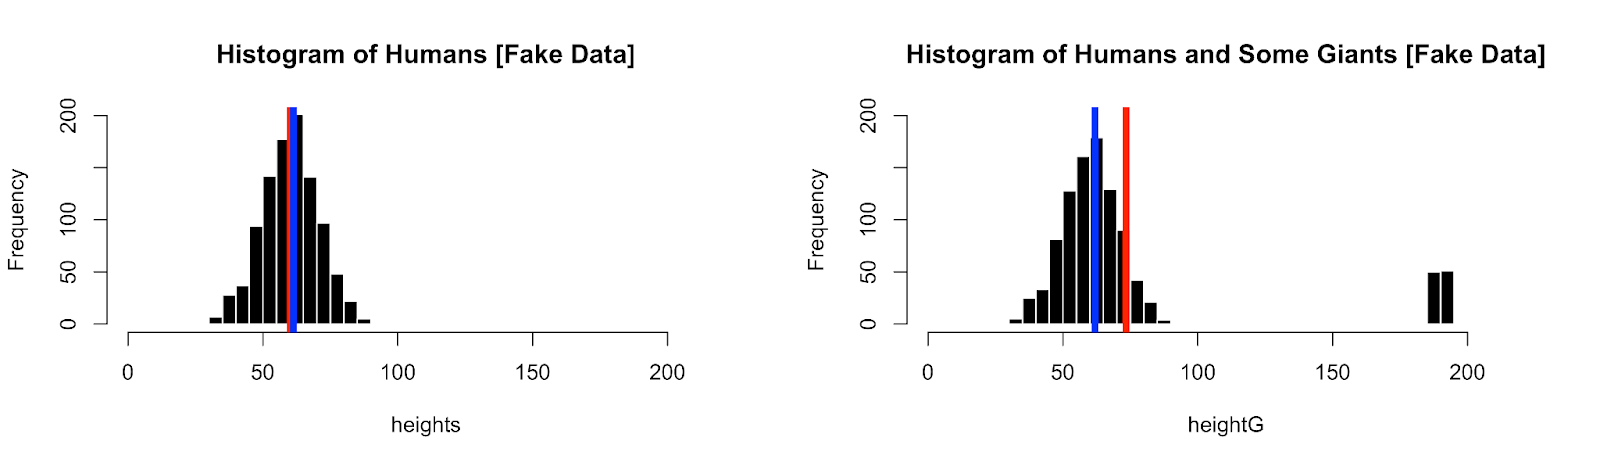
\includegraphics[keepaspectratio]{chapters/images/3_MedianvMean.png}}
\end{center}

\subsection{The Mode}\label{the-mode}

\subsubsection{The Definition}\label{the-definition-1}

The \textbf{mode} is the most common number in a set of numbers. If two
numbers are equally common in a distribution, then the distribution is
said to be bi-modal (and more than two most common numbers = multimodal)

So if your distribution was : 2, 3, 3, 5, 10, 14, 19, 20, 20, then the
mode would be\ldots{}\footnote{the mode would be 3 and 20, since these
  are the most frequent}

\subsubsection{Why It Matters}\label{why-it-matters-1}

The mode is rarely reported in research articles - I sometimes see it in
within-person studies, or in situations where researchers are measuring
psychophysiological measures (like heart rate or vagal tone) where the
peak of the distribution might indicate something important.

Conceptually, it can be interesting to note the presence of a mode, and
to think about why a bi-modal (or multi-modal) distribution occurs.~

For example, look at the following illustration : why might this bimodal
distribution occur?

\pandocbounded{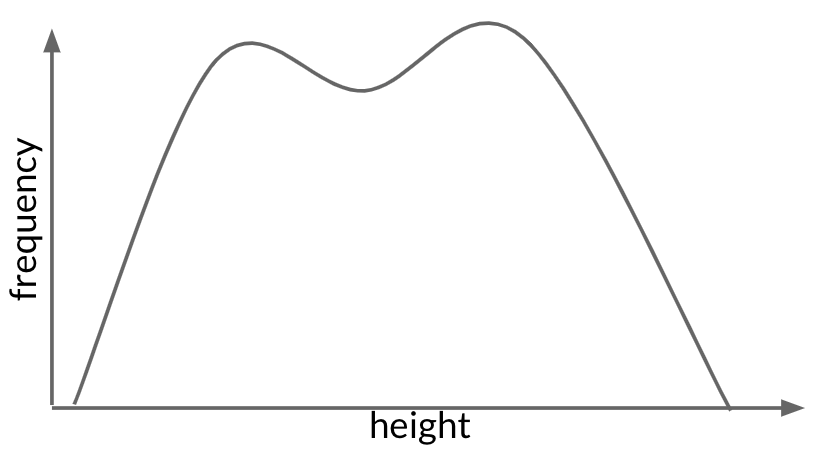
\includegraphics[keepaspectratio]{chapters/images/3_bimodalwhy.png}}

\begin{tcolorbox}[enhanced jigsaw, toptitle=1mm, toprule=.15mm, rightrule=.15mm, breakable, left=2mm, colbacktitle=quarto-callout-tip-color!10!white, colback=white, opacityback=0, coltitle=black, bottomtitle=1mm, opacitybacktitle=0.6, titlerule=0mm, leftrule=.75mm, arc=.35mm, bottomrule=.15mm, title=\textcolor{quarto-callout-tip-color}{\faLightbulb}\hspace{0.5em}{Reasons for this bimodal distribution.}, colframe=quarto-callout-tip-color-frame]

\begin{longtable}[]{@{}
  >{\raggedright\arraybackslash}p{(\linewidth - 2\tabcolsep) * \real{0.5212}}
  >{\raggedright\arraybackslash}p{(\linewidth - 2\tabcolsep) * \real{0.4788}}@{}}
\toprule\noalign{}
\endhead
\bottomrule\noalign{}
\endlastfoot
The more conventional answer is that this bimodal distribution
represents overlap between male and females in a dataset.

\pandocbounded{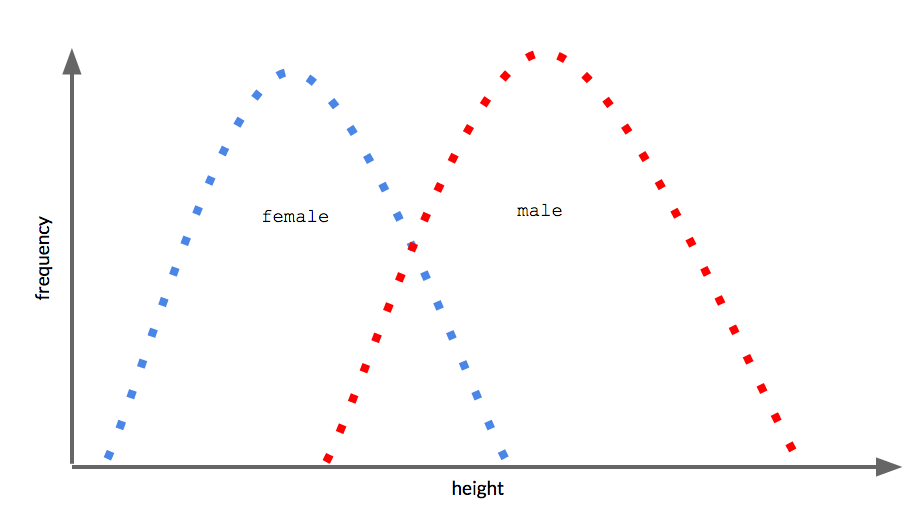
\includegraphics[keepaspectratio]{chapters/images/3_boringbimodal.png}}
& \begin{minipage}[t]{\linewidth}\raggedright
Another possibility is that this graph illustrates a python who has
swallowed an elephant.\footnotemark{}\\

\pandocbounded{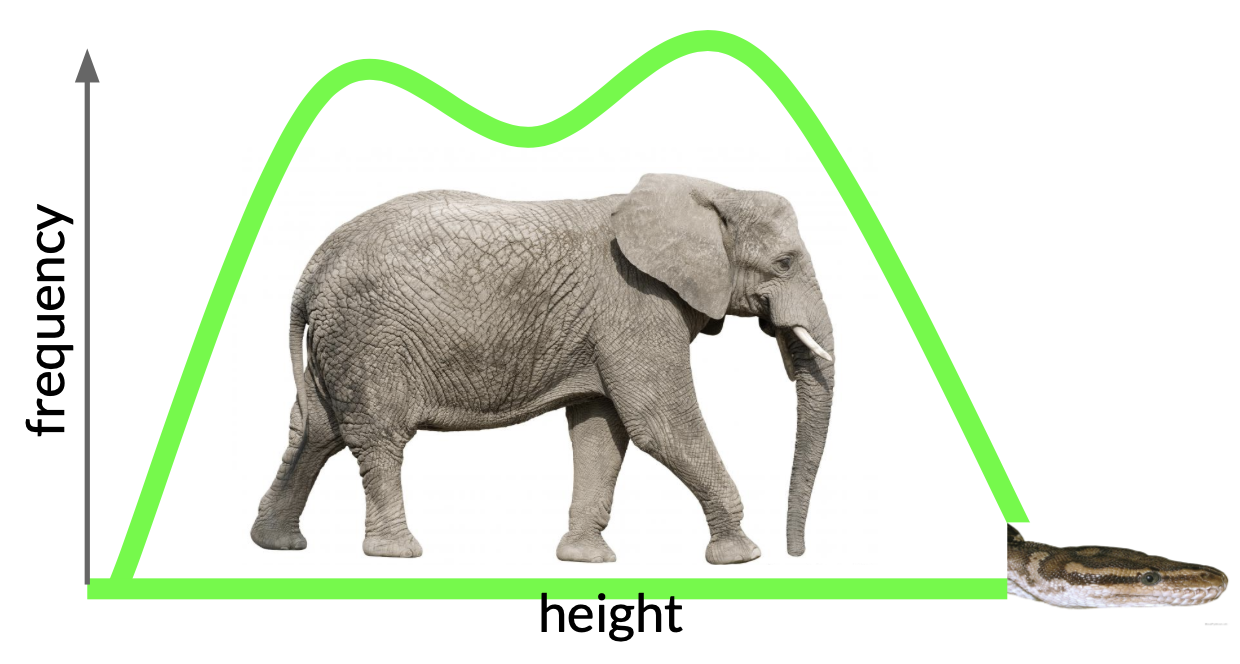
\includegraphics[keepaspectratio]{chapters/images/3_hateleephant.png}}\strut
\end{minipage} \\
\end{longtable}

\end{tcolorbox}

\footnotetext{see Antoine de Saint-Exupéry's (1943). The Little Prince.}

\section{Complexity}\label{complexity}

Complexity refers to the ways that data differ from each other - really
the focus of variation. And yet, as scientists, we are trying to
understand patterns in that variation, and so have developed a language
to talk about some of the systematic ways that individuals differ.

\subsection{Range.}\label{range.}

\subsubsection{Definition.}\label{definition.-1}

One way people differ is by the extreme ends; this is called \textbf{the
range}. Most people refer to the range as the lowest and highest value;
though sometimes the range is defined as the distance between the
highest and lowest value.

\subsubsection{Why It Matters.}\label{why-it-matters.-1}

The extreme low and high of your variable give you a sense about the
limits of variation. How to interpret these limits really depends on the
variable you are measuring; for a variable like reaction time in some
cognitive task, I would expect the low end to be zero (or something near
zero, but not negative) and the high end influenced by how long I would
expect the task to take (usually anywhere from less than a second for a
quick reaction to a few minutes.) If the high end of the range was
something like 30-minutes, I would think that something went wrong.

As a researcher (and teacher) I often use the range as a quick way to
ensure the data are correct - that is, to confirm that the lowest and
highest scores are possible values given the way the variable was
measured. For example, I check the range when looking at test scores to
make sure no students got a negative score or score above 100\% (both
impossible in my class.)

\subsection{Outliers.}\label{outliers.}

\subsubsection{The Definition}\label{the-definition-2}

Outliers are extreme values that are so different from the rest of the
data that you remove them from the dataset because you worry that they
might cause problems for your data. Outliers exist because of errors in
data entry (for example, the person who lists their age as 1009 instead
of 19) or because they represent individuals who are qualitatively
different from the rest of your data (for example, the participant who
is a billionaire and lists that as their income.\footnote{No shame
  billionaires! You are just very different from the rest of us. Let us
  know if I can hang out on your yacht? You belong to an understudied
  group and I have some research ideas. kthxbye.})

How extreme is too extreme? Some folks like to come up with rules for
making this decision based on the number of standard deviations away
from the mean or some other metric. I appreciate those efforts, but
personally believe it's better to judge outliers based on the
qualitative decisions above (and use past research as a guide). Whatever
you do, make sure to (1) justify your decisions, (2) report these
decisions in your code and analyses, and (3) make any decisions about
removing outliers as early as possible and before you start making
predictions.

\subsubsection{Why It Matters.}\label{why-it-matters.-2}

The presence of outliers in your data has the potential to influence
your results in ways that will bias your results. For example, if
someone wandered off in the middle of a cognitive task, their outliers
for reaction time might make you think people took way longer to
complete the task than people really needed to take. If I included
everyone who didn't take the exam (and got a zero) in taking the average
of the exam score, I might think that students did worse on the exam
than they really did, when I should have excluded these zeros to get a
better representation of how people did on the exam.

It's therefore super critical to a) identify any possible outliers in
the data, and b) remove them from data analysis, and c) be 100\%
transparent that you have removed data. You will learn to do this using
R in Part 4 below.

\subsection{Skew.}\label{skew.}

\subsubsection{Definition.}\label{definition.-2}

Skew describes asymmetry in the shape of the distribution. A graph that
is symmetrical has no skew.

\begin{center}
\pandocbounded{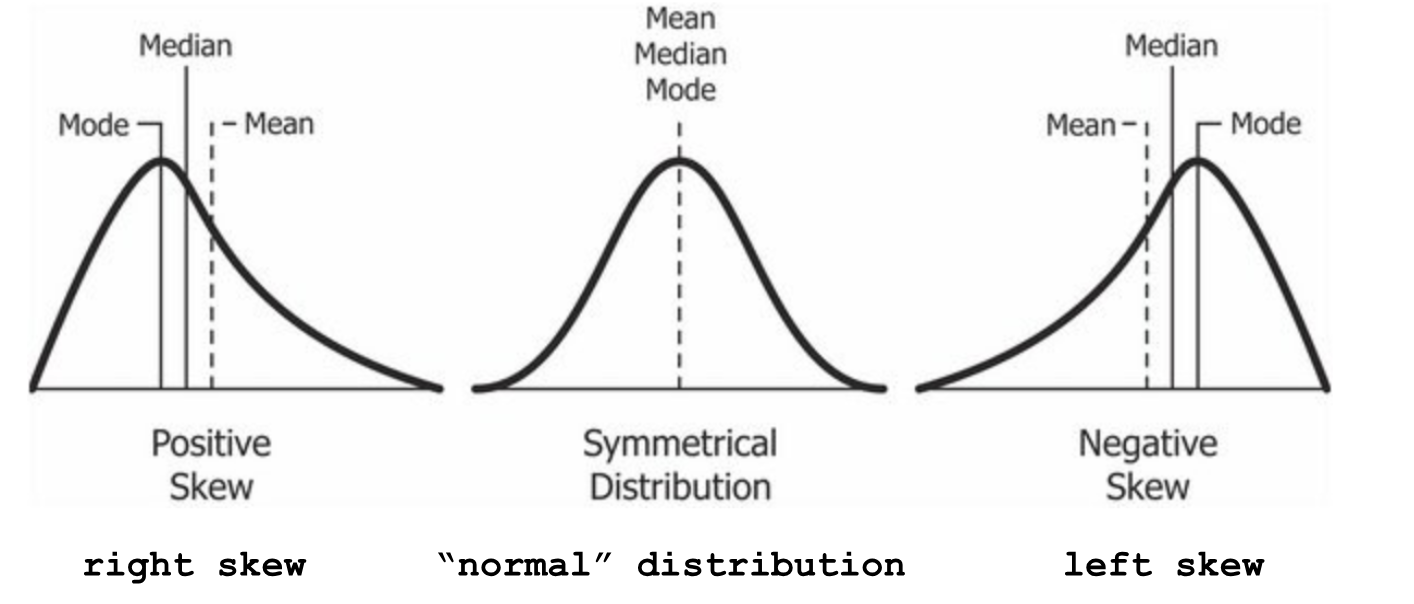
\includegraphics[keepaspectratio]{chapters/images/3_skewgraphs.png}}
\end{center}

It's easy to confuse the different types of skew, so I like to think of
skew as a type of pokemon (``pikaskew''), where the direction of
skewness is defined by its tail, since Pokemon (at least the ones I can
think of) have tails. This is my trick; feel free to use it (you are
welcome) or develop your own!~

\textbf{skew → pikachu →}

\includegraphics[width=1.0625in,height=\textheight,keepaspectratio]{chapters/images/3_pikaskew.png}\textbf{--\textgreater{}
tail}

\subsubsection{Why It Matters.}\label{why-it-matters.-3}

Skew can help us to think about why people

\begin{itemize}
\item
  \textbf{Negative Skew (also called ``Left Skew'')} is when the
  distribution ``tail'' sticks out on the negative (low) end of the
  measure. A negatively skewed distribution means that there's a greater
  probability of high scores than low scores, and can be explained by
  ceiling effects (a measure does not differentiate between high scorers
  - like an exam that almost everybody aces because you were all
  prepared.)
\item
  \textbf{Positive Skew (also called ``Right Skew'')} is when the
  distribution ``tail'' sticks out on the positive (high) end of the
  measure. A positively skewed distribution means that there's a greater
  probability of low scores than positive scores, and can be explained
  by floor effects (a measure does not differentiate between low
  scorers).
\item
  \textbf{No Skew (also called the ``Normal Distribution'')} is when the
  distribution is symmetrical.
\end{itemize}

\subsection{Kurtosis}\label{kurtosis}

Kurtosis describes the size of the tails, relative to the middle of the
distribution. I think of kurtosis as the pointiness of the distribution.
Mesokurtic is a distribution that looks ``normal'', leptokurtic is a
distribution that is skinny in the middle (with many individual scores
in the tail of the distribution), and platykurtic is a distribution wide
in the middle with few observations in the tails.

\begin{center}
\pandocbounded{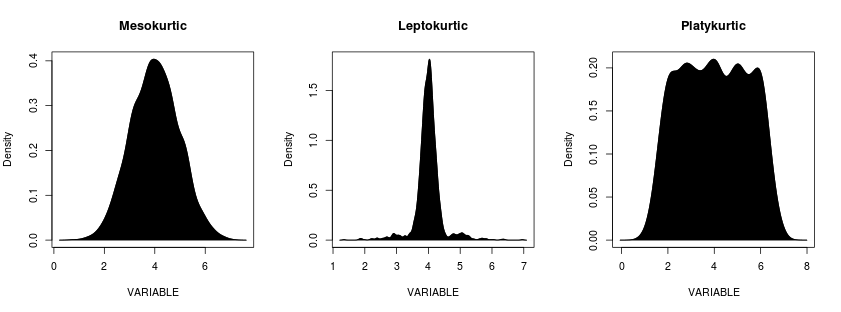
\includegraphics[keepaspectratio]{chapters/images/3_Kurtosis.png}}
\end{center}

Like skew, there are ways to quantify kurtosis, but we won't cover this
in the class. I almost never see kurtosis reported as a statistic in
journals.

\section{The Standard Deviation : A Mix of Centrality and
Complexity}\label{the-standard-deviation-a-mix-of-centrality-and-complexity}

\subsection{The Definition}\label{the-definition-3}

Standard Deviation (sd) is a way to quantify the `average' variation in
your dataset. More specifically, it is the average distance between all
individual data points in the distribution, and the mean of the
distribution. These distances (between an individual score and our
prediction) are called residuals.

The standard deviation is always positive, since it describes the
average distance of individual scores from the mean (residuals), and not
whether those residuals are above or below the mean. A standard
deviation of zero means there is no variation - all scores in the
distribution are the same. The larger the standard deviation, the more
variation there is in the data. There's no limit to how large the
standard deviation might be.

Understanding what the standard deviation is, and how it's calculated,
is a critical skill. In the videos below I walk through how to calculate
standard deviation by ``hand''. You will never actually use this
approach in real-life, but I find it very helpful to fully understand
what a standard deviation is, and how (and why) we use residual scores
in statistics. With the chickenweights dataset, of course.

\subsubsection{Video : The Mean as
Prediction}\label{video-the-mean-as-prediction}

With no other knowledge about an individual, the mean is our best
prediction about what an individual is like.

\url{https://youtu.be/sK6_vcs23I0}

\subsubsection{Video : Residuals as
Error}\label{video-residuals-as-error}

\textbf{Residuals} refer to the fact that the mean is not a perfect
prediction for every person; people will differ from our predictions.
These differences between each individual's actual score and our
predicted value (in this case, the mean) are called residuals. The
residuals will always be actual score minus prediction - I remember this
because as researchers we care about actual people first.

\url{https://youtu.be/AGl7jo3WRJY}

\subsubsection{Video : The Sum of (Squared) Residual
Errors}\label{video-the-sum-of-squared-residual-errors}

\textbf{The sum of squared errors (SS)} is a way to quantify the total
residuals when using the mean to make predictions. As you'll see in the
video, we must first square the residual differences in order to remove
the direction (since we care about the total error, not whether the
individual was above or below our prediction.). And then we sum these
squared differences to quantify the total (squared error).

\url{https://youtu.be/hN5opflzXIA}

\subsubsection{Video : The (Unsquared) Average of These Squared
Residuals = Standard
Deviation}\label{video-the-unsquared-average-of-these-squared-residuals-standard-deviation}

\textbf{The standard deviation} is the squared root of these averaged
squared differences. Or, in less technical terms, the standard deviation
is the average of how much people differ from the mean - a measure of
the average variation.

\url{https://youtu.be/4SQUK8GXwrI}

\subsection{Why This Matters}\label{why-this-matters}

Great question! The standard deviation does two things :

\begin{enumerate}
\def\labelenumi{\arabic{enumi}.}
\tightlist
\item
  The standard deviation quantifies how much the ``average'' person
  differs from the average of the individuals in a group. This is a
  great statistic to have, since it quantifies how much individuals
  differ from each other on average (between-person variation)
\item
  The standard deviation serves as a baseline for our predictions. The
  mean is a GREAT starting place for our predictions, but soon we will
  want to make more sophisticated predictions. We will do this with our
  good friend \emph{the linear model}, and will know whether we can
  improve our predictions by decreasing the amount of residual error.
\end{enumerate}

\chapter{Part 2 : Describing Data in
R}\label{part-2-describing-data-in-r}

\section{Video : Describing Happiness (World Happiness
Report)}\label{video-describing-happiness-world-happiness-report}

In this video, I walk through loading the World Happiness Report (in our
Chapter Dataset folder on the course page), and describing and graphing
the happiness variable.

\url{https://youtu.be/Te1ChWgiATU}

\section{Video : Standard Deviation of Happiness (World Happiness
Report)}\label{video-standard-deviation-of-happiness-world-happiness-report}

In this video, I review how to calculate the standard deviation, and
what this statistic tells you about the variable happiness.

\url{https://youtu.be/Pm8Z2z6QWMs}

\section{R Code : Descriptive
Statistics}\label{r-code-descriptive-statistics}

Below is a list of code we'll use to calculate descriptive statistics in
R.

\begin{longtable}[]{@{}
  >{\raggedright\arraybackslash}p{(\linewidth - 2\tabcolsep) * \real{0.1319}}
  >{\raggedright\arraybackslash}p{(\linewidth - 2\tabcolsep) * \real{0.8681}}@{}}
\toprule\noalign{}
\endhead
\bottomrule\noalign{}
\endlastfoot
\textbf{R Command} & \textbf{What It Does} \\
\texttt{summary(dat)} & Reports descriptive statistics for all variables
in the dataset. \\
\texttt{summary(dat\$variable)} & Reports descriptive statistics for a
continuous variable.

Reports frequency for a categorical variable. \\
\texttt{mean(dat\$variable,\ na.rm\ =\ T)} & Reports the mean (average)
of a variable; you must include the na.rm = T argument if there is
missing data (otherwise R will return NA as the result). \\
\texttt{median(dat\$variable,\ na.rm\ =\ T)} & Reports the median
(middle point) of a variable. \\
\texttt{range(dat\$variable,\ na.rm\ =\ T)} & Reports the lower limit
and upper limit of the variable. \\
\texttt{sd(dat\$variable,\ na.rm\ =\ T)} & Reports the standard
deviation of the variable. \\
\texttt{hist(dat\$variable)}

\texttt{abline(v\ =mean(dat\$variable))} & Draws a line on a plot or
histogram at specified values (e.g., this draws a vertical line at the
mean of dat\$variable. You can replace v with h to draw a horizontal
line. We will use abline() later in the semester in a different way. \\
\texttt{par(mfrow\ =\ c(i,\ j))} & Splits your graphics window into i
rows and j columns (replace i and j with numbers) \\
\end{longtable}

\section{\texorpdfstring{\href{https://docs.google.com/forms/d/e/1FAIpQLScJ2ZvwLv2D4SYXFN2NL-7M8-B3Acq9BXsS1HwJSPf-LnGx4w/viewform?usp=sf_link}{Practice
Quiz with R} : Practice Quiz 3 (Describing
Variables)}{Practice Quiz with R : Practice Quiz 3 (Describing Variables)}}\label{practice-quiz-with-r-practice-quiz-3-describing-variables}

\textbf{Instructions}

Use R and the twitter\_emotion\_data.csv to answer the following
questions in the check-in above.

\begin{itemize}
\item
  Here's a
  \href{https://www.dropbox.com/scl/fi/zye2fojtmol8wdmd1gfb7/twitter_emotion_data.csv?rlkey=t728np5edvmw3wjoorj2hddwu&dl=0}{\textbf{link
  to the dataset}} (load this into R) and a
  \href{https://www.dropbox.com/scl/fi/0q0meai7hawk4oexw948c/CODEBOOK-_-Twitter-Emotion-Dataset.pdf?rlkey=yz6aiqtow6k4ey16k8qd0y4yz&dl=0}{link
  to the Codebook} (that describes the dataset)
\item
  \href{https://youtu.be/L3kQXfp2jNg}{\textbf{Link to a video
  key}}\textbf{;} but good to try this on your own!
\end{itemize}

\textbf{Questions}

\begin{enumerate}
\def\labelenumi{\arabic{enumi}.}
\item
  Load the data and check to make sure the data loaded correctly. How
  many individuals (tweets; in this dataset, each row = one tweet) are
  in the dataset?
\item
  Graph the variable retweet\_count. How would you describe the shape of
  this variable?
\item
  What do you learn about the variable retweet\_count from this graph?
\item
  What is the mean of the variable retweet\_count?
\item
  What is the median of the variable retweet\_count?
\item
  What is the standard deviation of the variable retweet\_count? {[}note
  : you do not need to do this by hand{]}?
\item
  What is the lowest value (range) of the variable retweet\_count?
\item
  What is the highest value (range) of the variable retweet\_count?
\item
  Now, work with the categorical variable Orientation. How many Liberal
  (tweets) are in the dataset?
\item
  How many Conservative (tweets) are in the dataset?
\end{enumerate}

\section{Video : Removing Outliers}\label{video-removing-outliers}

The video below describes how to remove outliers, using a datset built
into R.

\url{https://youtu.be/Hi0C8M5398Q}

We will practice removing outliers in lecture! It will get easier.

\chapter{Part 3. Research for Fun and
Profit}\label{part-3.-research-for-fun-and-profit}

Researchers share their knowledge with others in \textbf{scientific
articles}. These are written by researchers for other researchers, tend
to be very detailed and technical, and are a researcher's golden ticket
to getting a job, research grant, invited talk or book deal, podcast
invitation, etc. So there's a lot of pressure to publish research among
academics.

\section{The Publication Process}\label{the-publication-process}

Researchers spread their scientific knowledge by publishing research
papers. You can read more about how researchers publish research HERE.
However, the TLDR is something like this :

\begin{enumerate}
\def\labelenumi{\arabic{enumi}.}
\item
  \textbf{Researcher has an idea!} They assemble a team of others
  interested in the idea, and do a literature review in order to gain
  background knowledge on the topic.
\item
  \textbf{Researcher designs a study, collects data, analyzes the data,
  and writes up the data as a report.} All the steps of the scientific
  method. This is what you will do for the final project!
\item
  \textbf{Researcher submits the report to a scientific journal.} A
  journal is a collection of articles that are usually united by some
  common theme. In general, the shorter the name of the journal, the
  more prestigious\footnote{Prestige is a very subjective concept in
    science. However, scientists have found many ways to quantify it, as
    described in the sections below!}. For example, the ``Journal of
  Research in Personality'' is considered less prestigious than the
  ``Journal of Personality and Social Psychology'', which is less
  prestigious than the journal called ``Psychological Science'', which
  is considered less prestigious than the journal called ``Science''.~
\item
  \textbf{An editor decides whether to review or reject the article.}
  Editors make an initial decision - based on a summary of the study and
  a letter that the author writes to the editor - whether the research
  article might be a good fit for the journal. If so, they pass it along
  to the next step. If not, they send a ``Thanks, but\ldots.'' rejection
  letter.
\item
  \textbf{The editor sends the article to peer-reviewers.} Peer
  reviewers are other researchers who have some related research
  interests or skills in the topic of the paper. They will look over the
  article. The editor may know these people, or they get asked by
  another peer-reviewer who didn't want to do it but nominated someone
  else to step into the role. Peer-reviewers work on a completely
  voluntary basis - it's seen as required service, and there's a bit of
  professional reputation to maintain in doing this work. Yes, there are
  problems with unpaid labor in academia. We can chat about that if
  you'd like; ask questions / raise it as an issue on Discord.
\item
  \textbf{The editor makes a decision on the paper based on the feedback
  from the peer-reviewers.} The editor summarizes the feedback, and
  either accepts the paper, accepts as long as the person makes
  necessary revisions, asks the researcher to ``Revise and Resubmit''
  (this is called an R\&R - probably the most common outcome, and does
  not guarantee that the paper will be accepted if the revisions are
  made, but will get sent out to peer-reviewers again), or rejects the
  paper. In any case, the author will see the comments made by the
  peer-reviewers and the editor.
\item
  \textbf{The (accepted) paper goes to a proofreader and is published.}
  Hooray! This process probably takes anywhere from 6 months (insanely
  fast) to 2 years (or more, depending on the number of revisions that
  are required).
\end{enumerate}

\section{Publish! Or Perish\ldots?}\label{publish-or-perish}

Ask any grad student or professor - the publication process is
stressful, unpredictable, slow, and threatening. Grad students are
required to publish papers in order to have a chance at an academic job
as a researcher (and even extremely productive and thoughtful graduate
students are not guaranteed an academic job), professors are required to
publish papers in order to get a chance of getting tenure (and even
extremely productive and thoughtful researchers are not guaranteed
tenure).

This creates incredible pressure on researchers to get results; pressure
that often can interfere with people's ability to do GOOD science. We'll
talk about this more throughout the semester; bring questions to class /
Discord!

\section{Types of Research Articles}\label{types-of-research-articles}

We'll learn how to read and dissect scientific articles this semester,
but first it will be important to learn how to identify There are a few
different types of articles that researchers write :

\begin{enumerate}
\def\labelenumi{\arabic{enumi}.}
\item
  \textbf{Original Reports :} An original report is where the
  researcher(s) write about the results of a novel study they did to
  test some theory. This means the researchers did something ``new'' -
  usually they collected and analyzed new data to test a theory, or
  analyzed existing data in a new way. Here's an example of an original
  report on the topic of emotion regulation.
\item
  \textbf{Replication :} A replication is a type of study where a
  researcher repeats the steps they (or another) researcher did, and
  sees if they get the same result. As we discussed, psychology (and
  many other fields) is in a \textbf{replication crisis.} This type of
  article was not very common before the 2010s, but is more common now.
  Still, faculty tend to be biased toward producing original reports - a
  school like Berkeley or Stanford would not hire a researcher just for
  doing replications. Here's an example of a replication on the topic of
  emotion regulation. Note this is not really a direct replication,
  since they replicated in a different population.
\item
  \textbf{Meta-Analyses :} A meta-analysis is where researchers take
  other people's data, collect it, and analyze it in order to see broad
  trends across an entire field. For example, a meta-analysis might take
  all the research on whether there's a relationship between playing
  violent video games and violent behavior, and analyze this existing
  research in terms of common themes, such as the type of video games
  the researchers studied, the measures of violence, and the results.
  Meta-Analyses can be a great way to look at a broad trend, but they
  rely on the assumption that the individual studies they summarize are,
  in fact, valid themselves. That is, if there are systematic biases in
  the way researchers study a topic, the Meta Analysis won't solve or
  even identify those problems. Here's an example of a meta-analysis
  done on the topic of emotion regulation.
\item
  \textbf{Review Article :} Review articles summarize existing research
  without doing any additional data analysis (in contrast to a
  Meta-Analysis, in which there is data analysis of past research). This
  is the closest thing to a paper you might write in an English class -
  the authors take past research, summarize it in terms of common
  themes, and maybe highlight limitations, or new directions the field
  might take. Review articles are a great way to get a broad overview of
  a topic, since they summarize and organize past research, and will
  often highlight next steps that researchers should take. Here's an
  example of a review article done on the topic of emotion regulation.
\end{enumerate}

\section{The Peer Review Process}\label{the-peer-review-process}

In order to publish their results, researchers have their peers review
their work, and provide comments or suggestions. The peer-review process
ideally serves two purposes :~

\begin{enumerate}
\def\labelenumi{\arabic{enumi}.}
\item
  \textbf{Peer Reviewers Help Improve the Research.} The peers doing the
  reviewing are supposed to have expertise in the topic of the paper.
  This allows them to suggest ways to improve the paper. These
  suggestions can run from the simple (such as recommending other
  researchers to reference in the introduction or additional analyses to
  run) to very involved (suggestions for additional studies to run,
  different methods to use, or different people to study).
\item
  \textbf{Peer Reviewers Provide a Vote of Confidence in the Ideas and
  Analyses of the Paper.} The editor of a journal will look to the peer
  reviewers for evidence that the research is ``high quality'' and / or
  novel enough to be published. There's a fair amount of bias here -
  some reviewers think the research is good but not considered a ``good
  fit'' for the journal. But the ``peer-reviewed'' label of a journal
  gives at least one layer of confidence that some other people like
  this research.
\end{enumerate}

One important aspect of the peer-review process is that the
peer-reviewers are anonymous to the author, and sometimes the author is
anonymous to the peer-reviewers. Ideally, this helps prevent previous
beliefs bias (since some researchers may have positive or negative
impressions of each other) and social influence bias (since a famous
researcher at a fancy school may have their research more trusted than
someone with less prestige to their name or institution). However,
psychological fields are often small enough that people tend to know
who's doing what research, and there are other cues that can tip
peer-reviewers off about who the author of a study is (for example, the
author of a study will likely reference their own work, since their new
study builds off their old study.)

\begin{tcolorbox}[enhanced jigsaw, toptitle=1mm, toprule=.15mm, rightrule=.15mm, breakable, left=2mm, colbacktitle=quarto-callout-warning-color!10!white, colback=white, opacityback=0, coltitle=black, bottomtitle=1mm, opacitybacktitle=0.6, titlerule=0mm, leftrule=.75mm, arc=.35mm, bottomrule=.15mm, title=\textcolor{quarto-callout-warning-color}{\faExclamationTriangle}\hspace{0.5em}{Academic Publishers are Predatory Capitalists.}, colframe=quarto-callout-warning-color-frame]

\begin{longtable}[]{@{}
  >{\raggedright\arraybackslash}p{(\linewidth - 2\tabcolsep) * \real{0.0349}}
  >{\raggedright\arraybackslash}p{(\linewidth - 2\tabcolsep) * \real{0.9651}}@{}}
\toprule\noalign{}
\endhead
\bottomrule\noalign{}
\endlastfoot
\pandocbounded{
\includegraphics[keepaspectratio]{chapters/images/angry_mickey.png}}
& You know how the music business can hurt artists and interrupt the
free flow of groovy music??? Well, academic publishers are no different,
and can make profits in the billions of dollars. They do this by
charging exorbitant fees for accessing peer-reviewed articles, and not
paying the researchers who publish papers any money. That's right;
researchers get a 0\% commission of any sales of their academic
articles. It is a horrible and corrupt system that deserves to die.

But you don't have to take my word for it! You can read more about the
\href{https://bigthink.com/surprising-science/open-access-academic-publishers/}{\textbf{problem
with publishers and a (controversial) solution - sci-hub}} - here.
Here's an
\href{https://www.theguardian.com/science/2017/jun/27/profitable-business-scientific-publishing-bad-for-science}{\textbf{{[}OPTIONAL{]}
longer article}}that goes into the history of academic publishing, and
why it's so corrupt.
\href{https://www.youtube.com/watch?v=usDdBOGdEV0}{Here's a video}that
covers some of the same info.
\href{https://www.theverge.com/2018/2/8/16985666/alexandra-elbakyan-sci-hub-open-access-science-papers-lawsuit}{\textbf{Here's
an even longer article}} that goes into sci-hub and ``scientific
communism''. Feel free to skim or skip all of this! But lemme know if
you read / found something you thought was interesting :) \\
\end{longtable}

\end{tcolorbox}

\section{Finding Research Articles}\label{finding-research-articles}

Next week we will find research articles related to YOUR research
interests. I like to use Google Scholar for this - I find the search
features powerful and Google will comb the internet for free versions of
research articles (so I don't have to be on campus or have proxy access
to UC Berkeley's library or ``steal'' articles from publishers using
sci-hub).

For example, searching for one of my dissertation chapters shows
\href{https://scholar.google.com/scholar?hl=en&as_sdt=0\%2C5&q=situational+suppression&btnG=}{this
page}.

\pandocbounded{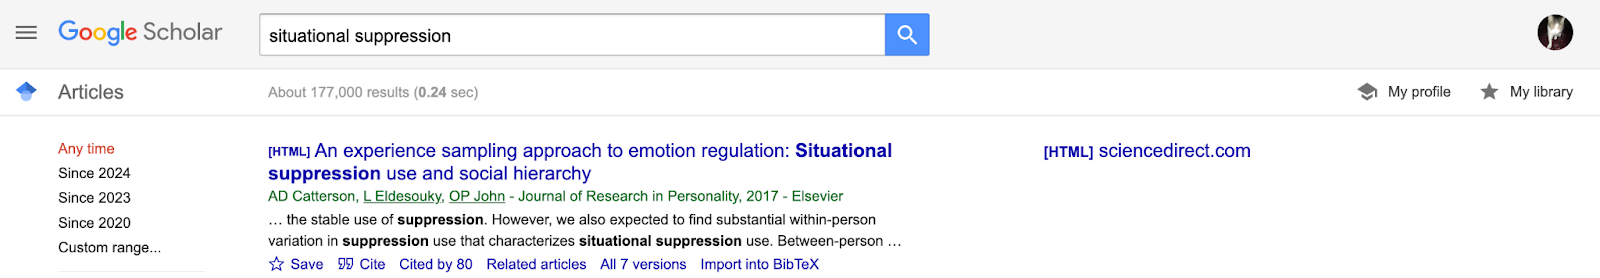
\includegraphics[keepaspectratio]{chapters/images/5_DissChapterGoogle.png}}\\

\subsection{\texorpdfstring{\textbf{How to Find
Articles}}{How to Find Articles}}\label{how-to-find-articles}

Some tips for finding an article related to your topic :~

\begin{enumerate}
\def\labelenumi{\arabic{enumi}.}
\item
  \textbf{Use the right ``jargon''.} As part of the operationalization
  process, scientists use specialized terms. What you might call
  ``holding it in'' researchers call ``expressive suppression''; a
  ``jerk'' would be someone ``low in agreeableness''; that feeling of
  ``being hella stressed before an exam but also low key stepping up
  because of that stress'' is the ``psychophysiological distinction
  between challenge and threat''. As you search for research related to
  your topic, take note of how researchers are describing related
  phenomena, and adjust your terms as needed. This is part of building
  your schema for the topic.
\item
  \textbf{Look at past research on the topic.} If you've found a
  relevant article on your topic, it's likely that the article has
  referenced other research that is also relevant. Read or scan through
  the introduction (or the references section) and see if there's
  something that looks related to your interests.
\item
  \textbf{Look at future research on the topic.} If you found a relevant
  article on your topic, it's likely that other researchers have also
  read that article, and used it in their future research. Google
  Scholar has a ``Cited By'' button
  {[}\includegraphics[width=0.41667in,height=0.13542in]{index_files/mediabag/AD_4nXdWGVqSlFveQI-X.png}{]}that
  you can use in order to see more recent articles that have referenced
  the article you found. This is a particularly useful way to find more
  recent research if you found a ``classic'' in the field, or check for
  replications or controversies.
\item
  \textbf{Old Research is Okay! But look for new research too.} Many
  students wonder if an ``old'' study is still relevant. Some papers are
  ``classics'' in the field, and great to read. But it's likely that our
  field's understanding of self-esteem has changed from 1970. If you are
  hoping to build your schema on a topic, finding a review article from
  the last 10 years (or 5; or 2!) would be a good place to start.
\end{enumerate}

\subsection{How to Evaluate an
Article}\label{how-to-evaluate-an-article}

It can often be overwhelming for students to sift through the masses of
research on a topic and know what's most important and relevant.~

Reading the article and using your critical thinking skills /
psychological training is the best approach. To do this, it is
recommended to \textbf{go to Graduate School,} where you canspend
multiple years reading as much as you want on a beautiful college
campus, taking classes where you can deeply engage with the research and
ideas, immerse yourself in meaningful intellectual conversations had by
other graduate students and kindly professors - the gleam of knowledge
and excitement of supporting the next generation of researcher in their
eye. Oh, that is not interesting to you / grad schools are flooded with
applications / you can't get an office hour appointment with your
professor who actually / you don't have the privilege of spending 5-8
years getting paid near-poverty wages to be a poor scholar?~

Well, below are a few other ideas to make superficial , all depending on
our good friend social influence bias :

\begin{enumerate}
\def\labelenumi{\arabic{enumi}.}
\item
  \textbf{The Citation Count.} Google scholar allows you to see how many
  other research articles have referenced the article that you found.
  While this can be a nice way to see how influential a paper is, a
  paper could be referenced a lot for reasons other than its validity,
  and maybe no one has read the most amazing paper in the world.
\item
  \textbf{The Impact Factor of the Journal.} Journals have different
  ``prestige factors'', and the impact factor is one way to quantify
  this prestige. Impact factor is usually defined as the number of times
  the average article in a journal has been referenced by other
  researchers in a year. So an impact factor of 2 means that each
  article in that journal is referenced by two other articles in a year.
  The impact factor is something you have to look up - journals usually
  track this. I wouldn't spend too much time worrying about it, but it's
  a quick way to get a very superficial sense of the journal's
  reputation. For example, let's see how the impact factor relates to
  our rule of ``broader journal name = more prestige''.
\end{enumerate}

\begin{longtable}[]{@{}
  >{\raggedright\arraybackslash}p{(\linewidth - 2\tabcolsep) * \real{0.5000}}
  >{\raggedright\arraybackslash}p{(\linewidth - 2\tabcolsep) * \real{0.5000}}@{}}
\toprule\noalign{}
\endhead
\bottomrule\noalign{}
\endlastfoot
\textbf{Journal} & \textbf{Impact Factor According to Google in 2024} \\
Journal of Research in Personality & 2.6 \\
Journal of Personality and Social Psychology & 6.4 \\
Psychological Science & 10.1 {[}couldn't find a recent stat on this
tho{]} \\
Science & 44.7 {[}this escalated quickly{]} \\
\end{longtable}

\begin{enumerate}
\def\labelenumi{\arabic{enumi}.}
\setcounter{enumi}{2}
\tightlist
\item
  \textbf{The Researcher and Institution.} Another way to evaluate an
  article is by evaluating the author. Does it look like this research
  has produced other cool research, or do you find their work boring and
  problematic for some reason? Is this researcher well known and
  respected in the field? Do they seem to have a happy photo with all
  their graduate students on their lab website, or is their lab website
  10 years old and just has one sad looking graduate student asking for
  help with their eyes? Has the researcher continued to produce
  interesting, reliable research? Or were they the subject of a
  replication scandal?
\end{enumerate}

\subsection{Video Examples : Using Google Scholar to Find
Research}\label{video-examples-using-google-scholar-to-find-research}

\subsubsection{Using Google Scholar}\label{using-google-scholar}

\url{https://youtu.be/j4dx9Cw_SuU}

\begin{itemize}
\tightlist
\item
  How to find articles, use the right jargon, and do some very
  superficial evaluations of the article's quality.
\end{itemize}

\subsubsection{Exporting APA Citations}\label{exporting-apa-citations}

\url{https://youtu.be/HWd4z4a67uE}

\begin{itemize}
\tightlist
\item
  The ``\,'' button on Google Scholar makes life so much easier!! No
  more memorizing APA format!! Hooray!!!
\end{itemize}

\chapter{TLDR.}\label{tldr.}

We learned how to describe variables in terms of consistency (e.g.,
mean, median) and complexity (e.g., range, standard deviation). We
focused on how to define the standard deviation, and then looked at how
to do this in R.

Next week in lecture, we will continue to learn to use R, statistics,
and our human brains to describe and understand how people differ.

\chapter{Measures}\label{measures}

This week, you'll learn about how (and why) a \textbf{likert scale} can
be used to define continuous variation, and how to create a likert scale
in R.

\chapter{Part 1 : Likert Scales}\label{part-1-likert-scales}

\section{Definition \& Theory}\label{definition-theory}

A likert scale is a common survey method psychologists use to measure
\href{https://docs.google.com/document/d/18nv4NsyRkjP3ClgreidOOWyxS3VdSQPpT2kRwfTHvm0/edit\#bookmark=id.hco904ai8j6f}{continuous
variation}. Likert scales can be used for self-report surveys (where an
individual answers questions about themselves), or given to observers
(where an individual answers questions about another person - either
someone they know, or someone they are actively observing).~For example,
to the right is an example likert scale - the Rosenberg Self-Esteem
Scale\footnote{Rosenberg, M. (1965). Rosenberg Self-Esteem Scale (RSES)
  {[}Database record{]}. APA PsycTests. Here's a link to
  \href{https://www.wwnorton.com/college/psych/psychsci/media/rosenberg.htm}{take
  the survey} and get feedback.

  \hfill\break
}. Here's a link to
\href{https://www.wwnorton.com/college/psych/psychsci/media/rosenberg.htm}{take
the survey} and get feedback.

\marginnote{\begin{footnotesize}

\pandocbounded{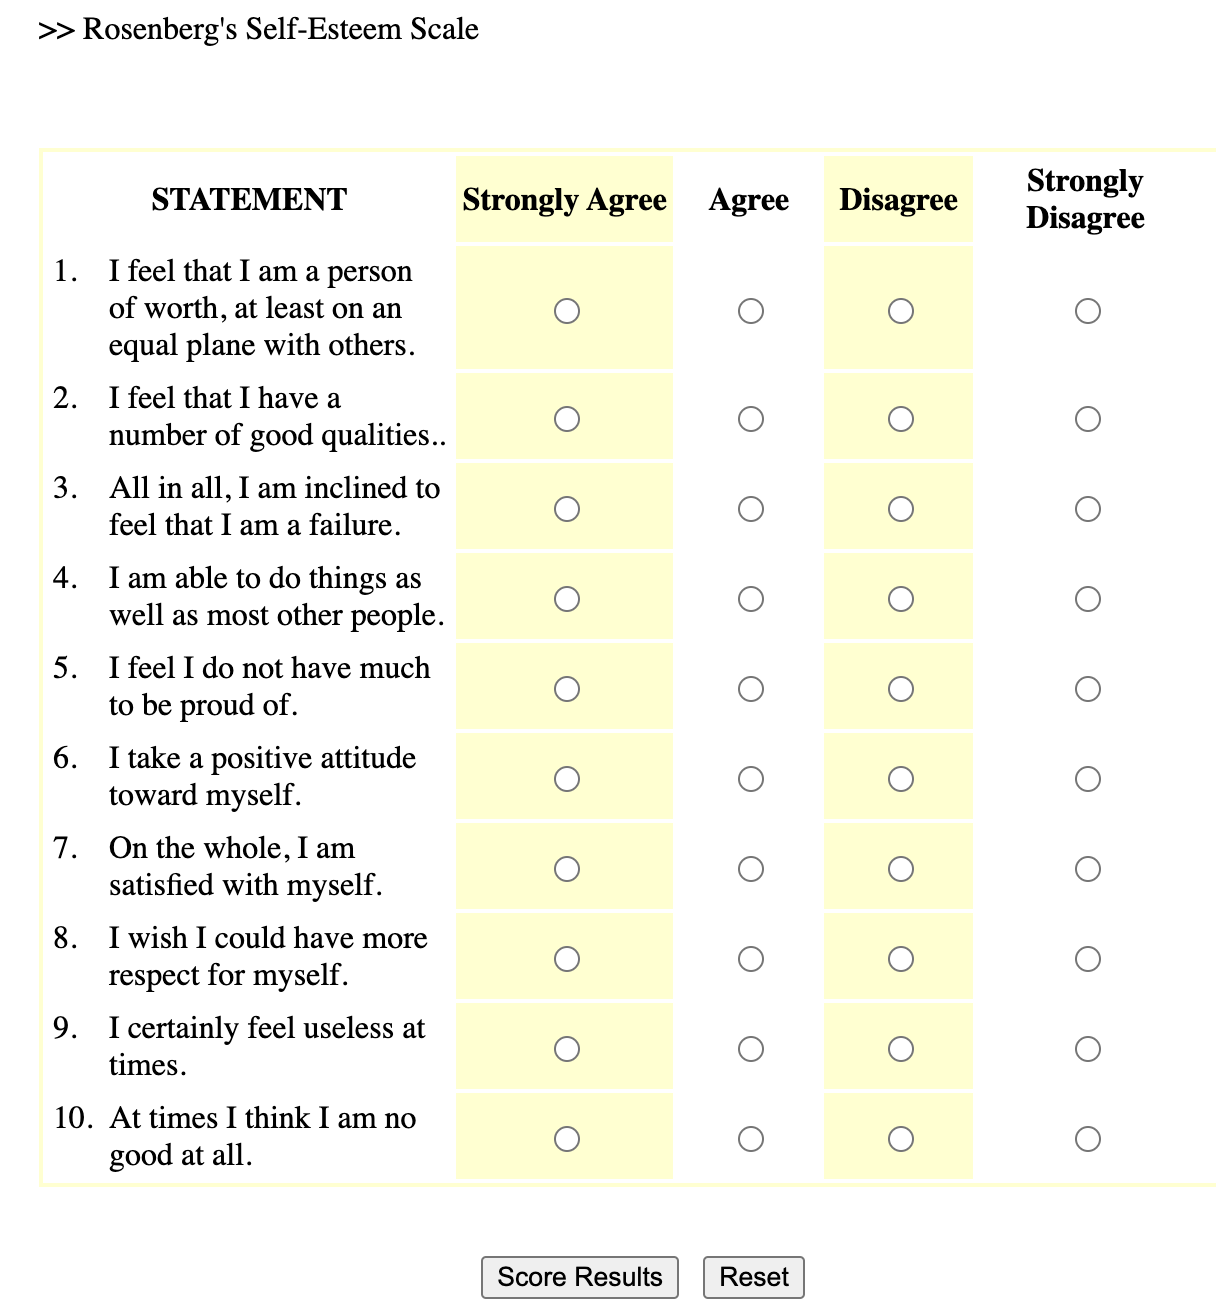
\includegraphics[keepaspectratio]{chapters/images/4_SWLS.png}}

\end{footnotesize}}

Below are some common terms we will use when describing likert scale.
(There's a video that goes over these terms with another example below
too.)

\begin{longtable}[]{@{}
  >{\raggedright\arraybackslash}p{(\linewidth - 4\tabcolsep) * \real{0.0389}}
  >{\raggedright\arraybackslash}p{(\linewidth - 4\tabcolsep) * \real{0.5500}}
  >{\raggedright\arraybackslash}p{(\linewidth - 4\tabcolsep) * \real{0.4097}}@{}}
\toprule\noalign{}
\endhead
\bottomrule\noalign{}
\endlastfoot
\textbf{Term} & \textbf{Definition} & \textbf{Usage / Example} \\
\textbf{Scale} & The variable that you want to measure as a continuous
variable. & Self-esteem is often measured with the Rosenberg Self-Esteem
Scale (1965) \\
\textbf{Item(s)} & The specific question(s) in the scale. Each item
measures some aspect of the variable the researcher is interested in. &
The Rosenberg Self-Esteem Scale (RSE; 1965) is a ten item scale, which
means it has ten questions about self-esteem. \\
\textbf{Response Scale} & How people answer the scale items. People give
a number rating on a fixed range of options with labels. Many 5-point
scales include the following labels (1 = Strongly Disagree; 2 =
Disagree; 3 = Neutral; 4 = Agree; 5 = Strongly Agree.) & The RSE was
originally written to use a 4-point rating scale from 0 (Strongly
Disagree) to 3 (Strongly Agree). When Professor includes the RSE in his
studies, he might change the response scale to go from 0-4 to so it has
an odd-number of answers to allow people to say they are ``neutral''. \\
\textbf{Positively-}

\textbf{Keyed Item} & An item that measures the high end of the scale,
where answering ``yes'' to the question means you are high on this
variable. & ``On the whole, I am satisfied with my life'' is a
positively-keyed item, because answering 4 (Strongly Agree) means the
person says they are high in self-esteem. \\
\textbf{Negatively-Keyed Item} & An item that measures the low end of
the scale, where answering ``yes'' to the question means you are low on
the variable. & ``I certainly feel useless at times'' is a
negatively-keyed item, because answering 4 (Strongly Agree) means the
person says they are low in self-esteem. \\
\textbf{Reverse Scoring} & How researchers ``flip'' the negatively-keyed
items to be positively-keyed. To calculate how to reverse-score an item,
you can add the lower and upper limit of the full range. So to
reverse-score a response scale that goes from 0 to 4 = 0 + 4 = subtract
the negatively keyed items from 4. A response scale that goes from 1 to
15 = 1 + 15 = subtract the negatively keyed items from 16. And so on.

This is confusing. We will practice in lecture some more, okay? & To
reverse score the negatively-keyed item, you would subtract the person's
4 from 4 (since the scale range is 0 to 4, so 0+4 = 4). A response of 4
(Strongly Agree) to the question I certainly feel useless at times means
that for this question, the person's self-esteem would be rated as a 0.

POP QUIZ : a survey has a response scale that goes from 1-7. What number
would you subtract from in order to reverse score a negatively-keyed
item?\footnote{You would subtract from 8, since 1+7 = 8. So a 7 for a
  negatively-keyed item on the 1-7 scale would be turned into a 1, since
  8-7 = 1} \\
\end{longtable}

\textbf{Advantages of Likert Scales}

\begin{enumerate}
\def\labelenumi{\arabic{enumi}.}
\item
  They are easy to administer as a self-report or observational survey,
  and provide structured data.
\item
  \textbf{The principle of aggregation} describes a phenomenon where
  combining multiple items into one scale will provide a more reliable
  and continuous measure. Remember, the \textbf{normal distribution} is
  a theoretical distribution that exists when there are multiple
  explanations for one variable that occur randomly in a population. The
  multiple items in a scale are one way to try and measure the multiple
  random explanations for variation. And indeed, as you'll see in the R
  demonstration, when you combine multiple categorical items into one
  variable, the distribution of the variable looks more normal than any
  individual item.
\item
  Researchers can assess the reliability of the multiple items that were
  included in the measure. For example, if we are reliably measuring
  extraversion, then there should be. \textbf{Cronbach's (alpha)} is a
  statistic that estimates the internal consistency (reliability) of a
  scale, and is based on (a) the similarity of people's responses to the
  items in a scale (the more similar, the higher the reliability) and
  (b) the number of items in a scale (sales with many items will tend to
  have higher cronbach than will likert scales with just a few items.)
  There's no official ``rule'' for what's considered good or bad alpha,
  but below are some guidelines:

  \begin{itemize}
  \item
    α \textgreater{} .8 = GREAT! Your scale is reliable
  \item
    α = .5 - .7 = OKAY! Your scale has low reliability, so something may
    be wrong with your measure.
  \item
    α \textless{} .5 = UH OH\ldots your scale has really low
    reliability. Below are a few possible reasons:

    \begin{itemize}
    \item
      your scale only has a few items: remember, that α is influenced by
      the number of items in your scale; so scales with a few items will
      almost certainly have a low alpha reliability.
    \item
      were the items in scale incorrectly coded (reverse scored items)?
    \item
      is the scale measuring different things (no consistency)? It could
      be that your scale isn't very precise, and is measuring different
      variables.
    \end{itemize}
  \end{itemize}
\end{enumerate}

\section{Video Example : The Extraversion
Scale}\label{video-example-the-extraversion-scale}

Here's another example of a likert scale - Extraversion items adapted
from Big Five Inventory 2 (Soto \& John, 2017).

\pandocbounded{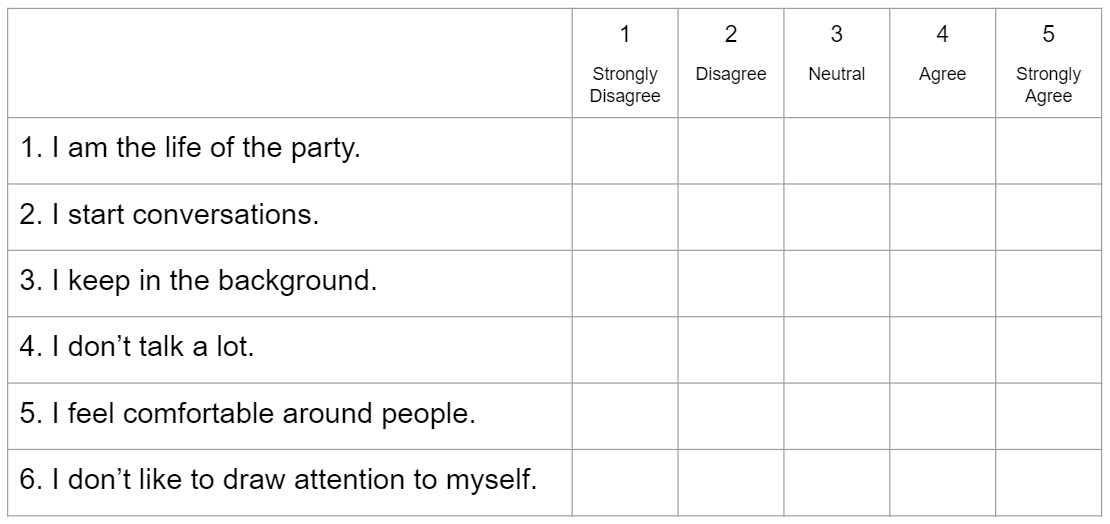
\includegraphics[keepaspectratio]{chapters/images/4_Extraversion.png}}

\subsection{Watch This Video.}\label{watch-this-video.}

\url{https://www.youtube.com/watch?v=W32cHuaWwMU}

\subsection{Check-In}\label{check-in}

\href{https://docs.google.com/forms/d/e/1FAIpQLSdR2QnugvaNWZUptvq8HUitM94pICmsR_17Wiy0LKgmORvZIQ/viewform?usp=sf_link}{PLEASE
COMPLETE THIS CHECK-IN TO PRACTICE REVERSE-SCORING}.

\chapter{Part 2 : Creating a Likert Scale in
R}\label{part-2-creating-a-likert-scale-in-r}

\section{I Like To Read!}\label{i-like-to-read}

In this demonstration, we'll use the class dataset to create a scale to
measure differences in EXTRAVERSION. To do this, we will need to
complete the following steps:

\subsection{1. Import and Check the
Data.}\label{import-and-check-the-data.}

First, we'll need to load the data, and check to make sure it is
imported correctly. You can
\href{https://www.dropbox.com/scl/fi/pz4h809xrhhio25lxc3bo/ec_data.csv?rlkey=0ddbyeid39y21miu2xu04ntnj&dl=0}{access
these data here} - personality measures of extraversion (how social
people say they are) and conscientiousness (how organized people say
they are).

\begin{Shaded}
\begin{Highlighting}[]
\NormalTok{ec }\OtherTok{\textless{}{-}} \FunctionTok{read.csv}\NormalTok{(}\StringTok{"../datasets/ec\_data.csv"}\NormalTok{) }\CommentTok{\# Note: make sure to change the *path* in the \textasciigrave{}read.csv()\textasciigrave{} function to point R to the correct spot to import the ec dataset from YOUR computer.}
\end{Highlighting}
\end{Shaded}

\subsection{2. Create a data.frame that isolates the items in the
scale.}\label{create-a-data.frame-that-isolates-the-items-in-the-scale.}

Now, I'll just create a smaller dataframe of the variables that I want
to work with for the extraversion scale. From the codebook, I see that
the extraversion scale is made up of the items e1-e6r, with the r
indicating items that are negatively-keyed.

\begin{Shaded}
\begin{Highlighting}[]
\NormalTok{extra.df }\OtherTok{\textless{}{-}} \FunctionTok{data.frame}\NormalTok{(ec}\SpecialCharTok{$}\NormalTok{e1, ec}\SpecialCharTok{$}\NormalTok{e2, ec}\SpecialCharTok{$}\NormalTok{e3, }\CommentTok{\# the three positively keyed items}
\NormalTok{                    ec}\SpecialCharTok{$}\NormalTok{e4r, ec}\SpecialCharTok{$}\NormalTok{e5r, ec}\SpecialCharTok{$}\NormalTok{e6r) }\CommentTok{\# the three negatively keyed items}
\FunctionTok{head}\NormalTok{(extra.df) }\CommentTok{\# this code checks my work and make sure my newly created dataframe in fact contain the positively and negatively keyed items}
\end{Highlighting}
\end{Shaded}

\begin{verbatim}
  ec.e1 ec.e2 ec.e3 ec.e4r ec.e5r ec.e6r
1     2     3     2      4      4      4
2     2     4     3      3      3      4
3     3     4     2      4      5      4
4     2     3     2      3      4      3
5     5     5     5      1      1      1
6     1     3     3      3      4      4
\end{verbatim}

\subsection{3. Correctly reverse-score the negatively-keyed items in the
scale.}\label{correctly-reverse-score-the-negatively-keyed-items-in-the-scale.}

Now, I need to reverse-score the negatively keyed items. Since the scale
ranged from 1 to 5, I need to subtract the negatively keyed items from 6
to reverse the scoring (so 6 - 1 = 5, and 6 - 5 = 1.)

\textbf{Note that you can calculate how to reverse-score an item by
adding the lower and upper limit of the full range. So to reverse-score
a response scale that goes from 0 to 4 = 0 + 4 = subtract the negatively
keyed items from 4. A response scale that goes from 1 to 15 = 1 + 15 =
subtract the negatively keyed items from 16. And so on.}

I can again use the head() function to check my work and confirm that I
successfully reverse scored the variables. Note that you can
reverse-score the variables in one step; I don't really do this twice
when creating a scale :)

\begin{Shaded}
\begin{Highlighting}[]
\NormalTok{extra.df }\OtherTok{\textless{}{-}} \FunctionTok{data.frame}\NormalTok{(ec}\SpecialCharTok{$}\NormalTok{e1, ec}\SpecialCharTok{$}\NormalTok{e2, ec}\SpecialCharTok{$}\NormalTok{e3, }\CommentTok{\# the three positively keyed items}
                    \DecValTok{6}\SpecialCharTok{{-}}\NormalTok{ec}\SpecialCharTok{$}\NormalTok{e4r, }\DecValTok{6}\SpecialCharTok{{-}}\NormalTok{ec}\SpecialCharTok{$}\NormalTok{e5r, }\DecValTok{6}\SpecialCharTok{{-}}\NormalTok{ec}\SpecialCharTok{$}\NormalTok{e6r) }\CommentTok{\# the three negatively keyed items}
\FunctionTok{head}\NormalTok{(extra.df) }\CommentTok{\# this code checks my work and make sure my newly created dataframe in fact contain the positively and negatively keyed items. Note that there seems to be more consistency in the scores for each individual {-} people who are low in e1{-}e3 are now also low in e4r {-} e6r.}
\end{Highlighting}
\end{Shaded}

\begin{verbatim}
  ec.e1 ec.e2 ec.e3 X6...ec.e4r X6...ec.e5r X6...ec.e6r
1     2     3     2           2           2           2
2     2     4     3           3           3           2
3     3     4     2           2           1           2
4     2     3     2           3           2           3
5     5     5     5           5           5           5
6     1     3     3           3           2           2
\end{verbatim}

\subsection{4. Evaluate the reliability of the items in this
variable.}\label{evaluate-the-reliability-of-the-items-in-this-variable.}

I'll examine the internal reliability of the scale. Internal reliability
measures how consistent people's responses were for each of the items of
the scale. I'm hoping for a high value.

\begin{Shaded}
\begin{Highlighting}[]
\FunctionTok{library}\NormalTok{(psych) }\CommentTok{\# make sure you install.packages("psych") first!}
\FunctionTok{alpha}\NormalTok{(extra.df)}
\end{Highlighting}
\end{Shaded}

\begin{verbatim}

Reliability analysis   
Call: alpha(x = extra.df)

  raw_alpha std.alpha G6(smc) average_r S/N  ase mean   sd median_r
      0.87      0.87    0.88      0.52 6.6 0.03  3.1 0.88     0.49

    95% confidence boundaries 
         lower alpha upper
Feldt     0.80  0.87  0.92
Duhachek  0.81  0.87  0.92

 Reliability if an item is dropped:
            raw_alpha std.alpha G6(smc) average_r S/N alpha se var.r med.r
ec.e1            0.88      0.88    0.89      0.59 7.2    0.028 0.017  0.58
ec.e2            0.85      0.85    0.85      0.53 5.6    0.035 0.029  0.51
ec.e3            0.82      0.82    0.83      0.48 4.6    0.040 0.025  0.45
X6...ec.e4r      0.85      0.85    0.86      0.53 5.7    0.035 0.032  0.51
X6...ec.e5r      0.80      0.81    0.81      0.46 4.3    0.044 0.020  0.46
X6...ec.e6r      0.86      0.86    0.86      0.55 6.1    0.032 0.020  0.53

 Item statistics 
             n raw.r std.r r.cor r.drop mean   sd
ec.e1       50  0.63  0.63  0.52   0.47  2.9 1.18
ec.e2       50  0.75  0.77  0.72   0.65  3.6 0.91
ec.e3       50  0.87  0.88  0.87   0.79  3.3 1.12
X6...ec.e4r 49  0.77  0.76  0.69   0.64  3.3 1.22
X6...ec.e5r 49  0.91  0.91  0.92   0.86  3.0 1.16
X6...ec.e6r 50  0.73  0.72  0.67   0.59  2.7 1.21

Non missing response frequency for each item
               1    2    3    4    5 miss
ec.e1       0.14 0.26 0.28 0.24 0.08 0.00
ec.e2       0.04 0.06 0.30 0.50 0.10 0.00
ec.e3       0.06 0.20 0.30 0.30 0.14 0.00
X6...ec.e4r 0.04 0.31 0.20 0.24 0.20 0.02
X6...ec.e5r 0.08 0.27 0.35 0.16 0.14 0.02
X6...ec.e6r 0.16 0.34 0.20 0.22 0.08 0.00
\end{verbatim}

\marginnote{\begin{footnotesize}

There's a LOT going on in this code, but I'm looking at the number
underneath raw\_alpha, which shows me that this scale is reliable. This
is good, and would be something that I would report when describing the
measure of Extraversion.

The rest of the code output gives you other statistics on the scale
(e.g., the mean or standard deviation), and shows you what the
reliability of the scale would be if you removed one of the items from
the scale. This can be useful for diagnosing whether there was an issue
with your code (e.g., did you forget to reverse-score one item?) or with
the scale (e.g., is one of your items actually measuring something other
than extraversion?) In this case, the reliability doesn't change much if
we remove any of the items.

\end{footnotesize}}

\subsection{5. Use the rowmeans() function to create a new variable that
is the average of each person's
items.}\label{use-the-rowmeans-function-to-create-a-new-variable-that-is-the-average-of-each-persons-items.}

Now, I need to create one variable that is combines all the items into
one number. To do this, I could either add up each person's 6
extraversion scores, or take the average. The convention is usually to
take the average for personality variables - not sure why\ldots a
cultural difference.

So we will use the rowMeans() function to do this. There are two methods
for this.

\begin{itemize}
\tightlist
\item
  \textbf{Method \#1 (Default - very conservative approach)} : only
  calculate an average score if people answered every item in the
  dataset. This completely removes a person from the dataset, even if
  they answered 5/6 of the questions.
\end{itemize}

{\marginnote{\begin{footnotesize}this calculates the average of these
items for each row (individual) in the dataset. This is the measure of
extraversion for each person. Notice that there is some missing data -
the default for this code is that a person's data will be totally
removed if they didn't answer all the questions in the scale. This is a
very conservative way to handle missing data.\end{footnotesize}}}

\begin{Shaded}
\begin{Highlighting}[]
    \FunctionTok{rowMeans}\NormalTok{(extra.df) }
\end{Highlighting}
\end{Shaded}

\begin{verbatim}
 [1] 2.166667 2.833333 2.333333 2.500000 5.000000 2.333333 3.333333 3.666667
 [9] 2.833333 2.333333 2.000000 3.500000 4.166667 2.333333 4.500000 3.166667
[17]       NA 3.666667 3.000000 3.666667       NA 3.500000 3.666667 4.000000
[25] 1.666667 4.833333 3.666667 3.833333 3.166667 3.000000 2.500000 2.833333
[33] 1.000000 2.833333 3.333333 3.000000 3.166667 2.166667 2.333333 3.166667
[41] 1.833333 3.000000 3.166667 4.333333 4.166667 3.500000 3.500000 2.166667
[49] 4.833333 1.666667
\end{verbatim}

\begin{itemize}
\tightlist
\item
  \textbf{Method \#2 (more liberal approach) :} this removes missing
  data from specific items, so the average score will be calculated even
  if the person didn't answer some of the items.~
\end{itemize}

\begin{Shaded}
\begin{Highlighting}[]
\FunctionTok{rowMeans}\NormalTok{(extra.df, }\AttributeTok{na.rm =}\NormalTok{ T) }\CommentTok{\#     adding na.rm = T as an argument. }
\end{Highlighting}
\end{Shaded}

\begin{verbatim}
 [1] 2.166667 2.833333 2.333333 2.500000 5.000000 2.333333 3.333333 3.666667
 [9] 2.833333 2.333333 2.000000 3.500000 4.166667 2.333333 4.500000 3.166667
[17] 3.800000 3.666667 3.000000 3.666667 2.800000 3.500000 3.666667 4.000000
[25] 1.666667 4.833333 3.666667 3.833333 3.166667 3.000000 2.500000 2.833333
[33] 1.000000 2.833333 3.333333 3.000000 3.166667 2.166667 2.333333 3.166667
[41] 1.833333 3.000000 3.166667 4.333333 4.166667 3.500000 3.500000 2.166667
[49] 4.833333 1.666667
\end{verbatim}

\begin{itemize}
\tightlist
\item
  \textbf{IMPORTANT} In order to save the output as a variable, you will
  need to assign the output of rowMeans() to a new object, ideally one
  that is saved as part of the original dataset.
\end{itemize}

\begin{Shaded}
\begin{Highlighting}[]
\NormalTok{ec}\SpecialCharTok{$}\NormalTok{EXTRAVERSION }\OtherTok{\textless{}{-}} \FunctionTok{rowMeans}\NormalTok{(extra.df, }\AttributeTok{na.rm =}\NormalTok{ T) }\CommentTok{\# this saves the scales to the dataset as a new object (which I\textquotesingle{}m calling EXTRAVERSION). I like to name variables that I create in ALL CAPS. Note that I\textquotesingle{}ve chosen to be less conservative in how I handle missing data.}
\end{Highlighting}
\end{Shaded}

\subsection{6. Graph this variable and interpret the graph (what do you
learn)?}\label{graph-this-variable-and-interpret-the-graph-what-do-you-learn}

Okay, we have a scale! And this scale should measure continuous
variation! Let's graph it. I'm looking for a graph that ranges from 1 to
5 (since that was the limit of my response scale), and something that
looks mostly normally distributed.

\begin{Shaded}
\begin{Highlighting}[]
\FunctionTok{hist}\NormalTok{(ec}\SpecialCharTok{$}\NormalTok{EXTRAVERSION, }\AttributeTok{main =} \StringTok{""}\NormalTok{, }\AttributeTok{col =} \StringTok{\textquotesingle{}black\textquotesingle{}}\NormalTok{, }\AttributeTok{bor =} \StringTok{\textquotesingle{}white\textquotesingle{}}\NormalTok{)}
\end{Highlighting}
\end{Shaded}

\pandocbounded{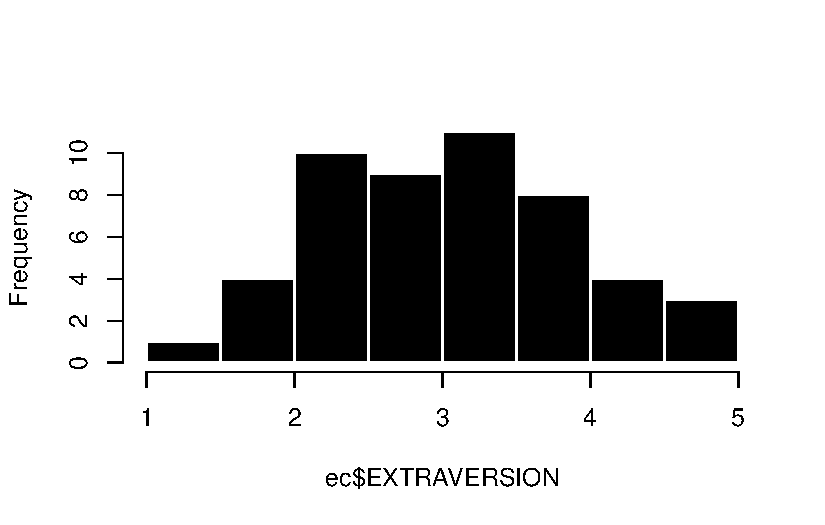
\includegraphics[keepaspectratio]{chapters/4R_Scales_files/figure-pdf/unnamed-chunk-8-1.pdf}}

This looks good. When I look at this graph I see the following things:

\begin{itemize}
\item
  the range of the scale goes from 1 to 5. This is good, because the
  response scale ranged from 1 to 5. An incorrect range would suggest
  that I made a mistake when analyzing the data.
\item
  the graph is mostly normally distributed. This is also good, and
  expected for a personality variable like Extraversion. If there was
  some extreme skew, I might again think that I made a mistake when
  creating the scale, or wonder if there was some non-random variable
  that was influencing students' extraversion scores (for example, the
  entire cohort of students took an improv class during orientation).
\item
  there is some slight positive / right skew - there are a few students
  who are maxed out on extraversion. What's up extraverts {[}waves
  furiously{]}. Not sure why that is, but some deviation from normality
  is always expected! Ooh, one theory is that this survey was given out
  at the end of a three-hour lecture, so maybe students who were more
  extraverted were more likely to stick around in a large classroom
  setting, and thus more likely to be included in the survey. This is an
  example of sampling bias.
\end{itemize}

\section{I Like To Watch Videos : Creating a Likert
Scale}\label{i-like-to-watch-videos-creating-a-likert-scale}

\url{https://youtu.be/TRdDahx6RQw}

\begin{itemize}
\tightlist
\item
  Here's a
  \href{https://www.dropbox.com/s/zsx0shzd3shmpza/likert_scales_c_video.r?dl=0}{link
  to the Rscript} I used in the video
\item
  NOTE : skip / ignore the stuff on using the scale in a model -
  realized that is leftover from when I used to talk about likert scales
  after linear models and prof has not gotten a chance to re-record the
  video\ldots we will talk about linear models in a a few weeks. Let me
  know if you have ideas about how to improve the video for when I do
  re-record!
\end{itemize}

\chapter{Part 3 : Data is Hard in a Soft
Science}\label{part-3-data-is-hard-in-a-soft-science}

One of the challenges psychologists face in their attempts to be a REAL
SCIENCE ™ is that their data is particularly hard to collect. Unlike
physical variables like temperature or mass, psychological variables are
often internal to people, and defined by mental states that are
difficult to observe. As we saw in lecture, even a ``simple'' expressed
behavior like an interruption can be very difficult to measure with high
degrees of reliability and validity that we would hope. For a more
complex variable such as depression, the task might seem impossible.
Indeed, a large part of psychological research is engaging in debate and
scholarship about how to best \textbf{operationalize} variables of
interest (e.g., how should we define or measure depression?)~

A full discussion of the different types of methods psychologists use to
collect data is beyond the scope of this author. However, below I've
tried to outline a few different approaches psychologists take,
commenting on their benefits and limitations so you can begin to
critically think about whether these methods are, in fact, getting at
``THE TRUTH'' of what people (or non-human animals) are like.

\section{Self-Reports}\label{self-reports}

One of the simplest ways to collect data on an individual is just to ask
them what they are like, and have the person report on themselves (a
self-report). There are two different approaches to getting self-reports
- survey methods and qualitative interviews.

\subsection{Qualitative Interviews}\label{qualitative-interviews}

One way to get individuals to tell you what they are like is through a
structured interview where researchers ask open-ended questions. One
such example of this is the McAdams Life Narrative\footnote{McAdams
  talks about his work in this \hyperref[0]{popular press interview} and
  writes about it in this \hyperref[0]{scientific journal review
  article}.}. In this structured interview, a trained research assistant
asks a set of broad questions to participants over the course of 1 to 3
hours. The research assistant is advised to ``feel free to skip some of
these questions if they seem redundant or irrelevant, and should follow
up with other questions as needed `` but also to ``not adopt an advisory
or judgmental role, but should instead serve as an empathic and
encouraging guide and an affirming sounding board.''

Below is an excerpt from the first part of the interview - if you are
comfortable, please share your chapters on the Chapter 4 Discord
thread!\footnote{\href{https://www.dropbox.com/scl/fi/pn3tlz9alo4u0m6lqgcwl/McAdams_Narrative_Instructions.pdf?rlkey=8m48abjh5kgdxbbdworh0dxbh&dl=0}{Here's
  a link to the full narrative instructions} if you want to do the whole
  thing; it's a great way to know someone.}

\pandocbounded{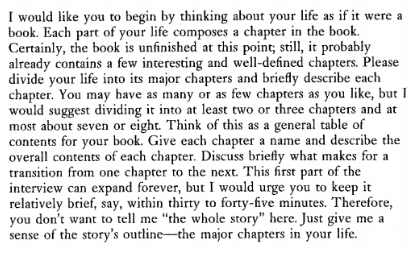
\includegraphics[keepaspectratio]{chapters/images/4_McAdams.png}}

\subsection{Survey Methods}\label{survey-methods}

Qualitative interviews are not very common in psychological research,
because they take a lot of time to conduct, and then more time to
convert people's open-ended responses into data (a form of behavioral
coding, described in more detail below).

Instead, the majority of self-reports come from surveys. Read about
these below.

\begin{longtable}[]{@{}
  >{\raggedright\arraybackslash}p{(\linewidth - 2\tabcolsep) * \real{0.0293}}
  >{\raggedright\arraybackslash}p{(\linewidth - 2\tabcolsep) * \real{0.9707}}@{}}
\toprule\noalign{}
\endhead
\bottomrule\noalign{}
\endlastfoot
\textbf{Definition} & A questionnaire where individuals answer specific
questions about themselves on a structured rating scale. \\
\textbf{Example} & ``On a scale from 1 (Strongly Disagree) to 5
(Strongly Agree), how satisfied with your life are you right now?'' \\
\textbf{Benefits} & \begin{minipage}[t]{\linewidth}\raggedright
\begin{itemize}
\item
  \textbf{Easy to collect :} It only takes a few minutes for people to
  answer a survey, and the data come in a clean and organized format
  that requires little effort to analyze. In Part 2 below, you'll learn
  how to clean and organize the results of a likert scale.
\item
  \textbf{Self-Knowledge Validity :} People know things about
  themselves, often this knowledge is based in ``reality'', and
  sometimes a self-report is the only way to get this knowledge. For
  example, only you know what was your happiest moment in life, and you
  probably have an accurate awareness about how anxious you are about
  the final project in this class.
\end{itemize}
\end{minipage} \\
\textbf{Limitations} & \begin{minipage}[t]{\linewidth}\raggedright
\begin{itemize}
\item
  \textbf{Self-Enhancement / Self-Diminishment Bias :} People are often
  motivated to either enhance or diminish their accomplishments when
  asked. For example, no student has ever come up to me at the end of
  the semester and told me, ``Professor, just so you know - I cheated on
  the exam.'' Even though they may know they cheated, they don't want to
  admit that because our society has norms or guidelines about when
  cheating is appropriate\footnote{Indeed, our society decides what
    \href{https://jacobin.com/2022/11/no-stock-buyback-coalition-labor-unions-corporate-greed-inequality}{forms
    of cheating are acceptable}.}. Other times, a person may not want to
  highlight their accomplishments (self-diminishment) because they don't
  want to seem like they are bragging.
\item
  \textbf{Self-Insight Bias :} Sometimes, people also really don't know
  what they are like. A person may not know, for example, whether they
  snore when they sleep (a behavior), how anxious they really are in a
  situation (an affect), or their patterns of unconscious bias (a
  cognition).
\end{itemize}
\end{minipage} \\
\end{longtable}

Self-reports have a bad reputation in psychology, particularly because
of the ability for people to engage in self-enhancement/diminishment or
self-insight bias. However, they are a very powerful, and very commonly
used method of assessment, even for studies where researchers are able
to observe other types of data.~

For example, despite all the behavioral data that powerful technology
companies like Facebook/Instagram/Meta, TikTok, Twitter/X, etc. collect,
you've probably seen them ask you to answer some survey. They care about
you\footnote{\ldots and your clicking on advertisements; hey, it's hard
  to distinguish the two really\ldots{}}, and know that asking you
questions about yourself is an important way to show that level of care.

Below is one example from some survey when I used to be on Facebook. If
they changed their graphic design since I was last on, it's probably
because of some survey feedback they received.

\begin{center}
\pandocbounded{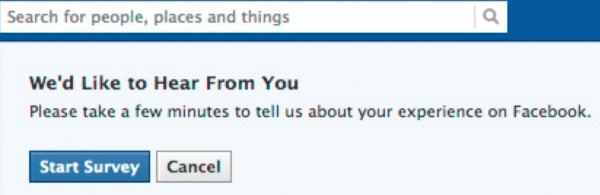
\includegraphics[keepaspectratio]{chapters/images/4L_FBsurvey.png}}
\end{center}

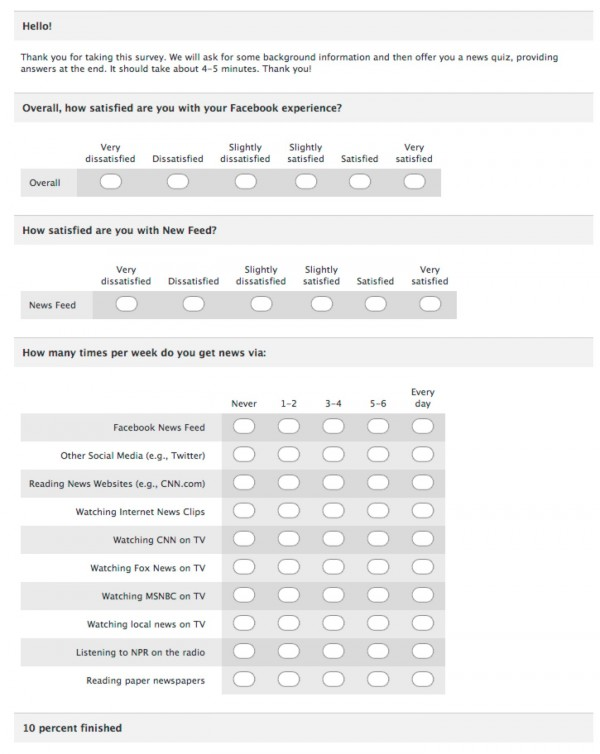
\includegraphics[width=5.46875in,height=\textheight,keepaspectratio]{chapters/images/4L_fbsurvey2.png}

\section{Observations}\label{observations}

Often, self-reports are insufficient to capture what a person is like,
or researchers are studying individuals who cannot give self-reports,
such as infants, people with disabilities, or non-human
animals.\footnote{If I was a billionaire, I'd fund a team of
  psychologists to train monkeys to answer surveys. this is maybe why I
  am not a billionaire. that and the whole ``intergenerational wealth''
  thing / chosen teaching career / lack of a desire to crush others and
  extract as much wealth from them\ldots hard to know which factor is at
  play. Life is complex! Let me know if you are a billionaire and want
  to fund some other ideas / subscribe to my newsletter.

  \hfill\break
}

Read about some common forms of observation methods below.

\begin{longtable}[]{@{}
  >{\raggedright\arraybackslash}p{(\linewidth - 2\tabcolsep) * \real{0.0195}}
  >{\raggedright\arraybackslash}p{(\linewidth - 2\tabcolsep) * \real{0.9805}}@{}}
\toprule\noalign{}
\endhead
\bottomrule\noalign{}
\endlastfoot
\textbf{Definition} & Observational methods refer to ways in which
another individual generates data on the target person of interest. \\
\textbf{Examples} & \begin{minipage}[t]{\linewidth}\raggedright
\textbf{Informant Reports.} Informant reports are a special form of
surveys, where researchers ask friends, family, or strangers to answer
survey questions about another person. This is technically observational
data, since the people answering the surveys are basing their judgments
on their observations of the individual.

\pandocbounded{
\includegraphics[keepaspectratio]{chapters/images/4L_YOU.png}}
\textbar{}

\textbf{Behavioral Data}. When the variables of interest are physical,
then researchers can use measurement tools to directly observe the
behavior. For example, researchers wanting to measure stress might
measure cortisol by taking samples of saliva from the cheek; researchers
wanting to understand the brain look to voxel activation with fMRI, or
cortical neuron activation with EEG.

\pandocbounded{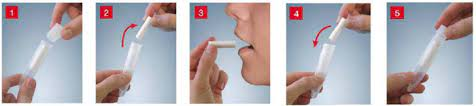
\includegraphics[keepaspectratio]{chapters/images/4L_swab.png}}
\textbar{}

\textbf{Behavioral Coding.} Sometimes, it's easier to have research
assistants observe the physical behaviors of interest. For example,
y'all served as behavioral coders when you counted the number of
interruptions (a behavior!) Other times, research assistants will
observe real-life interactions and observe variables such as time spent
talking, distance between participants, or provide ratings of how much
emotion or anxiety the person seemed to be expressing (using a rating
scale). The ``strange situation'' task (where a parent leaves the room
and researchers observe what a child does) is another
example.\footnote{You can compare
  \href{https://www.youtube.com/watch?v=QquZxJhuSg8}{this child's
  reaction} to \href{https://www.youtube.com/watch?v=AGRT6VjnTm8}{this
  child's reaction}. What do you observe? How would you quantify these
  observations and turn them into cold, hard data?

  \hfill\break
}

\pandocbounded{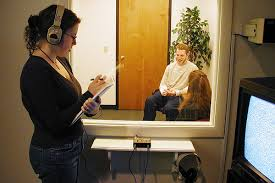
\includegraphics[keepaspectratio]{chapters/images/4_RAnotes.png}}\strut
\end{minipage} \\
\textbf{Benefits} & \begin{minipage}[t]{\linewidth}\raggedright
\begin{itemize}
\item
  \textbf{``External''.} Researchers like observational methods because
  they, by definition, require some outward expression of the underlying
  psychological processes. Professor could go on a rant here and won't,
  but psychology has been increasingly fixated on behavior since Watson
  kicked off the behaviorism movement in the 1920s, and these data are
  often prioritized, since our field loves predicting people's actual
  behavior (so they can exert power over it).
\item
  \textbf{Less influenced by self-report biases.} Observers are
  considered to be less biased than individuals, who may be particularly
  prone to self-enhancement, self-diminishment. And observers may be
  able to fill in the gaps left behind by self-insight bias. For
  example, a person's close friends may know more about the individual's
  reputation than they themselves do.
\item
  \textbf{More reliable (multiple sources).} While there is only one
  self to provide a self-report, there can be multiple observers.
  Indeed, observational methods almost always leverage this power and
  require multiple swabs of spit to get a reliable estimate of cortisol,
  or have multiple research assistants rate the same behavior to check
  and make sure they are each getting a similar answer.
\end{itemize}
\end{minipage} \\
\textbf{Limitations} & \begin{minipage}[t]{\linewidth}\raggedright
\begin{itemize}
\item
  \textbf{Time-Intensive.} It can be incredibly costly to collect
  observational data. Yale charges over \$600/hour for use of their fMRI
  machine (Berkeley doesn't list their prices), and conducting a study
  to measure a naturally occurring behavior could take years between
  designing the study, recruiting and training the research assistants
  to observe the behavior, taking the time to collect the data, and then
  doing the behavioral coding necessary to convert the observations into
  numbers. Whew. Much easier to just give someone a survey and have them
  complete it.
\item
  \textbf{The Hawthorne Effect.} The act of observation can often change
  behavior. Couples may be less likely to fight if they know they are
  being monitored by a psychologist, and even
  \href{https://en.wikipedia.org/wiki/Wave\%E2\%80\%93particle_duality}{light
  changes its behavior depending on the way it is observed}. Researchers
  can take steps to address this change in behavior - and sometimes the
  power of the phenomenon is so large that it doesn't matter if a
  researcher is there. In couples studies, for example, researchers can
  get couples to fight by having each person write out a list of things
  that cause conflict in the relationship, and then having the people
  trade lists and talk about it. Often however, individuals habituate to
  the presence of observation - do you think about the fact that your
  online interactions are being harvested by tech companies every day,
  or just kinda get used to it?
\item
  \textbf{Not all aspects of psychology are observable.} A person's
  subjective experience matters, and sometimes a self-report is the only
  way you can get this data. If you look like you are smiling and have
  the neurotransmitter levels that suggest you are happy, but feel
  miserable, are you happy?
\end{itemize}
\end{minipage} \\
\end{longtable}

\textbf{TLDR : there are lots of different methods to measure what
individuals are like, and for your final project you probably will want
to give people self-report surveys to keep things simple for this very
first study!}

\chapter{Quiz 4.}\label{quiz-4.}

Note : Creating likert scales takes practice. So I went ahead and
uploaded a video key for Quiz 4 (as part of the quiz assignment). You
should try to take the quiz on your own - good to have a little bit of
struggle! - and use the video key as a guide to learn. We will continue
to practice over the next few weeks; this is the last new big topic in R
we will learn before the R Exam.

\chapter{``Normal'' Data}\label{normal-data}

In this chapter, we'll define and discuss the idea of ``normality'', how
psychologists (and scientists) evaluate whether data are ``good''.

\pandocbounded{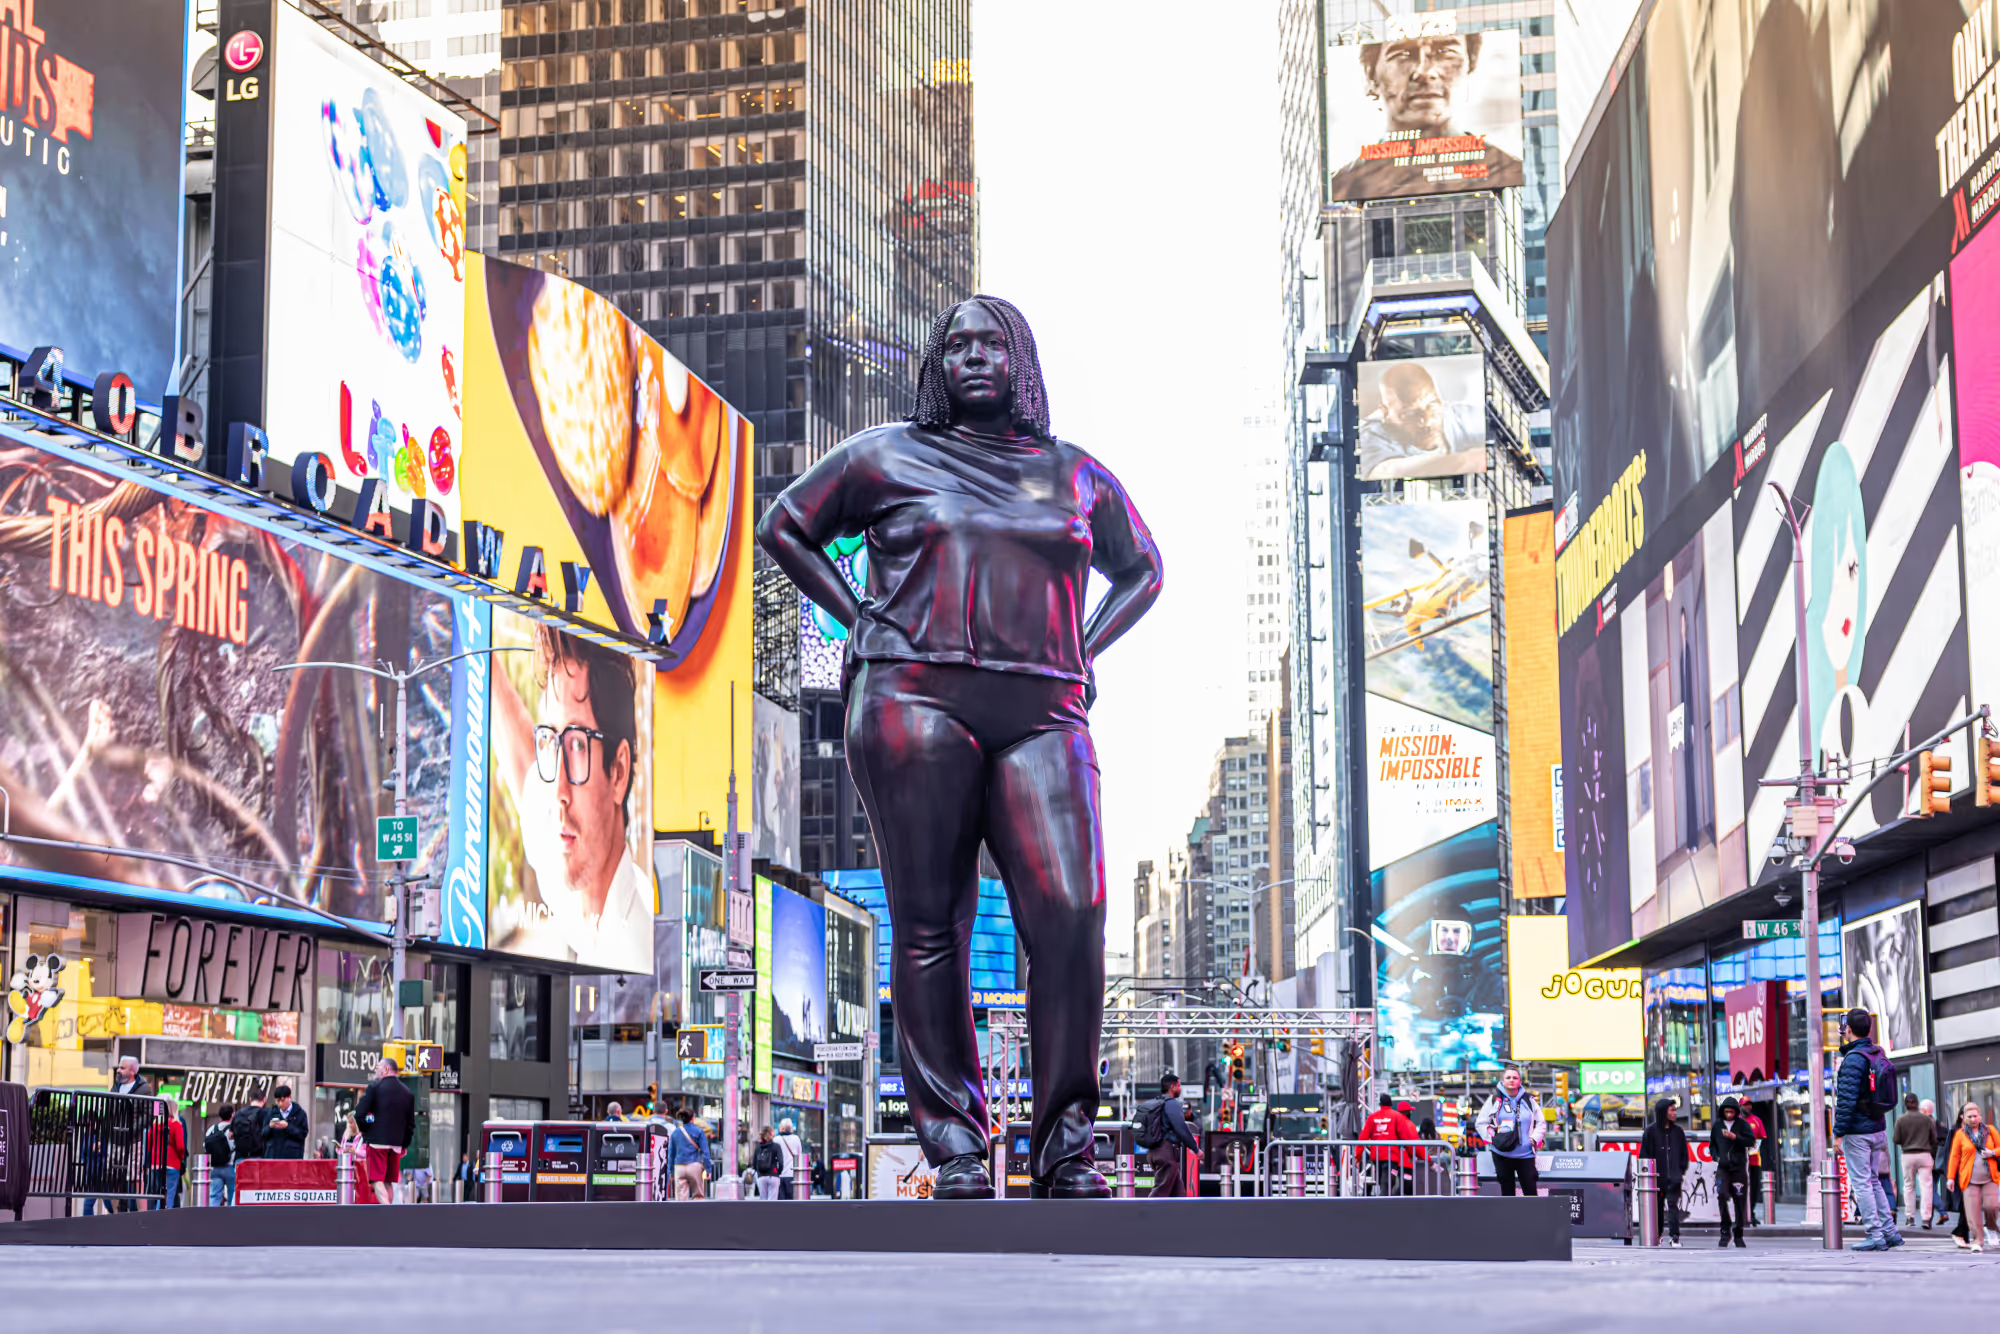
\includegraphics[keepaspectratio]{chapters/images/clipboard-4149537892.png}}

The image above depicts
\href{https://www.thomasjprice.com/times-square-arts}{\emph{Grounded in
the Stars}}, a 12-foot sculpture of a young woman that stood in New York
CIty's Times Square from April 29 through June 14, 2025.

There's a lot that I love about this image, from the artistry of
rendering braids and clothes so naturally in sculpted bronze, to the way
the character stares off in the distance as if unconcerned with the gaze
of others, to the way the sculpture proudly claims space in a society
that does not currently and historically create inclusive spaces for
black women. Indeed, the sculpture is surrounded by other massive
images\footnote{Tom Cruise and some eyeglass model who kind of looks
  like a 90s era Tom Cruise. Ving Rhames is there too if you look
  closely enough.} whose presence in the space may go unnoticed because
it is so routine to see images of white men in public places.

The artist's website emphasizes the way the sculpture challenges
pre-existing ideas about who is represented in our society, and
references Michelangelo's \emph{David} as inspiration, but clarifies
that this sculpture is ``A fictionalized character constructed from
images, observations, and open calls spanning between Los Angeles and
London'' who ``carries familiar qualities, from her stance and
countenance to her everyday clothing.''

This statue, and the fact that it was an amalgamation of real people,
also reminded me of the sculptures of ``Normmann'' and Norma.

\marginnote{\begin{footnotesize}

\pandocbounded{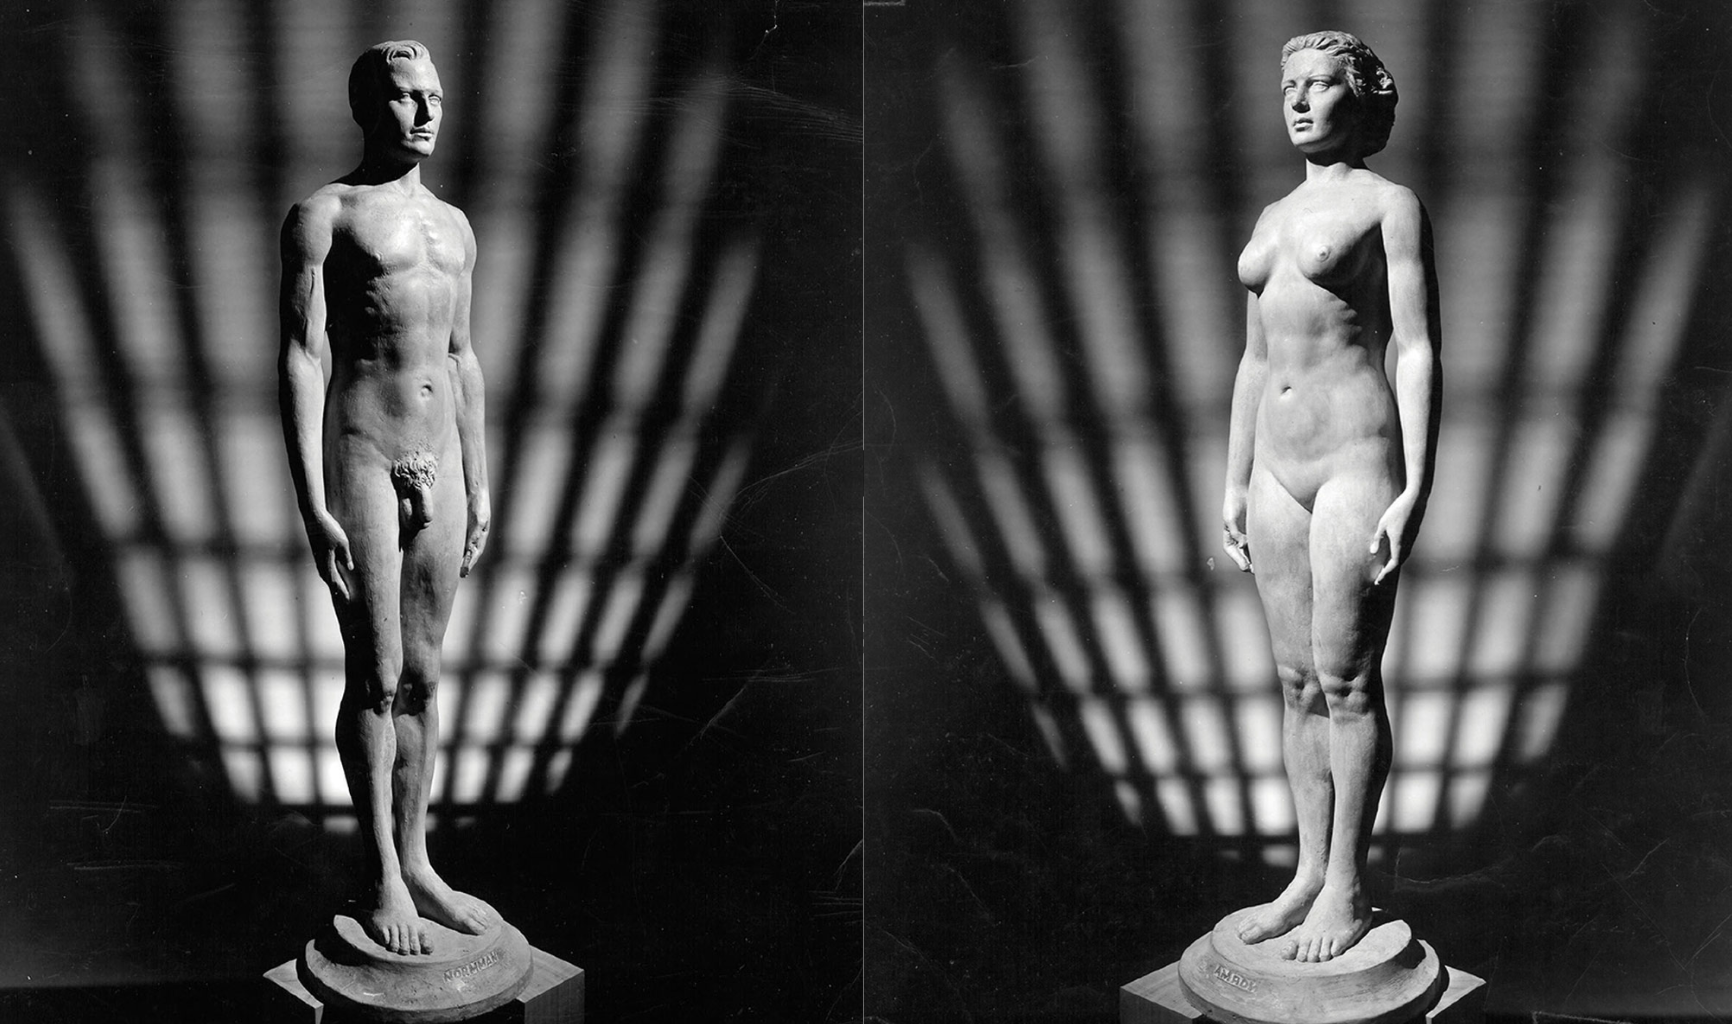
\includegraphics[keepaspectratio]{chapters/images/clipboard-1894112951.png}}

\end{footnotesize}}

Like the unnamed woman in Times Square who was the subject of
\emph{Grounded in the Stars,} Normmann and Norma's measurements were
based on composites of other people; in Norma's case ``the averaged
measurements of `native white' American women recorded and standardized
by the Bureau of Home Economics in 1940, in an attempt to devise the
first standardized system of sizing for ready-made clothes.''\footnote{For
  a more in-depth history of Norma and Normann, including critiques of
  the gender and post-WW2 contexts in which these statues arose, See
  Chapter 8 of Peter Cryle \& and Elizabeth Stephens' \emph{Normality: A
  Critical Genealogy}. University of Chicago Press, 2017.Chicago
  Scholarship Online, 2018.
  \hyperref[0]{https://doi.org/10.7208/chicago/9780226484198.001.0001}.}

Unlike the subject of \emph{Grounded in the Stars,} Norma and Normmann
were based on different demographic data. More important, these
characters were labeled and advertised as ``The Typical American''. A
type of person who reflected and reinforced the values that white
America wanted to promote.

Indeed, these statues achieved their purpose in various ways; Norma and
Normman were first displayed in the American Museum of Natural History
during the International Congresses of Eugenics in 1945. Furthermore,
when the statues were gifted to the Cleveland Health Museum, the museum
held a contest to find the woman who most typically represented
Norma\footnote{I'm not entirely sure why Normann was not subject to a
  similar contest, though my guess is that it's a symptom of a
  patriarchy that perpetuates the male gaze in
  \href{https://www.youtube.com/watch?v=ulsjuiFO2J0}{many ways}.},
offering prize money in ``a search for Norma, the typical American
woman''. While a winner was selected, the search failed in the original
efforts to find someone who \emph{perfectly} matched this average, as
the measurements of the winner ``did not coincide with those of the
statue. . . . after assessment of the measurements of 3,863 women who
entered the search, Norma remained a hypothetical
individual.''\footnote{Josephine Robertson, ``Theatre Cashier, 23, Wins
  Title of `Norma,' Besting 3,863 Entries,'' Cleveland Plain Dealer,
  September 23, 1945, 1.}

Here, we see a few course themes that we will discuss in this chapter,
and in this week's lecture :

\begin{itemize}
\item
  What is ``normal'' and who gets to define this term?
\item
  What are the alternatives to ``normality''? How are these alternatives
  labeled?
\item
  What is the point of labeling individuals as normal?
\end{itemize}

\chapter{Part 1. The ``Normal''
Distribution.}\label{part-1.-the-normal-distribution.}

Before we get into the critique in our class, let's use this space to go
over some of the basic definitions.

\section{Definition.}\label{definition.-3}

The ``Normal'' (or Gaussian) distribution is a common shape for what
distributions of data look like. The shape is often called a ``bell
curve'', because it looks like the curve of a bell. Ding.

While many distributions appear normal, the ``Normal Distribution'' ™
refers to a distribution that describes an expected probability of a
range of scores.

\begin{center}
\pandocbounded{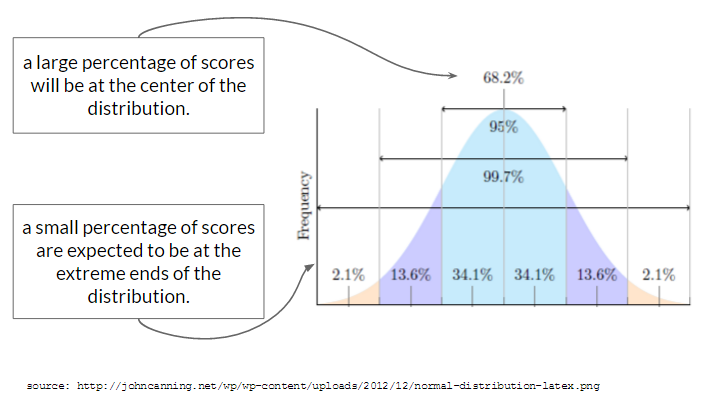
\includegraphics[keepaspectratio]{chapters/images/3_NormalDistributionAnnotated.png}}
\end{center}

The Normal Distribution is called ``normal'', in part, because
researchers expect to see this type of distribution for variables where
two conditions are met:

\begin{enumerate}
\def\labelenumi{\arabic{enumi}.}
\tightlist
\item
  \textbf{There are multiple explanations for why the variation occurs}.
  This happens very frequently across all science, since life is complex
  and there are many reasons why individuals differ.
\item
  \textbf{These multiple explanations occur independently}.
  ``Independence'' means that one explanation for variation is unrelated
  to the presence of another explanation for variation. For example,
  your height is somewhat influenced by your genetics (you are likely
  similar height to your family members) and your diet (i.e., whether
  you got enough nutrients in childhood or not), but your diet is likely
  unrelated to your genetics. Non-independence might mean that there is
  some shared experience among individuals that is influencing their
  variation in predictable ways. For example, children who were exposed
  to all the horrors of war experienced multiple factors that negatively
  impacted their height - malnutrition, sleep disturbances,
\end{enumerate}

Indeed, many of the variables that psychologists measure do appear
``Normal''. For example, let's look at one example ``normal''
distributions - the ``self-esteem'' variable we saw in Lecture 2. Note
that it's not perfectly normal\footnote{good not to hold data to
  unrealistic body images as well as people.}, but it's pretty close and
representative of the kind of ``real world'' data that you might
encounter.

\begin{Shaded}
\begin{Highlighting}[]
\FunctionTok{hist}\NormalTok{(d}\SpecialCharTok{$}\NormalTok{SELFES, }\AttributeTok{col =} \StringTok{\textquotesingle{}black\textquotesingle{}}\NormalTok{, }\AttributeTok{bor =} \StringTok{\textquotesingle{}white\textquotesingle{}}\NormalTok{, }
     \AttributeTok{main =} \StringTok{"Histogram of Self{-}Esteem"}\NormalTok{, }
     \AttributeTok{xlab =} \StringTok{"Self{-}Esteem Score"}\NormalTok{, }\AttributeTok{breaks =} \DecValTok{15}\NormalTok{)}
\end{Highlighting}
\end{Shaded}

\pandocbounded{\includegraphics[keepaspectratio]{chapters/5R_GoodScience_files/figure-pdf/unnamed-chunk-2-1.pdf}}

\textbf{``Independent'' explanations for why variation in self-esteem
occurs.} Self-esteem is complex, and can be influenced by variables such
as: genetics, parental environment, home environment, income,
neurotransmitters, whether your crush told you they like you too the day
you took the self-esteem survey, etc. These variables are considered
independent because one does not influence the other, and they differ
across participants in the study. That is, someone who had a happy
parental environment may not necessarily have a high income, rich people
have their crushes ignore them too, etc.

\textbf{``Non-Random'' Explanations.} Careful observers will note that
self-esteem appears slightly shifted above the mid-point of the scale
(which goes from 1-4, so 2.5 would be the mid-point), and that there's
some slight negative skew (meaning more individuals are on the higher
end of the distribution). It's unclear why there's this shift in the
data, but below are a few possible reasons :

\begin{itemize}
\item
  There's some shared cultural experiences among participants - our
  society values self-esteem, and people might be biased to self-enhance
  / self-present a higher self-esteem. This is a non-independent
  influence, since many participants might experience this in our
  culture that puts pressure on people to have a high self-esteem.
\item
  The sample was biased to include people with higher levels of
  self-esteem, or maybe people with lower levels of self-esteem were
  less likely to complete the survey (which hurts their self-esteem
  because they haven't yet fully internalized that it's okay to be
  imperfect in a society that demands perfection.) In any case
\item
  The survey was administered on a day when everyone in the world had a
  really good hair day, so there's a non-independent factor that's
  shifting many people's self-esteem up.
\end{itemize}

\subsection{Example 2 : Thinking About
Distributions}\label{example-2-thinking-about-distributions}

Below is another example of a distribution - this one is not random, but
is skewed (pop quiz : is it positively or negatively skewed? See here
for answer\footnote{It is negatively skewed, since the tail is on the
  negative side of the distribution.}.)

\begin{center}
\pandocbounded{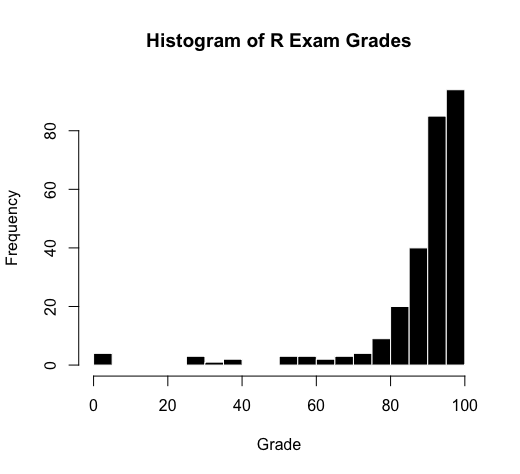
\includegraphics[keepaspectratio]{chapters/images/3_RGrades.png}}
\end{center}

\begin{tcolorbox}[enhanced jigsaw, toptitle=1mm, toprule=.15mm, rightrule=.15mm, breakable, left=2mm, colbacktitle=quarto-callout-tip-color!10!white, colback=white, opacityback=0, coltitle=black, bottomtitle=1mm, opacitybacktitle=0.6, titlerule=0mm, leftrule=.75mm, arc=.35mm, bottomrule=.15mm, title=\textcolor{quarto-callout-tip-color}{\faLightbulb}\hspace{0.5em}{``Random'' Reasons for Variation}, colframe=quarto-callout-tip-color-frame]

Lots of things can influence a student's score on an exam, such as how
much students were motivated to study, how much time they had to study,
what was going on in their lives, whether they had a study buddy in the
class, whether they were sick or not on the day of the exam, their
``test taking'' skills and strategies and anxiety levels, etc.

\end{tcolorbox}

\begin{tcolorbox}[enhanced jigsaw, toptitle=1mm, toprule=.15mm, rightrule=.15mm, breakable, left=2mm, colbacktitle=quarto-callout-tip-color!10!white, colback=white, opacityback=0, coltitle=black, bottomtitle=1mm, opacitybacktitle=0.6, titlerule=0mm, leftrule=.75mm, arc=.35mm, bottomrule=.15mm, title=\textcolor{quarto-callout-tip-color}{\faLightbulb}\hspace{0.5em}{``Non-Random'' Reasons for Variation.}, colframe=quarto-callout-tip-color-frame]

These data are not normally distributed because the students were all
part of the same college, in the same classroom, taught by the same
professor, at the same time. The professor did his best to prepare these
students, and wrote a test that would be based on the kinds of practice
they had gone over in lecture. These variables are considered ``non
random'' because they were shared by all students. The data are skewed
because these non-random shared experiences helped students do well on
the exam.

\end{tcolorbox}

\subsubsection{}\label{section}

\marginnote{\begin{footnotesize}

\includegraphics[width=3in,height=\textheight,keepaspectratio]{chapters/../images/doff_intro_mickey.png}

\end{footnotesize}}

\begin{tcolorbox}[enhanced jigsaw, toptitle=1mm, toprule=.15mm, rightrule=.15mm, breakable, left=2mm, colbacktitle=quarto-callout-warning-color!10!white, colback=white, opacityback=0, coltitle=black, bottomtitle=1mm, opacitybacktitle=0.6, titlerule=0mm, leftrule=.75mm, arc=.35mm, bottomrule=.15mm, title=\textcolor{quarto-callout-warning-color}{\faExclamationTriangle}\hspace{0.5em}{Culture in Statistics : The Normal Curve}, colframe=quarto-callout-warning-color-frame]

That's right folks, it's time for another chat with your friend
Open-Source Mickey Mouse! This time, we're gonna chat about the idea
that people differ from some average. The idea that you could quantify
people as ``average'' is fairly new - it's hard to pinpoint exactly, but
a scientist named Quetelet first extended the statistical methods
derived from astronomy to be applied to humans in the
1860s\footnotemark{}. Quetelet thought the average was an ideal state
since it reflected the center of all possible individuals. However, a
few years later Francis Galton used Quetelet's ideas to try and ``rank''
individuals according to some hierarchy of excellence. For Galton, the
average was not an ideal state, but rather something to overcome in a
desire for greater and greater excellence. Galton was also a racist and
father of the eugenics movement, who used distorted statistics as a tool
to justify his own pre-existing racist beliefs that white people were
superior to everyone else. Yuck!

I think it's worth the time and space to hear this from Galton himself.

\emph{To conclude, the range of mental power between---I will not say
the highest Caucasian and the lowest savage---but between the greatest
and least of English intellects, is enormous. \ldots{} I propose in this
chapter to range men according to their natural abilities, putting them
into classes separated by equal degrees of merit, and to show the
relative number of individuals included in the several
classes\ldots..The method I shall employ for discovering all this, is an
application of the very curious theoretical law of ``deviation from an
average.'' First, I will explain the law, and then I will show that the
production of natural intellectual gifts comes justly within its scope.
-} Galton, Hereditary Genius (1869).
\href{https://galton.org/books/hereditary-genius/text/v5/galton-1869-hereditary-genius-v5.htm}{Linked
here}.

The point of bringing up some of the racist origins of statistics is
two-fold :

\begin{enumerate}
\def\labelenumi{\arabic{enumi}.}
\tightlist
\item
  Many people like to argue that ``good'' statistics is objective, and
  that scientists are free of bias. So it's important to acknowledge
  that the inventors of many statistics that we use had clear biases and
  did not behave objectively. Rather than try to be free of bias, I
  think it's important to acknowledge where and when people are biased,
  and address those biases up explicitly.
\item
  Statistics is a tool, and that tool can be used poorly and dangerously
  in ways that can cause a lot of pain. Just because something has
  numbers doens't mean it's correct. For example, Galton's work showing
  ``statistically'' that white people were superior in ability to other
  groups didn't account for other factors like socioeconomic status. And
  for what it's worth, modern scientists overwhelmingly agree that
  ``race'' is a social construct. There are genetic differences that
  explain different skin tones, however there is more genetic variation
  in skin tone within a similar ``race'' than between different
  ``races''.
  \href{https://www.smithsonianmag.com/smart-news/genetic-study-shows-skin-color-just-skin-deep-180965261/}{Read
  more about this here.}
\end{enumerate}

Alright, that's all for now! Let me know what you think and see you next
time!

\end{tcolorbox}

\footnotetext{see Rose's END OF AVERAGE (2016) or, for a more critical
approach, Chapman's (2023) EMPIRE OF NORMALITY.}

\section{Why This Matters.}\label{why-this-matters.}

The normal distribution is foundational to the statistics we will learn
in this class. (And in an advanced statistics class, you'll learn how to
adapt techniques if you want to understand non-normal distributions.)

This does not mean that every variable needs to be normally distributed;
we'll work with skewed variables and categorical variables (which have
their own distributions) in lots of ways. However, the ``normal
distribution'' is an important reference point that we can use to
evaluate variables. For example, exam scores are \emph{negatively
skewed} because they differ from the normal distribution.

\chapter{Part 2. Outliers and Z-Scoring in
R}\label{part-2.-outliers-and-z-scoring-in-r}

\section{Some Conceptual
Understanding}\label{some-conceptual-understanding}

\subsection{Z-Score : Definition}\label{z-score-definition}

The z-score is a linear transformation\footnote{A linear transformation
  means that the order and spacing of the data are unchanged - the
  person who has the highest self-esteem when measured on a 0 to 4 scale
  will still have the highest z-score, and be the same distance away
  from the next highest individual.} that calculates the distance of an
individual score (\({y_i}\)) from the mean (\(\hat{y}\)) in units of
standard deviation \({\sigma_y}\).

\[
\huge z = \frac{y_i - \hat{y}}{\sigma_y}
\]

Each individual score in the dataset can be z-scored, and this statistic
tells you how far above or below the individual is from others (the
mean), relative to the average difference from the means (which is what
the standard deviation describes.)

Z-scoring changes the units of the variable from the original unit of
measurement, to units of standard deviation.

\begin{itemize}
\item
  A z-score of 1 means that the individual is 1 standard deviation above
  the mean (about as different as average).
\item
  A z-score of 0 means that the individual is EXACTLY the mean.
\item
  A z-score of -4.112 means that the individual is over 4 standard
  deviations below the mean; which is VERY below average.
\item
  A z-score of .01 means the person is just a tiiiiny bit above the
  mean.
\end{itemize}

\subsection{Z-Score : in R}\label{z-score-in-r}

You can see first few ``Raw'' and ``Z-Scores'' from the self-esteem
dataset below.

\begin{verbatim}
  Raw.Scores   Z.Scores
1        3.0  0.5300156
2        3.3  0.9593493
3        2.4 -0.3286517
4        2.7  0.1006820
5        4.0  1.9611279
6        3.6  1.3886830
\end{verbatim}

There are two ways of calculating the z-scores:

\begin{enumerate}
\def\labelenumi{\arabic{enumi}.}
\item
  \textbf{Using the \texttt{scale()} function.} This function calculates
  the mean and standard deviation of an object, and then uses these
  statistics to calculate the z-score for the data.

\begin{Shaded}
\begin{Highlighting}[]
\NormalTok{d}\SpecialCharTok{$}\NormalTok{SELFES\_Z }\OtherTok{\textless{}{-}} \FunctionTok{scale}\NormalTok{(d}\SpecialCharTok{$}\NormalTok{SELFES)}
\NormalTok{d}\SpecialCharTok{$}\NormalTok{SELFES\_Z[}\DecValTok{1}\SpecialCharTok{:}\DecValTok{5}\NormalTok{]}
\end{Highlighting}
\end{Shaded}

\begin{verbatim}
[1]  0.5300156  0.9593493 -0.3286517  0.1006820  1.9611279
\end{verbatim}

  \begin{itemize}
  \tightlist
  \item
    Note that the {[}1:5{]} index is not needed for z-scoring, and is
    just helping me only show the first five elements.
  \end{itemize}
\item
  \textbf{You can also manually calculate a z-score.} But don't do this
  by hand. I mean you could, but you could also do this with a pencil
  and that's not needed anymore.

\begin{Shaded}
\begin{Highlighting}[]
\NormalTok{zSELF }\OtherTok{\textless{}{-}}\NormalTok{ (d}\SpecialCharTok{$}\NormalTok{SELFES }\SpecialCharTok{{-}} \FunctionTok{mean}\NormalTok{(d}\SpecialCharTok{$}\NormalTok{SELFES, }\AttributeTok{na.rm =}\NormalTok{ T)) }\SpecialCharTok{/} \CommentTok{\# distance from the mean, divided by....}
          \FunctionTok{sd}\NormalTok{(d}\SpecialCharTok{$}\NormalTok{SELFES, }\AttributeTok{na.rm =}\NormalTok{ T) }\CommentTok{\# the standard deviation}
\NormalTok{zSELF[}\DecValTok{1}\SpecialCharTok{:}\DecValTok{5}\NormalTok{] }\CommentTok{\# just showing the first 10 z{-}scored variables.}
\end{Highlighting}
\end{Shaded}

\begin{verbatim}
[1]  0.5300156  0.9593493 -0.3286517  0.1006820  1.9611279
\end{verbatim}
\end{enumerate}

\subsection{Z-Score : Who Cares?}\label{z-score-who-cares}

A z-score can be useful for two reasons :

\begin{enumerate}
\def\labelenumi{\arabic{enumi}.}
\tightlist
\item
  \textbf{It removes the units of measurement.} Many variables in
  psychology are measured with likert scales, or other made up numbers
  that don't have a shared meaning, but are instead meant to rank or
  sort individuals along some spectrum. For example, I don't really know
  what to do with the knowledge that a person 3 in the dataset has a
  self-esteem score of 2.4 . But knowing that this person's z-score is
  -0.3286517 tells me that their self-esteem is lower than average, but
  only a little lower than the average.
\item
  \textbf{It emphasizes the individual's rank within the distribution.}
  If you know a job at Amazon dot com is offering 5187 BEZOS BUCKS, you
  may not know whether this is a high or low paying job among other jobs
  at Amazon dot com. But if you know the salary of this job has a
  z-score of .34, you know that this job is higher than average, but
  only a little higher.
\end{enumerate}

\section{Example : Using Z-Scores to Make Decisions About
Outliers}\label{example-using-z-scores-to-make-decisions-about-outliers}

If we look at the variable age from the same self-esteem dataset, we see
some issues.

\begin{Shaded}
\begin{Highlighting}[]
\FunctionTok{hist}\NormalTok{(d}\SpecialCharTok{$}\NormalTok{age)}
\end{Highlighting}
\end{Shaded}

\pandocbounded{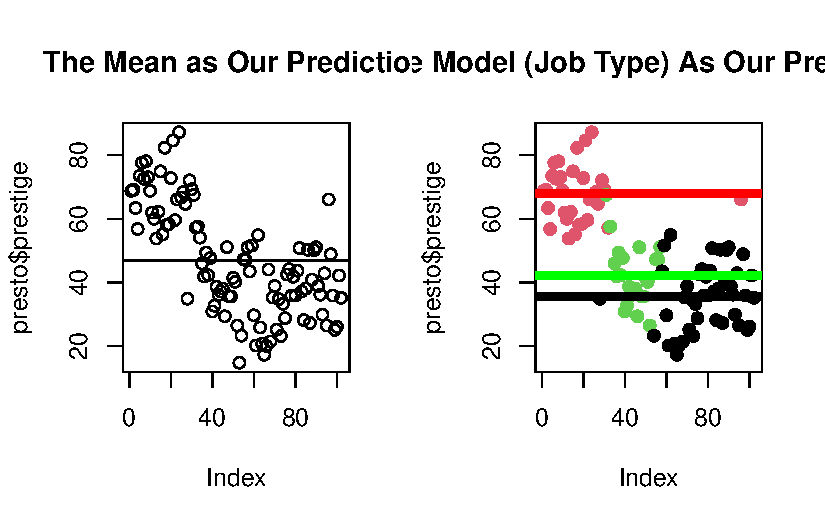
\includegraphics[keepaspectratio]{chapters/5R_GoodScience_files/figure-pdf/unnamed-chunk-6-1.pdf}}

This looks wrong. R says this is a histogram, but it doesn't look like
the histograms we've seen before for a few reasons :

\begin{enumerate}
\def\labelenumi{\arabic{enumi}.}
\tightlist
\item
  \textbf{Why does the x-axis go so far to the right?} There are extreme
  outliers in the variable age - most likley due to errors in data entry
  - that are way out to the right on the x-axis.
\item
  \textbf{What are those numbers on the x-axis!?} These outliers are so
  extreme, that R is reporting the values of age using exponents. 5e+08
  means 5 * 10\^{}8 = 5 * 10 * 10 * 10 * 10 * 10 * 10 * 10 * 10 =
  500,000,000 = 500 million. Whew!
\item
  \textbf{But where are these outliers on the graph? It doesn't look
  like there's anything there?} The dataset is so large (tens of
  thousands of people appear to have ages that are closer to zero years
  old than 500 million years old) that the individual outliers are not
  registering on the graph. But they exist, and we can use R to find
  them.
\end{enumerate}

\begin{Shaded}
\begin{Highlighting}[]
\NormalTok{d}\SpecialCharTok{$}\NormalTok{age[d}\SpecialCharTok{$}\NormalTok{age }\SpecialCharTok{\textgreater{}} \DecValTok{100} \SpecialCharTok{\&} \SpecialCharTok{!}\FunctionTok{is.na}\NormalTok{(d}\SpecialCharTok{$}\NormalTok{age)]}
\end{Highlighting}
\end{Shaded}

\begin{verbatim}
 [1]       1975       1993        229        366       1354      90210
 [7]      80230        120        590        442        234        258
[13]        333        980       1000      45678        333        156
[19]        134        152        474        414        334        630
[25]        169       1997 2147483647        123       7300        118
[31]        972       9000     100000        662        117
\end{verbatim}

In this code, I'm using indexing {[}{]} to ask R to find two things :

\begin{itemize}
\item
  \texttt{d\$age\ \textgreater{}\ 120} asks R to find the rows from the
  dataset d that contain ages that are greater than 100 years old.
\item
  \textbf{\texttt{!is.na(d\$age)}} asks R to find the rows where age is
  NOT and NA values (the ! when used in coding means ``not''). You don't
  strictly need this code, but it made the output easier to read by
  removing all the NA values that I don't care about right now.
\item
  the \texttt{\&} sign in between these commands asks R to find
  individuals where both conditions are met. You can also use the
  \texttt{\textbar{}} bar\footnote{the bar can be typed by hitting shift
    + the key above your return or enter key on the keyboard.} to ask R
  to find individuals where EITHER condition is met.
\end{itemize}

I see that some of the ages were entered in as the year of birth; others
look like maybe errors in data entry or jokes (e.g., 90210) and someone
entered in an extreme value of 2147483647 that is contributing to our
strange graph, and throwing off the mean (but not the median, since it,
as we all remember from Chapter 3, is less sensitive to outliers.)

\begin{Shaded}
\begin{Highlighting}[]
\FunctionTok{mean}\NormalTok{(d}\SpecialCharTok{$}\NormalTok{age, }\AttributeTok{na.rm =}\NormalTok{ T)}
\end{Highlighting}
\end{Shaded}

\begin{verbatim}
[1] 45333.77
\end{verbatim}

\begin{Shaded}
\begin{Highlighting}[]
\FunctionTok{median}\NormalTok{(d}\SpecialCharTok{$}\NormalTok{age, }\AttributeTok{na.rm =}\NormalTok{ T)}
\end{Highlighting}
\end{Shaded}

\begin{verbatim}
[1] 22
\end{verbatim}

\subsection{Side Quest : Removing Outliers Without
Z-Scoring}\label{side-quest-removing-outliers-without-z-scoring}

So let's remove these outliers, and check to see that R did this
correctly.

\begin{Shaded}
\begin{Highlighting}[]
\NormalTok{d}\SpecialCharTok{$}\NormalTok{age[d}\SpecialCharTok{$}\NormalTok{age }\SpecialCharTok{\textgreater{}} \DecValTok{100} \SpecialCharTok{\&} \SpecialCharTok{!}\FunctionTok{is.na}\NormalTok{(d}\SpecialCharTok{$}\NormalTok{age)] }\CommentTok{\# finds the outliers}
\end{Highlighting}
\end{Shaded}

\begin{verbatim}
 [1]       1975       1993        229        366       1354      90210
 [7]      80230        120        590        442        234        258
[13]        333        980       1000      45678        333        156
[19]        134        152        474        414        334        630
[25]        169       1997 2147483647        123       7300        118
[31]        972       9000     100000        662        117
\end{verbatim}

\begin{Shaded}
\begin{Highlighting}[]
\NormalTok{d}\SpecialCharTok{$}\NormalTok{age[d}\SpecialCharTok{$}\NormalTok{age }\SpecialCharTok{\textgreater{}} \DecValTok{100} \SpecialCharTok{\&} \SpecialCharTok{!}\FunctionTok{is.na}\NormalTok{(d}\SpecialCharTok{$}\NormalTok{age)] }\OtherTok{\textless{}{-}} \ConstantTok{NA} \CommentTok{\# replaces the outliers with NA}
\FunctionTok{hist}\NormalTok{(d}\SpecialCharTok{$}\NormalTok{age) }\CommentTok{\# my graph.}
\end{Highlighting}
\end{Shaded}

\pandocbounded{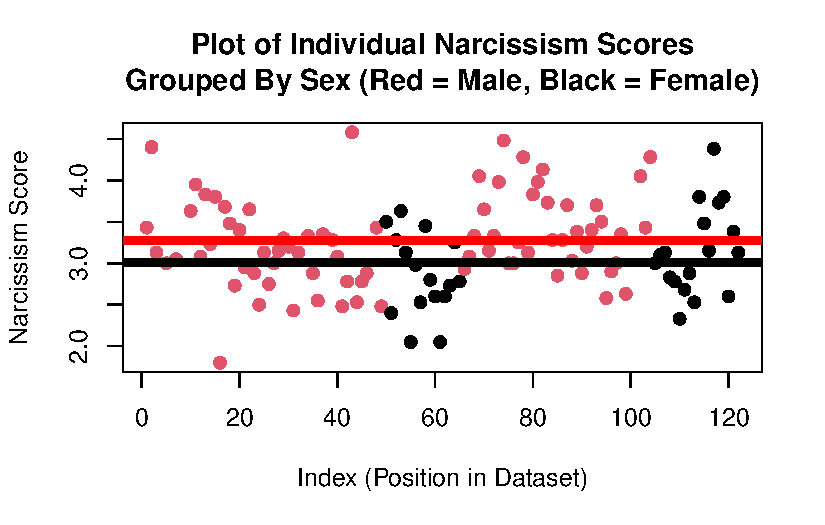
\includegraphics[keepaspectratio]{chapters/5R_GoodScience_files/figure-pdf/unnamed-chunk-9-1.pdf}}

This looks better, but now I see that there are some suspiciously young
ages.

So I'll adapt my code to look for individuals who are less than 18 years
old.

\begin{Shaded}
\begin{Highlighting}[]
\FunctionTok{min}\NormalTok{(d}\SpecialCharTok{$}\NormalTok{age, }\AttributeTok{na.rm =}\NormalTok{ T)}
\end{Highlighting}
\end{Shaded}

\begin{verbatim}
[1] 1
\end{verbatim}

\begin{Shaded}
\begin{Highlighting}[]
\NormalTok{youngfolk }\OtherTok{\textless{}{-}}\NormalTok{ d}\SpecialCharTok{$}\NormalTok{age[d}\SpecialCharTok{$}\NormalTok{age }\SpecialCharTok{\textless{}} \DecValTok{18} \SpecialCharTok{\&} \SpecialCharTok{!}\FunctionTok{is.na}\NormalTok{(d}\SpecialCharTok{$}\NormalTok{age)] }
\NormalTok{youngfolk[}\DecValTok{1}\SpecialCharTok{:}\DecValTok{100}\NormalTok{] }\CommentTok{\# just the first 100 folks less than 18}
\end{Highlighting}
\end{Shaded}

\begin{verbatim}
  [1] 15 16 14 15 16 14 16 13 17 12 14 14 14 17 16 16 16 13 17 16 17 16 16 17 17
 [26] 15 17 16 13 14 15  1 17 17 17 17 16 12 17 17  6 12 15 17 17 14 16 16 17 11
 [51] 14 14 11 17 17 16  4 14 15 17 16 16 15 16 15 15 16 17 14 17 16 17 14 15 15
 [76] 17 14 15 14 17 16 15 16 16 16 17 17 14 16 16 17 17 16 15 16 16 16 16 16 17
\end{verbatim}

I see a lot of teenagers, and some young kids, and even an individual
who is reporting their age as 1. And while it could be interesting to
look at the narcissism levels of teenagers (and Freud wrote a brilliant
if slightly deranged chapter on baby narcissism in
\href{https://www.stephenhicks.org/wp-content/uploads/2015/10/FreudS-CIVILIZATION-AND-ITS-DISCONTENTS-text-final.pdf}{Civilization
and Its Discontents}), I'm going to avoid any CPHS violations (which
treats minors as vulnerable populations) and invoking the wrath of the
THE YOUTH who ARE OUR FUTURE, and go ahead and remove these people from
the dataset too.

\begin{Shaded}
\begin{Highlighting}[]
\NormalTok{d}\SpecialCharTok{$}\NormalTok{age[d}\SpecialCharTok{$}\NormalTok{age }\SpecialCharTok{\textless{}} \DecValTok{18} \SpecialCharTok{\&} \SpecialCharTok{!}\FunctionTok{is.na}\NormalTok{(d}\SpecialCharTok{$}\NormalTok{age)] }\OtherTok{\textless{}{-}} \ConstantTok{NA}
\end{Highlighting}
\end{Shaded}

And now I have much clearer view of the variable age, and a more
representative mean and standard deviation of age.

\begin{Shaded}
\begin{Highlighting}[]
\FunctionTok{hist}\NormalTok{(d}\SpecialCharTok{$}\NormalTok{age, }\AttributeTok{xlim =} \FunctionTok{c}\NormalTok{(}\DecValTok{15}\NormalTok{,}\DecValTok{100}\NormalTok{), }\AttributeTok{breaks =} \DecValTok{30}\NormalTok{, }\AttributeTok{main =} \StringTok{"Histogram of Age (Outliers Removed)"}\NormalTok{, }\AttributeTok{xlab =} \StringTok{"Age (in years)"}\NormalTok{)}
\end{Highlighting}
\end{Shaded}

\pandocbounded{\includegraphics[keepaspectratio]{chapters/5R_GoodScience_files/figure-pdf/unnamed-chunk-12-1.pdf}}

\begin{Shaded}
\begin{Highlighting}[]
\FunctionTok{mean}\NormalTok{(d}\SpecialCharTok{$}\NormalTok{age, }\AttributeTok{na.rm =}\NormalTok{ T)}
\end{Highlighting}
\end{Shaded}

\begin{verbatim}
[1] 30.07251
\end{verbatim}

\begin{Shaded}
\begin{Highlighting}[]
\FunctionTok{sd}\NormalTok{(d}\SpecialCharTok{$}\NormalTok{age, }\AttributeTok{na.rm =}\NormalTok{ T)}
\end{Highlighting}
\end{Shaded}

\begin{verbatim}
[1] 12.25539
\end{verbatim}

\subsubsection{Okay, back to using
z-scoring.}\label{okay-back-to-using-z-scoring.}

Looking at the graph, I'm not sure that 100 was the best cut-off for
age. There are only a few people between the ages of 80-100, and I'm
wondering whether they should actually be included in the dataset.

\begin{Shaded}
\begin{Highlighting}[]
\NormalTok{d}\SpecialCharTok{$}\NormalTok{age[d}\SpecialCharTok{$}\NormalTok{age }\SpecialCharTok{\textgreater{}} \DecValTok{80} \SpecialCharTok{\&} \SpecialCharTok{!}\FunctionTok{is.na}\NormalTok{(d}\SpecialCharTok{$}\NormalTok{age)]}
\end{Highlighting}
\end{Shaded}

\begin{verbatim}
 [1]  85  99  92 100  95  83  85  85  89  92  81  99  87 100  82  81  85  98  90
[20]  90  99  86  84  84  82
\end{verbatim}

Here's where a z-score could be useful. Are these elders radically
different from our distribution? Let's see how far they are away from
the mean of age in units of standard deviation!\footnote{In the code
  below, I'm calculating the z-score of age, and defining this as ageZ.
  But I'm using the original variable - age - to define my rules inside
  of the bracket.}

\begin{Shaded}
\begin{Highlighting}[]
\NormalTok{d}\SpecialCharTok{$}\NormalTok{ageZ }\OtherTok{\textless{}{-}} \FunctionTok{scale}\NormalTok{(d}\SpecialCharTok{$}\NormalTok{age)}
\NormalTok{d}\SpecialCharTok{$}\NormalTok{ageZ[d}\SpecialCharTok{$}\NormalTok{age }\SpecialCharTok{\textgreater{}} \DecValTok{80} \SpecialCharTok{\&} \SpecialCharTok{!}\FunctionTok{is.na}\NormalTok{(d}\SpecialCharTok{$}\NormalTok{age)]}
\end{Highlighting}
\end{Shaded}

\begin{verbatim}
 [1] 4.481906 5.624261 5.053084 5.705858 5.297874 4.318713 4.481906 4.481906
 [9] 4.808293 5.053084 4.155519 5.624261 4.645100 5.705858 4.237116 4.155519
[17] 4.481906 5.542664 4.889890 4.889890 5.624261 4.563503 4.400309 4.400309
[25] 4.237116
\end{verbatim}

I see that all of these ages are very more than four standard deviations
away from the average - this is very different from average. In a
``normal'' distribution, the vast majority of other data would be
expected to fall below these z-scores. I can look this up with the
\texttt{pnorm()} function, which calculates the probability of a score
falling below a given z-score (what's called the ``lower tail'' of the
distribution. You can also use this function to find the upper tail by
changing one of the arguments.)

\begin{Shaded}
\begin{Highlighting}[]
\FunctionTok{pnorm}\NormalTok{(d}\SpecialCharTok{$}\NormalTok{ageZ[d}\SpecialCharTok{$}\NormalTok{age }\SpecialCharTok{\textgreater{}} \DecValTok{80} \SpecialCharTok{\&} \SpecialCharTok{!}\FunctionTok{is.na}\NormalTok{(d}\SpecialCharTok{$}\NormalTok{age)]) }\SpecialCharTok{*} \DecValTok{100}
\end{Highlighting}
\end{Shaded}

\begin{verbatim}
 [1]  99.99963 100.00000  99.99998 100.00000  99.99999  99.99922  99.99963
 [8]  99.99963  99.99992  99.99998  99.99838 100.00000  99.99983 100.00000
[15]  99.99887  99.99838  99.99963 100.00000  99.99995  99.99995 100.00000
[22]  99.99975  99.99946  99.99946  99.99887
\end{verbatim}

\begin{Shaded}
\begin{Highlighting}[]
\FunctionTok{pnorm}\NormalTok{(d}\SpecialCharTok{$}\NormalTok{ageZ[d}\SpecialCharTok{$}\NormalTok{age }\SpecialCharTok{\textgreater{}} \DecValTok{80} \SpecialCharTok{\&} \SpecialCharTok{!}\FunctionTok{is.na}\NormalTok{(d}\SpecialCharTok{$}\NormalTok{age)])}
\end{Highlighting}
\end{Shaded}

\begin{verbatim}
 [1] 0.9999963 1.0000000 0.9999998 1.0000000 0.9999999 0.9999922 0.9999963
 [8] 0.9999963 0.9999992 0.9999998 0.9999838 1.0000000 0.9999983 1.0000000
[15] 0.9999887 0.9999838 0.9999963 1.0000000 0.9999995 0.9999995 1.0000000
[22] 0.9999975 0.9999946 0.9999946 0.9999887
\end{verbatim}

So, if 99.99963\% of other scores are expected to fall below an age that
is 4.48 standard deviations above the mean (which is the z-score for an
85 year old person in this dataset), then it seems like the 85 year old
person is radically different from the rest, and could be excluded.

Some people like to define ``rules'' for excluding data; things like 3x
the standard deviation, or 4x the standard deviation. I'm not a huge fan
of these rules, since I think they ignore important context for
variables, and are hard to always apply (for example, the teenagers in
the dataset are within 3 standard deviations, but I still think they
could and should be excluded.) It's best to try and see what the
standards in a particular field are, try to make decisions about outlier
removal before you collect the data (something called pre-registration,
which we will learn about later), document these changes (in your R
code), and then be prepared to make different decisions when someone
reviewing your research (like an advisor or journal editor) asks you to
do something different.

\section{Video Example : War Data}\label{video-example-war-data}

In the video below, I introduce the dataset, do some data cleaning, and
discuss the mean and median.

\url{https://youtu.be/nEdJvrwV0GQ}

In the video below, I work through calculating the standard deviation,
why the outliers are causing problems with the descriptive statistics,
and then professor goes on a little tangent about a few different
methods on how to address these problems. Note : we won't really cover
log-transformations in this chapter (yet! maybe I'll add it at some
point but there's already a lot going on.) But let me know if you have
questions and I can try to explain point y'all to some other resources.

\url{https://youtu.be/Y20eLKQmnew}

Here's a link to the RScript I use in the videos.

\subsection{Another Video : Z-Scores}\label{another-video-z-scores}

Here's a video I recorded a few years ago on z-scores. Plan to re-record
something, so let me know what you like about this video, and / or what
other videos on this topic (or any topic in the class) you would like to
see.

\url{https://www.youtube.com/watch?v=wPX4tlDLXjE}

\chapter{Part 3 \textbar{} Good Measures}\label{part-3-good-measures}

\section{Good Data : Validity and
Reliability}\label{good-data-validity-and-reliability}

Scientists evaluate the quality of their measures in terms of
\textbf{validity} (``truth'' or accuracy) and \textbf{reliability}
(repeatability or precision). Learn more about these two concepts - and
their specific forms - in the two videos below.

\subsection{Specific Forms of
Validity}\label{specific-forms-of-validity}

\begin{itemize}
\item
  \textbf{Face Validity:} asks us to evaluate whether our measure or
  result look like what it should look like. This is a superficial (and
  somewhat subjective) judgment. But it is often a powerful and quick
  way to assess. For example, if I measure my height and it tells me 100
  feet, I know something is wrong because there is no way I'm that tall.
  Or, when looking at a self-esteem measure, I would want to see items
  that look like self-esteem questions (``I feel good about myself''.)
  If the self-esteem measure had other questions in it that didn't
  really seem like they were measuring self-esteem (``I like to look at
  myself in the mirror'') I would have questions about the face-validity
  of the measure. This seems super obvious, but it's an important check
  - do the measures used actually look like what they should?
\item
  \textbf{Convergent validity:} asks us to evaluate whether our measure
  similar to related concepts. When two things converge, they come
  together, and we want our measure to be similar to things that it
  should be similar to. For example, a measure of body height should be
  related to a measure of shoe size or tibia length. A measure of
  self-esteem should be similar to a measure of self-efficacy or
  satisfaction with life, since both are about how the person is
  subjectively seeing themselves. They shouldn't be exactly the same
  thing, but we'd expect to see a pattern in the data. (We'll talk more
  about how to quantify these patterns when we learn more about linear
  models.)
\item
  \textbf{Discriminant validity:} asks about whether our measure is
  different from unrelated concepts. When two things diverge, they are
  different from one another. And we WANT our measure to be different
  from things that we expect them to be different from. For example, a
  measure of height should be different from a measure of reading speed
  or how organized a person is. We would expect self-esteem to be
  different from how social a person is (though maybe there's some
  relationship since our society values sociability, and people who are
  social might get more positive messages from others, bolstering their
  self-esteem.) This is the hardest concept for students to get, but
  it's a really important test of the validity of a measure. I not only
  want my measure to be related to concepts it should be related to, but
  also different from concepts it should be different from.
\end{itemize}

\subsection{Reliability}\label{reliability}

\begin{itemize}
\item
  \textbf{Test-retest reliability:} asks us to evaluate whether we get
  the same result if we take multiple measures separated by time. If I
  think of self-esteem as a stable trait, I should expect to see some
  similarity in a person's self-esteem at one time point and then the
  next day. Of course, there will be some change - self-esteem (and
  other personality variables) can be influenced by the situation and
  environment. But they shouldn't be radically different if we have a
  good measure of this core aspect of the self.
\item
  \textbf{Inter-rater / Inter-judge reliability:} asks us to evalute
  whether multiple observers (or tools) make similar measurements. If I
  have two rulers made by the same company, I would expect them to give
  me similar answers for how tall I am. Similarly, two different
  observers who are reliable should make similar jugments about a
  person's self-esteem, or the number of interruptions they count. If
  our measure is not reliable, then we might get different answers from
  the different people (or tools) making the measurement.
\item
  \textbf{Inter-item reliability:} When we learned about likert scales,
  we learned about Cronbach's Alpha - a method of assessing how much the
  different items in a likert scale were related to each other. This is
  a form of reliability - specific only to likert scales where we have
  different questions that are all measuring the same thing. If the
  scale is reliable, we expect to get similar answers across the
  different items. For example, someone who says ``I feel good about
  myself'' should also say ``I feel that I have a number of good
  qualities.''
\end{itemize}

\subsection{Example : Validity and
Reliability}\label{example-validity-and-reliability}

Think about a scale. How would you evaluate the validity (face,
convergent, discriminant) and reliability (test-retest / interjudge) of
a bathroom scale? Think about this on your own, then look over the video
key / guide below.

\begin{tcolorbox}[enhanced jigsaw, toptitle=1mm, toprule=.15mm, rightrule=.15mm, breakable, left=2mm, colbacktitle=quarto-callout-tip-color!10!white, colback=white, opacityback=0, coltitle=black, bottomtitle=1mm, opacitybacktitle=0.6, titlerule=0mm, leftrule=.75mm, arc=.35mm, bottomrule=.15mm, title=\textcolor{quarto-callout-tip-color}{\faLightbulb}\hspace{0.5em}{Expand To See Answers}, colframe=quarto-callout-tip-color-frame]

Watch the video below to go over some possible answers, or just look
over the table.

\url{https://youtu.be/T9dTk6Sa434}

\begin{longtable}[]{@{}
  >{\raggedright\arraybackslash}p{(\linewidth - 2\tabcolsep) * \real{0.5000}}
  >{\raggedright\arraybackslash}p{(\linewidth - 2\tabcolsep) * \real{0.5000}}@{}}
\toprule\noalign{}
\endhead
\bottomrule\noalign{}
\endlastfoot
\textbf{face :} does our measure or result look like what it should look
like? & \textbf{high :} I have a sense of what my weight should be (e.g,
if it says 10 or 1000 i know either the units are wrong or scale is
broken.) \\
\textbf{convergent :} is our measure similar to related concepts? &
\textbf{high :} my weight according to the scale is (somewhat) related
to how much I stress eat, how little I exercise, my parents' weight,
etc. \\
\textbf{discriminant :} is our measure different from unrelated
concepts? & \textbf{high :} my weight is unrelated to intelligence, how
much I love R, whether I wear sandals with or without socks, etc. \\
\textbf{test-retest :} do we get the same result if we take multiple
measures? & \textbf{high :} If I step on the scale and get a number, I
should be able to step off the scale, step on again, and get the same
number. \\
\textbf{interrater reliability :} would another observer make the same
measurements? & \textbf{high :} a different scale (same model and
technology) should give me the same result as my scale. \\
\textbf{inter-item reliability :} would one item in the likert scale be
related to others? & \textbf{not relevant.} a bathroom scale is not a
likert scale. \\
\end{longtable}

\end{tcolorbox}

\section{Bad Data : Phrenology in terms of Validity and
Reliability}\label{bad-data-phrenology-in-terms-of-validity-and-reliability}

Watch the video below to review these terms, in the context of
phrenology - an example of scientific racism.

\begin{center}
\includegraphics[width=2.3125in,height=\textheight,keepaspectratio]{chapters/images/5_PhrenologyHead.png}
\end{center}

\url{https://youtu.be/DoLK72ueYs8}

Phrenology is no longer considered a valid or reliable science, yet its
presence still lingers in psychology, and is often taught as history
without reference to its racist origins and consequences\footnote{For
  examples, in the common Intro Psych textbook written by Myers \&
  DeWall (2018)}. And as we have (and will continue to discuss) there
are still many ways in which racism (and sexism, classism, and ableism)
occur and affect psychology (and other sciences too).

For example, more modern intelligence testing is often criticized for
prioritizing White European values and language in the way it assesses
supposedly ``objective'' knowledge. In an important test of this claim,
the psychologist Robert Williams (pictured to the right) designed an IQ
test that was as \textbf{reliable} as the default IQ test, but was
``biased'' to prioritize and value Black culture.

\begin{center}
\pandocbounded{\includegraphics[keepaspectratio]{chapters/images/5_IQtest.png}}
\end{center}

\marginnote{\begin{footnotesize}

As seen in the table, Black students scored higher on this IQ test than
White students - a point he (and others) use to emphasize the inherent
biases in intelligence testing. Dr.~Williams also came to define the
concept of Ebonics, and demonstrate that African American English is as
much a complete language as ``Standard'' English.~

\begin{center}
\pandocbounded{\includegraphics[keepaspectratio]{chapters/images/5_Williams.png}}
\end{center}

\end{footnotesize}}

\subsection{\texorpdfstring{\href{https://docs.google.com/forms/d/e/1FAIpQLSf7fmDMX_o3kOqPblXT_WSnu-6hQRJfX2VEqyQsMSjdSrURBw/viewform?usp=sf_link}{\textbf{Check-In
: Reliability and
Validity}}\textbf{.}}{Check-In : Reliability and Validity.}}\label{check-in-reliability-and-validity.}

Test your understanding of reliability and validity with the check-in
above.

Below is a video to review the check-in answers, since these terms can
be tricky :)

\url{https://youtu.be/95W3DKRGR24}

\subsection{Would You Like to Learn More? {[}Optional
Readings{]}}\label{would-you-like-to-learn-more-optional-readings}

\begin{itemize}
\item
  \textbf{Here's a
  \href{https://kpu.pressbooks.pub/psychmethods4e/chapter/reliability-and-validity-of-measurement/}{textbook
  chapter on the same topics}.} Note these authors use three terms to
  describe what I broadly call ``convergent validity''. Internal
  consistency (a form of reliability) is measured with ``alpha
  reliability'' (we will learn about this next week).
\item
  \textbf{Dr.~Williams
  \href{https://www.youtube.com/watch?v=SAqHmKIXZBE}{talks about his
  research here}} and here's an episode of the
  \href{http://dailymotion.com/video/x6fmo36}{TV show Good Times} that
  Dr.~Williams consulted on. Here's a
  \href{https://files.eric.ed.gov/fulltext/ED070799.pdf}{link to his
  full study}. Note that Dr.~Williams gave his intelligence test a name
  I don't feel comfortable using because it is sexist :(. Times change,
  and it's good to call out outdated language and update our terms
  accordingly :)
\item
  \textbf{Learn more about the
  \href{https://www.theguardian.com/science/blog/2013/feb/05/django-unchained-racist-science-phrenology}{racist
  history of how phrenology was produced and consumed}} and an article
  that conducted
  \href{http://theconversation.com/neuroscientists-put-the-dubious-theory-of-phrenology-through-rigorous-testing-for-the-first-time-88291}{more
  recent research}to test phrenology's theories.
\end{itemize}

\chapter{TLDR.}\label{tldr.-1}

Science on people is hard.

\part{Predicting People}

\chapter{The Linear Model}\label{the-linear-model}

This week, you'll learn about how we can define a linear model to make
predictions about one variable (the DV) from another (the IV). You'll
then learn about R2 (read : ``R-squared'') - professor's favorite
statistic - and how this quantifies the amount of error in a model.
You'll then learn how our good friend the z-score can be used to
calculate a correlation coefficient. Wow!

\chapter{Part 1 : Making Predictions}\label{part-1-making-predictions}

At the beginning of the semester, we talked about how the goal of
psychological science is to make predictions about people, while
recognizing that our predictions will not perfectly match what actually
happens (which we call error).

Conceptually, we can think of a person's actual score on y (some
variable) as the sum of our prediction and the error in our prediction
(with the goal to minimize error as much as possible).

As an equation, we would write this as:
\texttt{actual.score\ =\ our.prediction\ +\ error}

Great! But the real question is WHAT should define our prediction?

\section{RECAP : The Mean (and Linear Model) as
Prediction}\label{recap-the-mean-and-linear-model-as-prediction}

Previously, we learned how the mean was a simple way to make a
prediction about individuals.

For example, if you wanted to know whether it would rain today, you
might look at the average rainfall for today's date, and use that
average for your prediction.

Let's review this idea, and set up the linear model, by working with a
classic dataset in teaching statistics - the Prestige dataset. These
data are contained in the car package, and are used in one of the
classic R textbooks - John Fox' Applied Regression Analysis and
Generalized Linear Models (2nd Edition).

\begin{Shaded}
\begin{Highlighting}[]
\CommentTok{\# install.packages("car") \# this installs a package {-} you only need to do this ONCE. Remove the \# to run this code.}
\FunctionTok{library}\NormalTok{(car) }\CommentTok{\# loading the library {-} make sure you installed it first!}
\end{Highlighting}
\end{Shaded}

\begin{verbatim}
Loading required package: carData
\end{verbatim}

\begin{Shaded}
\begin{Highlighting}[]
\NormalTok{presto }\OtherTok{\textless{}{-}}\NormalTok{ Prestige }\CommentTok{\# creating a copy of the dataset so you don\textquotesingle{}t mess something up :)}
\FunctionTok{names}\NormalTok{(presto) }\CommentTok{\# tadaa!!}
\end{Highlighting}
\end{Shaded}

\begin{verbatim}
[1] "education" "income"    "women"     "prestige"  "census"    "type"     
\end{verbatim}

You can read more about these variables by typing in ?Prestige to access
the help page for the dataset. For this lecture, we'll be working with
the variable prestige, which is a measure of how prestigious certain
jobs were, in Canada, in the 1960s\footnote{Super exciting! But remember
  this is like driving around a safe, boring parking lot!! We'll hit the
  highway soon enough.}. Note that individuals in this dataset are not
people, but people's attitudes about types of jobs.

The graph to the right illustrates variation in this variable, as well
as how the mean of prestige is the value that is closest to all the
scores in the distribution.

The graph below \footnote{NOTE: Eagle eyed students may note something
  odd about the way the data are arranged on this graph - it looks like
  there's some quadratic (curved) pattern in the way the data are
  arranged. Because the x-axis for this graph (the index) is the row in
  which each data, all this quadratic pattern means is that more
  prestigious jobs tended to be listed earlier in the dataset than less
  prestigious jobs.} is defined by the following equation :

\(\huge y_i = \hat{Y} + \epsilon_i\)

\begin{Shaded}
\begin{Highlighting}[]
\FunctionTok{plot}\NormalTok{(presto}\SpecialCharTok{$}\NormalTok{prestige)}
\FunctionTok{abline}\NormalTok{(}\AttributeTok{h =} \FunctionTok{mean}\NormalTok{(presto}\SpecialCharTok{$}\NormalTok{prestige), }\AttributeTok{lwd =} \DecValTok{5}\NormalTok{, }\AttributeTok{col =} \StringTok{\textquotesingle{}red\textquotesingle{}}\NormalTok{,}
       \AttributeTok{xlab =} \StringTok{"Index (Individual Row Number)"}\NormalTok{,}
       \AttributeTok{ylab =} \StringTok{"Individual Prestige Score"}\NormalTok{)}
\end{Highlighting}
\end{Shaded}

\pandocbounded{\includegraphics[keepaspectratio]{chapters/6R_LinearModels_files/figure-pdf/unnamed-chunk-2-1.pdf}}

\marginnote{\begin{footnotesize}

\textbf{Here's a guide to what's in the equation and on the graph!}

\(\Large y_i\) = the DV = the individual's actual score we are trying to
predict (remember \(_i\) = index; a specific individual.)

\begin{itemize}
\tightlist
\item
  \textbf{on the graph:} each individual dot (on the y-axis; the x-axis
  just describes when people submitted the survey.
\end{itemize}

\(\Large \hat{Y}\) = our prediction (the mean).

\begin{itemize}
\tightlist
\item
  \textbf{on the graph:} the solid red line
\end{itemize}

\(\Large \epsilon\) = residual error = distance between the predicted
values of y and the individual's actual value of y

\begin{itemize}
\tightlist
\item
  \textbf{on the graph:} the distance between each dot and the line.
\end{itemize}

\end{footnotesize}}

The equation is fancy way of saying that an individual's actual scores =
our prediction (the mean) + error.

\textbf{The mean was a good starting place to make predictions for two
reasons :}

\begin{enumerate}
\def\labelenumi{\arabic{enumi}.}
\item
  \textbf{By definition, the mean is the value that is closest to all
  the scores.} In other words, the mean minimizes the error in our
  predictions.
\item
  \textbf{The mean is static (it does not change), meaning we can make
  the same prediction for every person.} This is a good place to start,
  but obviously there's a lot of error in our predictions. In fact,
  using our knowledge of residual errors, we can calculate this total
  (squared) error when we use the mean to make a prediction.

\begin{Shaded}
\begin{Highlighting}[]
\NormalTok{residual }\OtherTok{\textless{}{-}}\NormalTok{ presto}\SpecialCharTok{$}\NormalTok{prestige }\SpecialCharTok{{-}} \FunctionTok{mean}\NormalTok{(presto}\SpecialCharTok{$}\NormalTok{prestige)}
\FunctionTok{sum}\NormalTok{(residual}\SpecialCharTok{\^{}}\DecValTok{2}\NormalTok{)}
\end{Highlighting}
\end{Shaded}

\begin{verbatim}
[1] 29895.43
\end{verbatim}
\end{enumerate}

This value is the total sum of the squared residuals (also called the
\textbf{sum of the squared errors} or often abbreviated \textbf{SST}
when focused on the residuals of the mean.

\textbf{TLDR : we are interested in a variable (prestige), we can make
pretty good predictions about prestige based on the mean (since by
definition the mean is closest to all the scores in the data), and we
are able to quantify how good our prediction is by calculating the sum
of squared errors.}

Next, we'll try to improve upon our predictions of prestige.

\section{The Linear Model : It's Just a Line (With a
Slope)}\label{the-linear-model-its-just-a-line-with-a-slope}

\subsection{Basic Concept.}\label{basic-concept.}

The \textbf{linear model} is a simple, yet flexible, way to make
predictions about one variable (the DV or y). There are many types of
models, but most follow the same basic principles that we will review in
this document. {\marginnote{\begin{footnotesize}The mean is actually a
linear model in its simplest form : y \textasciitilde{} 1 + error, with
1 serving as a constant value (the mean!).\end{footnotesize}}}

The mean is a great starting place, but it's limited because it's static
- we have the same prediction for everyone in the dataset, when we know
that people differ. So we will want to come up with predictions that
change, depending on what we learn about another person. This is
something I refer to as \textbf{the principle of covariation}. It's a
simple idea - if there's a pattern in how two things vary, then we can
use information about one variable to make a prediction about what will
happen for the other variable. This is what we talked about earlier in
the semester when we discussed the idea of prediction - we're just
formalizing this idea with numbers now.

So, as a conceptual example, there is variation in rain (some days it
rains and some days it does not) and there is variation in clouds
(bright skies some days; clouds other days). The
\textbf{\emph{covariation}} happens as I notice that on days when it
rains (variable = rain), it also tends to be cloudy (variable = clouds).
These two variables vary together (they ``co-vary''). Of course, this
pattern isn't always true - there's error.

I could write this as a model, where my predictions about whether it
will rain will be influenced by whether I see clouds in the sky :
\texttt{rain\ =\ clouds\ +\ error}

I would use this model to make an adjustment to my prediction when it
rains - if there are clouds, I might think it's more likely that it will
rain. That is, the presence of clouds \textbf{\emph{changes my
prediction.}} This change is a critical idea, and will be important to
quanity - how large is the change? Does it improve my predictions?

As another example, think about how you would write an equation to model
the idea that on days when it's raining, I tend to hear raindrops (and
on days when it's not raining, I don't tend to hear raindrops). I might
write this model as \texttt{rain\ =\ rain\ sounds\ +\ error}

These two models look similar, but are not equal. If I had to guess, I'd
say that hearing rain is a better way to make predictions of rain than
looking at the clouds, meaning there would be less error in my
predictions. So not only do models use information about which variables
you can use to make predictions about another, but they also tell you
how much you should update your predictions about one variable from
another.

\subsection{\texorpdfstring{\textbf{Prestige
Example}}{Prestige Example}}\label{prestige-example}

Returning to our previous example, let's predict the variable prestige
from the variable education - another continuous variable in the
Prestige dataset. As a linear model, I would write this as :
\texttt{prestige\ =\ education\ +\ error}

In the same way I could expect rain sounds to be related to rain, a job
that requires more years of education might be related to how
prestigious the job is. This is not true of all careers (consider the
``high educated'' poet ridiculed by society, perhaps, or the ``low
educated'' firefighter revered by society\footnote{And good to explore
  why we care about prestige in careers anyway? I blame capitalism and
  our society's unwillingness to provide people with their basic needs,
  so a person's value is determined by how much their material
  conditions, and whether they can meet (or exceed) those basic needs.
  Anyway, point is firefighters and poets are both cool and important
  for society.}.

Let's graph these two variables side by side.

\begin{Shaded}
\begin{Highlighting}[]
\FunctionTok{par}\NormalTok{(}\AttributeTok{mfrow =} \FunctionTok{c}\NormalTok{(}\DecValTok{1}\NormalTok{,}\DecValTok{2}\NormalTok{)) }\CommentTok{\# splits my graphing window}
\FunctionTok{hist}\NormalTok{(presto}\SpecialCharTok{$}\NormalTok{prestige, }\AttributeTok{col =} \StringTok{\textquotesingle{}black\textquotesingle{}}\NormalTok{, }\AttributeTok{bor =} \StringTok{\textquotesingle{}white\textquotesingle{}}\NormalTok{, }\AttributeTok{main =} \StringTok{""}\NormalTok{)}
\FunctionTok{hist}\NormalTok{(presto}\SpecialCharTok{$}\NormalTok{education, }\AttributeTok{col =} \StringTok{\textquotesingle{}black\textquotesingle{}}\NormalTok{, }\AttributeTok{bor =} \StringTok{\textquotesingle{}white\textquotesingle{}}\NormalTok{, }\AttributeTok{main =} \StringTok{""}\NormalTok{)}
\end{Highlighting}
\end{Shaded}

\pandocbounded{\includegraphics[keepaspectratio]{chapters/6R_LinearModels_files/figure-pdf/unnamed-chunk-4-1.pdf}}

Great. So both prestige and education vary. Not every job has the same
prestige, and not every job requires the same years of education.

The question is whether these two variables \textbf{covary}. Are changes
in prestige related to changes in education??

\textbf{Pop Quiz: How can you see the relationship between prestige and
education in the graphs above?}

::: \{.callout-tip collapse = ``true''\} You cannot!!! I'm guessing that
some of you are thinking that because both distributions are slightly
positively skewed, this means that there is some covariation between
these variables. However, this is an example of patterns in randomness -
we can't really tell whether there is covariation from these two
separate graphs. Instead, we need a different kind of graph that
explicitly draws a connection between these two separate variables. This
is the scatterplot, which you will learn about below :) :::

\subsection{The Scatterplot}\label{the-scatterplot}

In order to examine how these two variables covary (that is, how
variation in education is related to variation in prestige), we need to
use a scatterplot.

A scatterplot graphs individual scores in terms of one variable on the Y
axis (the vertical line) and the other variable on the X axis (the
horizontal line).

To graph a scatterplot, you can use the plot() function, and tell R to
predict one variable (in this case prestige) from another (education).

Take a look at the graph below - what do you see?

\begin{Shaded}
\begin{Highlighting}[]
\FunctionTok{plot}\NormalTok{(prestige }\SpecialCharTok{\textasciitilde{}}\NormalTok{ education, }\AttributeTok{data =}\NormalTok{ presto)}
\end{Highlighting}
\end{Shaded}

\pandocbounded{\includegraphics[keepaspectratio]{chapters/6R_LinearModels_files/figure-pdf/unnamed-chunk-5-1.pdf}}

Watch the video below for an explanation of what's going on in the
graph.

\url{https://youtu.be/vkSxsIfyHk4}

To define the model (as I did in the video), we just need to use a few
lines of code.

\begin{Shaded}
\begin{Highlighting}[]
\NormalTok{mod }\OtherTok{\textless{}{-}} \FunctionTok{lm}\NormalTok{(prestige }\SpecialCharTok{\textasciitilde{}}\NormalTok{ education, }\AttributeTok{data =}\NormalTok{ presto) }\CommentTok{\# this defines the model, and then saves it to an object (called mod)}
\FunctionTok{coef}\NormalTok{(mod) }\CommentTok{\# this shows me the values of the model}
\end{Highlighting}
\end{Shaded}

\begin{verbatim}
(Intercept)   education 
 -10.731982    5.360878 
\end{verbatim}

The linear model is just another line that updates our predictions of
one variable based on knowledge of another.

This line (in red, on the graph below) has the following equation :

\(\huge y_i = a + b_1 * X_i + \epsilon_i\)

\begin{Shaded}
\begin{Highlighting}[]
\FunctionTok{plot}\NormalTok{(prestige }\SpecialCharTok{\textasciitilde{}}\NormalTok{ education, }\AttributeTok{data =}\NormalTok{ presto, }\CommentTok{\# plots the model again}
     \AttributeTok{xlim =} \FunctionTok{c}\NormalTok{(}\DecValTok{0}\NormalTok{, }\DecValTok{16}\NormalTok{),  }\CommentTok{\# changes my x{-}axis to range from 0 to 16}
     \AttributeTok{ylim =} \FunctionTok{c}\NormalTok{(}\SpecialCharTok{{-}}\DecValTok{20}\NormalTok{,}\DecValTok{90}\NormalTok{)) }\CommentTok{\# changes my y{-}axis to range from {-}15 to 90}
\FunctionTok{abline}\NormalTok{(mod, }\AttributeTok{col =} \StringTok{\textquotesingle{}red\textquotesingle{}}\NormalTok{, }\AttributeTok{lwd =} \DecValTok{5}\NormalTok{) }\CommentTok{\# this adds the line to my graph.}
\end{Highlighting}
\end{Shaded}

\pandocbounded{\includegraphics[keepaspectratio]{chapters/6R_LinearModels_files/figure-pdf/unnamed-chunk-7-1.pdf}}

\marginnote{\begin{footnotesize}

\(\Large y_i\) = the DV = each individual's actual score on the
dependent variable.

\begin{itemize}
\tightlist
\item
  on the graph: the value of each dot on the y-axis
\end{itemize}

\(\Large a\) = the intercept = the starting place for our prediction.
You can think of the intercept as ``the predicted value of y when all x
values are zero''.)

\begin{itemize}
\tightlist
\item
  on the graph : the value of the line at X = 0
\end{itemize}

\(\Large X_i\) = the IV = the individual's actual score on the
independent variable (a different variable than the DV).

\begin{itemize}
\tightlist
\item
  on the graph : the value of each dot on the x-axis
\end{itemize}

\(\Large b_1\) = the slope = an adjustment we make in our prediction of
y, based on the individual's x value.

\begin{itemize}
\tightlist
\item
  on the graph: how much the line increases in y value when x-values
  increase by 1 unit.
\end{itemize}

\(\Large \epsilon_i\) = residual error = the distance between our
prediction and the individual's actual y value.

\begin{itemize}
\tightlist
\item
  on the graph: the distance between each individual data point and the
  line.
\end{itemize}

\end{footnotesize}}

\begin{tcolorbox}[enhanced jigsaw, toptitle=1mm, toprule=.15mm, rightrule=.15mm, breakable, left=2mm, colbacktitle=quarto-callout-note-color!10!white, colback=white, opacityback=0, coltitle=black, bottomtitle=1mm, opacitybacktitle=0.6, titlerule=0mm, leftrule=.75mm, arc=.35mm, bottomrule=.15mm, title=\textcolor{quarto-callout-note-color}{\faInfo}\hspace{0.5em}{\href{https://docs.google.com/forms/d/e/1FAIpQLSev3Ot9gGd9QcHpEh5GhWifCAA7c_A-ycKT-7Zg5orC3dtGlg/viewform?usp=sf_link}{Check-In:
Intercepts and Slopes}}, colframe=quarto-callout-note-color-frame]

\textbf{Test your understanding of linear models!} Use the Prestige
dataset and R to predict the variable income (the DV) from the variable
education (the IV). You can try to do this in R on your own computer, or
use the output below. Use this model to answer the questions for this
check-in in the link above.

\begin{verbatim}

Call:
lm(formula = income ~ education, data = presto)

Coefficients:
(Intercept)    education  
    -2853.6        898.8  
\end{verbatim}

\end{tcolorbox}

\chapter{Part 2 : Evaluating Error in
Predictions}\label{part-2-evaluating-error-in-predictions}

Remember our goal is to make good predictions that have little error. So
to evaluate the quality of our predictions, we need to evaluate how much
residual error there is - the distance between each point and the line.

\section{Visualizing Residual Error in the
Model}\label{visualizing-residual-error-in-the-model}

This is similar to what we did with the mean - we draw a line that is
close to all the individual scores, and then calculate the sum of the
squared errors. However, whereas the mean yields the same prediction for
each individual (and the line is flat), the linear model yields a
specific prediction for each individual's y score, based on the value of
x (and the line has a slope).

Below are two graphs - the one on the left uses the mean to make
predictions of prestige, and the one on the right uses education to make
predictions of prestige (our model).

Look at the two graphs - can you tell which one has more (or less)
residual error?

\begin{Shaded}
\begin{Highlighting}[]
\FunctionTok{par}\NormalTok{(}\AttributeTok{mfrow =} \FunctionTok{c}\NormalTok{(}\DecValTok{1}\NormalTok{,}\DecValTok{2}\NormalTok{))}
\FunctionTok{plot}\NormalTok{(presto}\SpecialCharTok{$}\NormalTok{prestige)}
\FunctionTok{abline}\NormalTok{(}\AttributeTok{h =} \FunctionTok{mean}\NormalTok{(presto}\SpecialCharTok{$}\NormalTok{prestige), }\AttributeTok{lwd =} \DecValTok{5}\NormalTok{, }\AttributeTok{col =} \StringTok{\textquotesingle{}red\textquotesingle{}}\NormalTok{)}
\FunctionTok{plot}\NormalTok{(prestige }\SpecialCharTok{\textasciitilde{}}\NormalTok{ education, }\AttributeTok{data =}\NormalTok{ presto, }\CommentTok{\# plots the model again}
     \AttributeTok{xlim =} \FunctionTok{c}\NormalTok{(}\DecValTok{0}\NormalTok{, }\DecValTok{16}\NormalTok{),  }\CommentTok{\# changes my x{-}axis to range from 0 to 16}
     \AttributeTok{ylim =} \FunctionTok{c}\NormalTok{(}\SpecialCharTok{{-}}\DecValTok{20}\NormalTok{,}\DecValTok{90}\NormalTok{)) }\CommentTok{\# changes my y{-}axis to range from {-}15 to 90}
\FunctionTok{abline}\NormalTok{(mod, }\AttributeTok{col =} \StringTok{\textquotesingle{}red\textquotesingle{}}\NormalTok{, }\AttributeTok{lwd =} \DecValTok{5}\NormalTok{) }\CommentTok{\# this adds the line to my graph.}
\end{Highlighting}
\end{Shaded}

\pandocbounded{\includegraphics[keepaspectratio]{chapters/6R_LinearModels_files/figure-pdf/unnamed-chunk-9-1.pdf}}

Just by looking at two graphs, it's clear that there's less residual
error when we use education to make predictions of prestige (vs.~using
the mean). In other words, the individual scores are further from the
red line on the left graph than on the right graph.

\section{Calculating Residual Error in the
Model}\label{calculating-residual-error-in-the-model}

Still, we are going to want to calculate these differences to describe
just how much better our predictions are. What makes this potentially
more challenging is that when we use a model to make predictions for
individual scores, we will predict a different value for each individual
based on the result of our model. For example, a job that requires 6
years of education will have a different predicted value of prestige
than a job that requires 7 years of education.

Fortunately, R does the hard work of making predictions for us, and even
saves the residual errors as part of the model output.

For example, from our model where we predicted prestige from education:

\begin{Shaded}
\begin{Highlighting}[]
\FunctionTok{head}\NormalTok{(mod}\SpecialCharTok{$}\NormalTok{residuals) }\CommentTok{\# these are the residuals (the errors from our model)}
\end{Highlighting}
\end{Shaded}

\begin{verbatim}
 gov.administrators    general.managers         accountants purchasing.officers 
           9.250875           14.107621            5.673573            6.310758 
           chemists          physicists 
           5.855950            4.487854 
\end{verbatim}

\begin{Shaded}
\begin{Highlighting}[]
\FunctionTok{head}\NormalTok{(mod}\SpecialCharTok{$}\NormalTok{residuals}\SpecialCharTok{\^{}}\DecValTok{2}\NormalTok{) }\CommentTok{\# these are the squared residuals}
\end{Highlighting}
\end{Shaded}

\begin{verbatim}
 gov.administrators    general.managers         accountants purchasing.officers 
           85.57869           199.02497            32.18943            39.82567 
           chemists          physicists 
           34.29215            20.14084 
\end{verbatim}

\begin{Shaded}
\begin{Highlighting}[]
\FunctionTok{sum}\NormalTok{(mod}\SpecialCharTok{$}\NormalTok{residuals}\SpecialCharTok{\^{}}\DecValTok{2}\NormalTok{) }\CommentTok{\# these are the sum of the squared residuals when using the model to make predictions}
\end{Highlighting}
\end{Shaded}

\begin{verbatim}
[1] 8286.99
\end{verbatim}

Notice that the sum of the squared errors for this model, where we use
education to predict prestige, is less than the sum of the squared
errors from the model where we used the mean to make predictions.

In fact, we can calculate exactly how large this difference in errors is
between the two predictions.

\begin{Shaded}
\begin{Highlighting}[]
\NormalTok{SSM }\OtherTok{\textless{}{-}} \FunctionTok{sum}\NormalTok{(mod}\SpecialCharTok{$}\NormalTok{residuals}\SpecialCharTok{\^{}}\DecValTok{2}\NormalTok{) }\CommentTok{\# saving the sum of the squared errors from the model}
\NormalTok{SST }\OtherTok{\textless{}{-}} \FunctionTok{sum}\NormalTok{(residual}\SpecialCharTok{\^{}}\DecValTok{2}\NormalTok{) }\CommentTok{\# saving the sum of the squared errors from the mean}
\NormalTok{SST }\SpecialCharTok{{-}}\NormalTok{ SSM }\CommentTok{\# the difference in the squared errors from the mean vs. the model}
\end{Highlighting}
\end{Shaded}

\begin{verbatim}
[1] 21608.44
\end{verbatim}

This tells me that the model where we use education to predict prestige
reduces the squared error by 21608.44. That is a large number! But it's
hard to understand how large it is, because it's missing context.

To provide this number context, we can describe how large this reduction
in residual error is, relative to the original residual error that we
had when we used the mean to make predictions.

\begin{Shaded}
\begin{Highlighting}[]
\NormalTok{(SST }\SpecialCharTok{{-}}\NormalTok{ SSM)}\SpecialCharTok{/}\NormalTok{SST}
\end{Highlighting}
\end{Shaded}

\begin{verbatim}
[1] 0.7228007
\end{verbatim}

This number (.72) means that using education to predict prestige
explains 72\% of the total variation in prestige (when you use the mean
to make predictions). If this sounds like a large percentage, you would
be right - there's no ``rule'' about what counts as a large or little
percentage of variation explained.

This statistic is called \(R^2\) (``r-squared''), and is defined by the
following equation.

\(\Huge R^2 = \frac{SS_{total} - SS_{model}}{SS_{total}}\)

What \(R^2\) does is contextualize our reduction in error, by describing
how much less error we have in our model, compared to the error that we
had when using just the mean to make predictions.

\begin{itemize}
\item
  Another way to think of \(R^2\) is that it describes the percentage of
  variation in the DV that our model is able to predict or explain.
\item
  \(R^2\) can range from 0 to 1. The closer to zero, the less our model
  improves upon predictions (because 0 = no difference between the error
  when using the mean to make predictions and the error when using the
  model to make predictions). The closer to one, the more our model
  improves upon predictions. An \(R^2\) of 1 would mean that you are
  making perfect predictions. If this happens, you have probably done
  something wrong.
\end{itemize}

\section{Video Example : Age and
Narcissism}\label{video-example-age-and-narcissism}

Remember our Narcissistic MBA students? They're back, in Linear Model
form!!!!

\begin{itemize}
\tightlist
\item
  \href{https://www.dropbox.com/s/w7qi8v13vkp7tjp/linearmodel_NPIage.R?dl=0}{link
  to the R script I used for this video}
\end{itemize}

\url{https://youtu.be/mfR5JNwCrYs}

\begin{tcolorbox}[enhanced jigsaw, toptitle=1mm, toprule=.15mm, rightrule=.15mm, breakable, left=2mm, colbacktitle=quarto-callout-note-color!10!white, colback=white, opacityback=0, coltitle=black, bottomtitle=1mm, opacitybacktitle=0.6, titlerule=0mm, leftrule=.75mm, arc=.35mm, bottomrule=.15mm, title=\textcolor{quarto-callout-note-color}{\faInfo}\hspace{0.5em}{\href{https://docs.google.com/forms/d/e/1FAIpQLScaXZgOIYrWEUQdOS_vRq2UlMne8VHOvmfRYzSerpsamGP5Zg/viewform?usp=sf_link}{Check-In
: Understanding \(R^2\)}}, colframe=quarto-callout-note-color-frame]

Here's a super quick check-in on interpreting \(R^2\) values!

\end{tcolorbox}

\chapter{Part 3 : Interpreting Models with the
Z-Score}\label{part-3-interpreting-models-with-the-z-score}

\begin{tcolorbox}[enhanced jigsaw, toptitle=1mm, toprule=.15mm, rightrule=.15mm, breakable, left=2mm, colbacktitle=quarto-callout-warning-color!10!white, colback=white, opacityback=0, coltitle=black, bottomtitle=1mm, opacitybacktitle=0.6, titlerule=0mm, leftrule=.75mm, arc=.35mm, bottomrule=.15mm, title=\textcolor{quarto-callout-warning-color}{\faExclamationTriangle}\hspace{0.5em}{RECAP : Uhhh\ldots can you re-explain Z-Scoring Professor???}, colframe=quarto-callout-warning-color-frame]

A z-score describes how far an individual score falls above and below
the mean (a residual!) in units of standard deviation. Z-scores are used
to help give context to data - how far above or below the average is an
individual (their distance from the mean), compared to the standard
deviation (the average amount that people differ from the mean).

Z-scores can also be useful when the units of measurement don't have any
meaning. For example, let's say you take a job on Jeff Bezo's Mars ™ and
learn that a job pays 1298723 BezosBucks. Is this a little? A lot? Well,
knowing that it's 120 BezosBucks above the average income might give you
some indication that you are going to be better off than others on Jeff
Bezos' Mars ™. But how much better off?

If you learn the standard deviation of income on Jeff Bezos' Mars ™ is
12, then your above average salary is 10 times more than what you'd
expect the average person to differ from the average salary - you are
gonna be VERY RICH compared to the average resident - drinking fresh
water and breathing air created by the finest asteroidoxygenators!

But if the standard deviation is 1200, then your z-score = .1, which
means you are only a tenth of a standard deviation above average, which
means that you will be lumped with the masses on Jeff Bezos' Mars -
slurping recycled air with the rest of us.

\end{tcolorbox}

\section{Why Z-Score in a Model}\label{why-z-score-in-a-model}

In a linear model, the slope describes the relationship between the two
variables in whatever units the DV and the IV were measured in. So in
our prestige example, the slope of 5.36 means that for every 1-unit
increase in years of education, our prediction of prestige goes up by
5.36 points. Is that a little change in prestige? A lot? It's hard to
know, since prestige is not tangible, but a human-created construct.

Which brings us back to z-scores. If we z-score both the DV and the IV
in our linear model, the (arbitrary) units of measurement disappear, and
both variables are described in terms of standard deviation. This allows
us to better relate each variable to another. To z-score the variables
in a model, you just use the scale() function inside the linear model.

Click the tabs to switch between Raw Units and Z-Scored Units. What
changes? What stays the same??

\subsection{Linear Model in Raw Units}

Here's the graph, in the original units of measurement.

\begin{Shaded}
\begin{Highlighting}[]
\FunctionTok{plot}\NormalTok{(prestige }\SpecialCharTok{\textasciitilde{}}\NormalTok{ education, }\AttributeTok{data =}\NormalTok{ presto, }
     \AttributeTok{ylab =} \StringTok{"Prestige (Raw Units)"}\NormalTok{,}
     \AttributeTok{xlab =} \StringTok{"Education (Years)"}\NormalTok{) }
\NormalTok{mod }\OtherTok{\textless{}{-}} \FunctionTok{lm}\NormalTok{(prestige }\SpecialCharTok{\textasciitilde{}}\NormalTok{ education, }\AttributeTok{data =}\NormalTok{ presto)}
\FunctionTok{abline}\NormalTok{(mod, }\AttributeTok{lwd =} \DecValTok{5}\NormalTok{, }\AttributeTok{col =} \StringTok{\textquotesingle{}red\textquotesingle{}}\NormalTok{)}
\end{Highlighting}
\end{Shaded}

\pandocbounded{\includegraphics[keepaspectratio]{chapters/6R_LinearModels_files/figure-pdf/unnamed-chunk-13-1.pdf}}

And here's the result of the model.

\begin{Shaded}
\begin{Highlighting}[]
\FunctionTok{round}\NormalTok{(}\FunctionTok{coef}\NormalTok{(mod), }\DecValTok{2}\NormalTok{)}
\end{Highlighting}
\end{Shaded}

\begin{verbatim}
(Intercept)   education 
     -10.73        5.36 
\end{verbatim}

\subsection{Linear Model in Z-Scored Units}

Here's the graph when the DV and IV are Z-Scored.

\begin{Shaded}
\begin{Highlighting}[]
\FunctionTok{plot}\NormalTok{(}\FunctionTok{scale}\NormalTok{(prestige) }\SpecialCharTok{\textasciitilde{}} \FunctionTok{scale}\NormalTok{(education), }\AttributeTok{data =}\NormalTok{ presto, }
     \AttributeTok{ylab =} \StringTok{"Prestige (Units of Standard Deviation)"}\NormalTok{,}
     \AttributeTok{xlab =} \StringTok{"Education (Units of Standard Deviation)"}\NormalTok{) }
\NormalTok{zmod }\OtherTok{\textless{}{-}} \FunctionTok{lm}\NormalTok{(}\FunctionTok{scale}\NormalTok{(prestige) }\SpecialCharTok{\textasciitilde{}} \FunctionTok{scale}\NormalTok{(education), }\AttributeTok{data =}\NormalTok{ presto)}
\FunctionTok{abline}\NormalTok{(zmod, }\AttributeTok{lwd =} \DecValTok{5}\NormalTok{, }\AttributeTok{col =} \StringTok{\textquotesingle{}red\textquotesingle{}}\NormalTok{)}
\end{Highlighting}
\end{Shaded}

\pandocbounded{\includegraphics[keepaspectratio]{chapters/6R_LinearModels_files/figure-pdf/unnamed-chunk-15-1.pdf}}

And here's the result of the model.

\begin{Shaded}
\begin{Highlighting}[]
\FunctionTok{round}\NormalTok{(}\FunctionTok{coef}\NormalTok{(zmod), }\DecValTok{2}\NormalTok{)}
\end{Highlighting}
\end{Shaded}

\begin{verbatim}
     (Intercept) scale(education) 
            0.00             0.85 
\end{verbatim}

\subsection{Interpretation of
Z-Scores}\label{interpretation-of-z-scores}

As before, the data do not change - the only thing that changes are the
units in which the DV and IV are measured (and thus the units of the
intercept and slope).~

\begin{itemize}
\item
  \textbf{The intercept of a z-scored model will always be zero (or
  something very near zero).} Remember that a z-score of zero means
  average, and the intercept is defined as ``the predicted value of the
  DV when all IVs are zero.'' This means that\ldots.

  \begin{itemize}
  \item
    \ldots the predicted value of the DV is zero when the IV is zero.
  \item
    \ldots someone with the average IV (IV = z-score of zero) is
    predicted to have the average DV (DV = z-score of zero), or~
  \end{itemize}
\item
  \textbf{The slope of a z-scored model describes the relationship
  between the variables in units of standard deviation.} When both the
  DV and IV share the same units of measurement, the slope becomes a lot
  more informative, since it tells you exactly how linked the two
  variables are. Knowing that for every 1-unit increase in years of
  education, the predicted prestige goes up by 5.36 (the slope) makes
  far less sense to me than knowing that for every standard deviation
  increase in years of education, the predicted prestige goes up by .85.

  \begin{itemize}
  \item
    The maximum slope of a z-scored linear model (with one IV) is 1
    (one). This would be a perfect positive relationship, where a one
    standard deviation increase in the IV is equal to a one standard
    deviation increase in the DV.~
  \item
    The minimum slope of a z-scored linear model (with one IV) is -1
    (negative one). This would be a perfect negative relationship, where
    a one standard deviation increase in the IV is equal to a one
    standard deviation decrease in the DV.~
  \item
    A slope of zero would mean that there's no relationship between the
    two variables.
  \item
    Wait a minute\ldots that's\ldots.CORRELATION COEFFICIENT'S MUSIC.
  \end{itemize}
\end{itemize}

Yes, class, a correlation - the relationship between two variables, is
just the standardized (z-scored) slope of a linear model (with one IV).

\begin{Shaded}
\begin{Highlighting}[]
\FunctionTok{cor}\NormalTok{(presto}\SpecialCharTok{$}\NormalTok{prestige, presto}\SpecialCharTok{$}\NormalTok{education) }\CommentTok{\# the correlation}
\end{Highlighting}
\end{Shaded}

\begin{verbatim}
[1] 0.8501769
\end{verbatim}

\begin{Shaded}
\begin{Highlighting}[]
\FunctionTok{coef}\NormalTok{(zmod)[}\DecValTok{2}\NormalTok{] }\CommentTok{\# the slope of our z{-}scored model}
\end{Highlighting}
\end{Shaded}

\begin{verbatim}
scale(education) 
       0.8501769 
\end{verbatim}

Wow! We will chat more about this in the video below, and in lecture
next week :) thanks for reading!

\subsection{Video Example : Age and Narcissism
(Z-Scored)}\label{video-example-age-and-narcissism-z-scored}

 The video above walks through
z-scoring in another example, from the narcissism dataset.

\begin{center}
\pandocbounded{\includegraphics[keepaspectratio]{chapters/images/6_AgeNPIZscoreVid.png}}
\end{center}

\section{\texorpdfstring{\href{https://docs.google.com/forms/d/e/1FAIpQLSdpzsYEijsSkaG_gRA4Pmqg1QFGWmTSUUmR8B31cYNtms6jtw/viewform?usp=sf_link}{CHECK-OUT
: Understanding Z-Scores and this Chapter!
Document}}{CHECK-OUT : Understanding Z-Scores and this Chapter! Document}}\label{check-out-understanding-z-scores-and-this-chapter-document}

\chapter{Linear Model Pt 2: Categorical
IVs}\label{linear-model-pt-2-categorical-ivs}

\chapter{Part 1 : The Linear Model with a Categorical IV with Two
Levels}\label{part-1-the-linear-model-with-a-categorical-iv-with-two-levels}

\section{RECAP : Working With Categorical Factor and
Levels}\label{recap-working-with-categorical-factor-and-levels}

It's been a while since we focused on categorical variables. As a
reminder, a categorical variable measures variation in terms of groups.
The specific groups are called \textbf{levels}, and the broad name for
the groups is called a \textbf{factor.}~

For example, in the ``MBA Business Student Data''
(\href{https://www.dropbox.com/scl/fi/b2vq1yi5azwb5u8j7xe74/hormone_data.csv?rlkey=lv77ppuseg5cmqsy99pal55ct&dl=0}{hormone\_data.csv})
researchers measure the variable \textbf{sex} as a categorical factor,
with just two levels : \textbf{female} and \textbf{male}\footnote{I'll
  just spend pages going over it. Hah hah.}.

\begin{Shaded}
\begin{Highlighting}[]
\NormalTok{mba }\OtherTok{\textless{}{-}} \FunctionTok{read.csv}\NormalTok{(}\StringTok{"\textasciitilde{}/Dropbox/!WHY STATS/Chapter Datasets/hormone\_data.csv"}\NormalTok{, }\AttributeTok{stringsAsFactors =}\NormalTok{ T)}
\NormalTok{mba}\SpecialCharTok{$}\NormalTok{sex}
\end{Highlighting}
\end{Shaded}

\begin{verbatim}
  [1] male   male   male   male   male   female male   male   male   male  
 [11] male   male   male   male   male   male   male   male   male   male  
 [21] male   male   male   male   male   male   male   male   male   male  
 [31] male   male   male   male   male   male   male   male   male   male  
 [41] male   male   male   male   male   male   male   male   male   female
 [51] female female female female female female female female female female
 [61] female female female female female male   male   male   male   male  
 [71] male   male   male   male   male   male   male   male   male   male  
 [81] male   male   male   male   male   male   male   male   male   male  
 [91] male   male   male   male   male   male   male   male   male   male  
[101] male   male   male   male   female female female female female female
[111] female female female female female female female female female female
[121] female female
Levels: female male
\end{verbatim}

I can use the \texttt{plot()} function to illustrate this variable, and
\texttt{summary()} function to report the number of individuals in each
group.

\begin{Shaded}
\begin{Highlighting}[]
\FunctionTok{plot}\NormalTok{(mba}\SpecialCharTok{$}\NormalTok{sex)}
\end{Highlighting}
\end{Shaded}

\marginnote{\begin{footnotesize}

\begin{figure}[H]

{\centering \pandocbounded{\includegraphics[keepaspectratio]{chapters/7R_CategoricalIV_files/figure-pdf/unnamed-chunk-2-1.pdf}}

}

\caption{Sex, Graphed and Summarized}

\end{figure}%

\end{footnotesize}}

\begin{Shaded}
\begin{Highlighting}[]
\FunctionTok{summary}\NormalTok{(mba}\SpecialCharTok{$}\NormalTok{sex)}
\end{Highlighting}
\end{Shaded}

\begin{verbatim}
female   male 
    35     87 
\end{verbatim}

\section{A Conceptual Example}\label{a-conceptual-example}

The equation for a linear model with a categorical IV is identical to
what we've seen before :~\\
\(\huge y_i = a + b_1 * X_i + \epsilon_i\)

We are making a \textbf{prediction about some dependent variable}
(\(y_i\)) from a \textbf{linear equation} that has an \textbf{intercept}
(\(a\), the starting place for our prediction), and then \textbf{a
slope} (\(b_1\) an adjustment we make) based on information about
another \textbf{(independent) variable} (\(x_i\)).

For this first example, let's define a model to predict narcissism (how
self-centered and egotistical a person says they are) from the person's
sex.

Before we jump to the linear model, let's graph our dependent variable
using the hist() function, since the variable is numeric. In the mba
dataset, NPI (Narcissistic Personality Inventory) is what researchers
defined for Narcissism

\begin{Shaded}
\begin{Highlighting}[]
\FunctionTok{hist}\NormalTok{(mba}\SpecialCharTok{$}\NormalTok{NPI, }\AttributeTok{col =} \StringTok{\textquotesingle{}black\textquotesingle{}}\NormalTok{, }\AttributeTok{bor =} \StringTok{\textquotesingle{}white\textquotesingle{}}\NormalTok{, }\AttributeTok{main =} \StringTok{""}\NormalTok{, }\AttributeTok{xlab =} \StringTok{"Narcissism (NPI) Score"}\NormalTok{, }\AttributeTok{xlim =} \FunctionTok{c}\NormalTok{(}\DecValTok{1}\NormalTok{,}\DecValTok{5}\NormalTok{))}
\end{Highlighting}
\end{Shaded}

\marginnote{\begin{footnotesize}

\begin{figure}[H]

{\centering \pandocbounded{\includegraphics[keepaspectratio]{chapters/7R_CategoricalIV_files/figure-pdf/unnamed-chunk-3-1.pdf}}

}

\caption{Narcissism Variable, Graphed}

\end{figure}%

\end{footnotesize}}

The data look good - I don't see any outliers or problems in the data,
and while it seems a little odd nobody said they were a 1 in terms of
narcissism, the distribution is mostly normal and maybe everyone's a
little narcissistic?

In the graph below, I'm using the plot function to illustrate the
individual narcissism scores.

Each individual narcissism score is a dot defined by the value on the
y-axis, and their index (position in the dataset) is located on the
x-axis. So the individual in the top left corner has a narcissism score
of around 4.45, and was one of the first people to provide data (the
index is not super relevant).

See if you can guess where the mean is; illustrated as a horizontal line
that goes closest to all the individual narcissism scores, such that the
sum of the residual errors will be zero. Click the tab to see where the
mean is actually is.

\subsubsection{Where is the Mean???}

\begin{Shaded}
\begin{Highlighting}[]
\FunctionTok{plot}\NormalTok{(mba}\SpecialCharTok{$}\NormalTok{NPI, }\AttributeTok{pch =} \DecValTok{19}\NormalTok{, }\AttributeTok{ylab =} \StringTok{"Narcissism Score"}\NormalTok{, }\AttributeTok{xlab =} \StringTok{"Index (Position in Dataset)"}\NormalTok{,}
     \AttributeTok{main =} \StringTok{"Plot of Individual Narcissism Scores"}\NormalTok{)}
\end{Highlighting}
\end{Shaded}

\pandocbounded{\includegraphics[keepaspectratio]{chapters/7R_CategoricalIV_files/figure-pdf/unnamed-chunk-4-1.pdf}}

\begin{Shaded}
\begin{Highlighting}[]
\CommentTok{\# abline(h = mean(mba$NPI, na.rm = T), lwd = 5)}
\end{Highlighting}
\end{Shaded}

\subsubsection{Here is the mean!}

\begin{Shaded}
\begin{Highlighting}[]
\FunctionTok{plot}\NormalTok{(mba}\SpecialCharTok{$}\NormalTok{NPI, }\AttributeTok{pch =} \DecValTok{19}\NormalTok{, }\AttributeTok{ylab =} \StringTok{"Narcissism Score"}\NormalTok{, }\AttributeTok{xlab =} \StringTok{"Index (Position in Dataset)"}\NormalTok{,}
     \AttributeTok{main =} \StringTok{"Plot of Individual Narcissism Scores"}\NormalTok{)}
\FunctionTok{abline}\NormalTok{(}\AttributeTok{h =} \FunctionTok{mean}\NormalTok{(mba}\SpecialCharTok{$}\NormalTok{NPI, }\AttributeTok{na.rm =}\NormalTok{ T), }\AttributeTok{lwd =} \DecValTok{5}\NormalTok{)}
\end{Highlighting}
\end{Shaded}

\pandocbounded{\includegraphics[keepaspectratio]{chapters/7R_CategoricalIV_files/figure-pdf/unnamed-chunk-5-1.pdf}}

How did you do? I was a little low on this one. Okay; let's keep moving.

The graph below illustrates the same data, however this time I've asked
R to color the dots based on the variable sex. In this graph, red dots
illustrate the narcissism score for males in the dataset, the black dots
illustrate the narcissism score for females in the dataset. Narcissism
scores are on the y-axis, and the x-axis again indicates the index of
the individual.

Take a moment and look at this graph - what do you observe?

\begin{Shaded}
\begin{Highlighting}[]
\FunctionTok{plot}\NormalTok{(mba}\SpecialCharTok{$}\NormalTok{NPI, }\AttributeTok{pch =} \DecValTok{19}\NormalTok{, }\AttributeTok{col =}\NormalTok{ mba}\SpecialCharTok{$}\NormalTok{sex, }\AttributeTok{ylab =} \StringTok{"Narcissism Score"}\NormalTok{, }\AttributeTok{xlab =} \StringTok{"Index (Position in Dataset)"}\NormalTok{,}
     \AttributeTok{main =} \StringTok{"Plot of Individual Narcissism Scores}\SpecialCharTok{\textbackslash{}n}\StringTok{Grouped By Sex (Red = Male, Black = Female)"}\NormalTok{)}
\end{Highlighting}
\end{Shaded}

\pandocbounded{\includegraphics[keepaspectratio]{chapters/7R_CategoricalIV_files/figure-pdf/unnamed-chunk-6-1.pdf}}

\begin{tcolorbox}[enhanced jigsaw, toptitle=1mm, toprule=.15mm, rightrule=.15mm, breakable, left=2mm, colbacktitle=quarto-callout-tip-color!10!white, colback=white, opacityback=0, coltitle=black, bottomtitle=1mm, opacitybacktitle=0.6, titlerule=0mm, leftrule=.75mm, arc=.35mm, bottomrule=.15mm, title=\textcolor{quarto-callout-tip-color}{\faLightbulb}\hspace{0.5em}{What Professor Sees.}, colframe=quarto-callout-tip-color-frame]

\begin{enumerate}
\def\labelenumi{\arabic{enumi}.}
\tightlist
\item
  I see that there are more red dots than black dots. This matches what
  I know about the variable `sex' - there were more Male MBA students
  than Female MBA students in the data.
\item
  I see that there are some clusters of where red and black dots occur.
  For some reason, the males and females are grouped - my guess is that
  these data were collected in two waves (maybe two classes of students)
  and were organized in each class by sex. This is not super relevant to
  the data, but
\item
  I see that more of the red dots are higher on the y-axis than the
  black dots. This is not super easy to see, but there seems to be a
  trend there - the red dots are slightly higher on average than the
  black dots. \textbf{But you don't have to take my word for it, this is
  what the linear model does!}
\end{enumerate}

\end{tcolorbox}

Okay, time to play\ldots.WHERE'S\ldots THAT\ldots.LINE!!!! (\emph{crowd
of students go wild}). Think about where you would draw two horizontal
lines in the graph above - one that is closest to all the red dots and
one that is closest to all the black dots.

\subsubsection{Where's the line?}

\pandocbounded{\includegraphics[keepaspectratio]{chapters/7R_CategoricalIV_files/figure-pdf/unnamed-chunk-7-1.pdf}}

\subsubsection{The Black Line}

\pandocbounded{\includegraphics[keepaspectratio]{chapters/7R_CategoricalIV_files/figure-pdf/unnamed-chunk-8-1.pdf}}

\subsubsection{The Red Line!}

\pandocbounded{\includegraphics[keepaspectratio]{chapters/7R_CategoricalIV_files/figure-pdf/unnamed-chunk-9-1.pdf}}

Wow! How did you do??? Professor's observations from the graph on the
last page appear to be correct; the red dots tend to be higher than the
black dots.

I can see this on the graph because the red line (which is the average
of the red dots) is higher than the black line (which is the average of
the black dots).

This is the core idea of a linear model - we are making predictions of
one variable (y = the DV = Narcissism) from another variable (x = the IV
= sex). For people who are male (the red dots), we are going to predict
a narcissism score of around\ldots..3.3 (where the red line hits the
y-axis). Not every male has this exact same narcissism score (life is
complex!) - we can see the residual error of red dots above and below
this line (we will get to calculate this soon; hooray!) - but this red
line defines the trend.

For people who are female, we can predict a narcissism score of around 3
(where the black line hits the y-axis). Not every female has this exact
same narcissism score, but the line defines the trend.

And now, we can calculate the difference between these two groups - 0.3
- as the slope - the change we make in our predictions of narcissism
depending on whether the person is male or female. Wow.

\section{Connecting a Linear Model to the
Graph}\label{connecting-a-linear-model-to-the-graph}

Okay, let's dig into what's really going on here with the model. To
define these lines, I ran the same function we used last week - `lm()`.

\begin{Shaded}
\begin{Highlighting}[]
\NormalTok{mod }\OtherTok{\textless{}{-}} \FunctionTok{lm}\NormalTok{(NPI }\SpecialCharTok{\textasciitilde{}}\NormalTok{ sex, }\AttributeTok{data =}\NormalTok{ mba) }
\end{Highlighting}
\end{Shaded}

\begin{itemize}
\tightlist
\item
  This code defines an object (that I'm calling mod, but you can call it
  whatever you want) as a linear model (lm), predicting Narcissism (NPI)
  from the variable sex, using the mba dataset. Nothing is show, because
  we have just defined the model.
\end{itemize}

\begin{Shaded}
\begin{Highlighting}[]
\FunctionTok{coef}\NormalTok{(mod)}
\end{Highlighting}
\end{Shaded}

\begin{verbatim}
(Intercept)     sexmale 
  3.0138235   0.2628015 
\end{verbatim}

\begin{itemize}
\tightlist
\item
  The coef() function asks R to report the coefficients from this new
  object. R reports the intercept (3.01) and a slope (0.26). Note that R
  has assigned this slope to one of the groups (male) of the categorical
  variable.
\end{itemize}

The linear model that we have defined with this categorical independent
is doing the same thing that our linear model with a numeric IV did -
making predictions about the dependent from changes in the independent
variable.~

\textbf{The slope is the key statistic here}, since it tells us how our
predictions of the dependent variable should change as the independent
variable changes. When the independent variable was numeric, it could
theoretically take any value. We could, for example, calculate the
narcissism of someone who was 20 years old, 21 years old, 20.5 years
old, etc. Of course, it may not be appropriate to calculate the
narcissism of someone who was -100 years old, or 1000 years old (since
these are nonsensical numbers), or even someone who was 10 years old if
all the original data were based on college-age students.~

When the independent variable is categorical, it cannot take any value,
since the data are constrained to be in a specific group. This means
that we have to assign each group some numeric value - something called
\textbf{dummy coding}.In our example, researchers have measured sex as a
simple binary (Male or Female), the independent variable (sex) can only
take two values - Male and Female. Male and Female are not values, so we
will assign them values - 0 and 1.

R defaults to alphabetical order - because F (for Female) comes earlier
in the alphabet than M (for Male), when X = 0, we will be referring to
the Females in the dataset, and when X = 1, we will be referring to the
Males in the dataset.\footnote{It's up to you which group will be
  assigned the value 0 and which group will be assigned the value 1, and
  later we will learn how to swap this around and why it might matter.}

\begin{longtable}[]{@{}ll@{}}
\toprule\noalign{}
IV Value & Categorical Factor Level \\
\midrule\noalign{}
\endhead
\bottomrule\noalign{}
\endlastfoot
X = 0 & Female \\
X = 1 & Male \\
\end{longtable}

Let's look at the graph. \textbf{The intercept} is the starting place
for our predictions when all X values (the IV) are equal to zero. In
this case, an X value of zero means that the individual is NOT male. The
only other option in these data if the individual is NOT male is to be
female. So the intercept - 3.01 - is the predicted Narcissism for
someone who is female.

\begin{Shaded}
\begin{Highlighting}[]
\FunctionTok{coef}\NormalTok{(mod)}
\end{Highlighting}
\end{Shaded}

\begin{verbatim}
(Intercept)     sexmale 
  3.0138235   0.2628015 
\end{verbatim}

\begin{Shaded}
\begin{Highlighting}[]
\FunctionTok{plot}\NormalTok{(mba}\SpecialCharTok{$}\NormalTok{NPI, }\AttributeTok{pch =} \DecValTok{19}\NormalTok{, }\AttributeTok{col =}\NormalTok{ mba}\SpecialCharTok{$}\NormalTok{sex, }\AttributeTok{ylab =} \StringTok{"Narcissism Score"}\NormalTok{, }\AttributeTok{xlab =} \StringTok{"Index (Position in Dataset)"}\NormalTok{,}
     \AttributeTok{main =} \StringTok{"Plot of Individual Narcissism Scores}\SpecialCharTok{\textbackslash{}n}\StringTok{Grouped By Sex (Red = Male, Black = Female)"}\NormalTok{)}
\FunctionTok{abline}\NormalTok{(}\AttributeTok{h =} \FunctionTok{coef}\NormalTok{(mod)[}\DecValTok{1}\NormalTok{], }\AttributeTok{lwd =} \DecValTok{5}\NormalTok{, }\AttributeTok{col =} \StringTok{\textquotesingle{}black\textquotesingle{}}\NormalTok{)}
\FunctionTok{abline}\NormalTok{(}\AttributeTok{h =} \FunctionTok{coef}\NormalTok{(mod)[}\DecValTok{1}\NormalTok{] }\SpecialCharTok{+} \FunctionTok{coef}\NormalTok{(mod)[}\DecValTok{2}\NormalTok{], }\AttributeTok{lwd =} \DecValTok{5}\NormalTok{, }\AttributeTok{col =} \StringTok{\textquotesingle{}red\textquotesingle{}}\NormalTok{)}
\end{Highlighting}
\end{Shaded}

\marginnote{\begin{footnotesize}

\pandocbounded{\includegraphics[keepaspectratio]{chapters/7R_CategoricalIV_files/figure-pdf/unnamed-chunk-12-1.pdf}}

\end{footnotesize}}

The slope is the adjustment we make to our prediction when X changes by
1, which means we refer to the males in the dataset. This means we add
0.26 to our starting place = 3.01 + .26 = 3.27 = where the horizontal
red line is drawn = the predicted value of Narcissism for males in the
dataset.

\section{A Simpler Way to Illustrate a Model with a Categorical IV: the
plotmeans()
function}\label{a-simpler-way-to-illustrate-a-model-with-a-categorical-iv-the-plotmeans-function}

I only use the plot() function for conceptual understanding - there are
better (and easier) ways to visualize this linear model in R.

One method I like is the plotmeans() function. This function comes from
the gplots package. You will need to install this package once, then
load it from the library each time you start R.\footnote{install.packages(``gplots'')
  to install the package, then library(gplots) to load.}

Below is what it looks like when I install the gplots package (remember
you only need to do this once) and then load the gplots
library.\footnote{The warning message is telling me that the gplots and
  the stats libaries both have a function called lowess. R is
  ``masking'' this function from stats, which means if I refer to the
  lowess function , R will think I mean the one that comes from the
  gplots package. If I want to use the lowess from the stats library, I
  will need to manually tell R to do this using stats::lowess(). We
  won't use the lowess function in this class.}

\begin{center}
\pandocbounded{\includegraphics[keepaspectratio]{chapters/images/7_gplots.png}}
\end{center}

Once I get the gplots library working, I can use the plotmeans()
function. This works similar to plot(), in that I define a DV, IV, and
dataset. It can also take familiar arguments (like changing the title,
axis labels, and axis limits). Below is the default graph you see when I
run the most basic code :~

\begin{Shaded}
\begin{Highlighting}[]
\FunctionTok{library}\NormalTok{(gplots)}
\end{Highlighting}
\end{Shaded}

\begin{verbatim}

Attaching package: 'gplots'
\end{verbatim}

\begin{verbatim}
The following object is masked from 'package:stats':

    lowess
\end{verbatim}

\begin{Shaded}
\begin{Highlighting}[]
\FunctionTok{plotmeans}\NormalTok{(NPI }\SpecialCharTok{\textasciitilde{}}\NormalTok{ sex, }\AttributeTok{data =}\NormalTok{ mba)}
\end{Highlighting}
\end{Shaded}

\pandocbounded{\includegraphics[keepaspectratio]{chapters/7R_CategoricalIV_files/figure-pdf/unnamed-chunk-13-1.pdf}}

\begin{itemize}
\item
  \textbf{NPI (Narcissism) scores are on the y-axis.} R has limited the
  range of this variable in order to highlight the slope.~
\item
  \textbf{The categorical variable sex is defined on the x-axis}. I can
  see the two groups - female and male. Above each label, R has listed
  the sample size (n) - the number of individuals in each group (there
  are 34 females and 80 males who gave narcissism data).
\item
  \textbf{The small dot for each group is the predicted value of
  Narcissism for that group.} Note that the dot for females is 3.01 (the
  intercept) and the dot for males is 3.27 (which is .26 higher than
  female = the slope).
\item
  \textbf{The bars above and below the dots} are something called
  ``standard error bars''. We will learn about those in a few weeks; but
  you can basically think of them as an illustration of the ``margin of
  error'' we have when making predictions.
\item
  \textbf{The line connecting the two dots} is trying to illustrate the
  slope.However, it's a little misleading, since it makes it seem like
  there are possible predicted values of Narcissism between female and
  male. While sex is a spectrum, these researchers did not measure sex
  in a numeric way, so there's not data looking at estimates of
  narcissism for non-cisgendered people / folks on the spectrum, so this
  line is not appropriate. We can turn the line off with an argument.
\end{itemize}

Below is a graph I might run to ``clean-up'' some of these issues; I've
removed the line illustrating the slope, expanded the range of the
y-axis, and renamed the variables.~

\begin{Shaded}
\begin{Highlighting}[]
\FunctionTok{plotmeans}\NormalTok{(NPI }\SpecialCharTok{\textasciitilde{}}\NormalTok{ sex, }\AttributeTok{data =}\NormalTok{ mba, }\AttributeTok{connect =}\NormalTok{ F, }\AttributeTok{ylab =} \StringTok{"Narcissism Score"}\NormalTok{, }\AttributeTok{xlab =} \StringTok{"Sex"}\NormalTok{,}
          \AttributeTok{ylim =} \FunctionTok{c}\NormalTok{(}\DecValTok{1}\NormalTok{,}\DecValTok{5}\NormalTok{))}
\end{Highlighting}
\end{Shaded}

\begin{verbatim}
Warning in arrows(x, li, x, pmax(y - gap, li), col = barcol, lwd = lwd, :
zero-length arrow is of indeterminate angle and so skipped
Warning in arrows(x, li, x, pmax(y - gap, li), col = barcol, lwd = lwd, :
zero-length arrow is of indeterminate angle and so skipped
\end{verbatim}

\begin{verbatim}
Warning in arrows(x, ui, x, pmin(y + gap, ui), col = barcol, lwd = lwd, :
zero-length arrow is of indeterminate angle and so skipped
Warning in arrows(x, ui, x, pmin(y + gap, ui), col = barcol, lwd = lwd, :
zero-length arrow is of indeterminate angle and so skipped
\end{verbatim}

\pandocbounded{\includegraphics[keepaspectratio]{chapters/7R_CategoricalIV_files/figure-pdf/unnamed-chunk-14-1.pdf}}

Notice that when I expand the y-axis range to include the full range of
the scale, the difference in narcissism looks a lot smaller than it did
when the graph was ``zoomed'' in. This is a \textbf{critical media
literacy skill} - researchers sometimes report ``zoomed in'' graphs that
make the effect look bigger than it really is.~

If only there was a way to actually define how large an effect is..using
numbers! Oh\ldots.do you hear that\ldots..it's \(R^2\)'s music!!!!!

\section{\texorpdfstring{\(R^\) and the Linear Model with a Categorical
IV}{R\^{} and the Linear Model with a Categorical IV}}\label{r-and-the-linear-model-with-a-categorical-iv}

The principle behind \(R^2\) for a linear model with a categorical IV is
the same - we are looking to see \emph{how much less residual error
there is when we use the model to make predictions of our DV}, compared
to when we use the mean when making predictions of our DV.

You can try to visualize this decrease in the graphs below.

\begin{Shaded}
\begin{Highlighting}[]
\FunctionTok{par}\NormalTok{(}\AttributeTok{mfrow =} \FunctionTok{c}\NormalTok{(}\DecValTok{1}\NormalTok{,}\DecValTok{2}\NormalTok{))}
\FunctionTok{plot}\NormalTok{(mba}\SpecialCharTok{$}\NormalTok{NPI, }\AttributeTok{pch =} \DecValTok{19}\NormalTok{, }\AttributeTok{ylab =} \StringTok{"Narcissism Score"}\NormalTok{, }\AttributeTok{xlab =} \StringTok{"Index (Position in Dataset)"}\NormalTok{,}
     \AttributeTok{main =} \StringTok{"Residual Errors Using the Mean"}\NormalTok{)}
\FunctionTok{abline}\NormalTok{(}\AttributeTok{h =} \FunctionTok{mean}\NormalTok{(mba}\SpecialCharTok{$}\NormalTok{NPI, }\AttributeTok{na.rm =}\NormalTok{ T), }\AttributeTok{lwd =} \DecValTok{5}\NormalTok{)}
\FunctionTok{plot}\NormalTok{(mba}\SpecialCharTok{$}\NormalTok{NPI, }\AttributeTok{pch =} \DecValTok{19}\NormalTok{, }\AttributeTok{col =}\NormalTok{ mba}\SpecialCharTok{$}\NormalTok{sex, }\AttributeTok{ylab =} \StringTok{"Narcissism Score"}\NormalTok{, }\AttributeTok{xlab =} \StringTok{"Index (Position in Dataset)"}\NormalTok{,}
     \AttributeTok{main =} \StringTok{"Residual Errors Using the Model"}\NormalTok{)}
\FunctionTok{abline}\NormalTok{(}\AttributeTok{h =} \FunctionTok{coef}\NormalTok{(mod)[}\DecValTok{1}\NormalTok{], }\AttributeTok{lwd =} \DecValTok{5}\NormalTok{, }\AttributeTok{col =} \StringTok{\textquotesingle{}black\textquotesingle{}}\NormalTok{)}
\FunctionTok{abline}\NormalTok{(}\AttributeTok{h =} \FunctionTok{coef}\NormalTok{(mod)[}\DecValTok{1}\NormalTok{] }\SpecialCharTok{+} \FunctionTok{coef}\NormalTok{(mod)[}\DecValTok{2}\NormalTok{], }\AttributeTok{lwd =} \DecValTok{5}\NormalTok{, }\AttributeTok{col =} \StringTok{\textquotesingle{}red\textquotesingle{}}\NormalTok{)}
\end{Highlighting}
\end{Shaded}

\pandocbounded{\includegraphics[keepaspectratio]{chapters/7R_CategoricalIV_files/figure-pdf/unnamed-chunk-15-1.pdf}}

\begin{itemize}
\tightlist
\item
  For the mean (graph on left), the residual errors are the distance
  between each individual score (dot) and the prediction (black line).
\item
  For the model (graph on right), the residual errors are the distance
  between each red dot (males actual narcissism score) and the red line
  (predicted narcissism for males) AND the distance between each black
  dot (females actual narcissism score) and the black line (predicted
  narcissism for females).
\end{itemize}

I can calculate these residuals, like we did in the last chapter for a
linear model with a numeric IV.

\begin{Shaded}
\begin{Highlighting}[]
\NormalTok{residual }\OtherTok{\textless{}{-}}\NormalTok{ mba}\SpecialCharTok{$}\NormalTok{NPI }\SpecialCharTok{{-}} \FunctionTok{mean}\NormalTok{(mba}\SpecialCharTok{$}\NormalTok{NPI, }\AttributeTok{na.rm =}\NormalTok{ T)}
\NormalTok{total.residual }\OtherTok{\textless{}{-}} \FunctionTok{sum}\NormalTok{(residual}\SpecialCharTok{\^{}}\DecValTok{2}\NormalTok{, }\AttributeTok{na.rm =}\NormalTok{ T) }\CommentTok{\# 32.48}
\NormalTok{total.residual}
\end{Highlighting}
\end{Shaded}

\begin{verbatim}
[1] 32.47965
\end{verbatim}

\begin{Shaded}
\begin{Highlighting}[]
\NormalTok{model.residual }\OtherTok{\textless{}{-}} \FunctionTok{sum}\NormalTok{(mod}\SpecialCharTok{$}\NormalTok{residuals}\SpecialCharTok{\^{}}\DecValTok{2}\NormalTok{)}
\NormalTok{model.residual}
\end{Highlighting}
\end{Shaded}

\begin{verbatim}
[1] 30.83179
\end{verbatim}

\begin{Shaded}
\begin{Highlighting}[]
\NormalTok{total.residual }\SpecialCharTok{{-}}\NormalTok{ model.residual}
\end{Highlighting}
\end{Shaded}

\begin{verbatim}
[1] 1.647857
\end{verbatim}

It's a pretty small difference in residual errors, and plugging these
values into our equation of \(R^2\) shows that our model really only
reduces residual error by about 5\% (compared to the mean).

\begin{Shaded}
\begin{Highlighting}[]
\NormalTok{(total.residual }\SpecialCharTok{{-}}\NormalTok{ model.residual)}\SpecialCharTok{/}\NormalTok{model.residual}
\end{Highlighting}
\end{Shaded}

\begin{verbatim}
[1] 0.0534467
\end{verbatim}

\begin{Shaded}
\begin{Highlighting}[]
\FunctionTok{summary}\NormalTok{(mod)}\SpecialCharTok{$}\NormalTok{r.squared }\CommentTok{\# R\^{}2 the easy way}
\end{Highlighting}
\end{Shaded}

\begin{verbatim}
[1] 0.05073507
\end{verbatim}

So yes, male business students say they are more narcissistic than
female business students, but differences in sex only explain about 5\%
of the variation in narcissism. Life is complex. As always.

\section{Re-Leveling a 2-Level Factor
Variable.}\label{re-leveling-a-2-level-factor-variable.}

Okay, last thing. Remember how I write that the order of the levels
(female = 0, male = 1) is arbitrary, and R defaults to alphabetical
order? Sometimes you want to change the order around - in this example,
make male = 0 and female = 1.\footnote{It's not important to do
  releveling in this example. However, sometimes one group is a clear
  reference group that should be assigned as the intercept. For example,
  if one group is the ``default'' experience, and you want to see how
  the other group changes that default. We'll chat more about this next
  week.}

This is called releveling. When you relevel, the data do not change -
just the order of the data changes.

\begin{Shaded}
\begin{Highlighting}[]
\FunctionTok{relevel}\NormalTok{(mba}\SpecialCharTok{$}\NormalTok{sex, }\AttributeTok{ref =} \StringTok{"male"}\NormalTok{)}
\end{Highlighting}
\end{Shaded}

\begin{verbatim}
  [1] male   male   male   male   male   female male   male   male   male  
 [11] male   male   male   male   male   male   male   male   male   male  
 [21] male   male   male   male   male   male   male   male   male   male  
 [31] male   male   male   male   male   male   male   male   male   male  
 [41] male   male   male   male   male   male   male   male   male   female
 [51] female female female female female female female female female female
 [61] female female female female female male   male   male   male   male  
 [71] male   male   male   male   male   male   male   male   male   male  
 [81] male   male   male   male   male   male   male   male   male   male  
 [91] male   male   male   male   male   male   male   male   male   male  
[101] male   male   male   male   female female female female female female
[111] female female female female female female female female female female
[121] female female
Levels: male female
\end{verbatim}

Note that this time at the bottom of the output, R is listing male as
the first level, and female as the second level. To save the releveling
change, I'm going to define a new variable (sexR) that is part of the
mba dataset. I can then use this new, releveled variable, in my linear
model and create a graph.

\begin{Shaded}
\begin{Highlighting}[]
\CommentTok{\#|fig{-}column: margin}
\NormalTok{mba}\SpecialCharTok{$}\NormalTok{sexR }\OtherTok{\textless{}{-}} \FunctionTok{relevel}\NormalTok{(mba}\SpecialCharTok{$}\NormalTok{sex, }\AttributeTok{ref =} \StringTok{"male"}\NormalTok{)}
\NormalTok{modR }\OtherTok{\textless{}{-}} \FunctionTok{lm}\NormalTok{(NPI }\SpecialCharTok{\textasciitilde{}}\NormalTok{ sexR, }\AttributeTok{data =}\NormalTok{ mba)}
\FunctionTok{coef}\NormalTok{(modR)}
\end{Highlighting}
\end{Shaded}

\begin{verbatim}
(Intercept)  sexRfemale 
  3.2766250  -0.2628015 
\end{verbatim}

\begin{Shaded}
\begin{Highlighting}[]
\FunctionTok{plotmeans}\NormalTok{(NPI }\SpecialCharTok{\textasciitilde{}}\NormalTok{ sexR, }\AttributeTok{data =}\NormalTok{ mba)}
\end{Highlighting}
\end{Shaded}

\pandocbounded{\includegraphics[keepaspectratio]{chapters/7R_CategoricalIV_files/figure-pdf/unnamed-chunk-19-1.pdf}}

\begin{Shaded}
\begin{Highlighting}[]
\FunctionTok{summary}\NormalTok{(modR)}\SpecialCharTok{$}\NormalTok{r.squared}
\end{Highlighting}
\end{Shaded}

\begin{verbatim}
[1] 0.05073507
\end{verbatim}

This graph should look familiar; it's the mirror image of what we saw
before. The intercept is still the predicted value of narcissism when X
= 0, but now X = 0 means the person is NOT female (and therefore is
male). This predicted value of 3.27 is the same predicted value we saw
before releveling.

The slope now is the adjustment in narcissism we make when we go from X
= 0 to X = 1, or the difference in narcissism between females and males.
This is just the flip of our previous slope, and describes that our
prediction is that females will be .26 points less narcissistic than
males.

And if I ask R to calculate the R2 value, I get the same result because
the model has not really changed; just the order of my levels.

\section{\texorpdfstring{\href{https://docs.google.com/forms/d/e/1FAIpQLScDbKcyNYVWCVt-n3k8AT7xDSaUGwK-VYRgjxQ8iXPgZc3Hyg/viewform?usp=sf_link}{CHECK-IN
TO ASSESS YOUR UNDERSTANDING
HERE}}{CHECK-IN TO ASSESS YOUR UNDERSTANDING HERE}}\label{check-in-to-assess-your-understanding-here}

\section{Another Example}\label{another-example}

Let's practice with another example : Professor wants to know whether
there are sex differences in testosterone. Define a linear model to
predict testosterone (DV = test) from sex (IV = sex). Graph the linear
model, report the slope and R2 value from the linear model, and
interpret what you learn.

Try this on your own. There's a key (and video key) below.

\begin{tcolorbox}[enhanced jigsaw, toptitle=1mm, toprule=.15mm, rightrule=.15mm, breakable, left=2mm, colbacktitle=quarto-callout-tip-color!10!white, colback=white, opacityback=0, coltitle=black, bottomtitle=1mm, opacitybacktitle=0.6, titlerule=0mm, leftrule=.75mm, arc=.35mm, bottomrule=.15mm, title=\textcolor{quarto-callout-tip-color}{\faLightbulb}\hspace{0.5em}{Tip}, colframe=quarto-callout-tip-color-frame]

\href{https://www.loom.com/share/909ad220c4d44d39886cd805eccbcb3f?sid=4e1d79e5-8b05-44f1-99cb-8fa9df914b34}{Defining
the Linear Model and Graphing the Relationship with plotmeans()}

\begin{Shaded}
\begin{Highlighting}[]
\NormalTok{test.mod }\OtherTok{\textless{}{-}} \FunctionTok{lm}\NormalTok{(test }\SpecialCharTok{\textasciitilde{}}\NormalTok{ sex, }\AttributeTok{data =}\NormalTok{ mba)}
\FunctionTok{coef}\NormalTok{(test.mod)}
\end{Highlighting}
\end{Shaded}

\begin{verbatim}
(Intercept)     sexmale 
   41.39556    49.28841 
\end{verbatim}

\href{https://www.loom.com/share/3e1e386827354ab2a5ac5a0731f46b66?sid=8c7e3d8c-b1f9-479e-a948-ba90c75e0f5b}{Graphing
the Relationship: Conceptual Example}

\begin{Shaded}
\begin{Highlighting}[]
\FunctionTok{plot}\NormalTok{(mba}\SpecialCharTok{$}\NormalTok{test, }\AttributeTok{col =}\NormalTok{ mba}\SpecialCharTok{$}\NormalTok{sex)}
\FunctionTok{abline}\NormalTok{(}\AttributeTok{h =} \FunctionTok{coef}\NormalTok{(test.mod)[}\DecValTok{1}\NormalTok{], }\AttributeTok{lwd =} \DecValTok{5}\NormalTok{, }\AttributeTok{col =} \StringTok{"black"}\NormalTok{)}
\FunctionTok{abline}\NormalTok{(}\AttributeTok{h =} \FunctionTok{coef}\NormalTok{(test.mod)[}\DecValTok{1}\NormalTok{] }\SpecialCharTok{+} \FunctionTok{coef}\NormalTok{(test.mod)[}\DecValTok{2}\NormalTok{], }\AttributeTok{lwd =} \DecValTok{5}\NormalTok{, }\AttributeTok{col =} \StringTok{"red"}\NormalTok{)}
\end{Highlighting}
\end{Shaded}

\pandocbounded{\includegraphics[keepaspectratio]{chapters/7R_CategoricalIV_files/figure-pdf/unnamed-chunk-21-1.pdf}}

\href{https://www.loom.com/share/d68a666340504fee871228d4d188ce54?sid=808010d7-1127-4177-8969-24df13936be1}{Interpreting
R2}

\begin{Shaded}
\begin{Highlighting}[]
\FunctionTok{summary}\NormalTok{(test.mod)}\SpecialCharTok{$}\NormalTok{r.squared}
\end{Highlighting}
\end{Shaded}

\begin{verbatim}
[1] 0.3469868
\end{verbatim}

\end{tcolorbox}

\chapter{Part 2 : The ``Four Reasons'' Why You'd Observe a Pattern in
the
Data}\label{part-2-the-four-reasons-why-youd-observe-a-pattern-in-the-data}

\subsubsection{Example : The Mascot
Dataset}\label{example-the-mascot-dataset}

Last lecture, we saw that there was a relationship between how much
explicit prejudice against indigenous groups people reported, and their
love for a native american mascot.

\begin{center}
\pandocbounded{\includegraphics[keepaspectratio]{chapters/images/7_mascotgraph.png}}
\end{center}

Watch the video below to learn about the ``four reasons'' why we might
observe this pattern in the data.

\url{https://youtu.be/2plZk2tQIQ8}

\begin{longtable}[]{@{}
  >{\raggedright\arraybackslash}p{(\linewidth - 4\tabcolsep) * \real{0.0896}}
  >{\raggedright\arraybackslash}p{(\linewidth - 4\tabcolsep) * \real{0.2363}}
  >{\raggedright\arraybackslash}p{(\linewidth - 4\tabcolsep) * \real{0.6716}}@{}}
\toprule\noalign{}
\endhead
\bottomrule\noalign{}
\endlastfoot
\textbf{Reason} & \textbf{Definition} & \textbf{mascot attitudes
\textasciitilde{} indigenous prejudice + error} \\
\begin{minipage}[t]{\linewidth}\raggedright
\begin{enumerate}
\def\labelenumi{\arabic{enumi}.}
\tightlist
\item
  \textbf{causation}
\end{enumerate}
\end{minipage} & the IV causes the DV to happen & prejudice causes
people to dehumanize others, and see them as mascots; \\
\begin{minipage}[t]{\linewidth}\raggedright
\begin{enumerate}
\def\labelenumi{\arabic{enumi}.}
\setcounter{enumi}{1}
\tightlist
\item
  \textbf{reverse causation}
\end{enumerate}
\end{minipage} & the DV causes the IV to happen & liking the mascot
causes people to become more prejudiced. \\
\begin{minipage}[t]{\linewidth}\raggedright
\begin{enumerate}
\def\labelenumi{\arabic{enumi}.}
\setcounter{enumi}{2}
\tightlist
\item
  \textbf{third / confound variable}
\end{enumerate}
\end{minipage} & there's some other variable that's not in your model
that is really causing the relationship & mascot attitudes
\textasciitilde{} prejudice + education + error; education is causing
people to be prejudiced (less educated people are more prejudiced) and
like the mascot (less educated people aren't aware of the horrible
racist history our society has caused indigenous groups). \\
\begin{minipage}[t]{\linewidth}\raggedright
\begin{enumerate}
\def\labelenumi{\arabic{enumi}.}
\setcounter{enumi}{3}
\tightlist
\item
  \textbf{chance}
\end{enumerate}
\end{minipage} & we found this pattern due to random chance & the people
in our study just happened to show that more prejudice → more liking for
the mascot. \\
\end{longtable}

\subsection{Example : Personality and
Longevity}\label{example-personality-and-longevity}

Researchers have found a relationship between conscientiousness (a
personality variable that describes how much someone says they are
organized and on-time) and how long they will live.

\begin{center}
\pandocbounded{\includegraphics[keepaspectratio]{chapters/images/clipboard-821411917.png}}
\end{center}

\begin{tcolorbox}[enhanced jigsaw, toptitle=1mm, toprule=.15mm, rightrule=.15mm, breakable, left=2mm, colbacktitle=quarto-callout-tip-color!10!white, colback=white, opacityback=0, coltitle=black, bottomtitle=1mm, opacitybacktitle=0.6, titlerule=0mm, leftrule=.75mm, arc=.35mm, bottomrule=.15mm, title=\textcolor{quarto-callout-tip-color}{\faLightbulb}\hspace{0.5em}{Answers to Personality and Longevity Example}, colframe=quarto-callout-tip-color-frame]

\begin{enumerate}
\def\labelenumi{\arabic{enumi}.}
\item
  \textbf{Causation.} Conscientiousness causes people to die less early;
  makes people more likely to go to the doctor; follow safety rules
  (wear helmets!); etc than people low in conscientiousness.
\item
  \textbf{Reverse Causation.} Could mortality cause people to be less
  conscientious? No - dying is the last thing you do, and happens AFTER
  people have a personality. Reverse causation is not possible in this
  example.
\item
  \textbf{Third Variables.} The researchers do control for some possible
  third varibles - by including gender in the model, for example, they
  account for the fact that women tend to be more conscientious (likely
  due to socialization and expectations that they do lots of the mental
  and emotional if not physical labor), and live longer. We'll talk
  about this more when we learn about multiple regression. But the
  researchers don't account for every confound\ldots perhaps income is a
  confounding variable; richer people are more likely to be
  conscientious (easier to be organized when basic needs are met / can
  throw money at problems), and richer people are more likely to live
  longer (can afford healthcare) than less rich folks.
\item
  \textbf{Chance.} the people in this study just happened to show that
  more conscientiousness → less mortality.
\end{enumerate}

\end{tcolorbox}

\chapter{Sampling Error and Bias}\label{sampling-error-and-bias}

\begin{center}
\pandocbounded{\includegraphics[keepaspectratio]{chapters/images/9_Queen.png}}
\end{center}

\section{Is This The Real Life? Is This Just Fantasy? (Inferential
Statistics)}\label{is-this-the-real-life-is-this-just-fantasy-inferential-statistics}

\subsection{Samples and Populations}\label{samples-and-populations}

So far, the statistics that we've done and described have been focused
on \textbf{sample data} - the data that a reseracher collects and / or
analyzes. For example, when we calculate the mean of a sample, we are
reporting the statistic that is closest to all the scores in our sample
of data. When we calculate a slope, we are describing how one variable
is related to another variable in our sample of data.

Researchers are rarely interested in only their sample, but instead want
to learn about a broader \textbf{population -} that is, all the
individuals who might be relevant to a researcher's question.

As we will discuss, thinking about who would be the population for a
research question, and then identifying who is in the sample, is a
critical step for understanding and evaluating the interpretation of the
data.

The sample is always clearly defined and reported in the ``Methods''
section, where researchers describe (in detail) the number (sample size
= n) and demographic features of the people they studied.

The population is not often clearly defined or reported, but can be
inferred by thinking about all the possible people who could be affected
by, or relevant to, the researcher's question.

Below are a few examples of reserach questions, populations, and the
specific samples that researchers studied.

\begin{longtable}[]{@{}
  >{\raggedright\arraybackslash}p{(\linewidth - 4\tabcolsep) * \real{0.3333}}
  >{\raggedright\arraybackslash}p{(\linewidth - 4\tabcolsep) * \real{0.3333}}
  >{\raggedright\arraybackslash}p{(\linewidth - 4\tabcolsep) * \real{0.3333}}@{}}
\toprule\noalign{}
\endhead
\bottomrule\noalign{}
\endlastfoot
\textbf{Researcher Question} & \textbf{Population} & \textbf{Sample
(Example)} \\
What is the patient's white blood cell count. & All the blood in a
person's body. & The vial of blood that a phlebotomist collects. \\
\href{https://www.pnas.org/doi/10.1073/pnas.2208661120}{Is money related
to happiness?} & Everyone in the world who could be happy and have an
income. & ``Participants were 33,391 employed adults living in the
United States. The median age was 33, the median household income was
\$85,000/year (25th~percentile = \$45,000; 75th~percentile = \$137,500;
mean = \$106,548; SD = \$95,393), 36\% were male, and 37\% were
married.'' \\
Your final project research question. & Who is in the population? & Who
will be in your sample? \\
\end{longtable}

\subsection{When the Sample Doesn't Equal the
Population}\label{when-the-sample-doesnt-equal-the-population}

Researchers rarely, if ever, have access to the full population of data,
and thus must use the sample to make a guess (or \textbf{inference})
about the population. For example, doctors don't drain a person of all
their blood in order to learn about the person's health, but trust that
the sample will give them valid information about what's going on in the
whole body. That's not always the case, however, and an important task
for researchers is to consider the possibility that they are wrong.

The key question is then, how can we trust that the information we learn
from the sample is at all related to the broader population? This is
hard to do, and the focus of this chapter. In fact, there are two
reasons why we would expect that the sample will not, in fact, equal the
population.

\textbf{Sampling Error} describes when the sample is different from the
population because of random reasons. A good sample will be random
sample, meaning that each individual in the population has an equal
chance of being selected for the sample. Even if this is the case,
there's always going to be some differences between the individuals in
the study, and the individuals in the population. As you'll learn in the
section below, researchers use statistics to try and estimate how much
sampling error might influence their results, and try to design studies
to limit the extent that sampling error can affect their results.

\textbf{Sampling Bias} describes when the sample is different from the
population because of predictable (or non-random) reasons. A blood
sample would be biased if we knew there was something systematically
different about the blood that was drawn from the arm vs.~the hand
vs.~the neck vs.~the part of your foot between your toes. Identifying
sampling bias requires some critical thinking skills that we will
practice in the section below, and our goal as researchers will be to
identify possible sources of bias, and minimize their influence (or do
new studies to test their influence.)

Let's start with sampling bias, because it's a lot shorter and easier to
understand :)

\section{Sampling Bias}\label{sampling-bias}

\subsection{Evaluating Whether Sampling Bias
Exists}\label{evaluating-whether-sampling-bias-exists}

There are three questions to consider when evaluating whether sampling
bias is influencing the results.

\begin{enumerate}
\def\labelenumi{\arabic{enumi}.}
\tightlist
\item
  \textbf{What is the research question, who is the population relevant
  to this question, and who is in the sample?} This first question
  (\ldots okay, technically three questions) asks you to define the key
  features of the study (as described above.)
\item
  \textbf{Is the sample representative of the population, or is there a
  systematic bias?} The second question asks you to evaluate whether the
  people in the sample are predictably different from the people in the
  population. This will almost always be true - most psychological
  research questions are relevant to people across the world, and it's
  very difficult to ensure that everyone in the world has an equal
  chance of participating in the study.
\item
  \textbf{Is this bias related to the dependent variable? (Will the bias
  influence the results?)} The final question is the hardest, and most
  important, to consider.
\end{enumerate}

\subsection{Obama Polling Example : Sampling
Bias}\label{obama-polling-example-sampling-bias}

Below are data from 2012\footnote{source :
  \url{https://fivethirtyeight.com/features/obamas-lead-looks-stronger-in-polls-that-include-cellphones/}},
when Barack Obama was running against Mitt Romney in the US Presidential
Election. Look over the data, and think about the answers to the three
questions to evaluate sampling bias.

\pandocbounded{\includegraphics[keepaspectratio]{chapters/images/clipboard-3670391903.png}}

\begin{tcolorbox}[enhanced jigsaw, toptitle=1mm, toprule=.15mm, rightrule=.15mm, breakable, left=2mm, colbacktitle=quarto-callout-tip-color!10!white, colback=white, opacityback=0, coltitle=black, bottomtitle=1mm, opacitybacktitle=0.6, titlerule=0mm, leftrule=.75mm, arc=.35mm, bottomrule=.15mm, title=\textcolor{quarto-callout-tip-color}{\faLightbulb}\hspace{0.5em}{\textbf{What is the research question, who is the population relevant to
this question, and who is in the sample?}}, colframe=quarto-callout-tip-color-frame]

\begin{itemize}
\item
  \textbf{the question :} who are people going to vote for US President
  in 2012?
\item
  \textbf{the population :} all voters / likely voters in the US.
\item
  \textbf{there are multiple samples :} some polls only sample people
  without cell-phones by randomly calling people who have landline
  phones. other polls sample people with landlines or cell-phones.
\end{itemize}

\end{tcolorbox}

\begin{tcolorbox}[enhanced jigsaw, toptitle=1mm, toprule=.15mm, rightrule=.15mm, breakable, left=2mm, colbacktitle=quarto-callout-tip-color!10!white, colback=white, opacityback=0, coltitle=black, bottomtitle=1mm, opacitybacktitle=0.6, titlerule=0mm, leftrule=.75mm, arc=.35mm, bottomrule=.15mm, title=\textcolor{quarto-callout-tip-color}{\faLightbulb}\hspace{0.5em}{\textbf{Is the sample representative of the population, or is there a
systematic bias?}}, colframe=quarto-callout-tip-color-frame]

\begin{itemize}
\tightlist
\item
  \textbf{no!} the sample is not representative of the population. not
  all voters have landline phones (or cell-phones, but more folks have
  cell-phones these days). So while both samples are biased, the samples
  that only include landline phone owners are more biased than the
  samples that include both landlines and cell-phone owners.
\end{itemize}

\end{tcolorbox}

\begin{tcolorbox}[enhanced jigsaw, toptitle=1mm, toprule=.15mm, rightrule=.15mm, breakable, left=2mm, colbacktitle=quarto-callout-tip-color!10!white, colback=white, opacityback=0, coltitle=black, bottomtitle=1mm, opacitybacktitle=0.6, titlerule=0mm, leftrule=.75mm, arc=.35mm, bottomrule=.15mm, title=\textcolor{quarto-callout-tip-color}{\faLightbulb}\hspace{0.5em}{Is this bias \textbf{related} to the \textbf{dependent variable}? (Will
the bias influence the results?)}, colframe=quarto-callout-tip-color-frame]

\begin{itemize}
\item
  the bias is related to the dependent variable / research question.
  landline phone owners will tend to be older, and older voters tend to
  vote more conservative.
\item
  You can see this bias in the data; Obama (the more liberal candidate)
  was predicted to win by less in the studies that only sampled landline
  phone owners.
\end{itemize}

\end{tcolorbox}

\subsection{Types of Sampling Bias}\label{types-of-sampling-bias}

The sampling bais in this example would be labeled \textbf{exclusion
bias;} below are a few other common types of biases.

\begin{itemize}
\tightlist
\item
  \textbf{Self-Selection Bias :} People volunteer to be in a study, and
  there's likely something different about someone who might choose to
  be in a study compared to someone who may not want to be in a study in
  ways that might influence the results.
\item
  \textbf{Survivor Bias :} Participants often drop out of a study,
  especially those where you are following the participant over a long
  period of time. Researchers therefore are only collecting data from a
  specific group of people who ``lasted'' through the study. I
  experience this with my check-ins; the students who rate how the class
  is going are biased, because they are the ones who haven't quit out of
  boredom or anxiety.
\item
  \textbf{WEIRD Samples.} Read the short article
  \href{https://www.dropbox.com/s/p9rszc3afaiwmcs/2010_WEIRDinScience.pdf?dl=0}{``A
  WEIRD View of Human Nature''} that describes how most psychologists
  get samples for their studies. Focus on the following key ideas: the
  definition of WEIRD; the frequency and influence of cross-cultural
  research on sampling biases.
\end{itemize}

\subsection{Another Example}\label{another-example-1}

\begin{enumerate}
\def\labelenumi{\arabic{enumi}.}
\item
  What is the POPULATION for ``Rate My Professor'' (a website where
  students rate the quality of a professor they have had)?

  \begin{enumerate}
  \def\labelenumii{\arabic{enumii}.}
  \item
    All the people in the world.
  \item
    All the students in the world.
  \item
    All the students who have taken a specific professor's course.
  \item
    All the students who wrote a review about the course.
  \item
    All the students who read the reviews.
  \end{enumerate}
\item
  What is the SAMPLE for ``Rate My Professor'' (a website where students
  rate the quality of a professor they have had)?

  \begin{enumerate}
  \def\labelenumii{\arabic{enumii}.}
  \item
    All the people in the world.
  \item
    All the students in the world.
  \item
    All the students who have taken a specific professor's course.
  \item
    All the students who wrote a review about the professor's course.
  \item
    All the students who read the reviews.
  \end{enumerate}
\item
  What does WEIRD stand for?

  \begin{enumerate}
  \def\labelenumii{\arabic{enumii}.}
  \item
    White, Educated, Individualistic, Rich, Democratic
  \item
    Western, Educated, Industrial, Rich, Democratic
  \item
    A statistical term that describes participants who are more than
    three standard deviations from the average of a variable.
  \item
    This is a term that psychologists no longer use because it is
    dehumanizing
  \item
    None of the above.
  \end{enumerate}
\item
  According to the article on cross-cultural differences in
  psychology\ldots{}

  \begin{enumerate}
  \def\labelenumii{\arabic{enumii}.}
  \item
    Effects that are ``fundamental'' do not differ across cultures.
  \item
    Certain areas of psychology, like visual perception, do not differ
    across cultures.
  \item
    Most psychological researchers put effort into examining
    cross-cultural differences.
  \item
    All of the above.
  \item
    None of the above.
  \end{enumerate}
\item
  Dr.~Researcher wants to study people's attitudes about marijuana.
  According to the Professor's video in the reading notes, which of the
  following would be an example of sampling bias?

  \begin{enumerate}
  \def\labelenumii{\arabic{enumii}.}
  \item
    Dr.~Researcher surveys people living in the Bay Area (where people
    tend to have more positive attitudes about marijuana than people
    living in other places).
  \item
    Dr.~Researcher surveys people living in Lytle, Texas (where people
    tend to have more negative attitudes about marijuana than people
    living in other places).
  \item
    Dr.~Researcher surveys people wearing white t-shirts (a factor that
    is unrelated to attitudes about marijuana).
  \item
    Both A and B
  \item
    all of the above.
  \end{enumerate}
\end{enumerate}

~Piff, P. K., Dietze, P., Feinberg, M., Stancato, D. M., \& Keltner, D.
(2015). Awe, the small self, and prosocial behavior. Journal of
personality and social psychology, 108(6), 883.
\href{https://bpb-us-e1.wpmucdn.com/sites.gatech.edu/dist/c/359/files/2018/08/Awe-and-Prosocial-Behavior.pdf?bid=359}{LINK
TO FULL ARTICLE}

\hfill\break

\pandocbounded{\includegraphics[keepaspectratio]{chapters/images/clipboard-3582987792.png}}

\section{Sampling Error (Conceptual)}\label{sampling-error-conceptual}

\subsection{Thinking Through a
Population}\label{thinking-through-a-population}

Okay, this may seem a little strange, but I'll need your full attention
for this part of the chapter. Please place your left and right hand
thumbs and index fingers together to make a triangle with your two
hands. Spread your other fingers forward, so you are using your full
hand to make this power triangle.

\pandocbounded{\includegraphics[keepaspectratio]{chapters/images/IMG_1263.jpg}}

Okay, now please place your thumbs in between your eyebrows, and stare
at the triangle below. While you stare, say
``na-na-na-na-na-na-na-na-na-na'' (repeating) - starting as quiet as you
can, and getting as loud as you feel comfortable for no less than 5
seconds and no more than 15 seconds. I'll give you a moment to do this.

\begin{center}
\pandocbounded{\includegraphics[keepaspectratio]{chapters/images/9_triangle.png}}
\end{center}

Wow. Did you feel that power? You did, right?? Yeah. Amazing.

What we've done - through the power of triangles (the strongest shape,
both physically and psychologically) - is generate a dataset\footnote{You
  can
  \href{https://www.dropbox.com/scl/fi/cvcwam7xe202nuocbfmbp/brainwavebabydata.csv?rlkey=5hi2xknvv83cgydurts31fvlw&dl=0}{access
  the fake dataset here} if you want to follow along in R, but this is
  not necessary and I think reading these notes should suffice.} that we
will consider to be a population of data.

I've named this dataset babby, and it has two variables for 40000
individuals - one IV and one DV.

\begin{Shaded}
\begin{Highlighting}[]
\NormalTok{babby }\OtherTok{\textless{}{-}} \FunctionTok{read.csv}\NormalTok{(}\StringTok{"\textasciitilde{}/Dropbox/Teaching Datasets/brainwavebabydata.csv"}\NormalTok{)}
\FunctionTok{head}\NormalTok{(babby)}
\end{Highlighting}
\end{Shaded}

\begin{verbatim}
           IV         DV
1 -0.72974695  0.7393607
2  1.55894120 -0.8977654
3  1.87894858 -0.4780742
4  0.36830861 -0.9365583
5  0.02805939  1.5690341
6  2.18060600 -2.1974925
\end{verbatim}

\begin{Shaded}
\begin{Highlighting}[]
\FunctionTok{nrow}\NormalTok{(babby)}
\end{Highlighting}
\end{Shaded}

\begin{verbatim}
[1] 40000
\end{verbatim}

If we graph these variables, we see that they appear to each be normally
distributed.~

\begin{Shaded}
\begin{Highlighting}[]
\FunctionTok{par}\NormalTok{(}\AttributeTok{mfrow =} \FunctionTok{c}\NormalTok{(}\DecValTok{1}\NormalTok{,}\DecValTok{2}\NormalTok{))}
\FunctionTok{hist}\NormalTok{(babby}\SpecialCharTok{$}\NormalTok{IV, }\AttributeTok{col =} \StringTok{\textquotesingle{}black\textquotesingle{}}\NormalTok{, }\AttributeTok{bor =} \StringTok{\textquotesingle{}white\textquotesingle{}}\NormalTok{, }\AttributeTok{main =} \StringTok{"Histogram of IV"}\NormalTok{, }\AttributeTok{xlab =} \StringTok{"Independent Variable"}\NormalTok{)}
\FunctionTok{hist}\NormalTok{(babby}\SpecialCharTok{$}\NormalTok{DV, }\AttributeTok{col =} \StringTok{\textquotesingle{}black\textquotesingle{}}\NormalTok{, }\AttributeTok{bor =} \StringTok{\textquotesingle{}white\textquotesingle{}}\NormalTok{, }\AttributeTok{main =} \StringTok{"Histogram of DV"}\NormalTok{, }\AttributeTok{xlab =} \StringTok{"Dependent Variable"}\NormalTok{)}
\end{Highlighting}
\end{Shaded}

\pandocbounded{\includegraphics[keepaspectratio]{chapters/8R_SamplingError_files/figure-pdf/unnamed-chunk-2-1.pdf}}

And if we plot the relationship between these two variables, we find
that there is no relationship between the DV and the IV. Content warning
- some students find the image below existentially terrifying. (What do
you see in the graph below? What does this say about you and your
personality?)

\begin{Shaded}
\begin{Highlighting}[]
\FunctionTok{par}\NormalTok{(}\AttributeTok{mfrow =} \FunctionTok{c}\NormalTok{(}\DecValTok{1}\NormalTok{,}\DecValTok{1}\NormalTok{))}
\FunctionTok{plot}\NormalTok{(DV }\SpecialCharTok{\textasciitilde{}}\NormalTok{ IV, }\AttributeTok{data =}\NormalTok{ babby, }\AttributeTok{pch =} \DecValTok{19}\NormalTok{, }\AttributeTok{main =} \StringTok{"Relationship Between DV and IV"}\NormalTok{, }\AttributeTok{xlab =} \StringTok{"IV"}\NormalTok{, }\AttributeTok{ylab =} \StringTok{"DV"}\NormalTok{)}
\NormalTok{mod }\OtherTok{\textless{}{-}} \FunctionTok{lm}\NormalTok{(DV }\SpecialCharTok{\textasciitilde{}}\NormalTok{ IV, }\AttributeTok{data =}\NormalTok{ babby)}
\FunctionTok{abline}\NormalTok{(mod, }\AttributeTok{lwd =} \DecValTok{5}\NormalTok{, }\AttributeTok{col =} \StringTok{\textquotesingle{}red\textquotesingle{}}\NormalTok{)}
\end{Highlighting}
\end{Shaded}

\pandocbounded{\includegraphics[keepaspectratio]{chapters/8R_SamplingError_files/figure-pdf/unnamed-chunk-3-1.pdf}}

R confirms that there is no relationship between these two variables -
the slope for the IV rounds (to ten decimal places) to zero.

\begin{Shaded}
\begin{Highlighting}[]
\FunctionTok{coef}\NormalTok{(mod)}
\end{Highlighting}
\end{Shaded}

\begin{verbatim}
  (Intercept)            IV 
-8.035936e-18 -6.313305e-16 
\end{verbatim}

\begin{Shaded}
\begin{Highlighting}[]
\FunctionTok{round}\NormalTok{(}\FunctionTok{coef}\NormalTok{(mod), }\DecValTok{10}\NormalTok{)}
\end{Highlighting}
\end{Shaded}

\begin{verbatim}
(Intercept)          IV 
          0           0 
\end{verbatim}

\hfill\break
So to recap, we have a population of data (40,000 individuals) for whom
the ``true'' relationship is zero.\\
\strut \\

\subsection{Using R to Define a ``Perfectly Random
Sample''}\label{using-r-to-define-a-perfectly-random-sample}

As described above, psychologists will almost never have access to the
true population of data. Instead, they take a ``sample'' from the
population. When every individual in the population has an equal chance
of being selected for this sample, we can say the sample is a ``random
sample''. When there are certain individuals who are more or less likely
to be included in the sample, we say the sample has ``bias''.

Most samples in psychology are biased; taking a random sample from the
population as a psychological researcher is incredibly difficult, if not
impossible. However, even if you were to take a perfectly random sample
from the population, you should expect your sample to differ at least a
little from the broader population.

We can illustrate this in R. R has a built-in function called sample(),
which takes a random sample\footnote{There are different ways that
  computers can take ``random samples'', each with different merits. The
  default method R uses is ``\,``Mersenne-Twister'' From Matsumoto and
  Nishimura (1998). This stuff goes way beyond my pay grade; I imagine
  there are a few explanations on the internet. Let me know if you find
  a good one!

  \hfill\break
} of whatever numbers you give it. For example, here's a fun game -
think of a number between 1 and 10. Then ask R to sample() a random
number between 1 and 10 and see if you are vibing with R. I am thinking
of the number FOUR.

In the code below, I'm asking R to define the numbers 1 through 10, and
then draw ONE number from this set.\footnote{Note that when I use the
  \texttt{set.seed()} function before the \texttt{sample()} function,
  I'm telling R to ``fix'' the random number generator it uses. This
  gives me a consistent result time it runs the ``random''
  \texttt{sample()} function. And if you also run \texttt{set.seed(42)}
  before you run \texttt{sample(1:10,\ 1)} you should also get the same
  answer of 1. You can specify any number within \texttt{set.seed()},
  and only want to use this function when you want others to get the
  same answer as you (like when sharing code). Most of the time, we
  don't want to use this function because we want things to be
  ``random''. Let me know if this is confusing! I can try to clarify.}

\begin{Shaded}
\begin{Highlighting}[]
\FunctionTok{set.seed}\NormalTok{(}\DecValTok{42}\NormalTok{)}
\FunctionTok{sample}\NormalTok{(}\DecValTok{1}\SpecialCharTok{:}\DecValTok{10}\NormalTok{, }\DecValTok{1}\NormalTok{)}
\end{Highlighting}
\end{Shaded}

\begin{verbatim}
[1] 1
\end{verbatim}

R chose the number 1. We are not vibing. But every time I run the
\texttt{sample()} function again, I'll get a new random number every
time.

\begin{Shaded}
\begin{Highlighting}[]
\FunctionTok{sample}\NormalTok{(}\DecValTok{1}\SpecialCharTok{:}\DecValTok{10}\NormalTok{, }\DecValTok{1}\NormalTok{)}
\end{Highlighting}
\end{Shaded}

\begin{verbatim}
[1] 5
\end{verbatim}

\begin{Shaded}
\begin{Highlighting}[]
\FunctionTok{sample}\NormalTok{(}\DecValTok{1}\SpecialCharTok{:}\DecValTok{10}\NormalTok{, }\DecValTok{1}\NormalTok{)}
\end{Highlighting}
\end{Shaded}

\begin{verbatim}
[1] 1
\end{verbatim}

\begin{Shaded}
\begin{Highlighting}[]
\FunctionTok{sample}\NormalTok{(}\DecValTok{1}\SpecialCharTok{:}\DecValTok{10}\NormalTok{, }\DecValTok{1}\NormalTok{)}
\end{Highlighting}
\end{Shaded}

\begin{verbatim}
[1] 9
\end{verbatim}

\begin{Shaded}
\begin{Highlighting}[]
\FunctionTok{sample}\NormalTok{(}\DecValTok{1}\SpecialCharTok{:}\DecValTok{10}\NormalTok{, }\DecValTok{1}\NormalTok{)}
\end{Highlighting}
\end{Shaded}

\begin{verbatim}
[1] 10
\end{verbatim}

\begin{Shaded}
\begin{Highlighting}[]
\FunctionTok{sample}\NormalTok{(}\DecValTok{1}\SpecialCharTok{:}\DecValTok{10}\NormalTok{, }\DecValTok{1}\NormalTok{)}
\end{Highlighting}
\end{Shaded}

\begin{verbatim}
[1] 4
\end{verbatim}

Okay, go ahead and try this yourself - think of a number, and let us
know on Discord how many times it took you to run the
\texttt{sample(1:10,\ 1)} function before R chose your number. (Or not.)

We can use this function to ask R to take a ``perfect'' random sample
from our population. I'm going to adapt the code a bit to draw a random
sample from the babby dataset.

\begin{Shaded}
\begin{Highlighting}[]
\NormalTok{babby[}\FunctionTok{sample}\NormalTok{(}\DecValTok{1}\SpecialCharTok{:}\FunctionTok{nrow}\NormalTok{(babby), }\DecValTok{10}\NormalTok{), ]}
\end{Highlighting}
\end{Shaded}

\begin{verbatim}
               IV           DV
8826   0.98527631 -0.518293954
16740 -0.55196783  0.056675257
7700   1.10483168  0.005026792
36722  0.09618142  0.117929657
9091  -0.07852571 -0.552495893
33700 -1.00134328  1.441827817
13610 -1.33371387 -1.064411326
28559  0.18542185 -0.461931331
22725  0.47526546 -0.617396883
11224  0.73776812 -2.402637937
\end{verbatim}

\begin{itemize}
\item
  \textbf{babby{[} , {]} \#} this code indexes the babby dataset. the
  dataset is two dimensional; I can instruct R to select specific rows
  before the comma, and columns after the comma.
\item
  \textbf{sample(1:nrow(babby), 10) \#} this code instructs R to select
  specific rows (since it comes before the comma), and tells R to take a
  random sample of 10 numbers, starting with the number 1 and going
  through however many rows babby has (in this case, 40,000).~~
\item
  \textbf{after the comma,} I have no code, which tells R to give me all
  the columns (in this case two - the IV and DV)
\end{itemize}

As you can see in the above output, R has drawn a random sample of 10
individuals from the list of 40,000. If I run this code again, R will
select another 10 individuals from the list of 40,000.

\begin{Shaded}
\begin{Highlighting}[]
\NormalTok{babby[}\FunctionTok{sample}\NormalTok{(}\DecValTok{1}\SpecialCharTok{:}\FunctionTok{nrow}\NormalTok{(babby), }\DecValTok{10}\NormalTok{), ]}
\end{Highlighting}
\end{Shaded}

\begin{verbatim}
               IV          DV
33713  0.08619728  1.63778479
37126 -0.42197038 -0.65012382
12418 -0.38048978  0.61041238
15765 -2.07429669 -0.89532671
9207   0.54379840 -0.02403073
31418 -1.52499812  1.27384500
24609  0.81390193 -0.56375600
103   -0.29130008 -1.44600496
10349  0.17771080 -1.27641647
36940 -0.46201091 -0.67224917
\end{verbatim}

If I want to SAVE this sample (and use it later), I need to give it a
name so R remembers what the sample is (and doesn't keep creating new
samples).~

\begin{Shaded}
\begin{Highlighting}[]
\NormalTok{sampy }\OtherTok{\textless{}{-}}\NormalTok{ babby[}\FunctionTok{sample}\NormalTok{(}\DecValTok{1}\SpecialCharTok{:}\FunctionTok{nrow}\NormalTok{(babby), }\DecValTok{10}\NormalTok{), ]}
\NormalTok{sampy}
\end{Highlighting}
\end{Shaded}

\begin{verbatim}
              IV         DV
5897   0.8485550 -0.2524885
20003  0.6540785 -0.1779805
16     0.4508883  0.2223145
33756  1.2866107  0.6269824
14232 -1.0166493  0.3983281
25490  1.3144997 -0.7714008
149    0.9310813 -1.3942383
29671  0.3357943  0.4989499
35218  0.5225263 -1.7209132
23309  0.8328597  1.2089172
\end{verbatim}

\begin{Shaded}
\begin{Highlighting}[]
\NormalTok{sampy}
\end{Highlighting}
\end{Shaded}

\begin{verbatim}
              IV         DV
5897   0.8485550 -0.2524885
20003  0.6540785 -0.1779805
16     0.4508883  0.2223145
33756  1.2866107  0.6269824
14232 -1.0166493  0.3983281
25490  1.3144997 -0.7714008
149    0.9310813 -1.3942383
29671  0.3357943  0.4989499
35218  0.5225263 -1.7209132
23309  0.8328597  1.2089172
\end{verbatim}

\subsection{Our ``Perfect'' Sample Has
``Error''}\label{our-perfect-sample-has-error}

Okay, we finally have a perfectly random sample of the population -
sampy. If we were researchers, we would use this sample to learn
something about what the population is like and, like before, define a
linear model to examine the relationship between the DV and IV.

\begin{Shaded}
\begin{Highlighting}[]
\FunctionTok{plot}\NormalTok{(DV }\SpecialCharTok{\textasciitilde{}}\NormalTok{ IV, }\AttributeTok{data =}\NormalTok{ sampy, }\AttributeTok{pch =} \DecValTok{19}\NormalTok{, }\AttributeTok{main =} \StringTok{"Relationship Between DV and IV in SAMPY"}\NormalTok{, }\AttributeTok{xlab =} \StringTok{"IV (from sampy)"}\NormalTok{, }\AttributeTok{ylab =} \StringTok{"DV (from Sampy)"}\NormalTok{)}
\NormalTok{modS }\OtherTok{\textless{}{-}} \FunctionTok{lm}\NormalTok{(DV }\SpecialCharTok{\textasciitilde{}}\NormalTok{ IV, }\AttributeTok{data =}\NormalTok{ sampy)}
\FunctionTok{abline}\NormalTok{(modS, }\AttributeTok{lwd =} \DecValTok{5}\NormalTok{, }\AttributeTok{col =} \StringTok{\textquotesingle{}green\textquotesingle{}}\NormalTok{)}
\end{Highlighting}
\end{Shaded}

\pandocbounded{\includegraphics[keepaspectratio]{chapters/8R_SamplingError_files/figure-pdf/unnamed-chunk-10-1.pdf}}

\begin{Shaded}
\begin{Highlighting}[]
\FunctionTok{round}\NormalTok{(}\FunctionTok{coef}\NormalTok{(modS), }\DecValTok{5}\NormalTok{)}
\end{Highlighting}
\end{Shaded}

\begin{verbatim}
(Intercept)          IV 
    0.02525    -0.26201 
\end{verbatim}

\begin{Shaded}
\begin{Highlighting}[]
\FunctionTok{summary}\NormalTok{(modS)}\SpecialCharTok{$}\NormalTok{r.squared}
\end{Highlighting}
\end{Shaded}

\begin{verbatim}
[1] 0.03484331
\end{verbatim}

Our sample has error - it is not showing us the true nature of the
population.\\

Indeed, we could ask R to generate 10 random samples of 10 individuals,
and see these errors repeat.

\begin{Shaded}
\begin{Highlighting}[]
\FunctionTok{par}\NormalTok{(}\AttributeTok{mfrow =} \FunctionTok{c}\NormalTok{(}\DecValTok{2}\NormalTok{,}\DecValTok{5}\NormalTok{))}
\ControlFlowTok{for}\NormalTok{(i }\ControlFlowTok{in} \FunctionTok{c}\NormalTok{(}\DecValTok{1}\SpecialCharTok{:}\DecValTok{20}\NormalTok{))\{}
\NormalTok{  sampy }\OtherTok{\textless{}{-}}\NormalTok{ babby[}\FunctionTok{sample}\NormalTok{(}\DecValTok{1}\SpecialCharTok{:}\FunctionTok{nrow}\NormalTok{(babby), }\DecValTok{10}\NormalTok{), ]}
  \FunctionTok{plot}\NormalTok{(DV }\SpecialCharTok{\textasciitilde{}}\NormalTok{ IV, }\AttributeTok{data =}\NormalTok{ sampy, }\AttributeTok{pch =} \DecValTok{19}\NormalTok{, }\AttributeTok{main =} \StringTok{"Another Sampy"}\NormalTok{, }\AttributeTok{xlab =} \StringTok{"IV"}\NormalTok{, }\AttributeTok{ylab =} \StringTok{"DV"}\NormalTok{)}
\NormalTok{  modS }\OtherTok{\textless{}{-}} \FunctionTok{lm}\NormalTok{(DV }\SpecialCharTok{\textasciitilde{}}\NormalTok{ IV, }\AttributeTok{data =}\NormalTok{ sampy)}
  \FunctionTok{abline}\NormalTok{(modS, }\AttributeTok{lwd =} \DecValTok{5}\NormalTok{, }\AttributeTok{col =} \StringTok{\textquotesingle{}green\textquotesingle{}}\NormalTok{)}
\NormalTok{\}}
\end{Highlighting}
\end{Shaded}

\pandocbounded{\includegraphics[keepaspectratio]{chapters/8R_SamplingError_files/figure-pdf/unnamed-chunk-11-1.pdf}}

\pandocbounded{\includegraphics[keepaspectratio]{chapters/8R_SamplingError_files/figure-pdf/unnamed-chunk-11-2.pdf}}

\begin{Shaded}
\begin{Highlighting}[]
\FunctionTok{coef}\NormalTok{(modS)}
\end{Highlighting}
\end{Shaded}

\begin{verbatim}
(Intercept)          IV 
 0.69109563 -0.02107053 
\end{verbatim}

In none of these samples does the slope equal exactly zero - which as we
know is the ``true'' slope of our population. Some may be close, but
none are exact - they all have some degree of error. Sampling error.
(Whoa.)\\

\subsection{Improving the Quality of These
Samples}\label{improving-the-quality-of-these-samples}

``But wait, Professor\ldots{}'' I can hear you scream in your mind
(actively engaged while reading this text), ``these are not very good
samples! The sample size was only 10! We can get a better estimate of
the population if we survey more people!''

Yes, my dear actively engaged student, you are correct. And yet, there
will still be sampling error. We can increase the size of the random
sample that R takes by changing the code to define sampy such that it is
a random sample of 150 individuals from babby :
\texttt{sampy\ \textless{}-\ babby{[}sample(1:nrow(babby),\ 150),\ {]}}

Here are 10 more linear models from 10 random samples of babby, each
with a sample size of 150\footnote{A sample size of 150 may still seem
  small, but it's around the average in fields like social and
  personality psychology
  (\href{https://journals.sagepub.com/doi/pdf/10.1177/25152459221120217}{Fraley
  et al., 2022}) and well above the average in other fields like
  neuroscience (\href{https://www.nature.com/articles/nrn3475}{Button et
  al., 2013}).}.~

What do you notice when looking at these different linear models?

\begin{Shaded}
\begin{Highlighting}[]
\DocumentationTok{\#\# Random Samples: n = 150}
\FunctionTok{par}\NormalTok{(}\AttributeTok{mfrow =} \FunctionTok{c}\NormalTok{(}\DecValTok{2}\NormalTok{,}\DecValTok{5}\NormalTok{))}
\ControlFlowTok{for}\NormalTok{(i }\ControlFlowTok{in} \FunctionTok{c}\NormalTok{(}\DecValTok{1}\SpecialCharTok{:}\DecValTok{20}\NormalTok{))\{}
\NormalTok{  sampy }\OtherTok{\textless{}{-}}\NormalTok{ babby[}\FunctionTok{sample}\NormalTok{(}\DecValTok{1}\SpecialCharTok{:}\FunctionTok{nrow}\NormalTok{(babby), }\DecValTok{150}\NormalTok{), ]}
  \FunctionTok{plot}\NormalTok{(DV }\SpecialCharTok{\textasciitilde{}}\NormalTok{ IV, }\AttributeTok{data =}\NormalTok{ sampy, }\AttributeTok{pch =} \DecValTok{19}\NormalTok{, }\AttributeTok{main =} \StringTok{"Big Sampy"}\NormalTok{, }\AttributeTok{xlab =} \StringTok{"IV"}\NormalTok{, }\AttributeTok{ylab =} \StringTok{"DV"}\NormalTok{)}
\NormalTok{  modS }\OtherTok{\textless{}{-}} \FunctionTok{lm}\NormalTok{(DV }\SpecialCharTok{\textasciitilde{}}\NormalTok{ IV, }\AttributeTok{data =}\NormalTok{ sampy)}
  \FunctionTok{abline}\NormalTok{(modS, }\AttributeTok{lwd =} \DecValTok{5}\NormalTok{, }\AttributeTok{col =} \StringTok{\textquotesingle{}green\textquotesingle{}}\NormalTok{)}
  \CommentTok{\#print(coef(modS))}
  \CommentTok{\#print(summary(modS)$r.squared)}
\NormalTok{\}}
\end{Highlighting}
\end{Shaded}

\pandocbounded{\includegraphics[keepaspectratio]{chapters/8R_SamplingError_files/figure-pdf/unnamed-chunk-12-1.pdf}}

\pandocbounded{\includegraphics[keepaspectratio]{chapters/8R_SamplingError_files/figure-pdf/unnamed-chunk-12-2.pdf}}

\textbf{I notice a few things :}

\begin{enumerate}
\def\labelenumi{\arabic{enumi}.}
\item
  \textbf{Each sample, as instructed, has 150 individuals in the
  dataset.} I can see there are more dots in each scatterplot. Good to
  know that R did what I asked.
\item
  \textbf{None of the lines appear to have a slope of exactly zero, like
  our population does.} A few are close (the third linear model on the
  top row has a slope = 0.003 and an R2 = 0.000011 - close to zero but
  not exaclty zero! there is still some error!!!)
\item
  \textbf{I can see that there's less variation in the steepness of the
  lines.} Some slopes (like top row fourth column) appear steeper than
  others, but I see less extremes in the variation in these slopes when
  I have a sample size = 150 than when I have a sample size = 10. (I can
  see this because the green lines are more similar to each other when n
  = 150 than when n = 10.)
\end{enumerate}

\textbf{This last point is a critical idea : we can ``visualize''
sampling error by thinking about how much the slopes from multiple
samples differ from each other.}

\begin{itemize}
\item
  A small amount of sampling error would mean that each sample is very
  similar to the ``truth'' of our population. If sampling error is
  small, we'd expect to see very little variation in our slopes across
  different samples.~
\item
  A large amount of sampling error would mean that each sample is VERY
  DIFFERENT from the ``truth'' of our population. If sampling error is
  large, we'd expect to see a lot of variation in our slopes across
  different samples.
\end{itemize}

Below, I illustrate sampling error by asking R to take a random sample
from my population (where the ``true'' slope = 0), save the value of the
slope from this sample, and then repeat this process 1000 times.

The graphs below show histograms of these 1000 slopes for a sample size
of n = 10 (on the left) and n = 150 (on the right). I'll walk through
the graphs below in more detail, but at first glance you can hopefully
see that there's less variation in our slopes when the sample size is
150 than when the sample size is 10.

\pandocbounded{\includegraphics[keepaspectratio]{chapters/8R_SamplingError_files/figure-pdf/unnamed-chunk-13-1.pdf}}

\begin{longtable}[]{@{}
  >{\raggedright\arraybackslash}p{(\linewidth - 2\tabcolsep) * \real{0.5000}}
  >{\raggedright\arraybackslash}p{(\linewidth - 2\tabcolsep) * \real{0.5000}}@{}}
\toprule\noalign{}
\endhead
\bottomrule\noalign{}
\endlastfoot
\textbf{The graph on the left reports the slopes of 1000 samples when
the sample size = 10.} & \textbf{The graph on the right reports the
slopes of 1000 samples when the sample size = 150.} \\
\begin{minipage}[t]{\linewidth}\raggedright
\begin{itemize}
\item
  The range of these random samples (n = 10) was between -1.56 and 1.46.
\item
  The standard deviation of these 1000 slopes is .37, which tells us
  that the ``average'' random sample differs from the mean by about .37.
\item
  The mean of these 1000 slopes is zero (which is the ``true''
  population mean!!!).
\end{itemize}
\end{minipage} & \begin{minipage}[t]{\linewidth}\raggedright
\begin{itemize}
\item
  The range of these random samples (n = 150) was between -0.24 and
  0.26.
\item
  The standard deviation of these 1000 slopes is .08, which tells us
  that the ``average'' random sample differs from the mean by about .08.
\item
  The mean of these 1000 slopes is zero (which is the ``true''
  population mean!!!)
\end{itemize}
\end{minipage} \\
\end{longtable}

\subsection{\texorpdfstring{\textbf{SPOOKY : Distribution of ``Random''
Sample Estimates Will Alwasy Be Normally Distributed and Centered Over
the Population
Mean.}}{SPOOKY : Distribution of ``Random'' Sample Estimates Will Alwasy Be Normally Distributed and Centered Over the Population Mean.}}\label{spooky-distribution-of-random-sample-estimates-will-alwasy-be-normally-distributed-and-centered-over-the-population-mean.}

When taking a random sample from the population, we always expect to see
a ``normal'' / symmetrical distribution that is centered over the mean
of the population. (This is called the Central Limit Theorem.)

The distribution of sample estimates (what happens to the slope if we
ask R to take a random sample of the population) will always be normally
distributed, since a) each estimate is determined by multiple
individuals (``There are multiple explanations for why the variation
occurs (life is complex!)'' and b)``these multiple explanations occur
randomly'' (since R is using very good randomization techniques.)~

\textbf{TLDR : IF we are drawing random samples from a population, we
can expect that the distribution of estimates from multiple samples (the
many slopes that we find) will be normally distributed. We care about
this because if we can predict what random sampling will look like, it
will allow us to estimate the amount of variation caused by random
sampling error. And we can then build that estimate of sampling error
into our model, and try to estimate how ``wrong'' our sample might be.
To be clear, all of this is made up - a replication is the best thing to
do if you really want to know whether your sample is representative of
the population. But replications can be expensive in terms of time and
money, and the ``publish or perish'' beast must be fed.}

In the next part, you'll learn about a very common way researchers try
to estimate sampling error.

\section{Estimating Sampling Error With Null Hypothesis Significance
Testing
(NHST)}\label{estimating-sampling-error-with-null-hypothesis-significance-testing-nhst}

The goal of NHST is to estimate how much sampling error might be
influencing the results. Again - we are making things up here - without
repeatedly taking samples from the data, we don't actually know how much
sampling error might be influencing the results. But in theory, it's
better to have an estimate of sampling error (even if it's wrong) than
just pretend that our sample is THE TRUTH™.

\subsection{NHST : A Written
Explanation}\label{nhst-a-written-explanation}

\subsubsection{\texorpdfstring{\textbf{Null Hypothesis Significance
Testing : An Assumption that the Null Hypothesis is
``True''}}{Null Hypothesis Significance Testing : An Assumption that the Null Hypothesis is ``True''}}\label{null-hypothesis-significance-testing-an-assumption-that-the-null-hypothesis-is-true}

Null Hypothesis Significance Testing (NHST) starts with the assumption
that the null hypothesis is ``true''. You can remember this important
detail by noting the phrase starts with ``Null Hypothesis''.

If the null hypothesis is ``true'', then you would not expect to find a
relationship between the two variables (since researchers' theory - the
alternative hypothesis - is often predicting that some relationship
between two variables exists).~

In other words, if the null hypothesis were true, you'd expect to find a
slope of zero - no relationship.

\textbf{If you DID NOT find a slope of zero in your study, then there
are two possibilities :}

\begin{enumerate}
\def\labelenumi{\arabic{enumi}.}
\item
  Your study found a real relationship between two variables - the null
  hypothesis is NOT TRUE.
\item
  Your study experienced some sampling error - the null hypothesis IS
  TRUE, but you drew a random sample from the population that made it
  seem like there's a relationship between these two variables.~
\end{enumerate}

In order to evaluate whether the non-zero slope you found is due to 1)
some real relationship between the two variables or 2) sampling error,
you need to determine how much sampling error might be influencing your
results.~

Many replications would be the best way to do this. As discussed,
replications are costly in terms of time and money (paying for
participants, grad student salaries, fMRI machine time, etc.)

So researchers have developed methods of estimating sampling error. One
method is described below.

\subsubsection{\texorpdfstring{\textbf{The ``Standard Error'' :
Estimating Sampling Error With
NHST}}{The ``Standard Error'' : Estimating Sampling Error With NHST}}\label{the-standard-error-estimating-sampling-error-with-nhst}

The ``Standard Error'' is the name given to the NHST approach to
estimating sampling error. The ``conceptual'' equation\footnote{~This
  conceptual equation won't give you what R calculates, because R will
  use something called the pooled variance in its calculation of the
  standard deviation (since the null hypothesis assumes no relationship
  between the DV and IV, it's better to calculate a weighted average of
  the DV and IV for your estimate of the standard deviation. There's a
  long equation to calculate this that I used to students and have them
  do ``by hand''. However, over the years I realize that this does not
  help students learn, and that even the complicated equation is an
  oversimplification of a much more involved proof which you can learn
  about in more advanced classes if you want.} to estimate standard
error is as follows :

\[
\huge \text{standard error (SE)} = \frac{\sigma}{\sqrt{n}}
\]

Remember that \(\sigma\) is the standard deviation and \(n\) is the
sample size. Based on this equation, you can determine that the standard
error will increase as the standard deviation increases, or when the
sample size decreases. Remember that standard error is an estimate of
sampling error; you can think of the standard error like standard
deviation. However, whereas standard deviation describes how much the
average individual score differs from the mean, the standard error
estimates how much the average individual samples might differ from the
estimated slope (the slope you found in your study). Again, we are
making this up - we don't know what the sampling error actually will be,
or whether the estimate from our sample is a good estimate of the
population. But it's all we have.

So we expect that we will have MORE sampling error when :~

\begin{enumerate}
\def\labelenumi{\arabic{enumi}.}
\item
  \textbf{\ldots.our standard deviation increases.} A larger standard
  deviation means that individuals are very different from each other
  (individual scores differ a lot from the mean). If individuals differ
  a lot from each other, than which individuals are in our sample will
  matter more (and create more sampling error) than if everyone was the
  same. Imagine doing a study of robots who are all programmed to give
  the same answer - I could study one robot, and probably learn about
  ALL the robots.
\item
  \textbf{\ldots.our sample size decreases.} The more people we have in
  our study, the smaller we expect sampling error to be. We saw this
  when we took larger sample sizes of babby. Asking two students what
  they think of these notes will give me more error than if I ask half
  the class, or even better, the entire class.
\end{enumerate}

\textbf{To be clear - our estimate of sampling error is ENTIRELY MADE
UP.} We do not actually know how much sampling error there is in our
study - we would need to do multiple replications in order to determine
this, which would be costly in terms of time and money. So the standard
error is a GUESS about sampling error, and a way to help us better
understand the slope that we found.\\
\strut \\
\textbf{As a pretend example.} Let's say I'm a researcher who found a
slope of .50 with a sample size of 200 and a pooled standard deviation
of 2.83. My estimate of sampling error would be .2, which would mean
that if the null hypothesis were true, I'd draw a random sample that
would (on average) have a slope of .2 or -.2 (even though the ``true''
slope was zero).

\subsubsection{\texorpdfstring{\textbf{The ``t-value'' : Contextualizing
the difference between your slope and the null (slope =
zero).}}{The ``t-value'' : Contextualizing the difference between your slope and the null (slope = zero).}}\label{the-t-value-contextualizing-the-difference-between-your-slope-and-the-null-slope-zero.}

Now that we have our estimate of sampling error (the standard error), we
want to compare this value to something. Is this sampling error a lot? A
little? We can compare this sampling error to the slope that we found.
This comparison is called the t-value, and the equation is below :~

\[
\huge t = \frac{b}{SE}
\]

All the t-value does is evaluate how large the slope from your study (b
= the slope) is, compared to the ``average'' slope you might find due to
random sampling error (se = the standard error).~

\begin{tcolorbox}[enhanced jigsaw, toptitle=1mm, toprule=.15mm, rightrule=.15mm, breakable, left=2mm, colbacktitle=quarto-callout-tip-color!10!white, colback=white, opacityback=0, coltitle=black, bottomtitle=1mm, opacitybacktitle=0.6, titlerule=0mm, leftrule=.75mm, arc=.35mm, bottomrule=.15mm, title=\textcolor{quarto-callout-tip-color}{\faLightbulb}\hspace{0.5em}{Pop Quiz. As a researcher hoping to show that your slope is ``real'',
would you want the t-value to be LARGE or SMALL?}, colframe=quarto-callout-tip-color-frame]

You would want the t-value to be LARGE, since this means that your slope
is a lot bigger than the ``average slope'' you might find due to
sampling error if the null hypothesis were true (the standard error).

\end{tcolorbox}

The standard error is critical for evaluating the size of your slope. A
researcher could find a very large slope - let's say a correlation of r
= .6. But if the researcher finds that the sampling error is also high
(r = .6), then the slope they found could easily be found due to chance
random sampling from a population where the true slope is equal to zero.
In other words, the standard error helps researchers evaluate whether
the slope they found is different enough from the average sampling error
they might find if they were taking samples from a population where the
slope was zero.

\textbf{As a pretend example :} let's say that I'm a researcher who
found a slope of .5, with a standard error of .2. My t-value would be .5
/ .2 = 2.5 = my slope is 2.5 times as large as the average slope I might
find due to random sampling if the null hypothesis were true.

\subsubsection{\texorpdfstring{\textbf{The ``p-value'' : estimating the
probability of observing a t-value this large (or larger) if the Null
Hypothesis Were
``True''.}}{The ``p-value'' : estimating the probability of observing a t-value this large (or larger) if the Null Hypothesis Were ``True''.}}\label{the-p-value-estimating-the-probability-of-observing-a-t-value-this-large-or-larger-if-the-null-hypothesis-were-true.}

The Central Limit Theorem (see above) allows us to expect that our
random samples from the population will be normally distributed. As a
reminder, the normal distribution describes a range of possible scores
that differ from the mean, and assigns a probability to these scores.
For example, we can use the chart below to estimate that 50\% of the
scores will be above the mean, that 13.59 + 2.14 + .13\% = 15.86\% of
scores will be above 1 standard deviation, that 64.26\% of scores will
be between -1 and +1 standard deviations of the mean, that .13\% of
scores will be below 4 standard deviations of the mean, and so on.

Note that the graph below reports percentages. But it is also common to
report these numbers as percentiles. So a 34.13\% would be written as a
percentile as .3413.\\
\strut \\
\pandocbounded{\includegraphics[keepaspectratio]{chapters/images/clipboard-2984749291.png}}

\textbf{The p-value, then, describes the probability that you would
observe a t-value as large (or larger) than the one that you observed if
the null hypothesis were true.} Practically, the p-value is the
percentage of scores that fall further away from the mean from your
t-value. A few examples, using the chart above~ :

\begin{itemize}
\item
  A t-value of -3 would have a p-value of .0013, which means that there
  is a .13\% chance that you would observe a t-value of -3 or more
  extreme if the null hypothesis were true.
\item
  A t-value of -1 would mean that our slope is as large as the sampling
  error that we found (the negative sign just means that our slope is
  negative), and would have a p-value of .1586. This means that we would
  expect 15.86\% of random samples to be as large (or larger) than the
  slope that we found.~
\item
  A t-value of +2 means that our slope is twice as large as the sampling
  error that we found, and would have a p-value of .0227, which means
  that we would expect 2.27\% of random samples to be as large (or
  larger) than the slope that we found.~
\end{itemize}

When R reports the p-value, it's actually calculating the p-value for
both sides of the distribution. That is, if your slope had a t-value of
3-standard errors below the mean, R would report a p-value of .026 or
2.6\%, since it's calculating the probability of the curve that falls to
the left of 3 standard deviations below the mean, and also the
probability of the curve that falls to the right of 3 standard
deviations above the mean.

This is called a two-tailed test, and the logic of doing this by default
is :~

\begin{enumerate}
\def\labelenumi{\arabic{enumi}.}
\item
  If we are really pretending to live in the world of the null
  hypothesis, then the slope we found in our sample is random. And if
  it's random, we could have found a slope this extreme in either the
  positive OR negative direction. So when estimating the probability of
  this ``random'' slope occurring, it's good to~
\item
  A two-tailed test is more conservative, since you are doubling the
  p-value which increases the probability you report of finding a random
  slope due to chance. It's good practice to be more conservative when
  reporting statistics, since people are biased to find results in their
  favor.~
\end{enumerate}

Some researchers report a one-tailed test - in R, you would just divide
the reported p-value in R in half. The logic in doing this is that
researchers claim if they have a strong prediction that their result
will be positive (or negative) in direction, they can ignore the other
side of the distribution. This has never made sense to me, since NHST is
about random sampling (and not the alternative hypothesis) and I'm
always a little suspicious of doing things that make it easier to show
your hypothesis was supported.

\hfill\break
\textbf{Back to my pretend example :} with a slope of .5, a standard
error of .2, and a t-value of 2.5, R would report my p-value (two sided
test) to be p = 0.0132. This means there is a 1.3\% chance that I would
observe a slope as different from zero as .5 (in either a positive or
negative direction) due to random sampling error if the null hypothesis
were true. This is a low probability! It is unlikely to happen due to
random chance (if the null hypothesis were true). And I could say that
it was a significant effect.

\subsubsection{\texorpdfstring{\textbf{A ``Significant''
Effect}}{A ``Significant'' Effect}}\label{a-significant-effect}

Okay, time to bring this together. IF the null hypothesis is true, then
we expect to find a slope of zero. But we also know that we may not find
a slope of zero all the time because of random sampling error. So the
question is - how do we know whether our non-zero slope that we found in
OUR study is due to sampling error (from a population where the true
slope is zero), OR is due to some REAL RELATIONSHIP between the two
variables????~

The answer is that statisticians made up an arbitrary threshold of 5\%
(or a p-value of .05). If the probability of observing your slope,
relative to your estimate of sampling error, is less than 5\%, then it
means it is UNLIKELY that you observed this slope because of taking some
random sample from a population where the slope is zero (sampling error)
and MORE LIKELY that you observed this slope because you took a random
sample from a population where the slope is not zero.~

In other words, as a researcher looking to support your theory, you
``need'' to find that the p-value is small, because this is the
probability that you observed your slope IF THE NULL HYPOTHESIS were
``true''. When this happens, researchers say the effect is
``statistically significant''.~

However - we need to be careful here! A ``significant effect'' only
means that our made-up estimate of sampling error is much smaller than
the slope that we observed in our study, and that this gives us a
made-up sense of confidence that we can reject the null hypothesis and
say that the data supports our theory.

A significant effect DOES NOT mean :~

\begin{itemize}
\item
  \textbf{the effect we found in our study is real.} we don't have
  access to the truth, and are still making a guess about what the
  population is like based on our limited sample. so just because an
  effect is significant doesn't make it real.
\item
  \textbf{the effect we found in our study is not due to chance.} there
  is still a chance that we are making a mistake in our estimate of
  sampling error. and even a small p-value of .000001 means there is a
  chance that we observed this slope due to random sampling
  error\footnote{~This is called Type I error (a false positive) - when
    we incorrectly reject the null hypothesis. The probability of
    committing Type I error is defined by the p-value you set to reject
    the null hypothesis, typically .05 = 5\%. Type II error is when you
    incorrectly reject the alternative hypothesis (false negative). we
    won't cover how to calculate Type II error this semester (or the
    related concept of Statistical Power - which is an estimate of the
    probability you can correctly support your theory as a researcher),
    but they are important ideas.
    \href{https://www.youtube.com/watch?v=OkbXBWuzikM}{Here's an okay
    video} that seems to give a good overview of these types of error
    for those students who are interested, and
    \href{https://www.youtube.com/watch?v=ZIjOG8LTTh8}{here's a video
    walking through how to do this in R}. Let me know if you have
    questions / find better videos!}.
\item
  \textbf{the effect we found in our study is important.} a
  ``significant effect'' doesn't mean the effect is important or
  meaningful. That's a question for your critical thinking brain : are
  these results important to society or me? How will this knowledge be
  used?
\item
  \textbf{the study used valid methodology.} a bad study designed with
  poorly defined and unreliable measures, a biased sample, or an
  improper experimental method that is ``significant'' is still a bad
  study.~
\end{itemize}

So what does a significant effect mean again? A significant effect means
: ``We are unlikely to observe the slope we found in our sample (or one
more extreme) if we were to draw a random sample from a population under
conditions of the null hypothesis.''

\subsubsection{\texorpdfstring{\textbf{The 95\% Confidence
Interval}}{The 95\% Confidence Interval}}\label{the-95-confidence-interval}

To help ensure that the reader understands the slope found in the study
is not the absolute truth, but instead is an estimate that might change
from sample to sample, psychologists will often report the slope that
they found, along with a range of slopes based on their expected
sampling error. If you've ever seen a political poll reporting a
``margin of error'', this is an estimate of sampling error.

Typically, researchers report the 95\% Confidence Interval - this
defines 95\% of the distribution of sample estimates they might expect
if they were to experience sampling error around the slope that they
found. The 95\% confidence interval is an area around the estimate of
the original slope, and is defined by the following equation.

\[
\huge \text{95% Confidence Interval} = b\pm 1.96 * SE_b
\]

Positive and Negative 1.96 are the values of the normal distribution
that contain 95\% of the scores\footnote{The exact range of the 95\%
  confidence interval will not always be within ±1.96 standard errors of
  the slope - that's the theoretical range based on a normal
  distribution. In practice, the range will depend on certain features
  of your sample and model (much like the t-distribution we discussed),
  but will approach 1.96 as your sample size increases; and if you want
  to be more conservative, you can round up to 2*SEb as long as your
  sample size is \textgreater{} 30.

  \hfill\break
}. Multiplying this value by the estiamted standard error of the slope
(which describes how much the slope might vary due to random sampling
error) translates these boundaries into the same units as your slope.
You can visualize the 95\% Confidence Interval below.

\pandocbounded{\includegraphics[keepaspectratio]{chapters/images/clipboard-4010302027.png}}

\textbf{So, back to my pretend example.} With a slope of .5, a standard
error of .2, and a t-value of 2.5, and a p-value of 0.0132, my 95\%
confidence interval would be calculated as :~

\begin{itemize}
\item
  .5 + 1.96*.2 = .892 = this is the upper limit of my estimated 95\%
  confidence interval
\item
  .5 - 1.96*.2 = .108 = this is the lower limit of my estimated 95\%
  confidence interval
\end{itemize}

Note that a ``significant effect'' should show the upper and lower
limits in the same direction as your original slope. So if your slope is
positive, the 95\% confidence interval should contain all positive
numbers. If the 95\% confidence interval contains zero (or a mix of
positive and negative numbers) than the effect is not considered
statistically significant.

I would then write this as : ``I observed a significant and positive
relationship between the DV and IV (b = .50, 95\% CI = {[}.11, .89{]},
t(200) = 2.5, p (two-tailed) = .0132).''~

WHEW!!!

\subsection{Calculating NHST in R : Very
Easy!}\label{calculating-nhst-in-r-very-easy}

Y'all will like this - it is very easy to do all the NHST stuff in R.
First, you start with a linear model. I'm going to draw from the MBA
study we've used before, and examine the relationship between Narcissism
(NPI) and Age (age).

\begin{Shaded}
\begin{Highlighting}[]
\NormalTok{mba }\OtherTok{\textless{}{-}} \FunctionTok{read.csv}\NormalTok{(}\StringTok{"\textasciitilde{}/Dropbox/!WHY STATS/Chapter Datasets/hormone\_data.csv"}\NormalTok{, }\AttributeTok{stringsAsFactors =}\NormalTok{ T)}
\NormalTok{age.mod }\OtherTok{\textless{}{-}} \FunctionTok{lm}\NormalTok{(NPI }\SpecialCharTok{\textasciitilde{}}\NormalTok{ age, }\AttributeTok{data =}\NormalTok{ mba)}
\FunctionTok{par}\NormalTok{(}\AttributeTok{mfrow =} \FunctionTok{c}\NormalTok{(}\DecValTok{1}\NormalTok{,}\DecValTok{1}\NormalTok{))}
\FunctionTok{plot}\NormalTok{(NPI }\SpecialCharTok{\textasciitilde{}}\NormalTok{ age, }\AttributeTok{data =}\NormalTok{ mba, }\AttributeTok{pch =} \DecValTok{19}\NormalTok{, }\AttributeTok{xlab =} \StringTok{"Age"}\NormalTok{, }\AttributeTok{ylab =} \StringTok{"Narcissism (NPI)"}\NormalTok{)}
\FunctionTok{abline}\NormalTok{(age.mod, }\AttributeTok{lwd =} \DecValTok{5}\NormalTok{, }\AttributeTok{col =} \StringTok{\textquotesingle{}red\textquotesingle{}}\NormalTok{)}
\end{Highlighting}
\end{Shaded}

\pandocbounded{\includegraphics[keepaspectratio]{chapters/8R_SamplingError_files/figure-pdf/unnamed-chunk-14-1.pdf}}

If I look at the coefficients of the model :

\begin{Shaded}
\begin{Highlighting}[]
\FunctionTok{coef}\NormalTok{(age.mod)}
\end{Highlighting}
\end{Shaded}

\begin{verbatim}
(Intercept)         age 
 4.74855460 -0.05651782 
\end{verbatim}

Someone with an age of 0 is predicted to have a Narcissism score of 4.7.
These data don't make sense, since our data were only collected on
adults.

For every year someone ages, we predict their narcissism to go down by
.0565. I can see this as negative slope I drew on the graph.\\
\strut \\
To do all the NHST stuff, all I need to run is the summary() function on
the model that I defined; in this case I would run summary(age.mod) and
get the following output :

\begin{Shaded}
\begin{Highlighting}[]
\FunctionTok{summary}\NormalTok{(age.mod)}
\end{Highlighting}
\end{Shaded}

\begin{verbatim}

Call:
lm(formula = NPI ~ age, data = mba)

Residuals:
     Min       1Q   Median       3Q      Max 
-1.25302 -0.34583  0.00417  0.27644  1.41394 

Coefficients:
            Estimate Std. Error t value Pr(>|t|)    
(Intercept)  4.74855    0.61722   7.693  7.8e-12 ***
age         -0.05652    0.02217  -2.549   0.0122 *  
---
Signif. codes:  0 '***' 0.001 '**' 0.01 '*' 0.05 '.' 0.1 ' ' 1

Residual standard error: 0.5219 on 106 degrees of freedom
  (14 observations deleted due to missingness)
Multiple R-squared:  0.05778,   Adjusted R-squared:  0.04889 
F-statistic:   6.5 on 1 and 106 DF,  p-value: 0.01222
\end{verbatim}

\begin{itemize}
\item
  \textbf{formula :} hey, that's my model!
\item
  \textbf{residuals :} these describe some descriptive statistics for
  the residuals in my model.
\item
  \textbf{coefficients :} these will report the intercept and slope,
  along with the NHST statistics for these terms. You can ignore the
  intercept for now and just focus on the columns for the slope (age) :~

  \begin{itemize}
  \item
    \textbf{age (estimate) :} = - .057 = this is the estimate of the
    slope for age. There's a negative relationship between these two
    variables.
  \item
    \textbf{std. error =} .02217 = this is my estimate of the standard
    error (sampling error) for age. If the null hypothesis were true and
    the ``true slope'' was 0, I'd expect to find an average slope of .02
    or -.02 just due to sampling error.
  \item
    \textbf{t-value =} -2.55 = my slope is 2.55 times larger than the
    standard error. I can confirm that -.057 / .02217 = 2.55. Note that
    when reporting the t-value, it's also important to look up the
    degrees of freedom (which is the sample size - the number of things
    in your model.) R reports these degrees of freedom next to the
    residual standard error.
  \item
    \textbf{p-value =} 0.0122 = if the null were true, I'd expect to
    sample a slope of -.057 (or +.057) or more extreme about 1.22\% of
    the time. This is a low probability and less than .05 (or 5\%) so I
    get my little star and can say that I reject the null hypothesis -
    the relationship between age and narcissism is unlikely to be due to
    random sampling error from a null distribution.
  \item
    \textbf{95\% Confidence Interval :} this is not calculated, but I
    can do a rough estimate by taking my slope (-.057) and adding and
    subtracting 1.96 * .02, so the 95\% CI = {[}-0.0962, -0.0178{]}.
    Note that this range does not include zero, so it's another way of
    showing the effect is significant.
  \item
    \(R^2\): hey look, it's our good friend R2! Go ahead and focus on
    the ``multiple R-squared'' = .05778.
  \end{itemize}
\end{itemize}

I would write this up as the following : ``I observed a small but
significant negative relationship between age and narcissism (b = -0.05,
95\% CI = {[}-0.0962, -0.0178{]}, R2 = .06, t(106) = -2.55, p = .01).

\subsection{NHST : Video Explanation}\label{nhst-video-explanation}

For the YouTube fans.

\url{https://youtu.be/ltaS5XFOdkY}

\url{https://youtu.be/dD1ExrzTi2s}

\url{https://youtu.be/cfx6EB3k63g}

\section{\texorpdfstring{\href{https://docs.google.com/forms/d/e/1FAIpQLSdnDwkovoSD1dKZysOcq_2-YyZQn1PN4SMiAeJ8Umrp4X0z2Q/viewform?usp=sf_link}{Check-Out:
Statistical
Significance}}{Check-Out: Statistical Significance}}\label{check-out-statistical-significance}

This shit is confusing, so here are some questions on NHST to assess
your understanding. We will review answers to these in our next lecture,
so save your work so we can review!!!

Thanks for reading! Lemme know if you have questions on Discord :)

\pandocbounded{\includegraphics[keepaspectratio]{chapters/images/clipboard-4023328064.png}}

\chapter{More Levels and Experiments}\label{more-levels-and-experiments}

\section{Part 1 : The Linear Model with a Categorical IV\ldots with
THREE+
Levels}\label{part-1-the-linear-model-with-a-categorical-ivwith-three-levels}

In Chapter 7, we showed how the linear model could be adapted to predict
a numeric DV when the IV was a categorical variable with two levels. And
guess what? When the IV has more than three levels, we can use the same
linear model. Hooray! The only difference is now you have multiple
levels that differ from the intercept (or ``reference group'').

Let's mix it up, and see if some good ol' fashioned YOUTUBE VIDEOS OF A
DISEMBODIED VOICE can explain this.

\subsection{\texorpdfstring{\textbf{Video 1 : Defining the Model with
the lm()
function}}{Video 1 : Defining the Model with the lm() function}}\label{video-1-defining-the-model-with-the-lm-function}

\begin{itemize}
\tightlist
\item
  \href{https://www.dropbox.com/scl/fi/zftlvmxn81onija9awafk/7_3LevelModelQuiz7.R?rlkey=5qxhanq64lbvmtya7du6ubypf&dl=0}{\textbf{here's
  a link to R Script (as used in the video)}}
\end{itemize}

\url{https://youtu.be/pTnWxUq9opE}

\begin{Shaded}
\begin{Highlighting}[]
\FunctionTok{par}\NormalTok{(}\AttributeTok{mfrow =} \FunctionTok{c}\NormalTok{(}\DecValTok{1}\NormalTok{,}\DecValTok{2}\NormalTok{))}
\FunctionTok{hist}\NormalTok{(presto}\SpecialCharTok{$}\NormalTok{prestige)}
\FunctionTok{plot}\NormalTok{(presto}\SpecialCharTok{$}\NormalTok{type)}
\end{Highlighting}
\end{Shaded}

\pandocbounded{\includegraphics[keepaspectratio]{chapters/9R_ModelExtensions_files/figure-pdf/unnamed-chunk-2-1.pdf}}

\begin{Shaded}
\begin{Highlighting}[]
\NormalTok{mod }\OtherTok{\textless{}{-}} \FunctionTok{lm}\NormalTok{(prestige }\SpecialCharTok{\textasciitilde{}}\NormalTok{ type, }\AttributeTok{data =}\NormalTok{ presto)}
\NormalTok{mod}
\end{Highlighting}
\end{Shaded}

\begin{verbatim}

Call:
lm(formula = prestige ~ type, data = presto)

Coefficients:
(Intercept)     typeprof       typewc  
     35.527       32.321        6.716  
\end{verbatim}

\subsection{\texorpdfstring{\textbf{Video 2 : Interpreting the
Model}}{Video 2 : Interpreting the Model}}\label{video-2-interpreting-the-model}

\url{https://youtu.be/d2p8Aj_Xcd4}

\subsubsection{\texorpdfstring{\textbf{The Linear Model
Equation:}}{The Linear Model Equation:}}\label{the-linear-model-equation}

\begin{Shaded}
\begin{Highlighting}[]
\FunctionTok{coef}\NormalTok{(mod)}
\end{Highlighting}
\end{Shaded}

\begin{verbatim}
(Intercept)    typeprof      typewc 
  35.527273   32.321114    6.716206 
\end{verbatim}

\subsubsection{\texorpdfstring{\textbf{Using the Equation and Dummy
Coding to Generate Predicted
Values}}{Using the Equation and Dummy Coding to Generate Predicted Values}}\label{using-the-equation-and-dummy-coding-to-generate-predicted-values}

\begin{longtable}[]{@{}
  >{\raggedright\arraybackslash}p{(\linewidth - 10\tabcolsep) * \real{0.0722}}
  >{\raggedright\arraybackslash}p{(\linewidth - 10\tabcolsep) * \real{0.1856}}
  >{\raggedright\arraybackslash}p{(\linewidth - 10\tabcolsep) * \real{0.1340}}
  >{\raggedright\arraybackslash}p{(\linewidth - 10\tabcolsep) * \real{0.1134}}
  >{\raggedright\arraybackslash}p{(\linewidth - 10\tabcolsep) * \real{0.2680}}
  >{\raggedright\arraybackslash}p{(\linewidth - 10\tabcolsep) * \real{0.1856}}@{}}
\toprule\noalign{}
\endhead
\bottomrule\noalign{}
\endlastfoot
& (the intercept)

\textbf{35.5} & X1

(typeprof)

\textbf{32.3} & X2

(typewc)

\textbf{6.7} & Calculations & Predicted Value \\
bc & 1 & 0 & 0 & 35.5 + 32.3*0 + 6.7*0 & = 35.5 \\
prof & 1 & 1 & 0 & 35.5 + 32.3*1 + 6.7*0 & = 67.8 \\
wc & 1 & 0 & 1 & 35.5 + 32.3*0 + 6.7*1 & = 42.2 \\
\end{longtable}

\subsubsection{\texorpdfstring{\textbf{Yes, Professor, A Picture is
Worth\ldots.1000
Words.}}{Yes, Professor, A Picture is Worth\ldots.1000 Words.}}\label{yes-professor-a-picture-is-worth.1000-words.}

\begin{Shaded}
\begin{Highlighting}[]
\FunctionTok{par}\NormalTok{(}\AttributeTok{mfrow =} \FunctionTok{c}\NormalTok{(}\DecValTok{1}\NormalTok{,}\DecValTok{2}\NormalTok{))}
\FunctionTok{plot}\NormalTok{(presto}\SpecialCharTok{$}\NormalTok{prestige, }\AttributeTok{col =}\NormalTok{ presto}\SpecialCharTok{$}\NormalTok{type, }\AttributeTok{pch =} \DecValTok{19}\NormalTok{)}
\FunctionTok{abline}\NormalTok{(}\AttributeTok{h =} \FunctionTok{coef}\NormalTok{(mod)[}\DecValTok{1}\NormalTok{] }\SpecialCharTok{+} \FunctionTok{coef}\NormalTok{(mod)[}\DecValTok{2}\NormalTok{], }\AttributeTok{col =} \StringTok{\textquotesingle{}red\textquotesingle{}}\NormalTok{, }\AttributeTok{lwd =} \DecValTok{5}\NormalTok{)}
\FunctionTok{abline}\NormalTok{(}\AttributeTok{h =} \FunctionTok{coef}\NormalTok{(mod)[}\DecValTok{1}\NormalTok{] }\SpecialCharTok{+} \FunctionTok{coef}\NormalTok{(mod)[}\DecValTok{3}\NormalTok{], }\AttributeTok{col =} \StringTok{\textquotesingle{}green\textquotesingle{}}\NormalTok{, }\AttributeTok{lwd =} \DecValTok{5}\NormalTok{)}
\FunctionTok{abline}\NormalTok{(}\AttributeTok{h =} \FunctionTok{coef}\NormalTok{(mod)[}\DecValTok{1}\NormalTok{], }\AttributeTok{col =} \StringTok{\textquotesingle{}black\textquotesingle{}}\NormalTok{, }\AttributeTok{lwd =} \DecValTok{5}\NormalTok{) }\CommentTok{\# blue collar}

\FunctionTok{plotmeans}\NormalTok{(prestige }\SpecialCharTok{\textasciitilde{}}\NormalTok{ type, }\AttributeTok{data =}\NormalTok{ presto, }\AttributeTok{connect =} \ConstantTok{FALSE}\NormalTok{)}
\end{Highlighting}
\end{Shaded}

\pandocbounded{\includegraphics[keepaspectratio]{chapters/9R_ModelExtensions_files/figure-pdf/unnamed-chunk-4-1.pdf}}

\subsection{\texorpdfstring{\textbf{Video 3 : Releveling the
Variable}}{Video 3 : Releveling the Variable}}\label{video-3-releveling-the-variable}

\url{https://youtu.be/dXtLevWv4WU}

\begin{Shaded}
\begin{Highlighting}[]
\NormalTok{presto}\SpecialCharTok{$}\NormalTok{typeR }\OtherTok{\textless{}{-}} \FunctionTok{relevel}\NormalTok{(presto}\SpecialCharTok{$}\NormalTok{type, }\AttributeTok{ref =} \StringTok{"prof"}\NormalTok{)}
\NormalTok{mod2 }\OtherTok{\textless{}{-}} \FunctionTok{lm}\NormalTok{(prestige }\SpecialCharTok{\textasciitilde{}}\NormalTok{ typeR, }\AttributeTok{data =}\NormalTok{ presto)}
\FunctionTok{plotmeans}\NormalTok{(prestige }\SpecialCharTok{\textasciitilde{}}\NormalTok{ typeR, }\AttributeTok{data =}\NormalTok{ presto, }\AttributeTok{connect =} \ConstantTok{FALSE}\NormalTok{)}
\end{Highlighting}
\end{Shaded}

\pandocbounded{\includegraphics[keepaspectratio]{chapters/9R_ModelExtensions_files/figure-pdf/unnamed-chunk-5-1.pdf}}

\begin{Shaded}
\begin{Highlighting}[]
\FunctionTok{coef}\NormalTok{(mod2)}
\end{Highlighting}
\end{Shaded}

\begin{verbatim}
(Intercept)     typeRbc     typeRwc 
   67.84839   -32.32111   -25.60491 
\end{verbatim}

\subsection{\texorpdfstring{\textbf{Video 4 :} \(R^2\) \textbf{for a
Categorical
Model}}{Video 4 : R\^{}2 for a Categorical Model}}\label{video-4-r2-for-a-categorical-model}

\url{https://youtu.be/qebJ3AH6r3I}

\begin{Shaded}
\begin{Highlighting}[]
\FunctionTok{par}\NormalTok{(}\AttributeTok{mfrow =} \FunctionTok{c}\NormalTok{(}\DecValTok{1}\NormalTok{,}\DecValTok{2}\NormalTok{))}
\FunctionTok{plot}\NormalTok{(presto}\SpecialCharTok{$}\NormalTok{prestige, }\AttributeTok{main =} \StringTok{"The Mean as Our Prediction"}\NormalTok{)}
\FunctionTok{abline}\NormalTok{(}\AttributeTok{h =} \FunctionTok{mean}\NormalTok{(presto}\SpecialCharTok{$}\NormalTok{prestige), )}

\FunctionTok{plot}\NormalTok{(presto}\SpecialCharTok{$}\NormalTok{prestige, }\AttributeTok{col =}\NormalTok{ presto}\SpecialCharTok{$}\NormalTok{type, }\AttributeTok{pch =} \DecValTok{19}\NormalTok{, }\AttributeTok{main =} \StringTok{"The Model (Job Type) As Our Prediction"}\NormalTok{)}
\FunctionTok{abline}\NormalTok{(}\AttributeTok{h =} \FunctionTok{coef}\NormalTok{(mod)[}\DecValTok{1}\NormalTok{] }\SpecialCharTok{+} \FunctionTok{coef}\NormalTok{(mod)[}\DecValTok{2}\NormalTok{], }\AttributeTok{col =} \StringTok{\textquotesingle{}red\textquotesingle{}}\NormalTok{, }\AttributeTok{lwd =} \DecValTok{5}\NormalTok{)}
\FunctionTok{abline}\NormalTok{(}\AttributeTok{h =} \FunctionTok{coef}\NormalTok{(mod)[}\DecValTok{1}\NormalTok{] }\SpecialCharTok{+} \FunctionTok{coef}\NormalTok{(mod)[}\DecValTok{3}\NormalTok{], }\AttributeTok{col =} \StringTok{\textquotesingle{}green\textquotesingle{}}\NormalTok{, }\AttributeTok{lwd =} \DecValTok{5}\NormalTok{)}
\FunctionTok{abline}\NormalTok{(}\AttributeTok{h =} \FunctionTok{coef}\NormalTok{(mod)[}\DecValTok{1}\NormalTok{], }\AttributeTok{col =} \StringTok{\textquotesingle{}black\textquotesingle{}}\NormalTok{, }\AttributeTok{lwd =} \DecValTok{5}\NormalTok{) }\CommentTok{\# blue collar}
\end{Highlighting}
\end{Shaded}

\pandocbounded{\includegraphics[keepaspectratio]{chapters/9R_ModelExtensions_files/figure-pdf/unnamed-chunk-6-1.pdf}}

\section{\texorpdfstring{\href{https://docs.google.com/forms/d/e/1FAIpQLScyhL8OaHrdnmFXc36O6czzfkK1h85ka-XqIV9hWrWjwv5I-A/viewform?usp=sf_link}{\textbf{CHECK-IN
TO ASSESS YOUR UNDERSTANDING HERE}} \textbf{{[}no r
required{]}}}{CHECK-IN TO ASSESS YOUR UNDERSTANDING HERE {[}no r required{]}}}\label{check-in-to-assess-your-understanding-here-no-r-required}

\section{Part 2 : Experimental
Methods}\label{part-2-experimental-methods}

Last chapter, we learned the ``four reasons'' why you might find a
``pattern in the data'' (another way of saying why ``correlation does
not equal causation''. However, scientists and psychologists often want
(or need) to establish causation, and an experiment is the ``gold
standard'' approach for how to do this.

Scientists and psychologists often want (or need) to establish
causation, and an experiment is the ``gold standard'' approach for how
to do this.

I'm guessing y'all have learned about experiments in many other classes,
so won't spend pages and pages and pages going over it again
here.\footnote{I'll just spend pages going over it. Hah hah.}

\textbf{Here's a
\href{https://kpu.pressbooks.pub/psychmethods4e/part/experimental-research/}{supplemental
chapter on experiments} that reviews some key terms you should be
familiar with :} experimental manipulation; extraneous variables as
``noise''; random assignment; placebo effects; external validity;
construct validity; experimenter expectancy effects.

\subsection{The Definition of
Causality}\label{the-definition-of-causality}

\begin{enumerate}
\def\labelenumi{\arabic{enumi}.}
\tightlist
\item
  The cause and effect are contiguous in space and time.
\item
  The cause must be prior to the effect. (no reverse causation)
\item
  There must be a constant union betwixt the cause and effect. (``Tis
  chiefly this quality, that constitutes the relation.'') (no random
  chance)
\item
  The same cause always produces the same effect, and the same effect
  never arises but from the same cause. (not ``just'' some third
  variable) {[}\^{}1{]}
\end{enumerate}

{[}\^{}1{]} but remember, life is complex and there are often multiple
causes of human behavior!

\subsection{The Google Experiment}\label{the-google-experiment}

When I worked at Google as an intern for one summer\footnote{well-fed;
  gratuitously paid; soul-drained. I was in their ``People Operations''
  (/HR) department, helping them set up longitudinal surveys and do
  various other research projects on compensation, appreciation, and
  diversity that helped feed the corporate beast.}, corporate PR told a
story about their ``data driven approach'', where no decision was left
to mere chance. Even something as simple as the color font they used
could be the focus of an analytic research question.

\begin{longtable}[]{@{}
  >{\raggedright\arraybackslash}p{(\linewidth - 2\tabcolsep) * \real{0.5000}}
  >{\raggedright\arraybackslash}p{(\linewidth - 2\tabcolsep) * \real{0.5000}}@{}}
\toprule\noalign{}
\endhead
\bottomrule\noalign{}
\endlastfoot
\textbf{Google Homepage : Before Experiments} & \textbf{Google Homepage
: After Experiments} \\
\pandocbounded{\includegraphics[keepaspectratio]{chapters/images/7_goog.png}}
&
\pandocbounded{\includegraphics[keepaspectratio]{chapters/images/7_goog2.png}} \\
\end{longtable}

Watch the video below. You can
\href{https://www.theguardian.com/technology/2014/feb/05/why-google-engineers-designers}{read
more about this study here}.

\url{https://youtu.be/WtBMEEdgmuc}

\begin{center}
\pandocbounded{\includegraphics[keepaspectratio]{chapters/images/7_goog3.png}}
\end{center}

\textbf{Then, see if you can identify the different parts of an
experiment.}

\begin{itemize}
\item
  \textbf{linear model :} DV \textasciitilde{} IV (what was manipulated)
  + confound variables + error
\item
  \textbf{manipulation :} what were the treatment and control groups?
\item
  \textbf{random assignment :} how were confound variables balanced
  across conditions?
\item
  \textbf{double-blind :} did the study avoid demand characteristics \&
  placebo effects?
\item
  \textbf{generalizability :} did the study have external validity? what
  was the effect size (R2)?
\item
  \textbf{ethics :} should researchers do this type of study {[}predict
  \& control{]}
\end{itemize}

\begin{tcolorbox}[enhanced jigsaw, toptitle=1mm, toprule=.15mm, rightrule=.15mm, breakable, left=2mm, colbacktitle=quarto-callout-tip-color!10!white, colback=white, opacityback=0, coltitle=black, bottomtitle=1mm, opacitybacktitle=0.6, titlerule=0mm, leftrule=.75mm, arc=.35mm, bottomrule=.15mm, title=\textcolor{quarto-callout-tip-color}{\faLightbulb}\hspace{0.5em}{Answers to Google Shade of Blue Experiment}, colframe=quarto-callout-tip-color-frame]

\begin{itemize}
\item
  \textbf{linear model} : number of ads that peopled clicked on
  \textasciitilde{} shade of blue people saw + age + location + income +
  education + media literacy + relevance of the ad + etc + error
\item
  \textbf{manipulation :} ``control'' group = shade of blue (existing
  shade of blue); treatment group = shade of blue.
\item
  \textbf{random assignment :} participants were randomly assigned to
  see links in one shade of blue or another. because this was randomly
  assigned, all the other differences between people (those variables
  that might affect the DV, such as age or location) are ``balanced
  out''.
\item
  \textbf{double-blind :} the participant didn't know that google was
  manipulating the shade of blue to get them to click on ads. the
  website (google) doesn't know whats going on.
\item
  \textbf{generalizability :} yes, high external validity! Google was
  changing its own website. an example of low external validity would be
  printing out a sheet with different shades of blue that users
  ``click'' on with their finger.
\item
  \textbf{ethics :} WOULD LOVE TO HEAR FROM Y'ALL : do you think it's
  ethical for companies like Google to do this research???
\end{itemize}

\end{tcolorbox}

\part{People Are Complex}

\chapter{Multiple Regression}\label{multiple-regression}

\begin{figure}[H]

{\centering \pandocbounded{\includegraphics[keepaspectratio]{chapters/images/clipboard-2498404660.png}}

}

\caption{The Entire City, Max Ernst (1934)}

\end{figure}%

\section{The Purpose of Multiple
Regression}\label{the-purpose-of-multiple-regression}

\textbf{Key Questions :} What is redundant covariation and how does this
relate to the idea of a 3rd variable?

\textbf{``The Whole is Greater Than the Sum of Its Parts''}

I like the above work by Max Ernst; like all evocative art it manages to
transcend the individual brush strokes and colors to express a sense of
terror. But if you were to isolate each line and color into its separate
components - canvas; blue; brown; red - the sum of those different parts
wouldn't equal the work as a whole.

The idea behind a multiple regression is the same - by combining two
separate independent variables into one integrated model, researchers
can understand more about the phenomenon than they would understand if
they just examined the results of two separate bivariate models.

Specifically, there are two main benefits to the multiple regression :~

\begin{enumerate}
\def\labelenumi{\arabic{enumi}.}
\item
  \textbf{Examining the unique effects of variables :} the first benefit
  of a multiple linear regression is that we can test whether the effect
  of one variable (IV1) on another (DV) is unique to that variable, or
  whether that relationship is also explained by some other variable
  (IV2). We'll talk more about this idea throughout this document.
\item
  \textbf{Examining the dependent effects of variables :} another
  benefit of the multiple linear regression is that we can examine
  whether the relationship between one independent variable (IV1) and
  the dependent variable (DV) depends on another variable (IV2). This
  idea is called an interaction effect - we will talk about this in a
  separate lecture.
\end{enumerate}

This first benefit to a multiple regression may sound familiar; we
talked about it (briefly) in the beginning of the semester in the
context of confound vs.~control variables.

\textbf{Confound vs.~Control Variables}

The basic idea was that many variables explain human life, and it's hard
to know whether the relationships we find between one independent
variable and the dependent variable are specific to that one independent
variable, or whether there's some other variable that might be
influencing the relationship. We talked about this earlier in the
semester when we talked about the idea behind a \textbf{confound
variable} - a variable that is not part of your model, but would
influence the results. The classic example is that
\href{http://www.slate.com/blogs/crime/2013/07/09/warm_weather_homicide_rates_when_ice_cream_sales_rise_homicides_rise_coincidence.html}{ice
cream sales are related to murder rates}. Of course, ice cream does not
really contribute to people getting murdered. There's a confound
variable - heat - that is related to both how much ice cream is sold
(the more heat, the more people eat ice cream) and murder (the hotter it
is, the more likely people are to kill each other\ldots apparently.) And
if you account for that confound variable by including it in your model,
then you'd find that the relationship between ice cream and murder goes
away\ldots it's explained by the relationship between heat and murder.

\textbf{Recap : The Principle of Covariation}

Our goal with multiple linear regression is the same goal we've been
working with so far this semester - to explain complexity. To achieve
this goal, we've been relying on something that I think of as the
``principle of covariation''. With a bivariate linear regression (what
we've been doing so far this semester), this involves explaining
variation on one psychological dimension (the dependent variable) based
on variation on another psychological dimension (the independent
variable). In other words, making predictions about Y based on
information in X.

We wrote out this bivariate model like so :

\[\huge y_i = a + b_1*X_{1i} + {\epsilon}_i\]

To make sure we are all on the same page\footnote{since this is written.
  har har.}, let's recap what's going on with this model. On the
left-hand side, we are making predictions for some variable (y : the
dependent variable) - specifically an individual's score on that
variable (yi : the tiny i represents some specific individual in the
dataset). On the right-hand side of the equation, we have a starting
place for our predictions (a : the intercept), and then a slope (b1)
that describes how we adjust our predictions of Y based on the
individual's specific value of some other variable (X1i : the first
independent variable). And since human life is complex, our predictions
will not be perfect, but will have error (ei) which we define as the
difference between the individual's actual score (yi) and our
predictions for that person's score (a + b1X1i). Neat.

So far, we've used the linear model to make predictions of continuous
variables based on categorical variables. For example, in the Prestige
dataset
(\href{https://www.dropbox.com/s/lca1e7vdkt27wz0/prestige_data.csv?dl=1}{download
HERE}) we predicted prestige from job type (a categorical factor with
three levels - blue collar, professional, and white collar).

\begin{Shaded}
\begin{Highlighting}[]
\FunctionTok{library}\NormalTok{(car)}
\end{Highlighting}
\end{Shaded}

\begin{verbatim}
Loading required package: carData
\end{verbatim}

\begin{Shaded}
\begin{Highlighting}[]
\FunctionTok{library}\NormalTok{(gplots)}
\end{Highlighting}
\end{Shaded}

\begin{verbatim}

Attaching package: 'gplots'
\end{verbatim}

\begin{verbatim}
The following object is masked from 'package:stats':

    lowess
\end{verbatim}

\begin{Shaded}
\begin{Highlighting}[]
\NormalTok{mod1 }\OtherTok{\textless{}{-}} \FunctionTok{lm}\NormalTok{(prestige }\SpecialCharTok{\textasciitilde{}}\NormalTok{ type, }\AttributeTok{data =}\NormalTok{ Prestige)}
\FunctionTok{plotmeans}\NormalTok{(prestige }\SpecialCharTok{\textasciitilde{}}\NormalTok{ type, }\AttributeTok{data =}\NormalTok{ Prestige, }\AttributeTok{connect =}\NormalTok{ F, }\AttributeTok{ylab =} \StringTok{"Prestige"}\NormalTok{, }\AttributeTok{xlab =} \StringTok{"Job Type"}\NormalTok{)}
\end{Highlighting}
\end{Shaded}

\pandocbounded{\includegraphics[keepaspectratio]{chapters/10R_MultipleRegression_files/figure-pdf/unnamed-chunk-1-1.pdf}}

\begin{Shaded}
\begin{Highlighting}[]
\FunctionTok{summary}\NormalTok{(mod1)}
\end{Highlighting}
\end{Shaded}

\begin{verbatim}

Call:
lm(formula = prestige ~ type, data = Prestige)

Residuals:
     Min       1Q   Median       3Q      Max 
-18.2273  -7.1773  -0.0854   6.1174  25.2565 

Coefficients:
            Estimate Std. Error t value Pr(>|t|)    
(Intercept)   35.527      1.432  24.810  < 2e-16 ***
typeprof      32.321      2.227  14.511  < 2e-16 ***
typewc         6.716      2.444   2.748  0.00718 ** 
---
Signif. codes:  0 '***' 0.001 '**' 0.01 '*' 0.05 '.' 0.1 ' ' 1

Residual standard error: 9.499 on 95 degrees of freedom
  (4 observations deleted due to missingness)
Multiple R-squared:  0.6976,    Adjusted R-squared:  0.6913 
F-statistic: 109.6 on 2 and 95 DF,  p-value: < 2.2e-16
\end{verbatim}

We also used this linear model to make predictions of continuous
variables (e.g., prestige) based on other continuous variables (e.g.,
education).

\begin{Shaded}
\begin{Highlighting}[]
\NormalTok{mod2 }\OtherTok{\textless{}{-}} \FunctionTok{lm}\NormalTok{(prestige }\SpecialCharTok{\textasciitilde{}}\NormalTok{ education, }\AttributeTok{data =}\NormalTok{ Prestige)}
\FunctionTok{plot}\NormalTok{(prestige }\SpecialCharTok{\textasciitilde{}}\NormalTok{ education, }\AttributeTok{data =}\NormalTok{ Prestige, }\AttributeTok{xlab =} \StringTok{"Years of Education"}\NormalTok{, }\AttributeTok{ylab =} \StringTok{"Prestige"}\NormalTok{)}
\FunctionTok{abline}\NormalTok{(mod2, }\AttributeTok{lwd =} \DecValTok{5}\NormalTok{, }\AttributeTok{col =} \StringTok{\textquotesingle{}red\textquotesingle{}}\NormalTok{)}
\end{Highlighting}
\end{Shaded}

\pandocbounded{\includegraphics[keepaspectratio]{chapters/10R_MultipleRegression_files/figure-pdf/unnamed-chunk-2-1.pdf}}

\begin{Shaded}
\begin{Highlighting}[]
\FunctionTok{summary}\NormalTok{(mod2)}
\end{Highlighting}
\end{Shaded}

\begin{verbatim}

Call:
lm(formula = prestige ~ education, data = Prestige)

Residuals:
     Min       1Q   Median       3Q      Max 
-26.0397  -6.5228   0.6611   6.7430  18.1636 

Coefficients:
            Estimate Std. Error t value Pr(>|t|)    
(Intercept)  -10.732      3.677  -2.919  0.00434 ** 
education      5.361      0.332  16.148  < 2e-16 ***
---
Signif. codes:  0 '***' 0.001 '**' 0.01 '*' 0.05 '.' 0.1 ' ' 1

Residual standard error: 9.103 on 100 degrees of freedom
Multiple R-squared:  0.7228,    Adjusted R-squared:   0.72 
F-statistic: 260.8 on 1 and 100 DF,  p-value: < 2.2e-16
\end{verbatim}

\hfill\break
\textbf{Redundant Covariation}

We could go through life (and statistics) by considering simple
relationships between two variables. These kinds of bivariate models are
a good (and necessary) place to start our inquiry. But no psychological
phenomenon is entirely explained by any one variable. Instead, human
life is explained by multiple variables that are often related to each
other and sometimes work together\footnote{we'll talk about this point
  (an interaction effect) in the next set of lecture notes.} in order to
influence behavior. We saw this in the example above, where prestige
appears to be separately explained both by job type and education. But
the situation gets more complicated, because as a quick test in R
reveals, job type and education are also related to each other.~

\begin{Shaded}
\begin{Highlighting}[]
\NormalTok{mod3 }\OtherTok{\textless{}{-}} \FunctionTok{lm}\NormalTok{(education }\SpecialCharTok{\textasciitilde{}}\NormalTok{ type, }\AttributeTok{data =}\NormalTok{ Prestige)}
\FunctionTok{summary}\NormalTok{(mod3)}
\end{Highlighting}
\end{Shaded}

\begin{verbatim}

Call:
lm(formula = education ~ type, data = Prestige)

Residuals:
     Min       1Q   Median       3Q      Max 
-2.99419 -0.80932  0.08947  0.61392  2.57068 

Coefficients:
            Estimate Std. Error t value Pr(>|t|)    
(Intercept)   8.3593     0.1800  46.446  < 2e-16 ***
typeprof      5.7249     0.2799  20.450  < 2e-16 ***
typewc        2.6624     0.3072   8.667 1.16e-13 ***
---
Signif. codes:  0 '***' 0.001 '**' 0.01 '*' 0.05 '.' 0.1 ' ' 1

Residual standard error: 1.194 on 95 degrees of freedom
  (4 observations deleted due to missingness)
Multiple R-squared:  0.8153,    Adjusted R-squared:  0.8114 
F-statistic: 209.6 on 2 and 95 DF,  p-value: < 2.2e-16
\end{verbatim}

\begin{Shaded}
\begin{Highlighting}[]
\FunctionTok{plotmeans}\NormalTok{(education }\SpecialCharTok{\textasciitilde{}}\NormalTok{ type, }\AttributeTok{data =}\NormalTok{ Prestige, }\AttributeTok{connect =}\NormalTok{ F, }\AttributeTok{xlab =} \StringTok{"Job Type"}\NormalTok{, }\AttributeTok{ylab =} \StringTok{"Years of Education"}\NormalTok{)}
\end{Highlighting}
\end{Shaded}

\begin{verbatim}
Warning in arrows(x, li, x, pmax(y - gap, li), col = barcol, lwd = lwd, :
zero-length arrow is of indeterminate angle and so skipped
Warning in arrows(x, li, x, pmax(y - gap, li), col = barcol, lwd = lwd, :
zero-length arrow is of indeterminate angle and so skipped
Warning in arrows(x, li, x, pmax(y - gap, li), col = barcol, lwd = lwd, :
zero-length arrow is of indeterminate angle and so skipped
\end{verbatim}

\begin{verbatim}
Warning in arrows(x, ui, x, pmin(y + gap, ui), col = barcol, lwd = lwd, :
zero-length arrow is of indeterminate angle and so skipped
Warning in arrows(x, ui, x, pmin(y + gap, ui), col = barcol, lwd = lwd, :
zero-length arrow is of indeterminate angle and so skipped
Warning in arrows(x, ui, x, pmin(y + gap, ui), col = barcol, lwd = lwd, :
zero-length arrow is of indeterminate angle and so skipped
\end{verbatim}

\pandocbounded{\includegraphics[keepaspectratio]{chapters/10R_MultipleRegression_files/figure-pdf/unnamed-chunk-3-1.pdf}}

Compare this output (and graph) to the output (and graph) where we
predicted prestige from job type. Spoiler alert - the effects are pretty
similar. Blue collar workers are predicted to have the lowest level of
education (8.35 years), professionals have 5.72 years of education more
than blue collar workers (a significant difference), and white collar
workers have 2.66 years of education more than blue collar workers (also
a significant difference).~

That job type, education, and prestige are all related to each other
represents \textbf{redundant covariation} and raises an important
possibility - the relationship between job type and prestige could
really be due to the relationship between education and prestige. That
is, since jobs with more education are rated as having more prestige,
and blue collar workers have the least education (on average), the
reason why blue collar jobs have the least amount of prestige could be
better explained by differences in education. Similarly, professionals
might be rated as having the most prestige because they have the most
education. Of course, it's also possible that education is related to
prestige because of the type of job that workers have.

With separate bivariate models, it's impossible to know whether these
two independent variables are uniquely related to prestige or whether
one variable is more related to prestige than another because we are
only looking at one relationship at a time. The multivariate regression
- one that predicts prestige simultaneously from both education and job
type - will help sort out this issue.~

\section{Multivariate Linear Regression : A More Complex
Model}\label{multivariate-linear-regression-a-more-complex-model}

In order to better understand the complexity of human life, we'll need
to define a more complex model that explains some dependent variable as
a function of multiple independent variables. This is called a
multivariate (multiple variables) linear regression model, or a multiple
regression for short. In a multiple linear regression, we are going to
use\ldots wait for it\ldots multiple independent variables to make
predictions about the dependent variable.~

We'll now write our model out like this :

\[\huge y_i = a + b_1*X_{1i} + b_2*X_{2i} + ... + b_k*X_{ki} + {\epsilon}_i\]

At first, this model may look scary, but it's actually quite familiar -
we are making predictions about some specific individual's score on some
specific variable (y), but now are using information in multiple
variables (X1 and X2) to update our predictions of y. The 'k's indicate
that you can build a model with as many predictors as you want (this
will create complications that we'll talk about later\ldots).

Below is a model where we predict prestige from both education and job
type. Spend a few minutes looking at this output, and see if you can
interpret it. (Don't worry, we'll get to the NHST stuff later.)

\begin{Shaded}
\begin{Highlighting}[]
\NormalTok{mod4 }\OtherTok{\textless{}{-}} \FunctionTok{lm}\NormalTok{(prestige }\SpecialCharTok{\textasciitilde{}}\NormalTok{ education }\SpecialCharTok{+}\NormalTok{ type, }\AttributeTok{data =}\NormalTok{ Prestige)}
\FunctionTok{coef}\NormalTok{(mod4)}
\end{Highlighting}
\end{Shaded}

\begin{verbatim}
(Intercept)   education    typeprof      typewc 
  -2.698159    4.572793    6.142444   -5.458495 
\end{verbatim}

Alright, hopefully you felt like a lot of the output from this
multivariate linear regression model was somewhat familiar. If not,
that's okay\ldots the good news is that much of this output can be
interpreted in the SAME WAY that we interpreted the output from a
bivariate relationship.~

\textbf{Components of the Multivariate Linear Regression}

This more complex model is comprised of the following components :~

\begin{itemize}
\item
  \textbf{the intercept :} I say intercept, you say\ldots.\footnote{THE
    PREDICTED VALUE OF Y WHEN ALL X VALUES ARE ZERO} The intercept in
  this model describes the predicted prestige for someone with zero
  years of education, who is NOT a professional, and is NOT a white
  collar worker - in other words an uneducated blue collar worker.
  Because no one in the sample actually had less than six years of
  education, an education of zero does not make sense, which is why the
  prestige is below zero.
\item
  \textbf{the slope of education :} this describes the relationship
  between education and prestige - for every year of education, we add
  4.6 prestige points. Critically, this is the relationship between
  education and prestige controlling for the effect of job type (the
  unique effect of education.)
\item
  \textbf{the slope of professional :} this coefficient describes the
  change in our predictions between the reference level (blue collar
  workers - defined by the intercept) and professionals, controlling for
  the effect of education (the unique effect of being a professional
  worker). When accounting for the effect of education in the model,
  professionals have 6.1 more prestige points than blue collar workers.
\item
  \textbf{the slope of white collar :} this coefficient describes the
  change in our predictions between the reference level (blue collar
  workers - defined by the intercept) and white collar workers,
  controlling for the effect of education. When accounting for the
  effect of education in the model, white collar workers are predicted
  to have 5.6 less prestige points than blue collar workers.
\end{itemize}

We can use this model to make predictions for specific individuals :
\textbf{Ŷ \textasciitilde{} -2.7 + 4.6(Xeducation) + 6.1(Xprof) - 5.5
(Xwc)}

\textbf{Pop Quiz :} Use this model to calculate the predicted values of
Y for\ldots.

\begin{itemize}
\item
  a blue collar worker with 10 years of education?
\item
  a white collar worker with 12 years of education?
\item
  a professional worker with 12 years of education?
\end{itemize}

\textbf{Here are the answers.} No peeking!\footnote{43.3, 47, and 58.6.}

\subsection{Comparing Models : The Regression
Table.}\label{comparing-models-the-regression-table.}

Because your multivariate model will contain two different independent
variables, it's likely that the scale of your two IVs will be different.
To assist in comparing the change between models, or comparing the
slopes within one multivariate model, it's important to scale
(standardize or z-score) your variables.

We did this before, when we used the scale function to transform each
variable in the model.

But there's a better way to do this, AND to export our analyses. All in
one handy-dandy table.

If you are reading this far, go ahead and try a new function -
\texttt{export\_summs()} from the \texttt{jtools} library. You'll need
to install this new package \texttt{install.packages("jtools")}, and
then load this to your library.

We can use the \texttt{export\_summs()} function to export the summary
of multiple models, and then ask R to transform both the response (DV)
and IVs.

\begin{Shaded}
\begin{Highlighting}[]
\CommentTok{\# install.packages("jtools")}
\FunctionTok{library}\NormalTok{(jtools)}
\FunctionTok{export\_summs}\NormalTok{(mod1, mod2, mod4, }\AttributeTok{transform.response =}\NormalTok{ T, }\AttributeTok{scale =}\NormalTok{ T, }\AttributeTok{center =}\NormalTok{ T, }\AttributeTok{binary.factors =}\NormalTok{ T)}
\end{Highlighting}
\end{Shaded}

 
  \providecommand{\huxb}[2]{\arrayrulecolor[RGB]{#1}\global\arrayrulewidth=#2pt}
  \providecommand{\huxvb}[2]{\color[RGB]{#1}\vrule width #2pt}
  \providecommand{\huxtpad}[1]{\rule{0pt}{#1}}
  \providecommand{\huxbpad}[1]{\rule[-#1]{0pt}{#1}}

\begin{table}[ht]
\begin{centerbox}
\begin{threeparttable}
\setlength{\tabcolsep}{0pt}
\begin{tabular}{l l l l}


\hhline{>{\huxb{0, 0, 0}{0.8}}->{\huxb{0, 0, 0}{0.8}}->{\huxb{0, 0, 0}{0.8}}->{\huxb{0, 0, 0}{0.8}}-}
\arrayrulecolor{black}

\multicolumn{1}{!{\huxvb{0, 0, 0}{0}}c!{\huxvb{0, 0, 0}{0}}}{\huxtpad{6pt + 1em}\centering \hspace{6pt}  \hspace{6pt}\huxbpad{6pt}} &
\multicolumn{1}{c!{\huxvb{0, 0, 0}{0}}}{\huxtpad{6pt + 1em}\centering \hspace{6pt} Model 1 \hspace{6pt}\huxbpad{6pt}} &
\multicolumn{1}{c!{\huxvb{0, 0, 0}{0}}}{\huxtpad{6pt + 1em}\centering \hspace{6pt} Model 2 \hspace{6pt}\huxbpad{6pt}} &
\multicolumn{1}{c!{\huxvb{0, 0, 0}{0}}}{\huxtpad{6pt + 1em}\centering \hspace{6pt} Model 3 \hspace{6pt}\huxbpad{6pt}} \tabularnewline[-0.5pt]


\hhline{>{\huxb{255, 255, 255}{0.4}}->{\huxb{0, 0, 0}{0.4}}->{\huxb{0, 0, 0}{0.4}}->{\huxb{0, 0, 0}{0.4}}-}
\arrayrulecolor{black}

\multicolumn{1}{!{\huxvb{0, 0, 0}{0}}l!{\huxvb{0, 0, 0}{0}}}{\huxtpad{6pt + 1em}\raggedright \hspace{6pt} (Intercept) \hspace{6pt}\huxbpad{6pt}} &
\multicolumn{1}{r!{\huxvb{0, 0, 0}{0}}}{\huxtpad{6pt + 1em}\raggedleft \hspace{6pt} -0.69 *** \hspace{6pt}\huxbpad{6pt}} &
\multicolumn{1}{r!{\huxvb{0, 0, 0}{0}}}{\huxtpad{6pt + 1em}\raggedleft \hspace{6pt} 0.00\hphantom{0}\hphantom{0}\hphantom{0}\hphantom{0} \hspace{6pt}\huxbpad{6pt}} &
\multicolumn{1}{r!{\huxvb{0, 0, 0}{0}}}{\huxtpad{6pt + 1em}\raggedleft \hspace{6pt} -0.04\hphantom{0}\hphantom{0}\hphantom{0}\hphantom{0} \hspace{6pt}\huxbpad{6pt}} \tabularnewline[-0.5pt]


\hhline{}
\arrayrulecolor{black}

\multicolumn{1}{!{\huxvb{0, 0, 0}{0}}l!{\huxvb{0, 0, 0}{0}}}{\huxtpad{6pt + 1em}\raggedright \hspace{6pt}  \hspace{6pt}\huxbpad{6pt}} &
\multicolumn{1}{r!{\huxvb{0, 0, 0}{0}}}{\huxtpad{6pt + 1em}\raggedleft \hspace{6pt} (0.08)\hphantom{0}\hphantom{0}\hphantom{0} \hspace{6pt}\huxbpad{6pt}} &
\multicolumn{1}{r!{\huxvb{0, 0, 0}{0}}}{\huxtpad{6pt + 1em}\raggedleft \hspace{6pt} (0.05)\hphantom{0}\hphantom{0}\hphantom{0} \hspace{6pt}\huxbpad{6pt}} &
\multicolumn{1}{r!{\huxvb{0, 0, 0}{0}}}{\huxtpad{6pt + 1em}\raggedleft \hspace{6pt} (0.12)\hphantom{0}\hphantom{0}\hphantom{0} \hspace{6pt}\huxbpad{6pt}} \tabularnewline[-0.5pt]


\hhline{}
\arrayrulecolor{black}

\multicolumn{1}{!{\huxvb{0, 0, 0}{0}}l!{\huxvb{0, 0, 0}{0}}}{\huxtpad{6pt + 1em}\raggedright \hspace{6pt} typeprof \hspace{6pt}\huxbpad{6pt}} &
\multicolumn{1}{r!{\huxvb{0, 0, 0}{0}}}{\huxtpad{6pt + 1em}\raggedleft \hspace{6pt} 1.89 *** \hspace{6pt}\huxbpad{6pt}} &
\multicolumn{1}{r!{\huxvb{0, 0, 0}{0}}}{\huxtpad{6pt + 1em}\raggedleft \hspace{6pt} \hphantom{0}\hphantom{0}\hphantom{0}\hphantom{0}\hphantom{0}\hphantom{0}\hphantom{0} \hspace{6pt}\huxbpad{6pt}} &
\multicolumn{1}{r!{\huxvb{0, 0, 0}{0}}}{\huxtpad{6pt + 1em}\raggedleft \hspace{6pt} 0.36\hphantom{0}\hphantom{0}\hphantom{0}\hphantom{0} \hspace{6pt}\huxbpad{6pt}} \tabularnewline[-0.5pt]


\hhline{}
\arrayrulecolor{black}

\multicolumn{1}{!{\huxvb{0, 0, 0}{0}}l!{\huxvb{0, 0, 0}{0}}}{\huxtpad{6pt + 1em}\raggedright \hspace{6pt}  \hspace{6pt}\huxbpad{6pt}} &
\multicolumn{1}{r!{\huxvb{0, 0, 0}{0}}}{\huxtpad{6pt + 1em}\raggedleft \hspace{6pt} (0.13)\hphantom{0}\hphantom{0}\hphantom{0} \hspace{6pt}\huxbpad{6pt}} &
\multicolumn{1}{r!{\huxvb{0, 0, 0}{0}}}{\huxtpad{6pt + 1em}\raggedleft \hspace{6pt} \hphantom{0}\hphantom{0}\hphantom{0}\hphantom{0}\hphantom{0}\hphantom{0}\hphantom{0} \hspace{6pt}\huxbpad{6pt}} &
\multicolumn{1}{r!{\huxvb{0, 0, 0}{0}}}{\huxtpad{6pt + 1em}\raggedleft \hspace{6pt} (0.25)\hphantom{0}\hphantom{0}\hphantom{0} \hspace{6pt}\huxbpad{6pt}} \tabularnewline[-0.5pt]


\hhline{}
\arrayrulecolor{black}

\multicolumn{1}{!{\huxvb{0, 0, 0}{0}}l!{\huxvb{0, 0, 0}{0}}}{\huxtpad{6pt + 1em}\raggedright \hspace{6pt} typewc \hspace{6pt}\huxbpad{6pt}} &
\multicolumn{1}{r!{\huxvb{0, 0, 0}{0}}}{\huxtpad{6pt + 1em}\raggedleft \hspace{6pt} 0.39 **\hphantom{0} \hspace{6pt}\huxbpad{6pt}} &
\multicolumn{1}{r!{\huxvb{0, 0, 0}{0}}}{\huxtpad{6pt + 1em}\raggedleft \hspace{6pt} \hphantom{0}\hphantom{0}\hphantom{0}\hphantom{0}\hphantom{0}\hphantom{0}\hphantom{0} \hspace{6pt}\huxbpad{6pt}} &
\multicolumn{1}{r!{\huxvb{0, 0, 0}{0}}}{\huxtpad{6pt + 1em}\raggedleft \hspace{6pt} -0.32 *\hphantom{0}\hphantom{0} \hspace{6pt}\huxbpad{6pt}} \tabularnewline[-0.5pt]


\hhline{}
\arrayrulecolor{black}

\multicolumn{1}{!{\huxvb{0, 0, 0}{0}}l!{\huxvb{0, 0, 0}{0}}}{\huxtpad{6pt + 1em}\raggedright \hspace{6pt}  \hspace{6pt}\huxbpad{6pt}} &
\multicolumn{1}{r!{\huxvb{0, 0, 0}{0}}}{\huxtpad{6pt + 1em}\raggedleft \hspace{6pt} (0.14)\hphantom{0}\hphantom{0}\hphantom{0} \hspace{6pt}\huxbpad{6pt}} &
\multicolumn{1}{r!{\huxvb{0, 0, 0}{0}}}{\huxtpad{6pt + 1em}\raggedleft \hspace{6pt} \hphantom{0}\hphantom{0}\hphantom{0}\hphantom{0}\hphantom{0}\hphantom{0}\hphantom{0} \hspace{6pt}\huxbpad{6pt}} &
\multicolumn{1}{r!{\huxvb{0, 0, 0}{0}}}{\huxtpad{6pt + 1em}\raggedleft \hspace{6pt} (0.16)\hphantom{0}\hphantom{0}\hphantom{0} \hspace{6pt}\huxbpad{6pt}} \tabularnewline[-0.5pt]


\hhline{}
\arrayrulecolor{black}

\multicolumn{1}{!{\huxvb{0, 0, 0}{0}}l!{\huxvb{0, 0, 0}{0}}}{\huxtpad{6pt + 1em}\raggedright \hspace{6pt} education \hspace{6pt}\huxbpad{6pt}} &
\multicolumn{1}{r!{\huxvb{0, 0, 0}{0}}}{\huxtpad{6pt + 1em}\raggedleft \hspace{6pt} \hphantom{0}\hphantom{0}\hphantom{0}\hphantom{0}\hphantom{0}\hphantom{0}\hphantom{0} \hspace{6pt}\huxbpad{6pt}} &
\multicolumn{1}{r!{\huxvb{0, 0, 0}{0}}}{\huxtpad{6pt + 1em}\raggedleft \hspace{6pt} 0.85 *** \hspace{6pt}\huxbpad{6pt}} &
\multicolumn{1}{r!{\huxvb{0, 0, 0}{0}}}{\huxtpad{6pt + 1em}\raggedleft \hspace{6pt} 0.74 *** \hspace{6pt}\huxbpad{6pt}} \tabularnewline[-0.5pt]


\hhline{}
\arrayrulecolor{black}

\multicolumn{1}{!{\huxvb{0, 0, 0}{0}}l!{\huxvb{0, 0, 0}{0}}}{\huxtpad{6pt + 1em}\raggedright \hspace{6pt}  \hspace{6pt}\huxbpad{6pt}} &
\multicolumn{1}{r!{\huxvb{0, 0, 0}{0}}}{\huxtpad{6pt + 1em}\raggedleft \hspace{6pt} \hphantom{0}\hphantom{0}\hphantom{0}\hphantom{0}\hphantom{0}\hphantom{0}\hphantom{0} \hspace{6pt}\huxbpad{6pt}} &
\multicolumn{1}{r!{\huxvb{0, 0, 0}{0}}}{\huxtpad{6pt + 1em}\raggedleft \hspace{6pt} (0.05)\hphantom{0}\hphantom{0}\hphantom{0} \hspace{6pt}\huxbpad{6pt}} &
\multicolumn{1}{r!{\huxvb{0, 0, 0}{0}}}{\huxtpad{6pt + 1em}\raggedleft \hspace{6pt} (0.11)\hphantom{0}\hphantom{0}\hphantom{0} \hspace{6pt}\huxbpad{6pt}} \tabularnewline[-0.5pt]


\hhline{>{\huxb{255, 255, 255}{0.4}}->{\huxb{0, 0, 0}{0.4}}->{\huxb{0, 0, 0}{0.4}}->{\huxb{0, 0, 0}{0.4}}-}
\arrayrulecolor{black}

\multicolumn{1}{!{\huxvb{0, 0, 0}{0}}l!{\huxvb{0, 0, 0}{0}}}{\huxtpad{6pt + 1em}\raggedright \hspace{6pt} N \hspace{6pt}\huxbpad{6pt}} &
\multicolumn{1}{r!{\huxvb{0, 0, 0}{0}}}{\huxtpad{6pt + 1em}\raggedleft \hspace{6pt} 98\hphantom{0}\hphantom{0}\hphantom{0}\hphantom{0}\hphantom{0}\hphantom{0}\hphantom{0} \hspace{6pt}\huxbpad{6pt}} &
\multicolumn{1}{r!{\huxvb{0, 0, 0}{0}}}{\huxtpad{6pt + 1em}\raggedleft \hspace{6pt} 102\hphantom{0}\hphantom{0}\hphantom{0}\hphantom{0}\hphantom{0}\hphantom{0}\hphantom{0} \hspace{6pt}\huxbpad{6pt}} &
\multicolumn{1}{r!{\huxvb{0, 0, 0}{0}}}{\huxtpad{6pt + 1em}\raggedleft \hspace{6pt} 98\hphantom{0}\hphantom{0}\hphantom{0}\hphantom{0}\hphantom{0}\hphantom{0}\hphantom{0} \hspace{6pt}\huxbpad{6pt}} \tabularnewline[-0.5pt]


\hhline{}
\arrayrulecolor{black}

\multicolumn{1}{!{\huxvb{0, 0, 0}{0}}l!{\huxvb{0, 0, 0}{0}}}{\huxtpad{6pt + 1em}\raggedright \hspace{6pt} R2 \hspace{6pt}\huxbpad{6pt}} &
\multicolumn{1}{r!{\huxvb{0, 0, 0}{0}}}{\huxtpad{6pt + 1em}\raggedleft \hspace{6pt} 0.70\hphantom{0}\hphantom{0}\hphantom{0}\hphantom{0} \hspace{6pt}\huxbpad{6pt}} &
\multicolumn{1}{r!{\huxvb{0, 0, 0}{0}}}{\huxtpad{6pt + 1em}\raggedleft \hspace{6pt} 0.72\hphantom{0}\hphantom{0}\hphantom{0}\hphantom{0} \hspace{6pt}\huxbpad{6pt}} &
\multicolumn{1}{r!{\huxvb{0, 0, 0}{0}}}{\huxtpad{6pt + 1em}\raggedleft \hspace{6pt} 0.80\hphantom{0}\hphantom{0}\hphantom{0}\hphantom{0} \hspace{6pt}\huxbpad{6pt}} \tabularnewline[-0.5pt]


\hhline{>{\huxb{0, 0, 0}{0.8}}->{\huxb{0, 0, 0}{0.8}}->{\huxb{0, 0, 0}{0.8}}->{\huxb{0, 0, 0}{0.8}}-}
\arrayrulecolor{black}

\multicolumn{4}{!{\huxvb{0, 0, 0}{0}}l!{\huxvb{0, 0, 0}{0}}}{\huxtpad{6pt + 1em}\raggedright \hspace{6pt} All continuous variables are mean-centered and scaled by 1 standard deviation.  *** p $<$ 0.001;  ** p $<$ 0.01;  * p $<$ 0.05. \hspace{6pt}\huxbpad{6pt}} \tabularnewline[-0.5pt]


\hhline{}
\arrayrulecolor{black}
\end{tabular}
\end{threeparttable}\par\end{centerbox}

\end{table}
 

What's lovely about this kind of table is we can look across each row,
and see how the coefficients for each variable change across our models.
Remember - the reason we were doing a multivariate regression is to see
how the bivariate relationships between the independent and dependent
variables change when you account for redundant covariation.

\subsection{Types of Changes Between the Multivariate and Bivariate
Models}\label{types-of-changes-between-the-multivariate-and-bivariate-models}

There are three different ways that the relationships can change from
the bivariate to multivariate model - I'm simplifying these concepts a
bit for the sake of this introductory class. Links to more information
if you want to learn more about the precise definition and application
of the terms.~

\begin{enumerate}
\def\labelenumi{\arabic{enumi}.}
\item
  \textbf{Independent Effects :} The relationship between IV1 and the DV
  \textbf{does not substantially change} when IV2 is included in the
  model. This means that the relationship between IV1 and the DV is not
  explained by IV2. If your goal is to show that there is a significant
  relationship between IV1 and the DV, and that relationship does not go
  away when you include IV2 in your model, then this is what you are
  hoping to find.
\item
  \textbf{Mediation Effects :} The relationship between IV1 and the DV
  \textbf{is weakened (which is called partial mediation) or goes away
  completely (which is called full mediation)} when IV2 is included in
  the model. This means that the relationship between IV1 and the DV is
  dependent on the other variable.
  \href{http://davidakenny.net/cm/mediate.htm}{You can read more about
  this here.}~
\item
  \textbf{Suppressor Effect :} The relationship between IV1 and the DV
  \textbf{is strengthened} \textbf{(or changes direction)} when IV2 is
  included in the model. You can
  \href{http://stats.stackexchange.com/questions/73869/suppression-effect-in-regression-definition-and-visual-explanation-depiction}{read
  more about this here}.~
\end{enumerate}

\begin{tcolorbox}[enhanced jigsaw, toptitle=1mm, toprule=.15mm, rightrule=.15mm, breakable, left=2mm, colbacktitle=quarto-callout-tip-color!10!white, colback=white, opacityback=0, coltitle=black, bottomtitle=1mm, opacitybacktitle=0.6, titlerule=0mm, leftrule=.75mm, arc=.35mm, bottomrule=.15mm, title=\textcolor{quarto-callout-tip-color}{\faLightbulb}\hspace{0.5em}{ACTIVITY : Look over the models. How do the slopes change from Model 1
to Model 3? From Model 2 to Model 3?}, colframe=quarto-callout-tip-color-frame]

The difference (slope) between professionals and blue collar workers
that we saw in Model 1 (ß = 1.89) goes down and becomes non-significant
(ß = .36; this is called mediation). The the difference (slope) between
white collar and blue collar workers in Model 1 (ß = .39) changes in
direction in Model 3 to become (ß = -.32; this is called a suppressor
effect).

The effect of education as seen in the bivariate model (Model 2 ß = .85)
remains about the same in Model 3 (ß = .74; this is called an
independent effect, since the effect of education is not influenced by
the addition of job type in the model).

\end{tcolorbox}

\subsection{Reasons Why The Relationship Changes Between
Models}\label{reasons-why-the-relationship-changes-between-models}

Remember, there are always two reasons why we'd see a change.

\begin{enumerate}
\def\labelenumi{\arabic{enumi}.}
\item
  chance : the change in the slope was just due to some kind of sampling
  error; the difference between the models is really just random chance.
\item
  some real effect. IV2 really does change the relationship between IV1
  and the DV : that is, there is some real relationship between IV2,
  IV1, and the DV that changes the slopes in your model.
\end{enumerate}

\begin{itemize}
\tightlist
\item
  There are various ways to test for whether the change in slopes is
  large enough to be important / statistically significant. One method
  is is something called \textbf{bootstrapping} - I'll eventually put
  this in a supplemental chapter, but the basic idea is that you run a
  for-loop to resample the data, estimate the slope in a bivariate
  vs.~multivariate model (from a new dataset), and then save the
  difference in slopes to ``bucket'' (or whatever you have named the
  array), and then repeat the process 1000 times. Another method to test
  for the difference is called the ``Sobel Test''; you can read about it
  \href{http://quantpsy.org/sobel/sobel.htm}{here} or
  \href{https://en.wikipedia.org/wiki/Sobel_test}{here} if you want. Or
  not!
\end{itemize}

\section{More Practice}\label{more-practice}

Okay, that was a lot! A few more resources to help and test your
understanding.

\subsection{\texorpdfstring{\textbf{A MULTIPLE REGRESSION VIDEO
:}}{A MULTIPLE REGRESSION VIDEO :}}\label{a-multiple-regression-video}

Hey, do you like my disembodied voice explaining things on top of an R
screenshot? Well good news, in this video I go through another example
of multiple regression in R.

\begin{itemize}
\tightlist
\item
  \textbf{Here's the R script I used;} the data come from the
  ``hormone'' dataset, posted to bCourses.
\end{itemize}

\url{https://youtu.be/IAF8xFoLqEI}

\subsection{\texorpdfstring{\href{https://docs.google.com/forms/d/e/1FAIpQLScrzFncwFj8FqUtnFtboJL-oVk927cORWDuEkQVOTYFWhkyrw/viewform?usp=sf_link}{\textbf{Check-In
: Here's a Practice
Quiz}}}{Check-In : Here's a Practice Quiz}}\label{check-in-heres-a-practice-quiz}

Use the check-in to practice and prepare for your quiz this week. See
the answer key videos below, but try on your own first.

\begin{itemize}
\tightlist
\item
  Professor Does the Check-In (Part 1)
\end{itemize}

\url{https://youtu.be/-Ptge73ZA64}

\begin{itemize}
\tightlist
\item
  Professor Does the Check-In (Part 2)
\end{itemize}

\url{https://youtu.be/Hy--XyoM5Gw}

\subsection{\texorpdfstring{\href{https://docs.google.com/forms/d/e/1FAIpQLSf6cLneQdLKf3iQVOGfXO3TumZIVZKU0eZ18xKetbjMTMdRRw/viewform?usp=sf_link}{Check-Out}}{Check-Out}}\label{check-out}

how's it going and what should I focus on for our lecture next week.

YEAH!

\chapter{Interaction Effects}\label{interaction-effects}

\textbf{Goal :} In this document, I'll do my best to walk y'all through
the theory and computation required to understand and interpret
interaction effects in R.

\chapter{Part 1 : Interaction Effects (``It Depends'' / Life is
Complex\ldots)}\label{part-1-interaction-effects-it-depends-life-is-complex}

\section{TLDR : What is an Interaction Effect and Why Should I Care,
Professor?}\label{tldr-what-is-an-interaction-effect-and-why-should-i-care-professor}

Before I make things confusing, let me try to clearly explain what an
interaction effect is, and why we care about it :)

Life is complex - one variable (a DV) can be explained by many other
variables (IVs). And not only do each of these IVs uniquely influence
the DV (multiple regression), but these IVs can influence each other,
and the way that they each influence the DV (multiple regression with an
interaction effect).~

An interaction effect describes the idea that the effect of an IV on the
DV might depend on some other IV. Below are a few conceptual examples :~

\begin{itemize}
\item
  The effect of studying on grades depends on how much sleep you've
  gotten.

  \begin{itemize}
  \item
    For someone with a lot of sleep, studying is very effective.
  \item
    For someone with a little sleep, studying is not very effective.
  \end{itemize}
\item
  The effect of an SSRI on well-being depends on whether the person is
  also engaged in cognitive behavioral therapy. For someone in
  talk-therapy, taking an anti-depressant is more effective than for
  someone who is not in talk-therapy.~
\item
  The effect of seeing a bowl full of food on your hunger depends on
  whether the food is something you enjoy or not.
\end{itemize}

Scientists looking to understand variables thus look to interaction
effects in order to get a better understanding of the phenomenon. And
sometimes, it's only by looking at interaction effects that you can find
patterns in the data. For example, for a while there was a mystery about
why there was widespread bee colony death - turns out that
\href{https://www.nature.com/articles/s41598-021-01495-w}{scientists
needed to look for an interaction effect between variables (including
climate change)} to find potential answers.

Post some examples in our discord thread if you want :) - great if you
have an example of an interaction effect to test in your final project
(but this is not required!)

\section{RECAP : Main Effects (the independent effect of one IV on the
DV)}\label{recap-main-effects-the-independent-effect-of-one-iv-on-the-dv}

\subsection{\texorpdfstring{\textbf{Main Effects in Bivariate
Regression}}{Main Effects in Bivariate Regression}}\label{main-effects-in-bivariate-regression}

So far in this class, we have worked with what are called simple ``main
effects'' - the relationship between one variable and another. We first
looked at this in a bivariate (two variable) model, with one DV and one
IV.

For example, here's some fake data where I'm looking at two linear
models predicting safety - whether people are safer on bikes (or not)
and whether people are safer with a helmet (or not).

\pandocbounded{\includegraphics[keepaspectratio]{chapters/images/clipboard-571261680.png}}

We see that there appears to be a difference - people in these fake data
are more safe when on a bike (b = 5) than when not on a bike, and there
appears to be no difference in terms of their safety when wearing a
helmet or not.

\subsection{Main Effects in Multiple
Regression}\label{main-effects-in-multiple-regression}

In Chapter 10, we saw that one of the benefits of adding complexity to
our linear models is that we could ``\textbf{examine the unique effects
of variables'';} that ``we can test whether the effect of one variable
(IV1) on another (DV) is unique to that variable, or whether that
relationship is also explained by some other variable (IV2).'' That is,
I could test whether the relationship between bike riding and safety
changes if you control for any effects of wearing a helmet (or test for
whether the non-effect of wearing a helmet on safety might be changed if
you account for any effects of riding a bike on safety.)

To do this, I'd enter both variables into my linear model, and look to
see how the slopes changes from their respective bivariate models.

\pandocbounded{\includegraphics[keepaspectratio]{chapters/images/clipboard-3685899783.png}}

Looking at the fake data, I find the exact same slopes for each
independent variable even when controlling for redundant covariation
with a multiple regression - folks who ride a bike are more safe (b = 5)
and there's no effect of wearing a helmet on safety (b = 0). I'd say
these are independent main effects - since I'm looking at each variable
in isolation.

\section{Interaction Effects : When the Effect of One Variable Depends
on
Another}\label{interaction-effects-when-the-effect-of-one-variable-depends-on-another}

\subsection{\texorpdfstring{\textbf{The Interaction Effect in an
Equation}}{The Interaction Effect in an Equation}}\label{the-interaction-effect-in-an-equation}

When testing for an interaction effect, we are looking to see whether
the two variables work together to make different predictions of the
dependent variable. Because we are looking at how one IV interacts with
/ depends on the effect of an other IV, we need to connect these
variables in some way, and we do this by multiplying the two variables
together in our linear model :~

\pandocbounded{\includegraphics[keepaspectratio]{chapters/images/clipboard-1470454822.png}}

The interaction term is represented in b3 - this is an adjustment (a
slope) that we will make to our other slopes. Below, we'll look at this
with our bike riding example.

\subsection{\texorpdfstring{\textbf{Example : The Effect of Wearing a
Helmet on Safety Depends on Whether You are Riding a Bicycle or
Not}}{Example : The Effect of Wearing a Helmet on Safety Depends on Whether You are Riding a Bicycle or Not}}\label{example-the-effect-of-wearing-a-helmet-on-safety-depends-on-whether-you-are-riding-a-bicycle-or-not}

I'd examine whether the effect of wearing a helmet might DEPEND on
whether or not the person is on a bike. I'd expect that wearing a helmet
would be more important for safety if the person is riding a bike than
if the person is walking around.

To test this, I would again add both variables to my linear model in a
multiple regression. In addition to adding the variables together, I
would also add an \textbf{interaction term} - the product
(multiplication) of the two variables :

\pandocbounded{\includegraphics[keepaspectratio]{chapters/images/clipboard-2691029660.png}}

I go over the terms from this model much more in Part 2 of this
document. But the result is a linear model that would result in the
graph below, which reveals an interaction effect : the effect of wearing
a helmet on safety depends on whether you are reiding a bike or not.

\url{https://youtu.be/Z7HF2bGPpfU}

\begin{figure}[H]

{\centering \pandocbounded{\includegraphics[keepaspectratio]{chapters/images/clipboard-1957735689.png}}

}

\caption{Let's go over a few examples.}

\end{figure}%

\subsection{\texorpdfstring{\textbf{The Effect of Using Implementation
Intentions on Task Completion Depends on the Type of
Goal}}{The Effect of Using Implementation Intentions on Task Completion Depends on the Type of Goal}}\label{the-effect-of-using-implementation-intentions-on-task-completion-depends-on-the-type-of-goal}

What is an implementation intention? I'm glad you asked!

\url{https://youtu.be/QpdA8Ex9kZ4}

How to interpret the interaction effect of an implementation intentions?
In six minutes.\footnote{note : somewhat tragic story, shortly after I
  started working on this implementation intention, I got an e-mail from
  someone advertising a paper that was a more clearly written version of
  the paper that I wrote that got rejected. Would have been more
  heartbreaking had it a) not been almost a decade since I got rejected
  (to be honest it was almost a relief to be free of that burden of a
  project that I had long stopped caring about) and b) the newer paper
  was really good. can't find it right now but if anyone is reading this
  let me know and I'll try to find a copy of the paper!}

\url{https://youtu.be/6WWYGsp1IwA}

\pandocbounded{\includegraphics[keepaspectratio]{chapters/images/clipboard-1741193459.png}}

\subsection{The Effect of Resume Quality on Callback Percentage Depends
on the Applicant's Perceived
Race}\label{the-effect-of-resume-quality-on-callback-percentage-depends-on-the-applicants-perceived-race}

In the video below, I walk through data from Bertrand \& Mullainathan's
(2004) excellent paper demonstrating white privilege with real data.

\url{https://youtu.be/nqounP_I35k}

\pandocbounded{\includegraphics[keepaspectratio]{chapters/images/clipboard-2833945437.png}}

\subsection{The Effect of Time on Hurt Feelings Depends on Whether You
Take a Pain Pill or
Not}\label{the-effect-of-time-on-hurt-feelings-depends-on-whether-you-take-a-pain-pill-or-not}

Still in the mood for another example? Don't worry about hurting my
feelings I'm loaded up on TYLENOL.\footnote{Data from : DeWall, C. N.,
  MacDonald, G., Webster, G. D., Masten, C. L., Baumeister, R. F.,
  Powell, C., \ldots{} \& Eisenberger, N. I. (2010). Acetaminophen
  reduces social pain: Behavioral and neural evidence. Psychological
  science, 21(7), 931-937.
  {[}\href{https://journals.sagepub.com/doi/pdf/10.1177/0956797610374741?casa_token=CfSYNCtQg4wAAAAA:yNE2IwEr2B-Ozdb7VCvjS_VCeqZDetIme6KFw3zjgTvEGuM5ODVw4COhJ0sAdv_Zl2E7oEIYHdew}{\textbf{Link}}
  and here's a
  \href{https://neurocritic.blogspot.com/2010/06/suffering-from-pain-of-social-rejection.html}{\textbf{good
  critique of the research}}{]}

  \hfill\break
}

\pandocbounded{\includegraphics[keepaspectratio]{chapters/images/clipboard-1469369044.png}}

\subsection{Gosh Professor, I Just Love These Examples, Can We Have Some
More?}\label{gosh-professor-i-just-love-these-examples-can-we-have-some-more}

No, student. I am all done providing examples. But you can generate your
own examples.

\url{https://youtu.be/On8o9KbeuLQ}

\pandocbounded{\includegraphics[keepaspectratio]{chapters/images/clipboard-2241928953.png}}

\chapter{Part 2 : How To Calculate Interaction Effects in
R}\label{part-2-how-to-calculate-interaction-effects-in-r}

\section{Interaction Effects (vs.~Main
Effects)}\label{interaction-effects-vs.-main-effects}

\subsection{Main Effects}\label{main-effects}

So far in this class, we have focused on the slopes in regression
models, since these terms describe the relationship between two
variables (DV \textasciitilde{} IV1); researchers use this relationship
to make their predictions about the DV (e.g., if there is a relationship
between presence of rain clouds and rain, then I will predict it will
rain when I see a rain cloud outside). Another word for the slope is an
``effect'', and the type of effect we have been working with so far in
this semester is often called a main effect.

\subsection{Interaction Effects}\label{interaction-effects-1}

An interaction effect allows you to test whether the relationship
between one independent variable and the dependent variable *depends on*
another independent variable. (In other words, whether the main effect
is moderated, or changed, by some other variable). Interaction effects
are a special form of multiple regression, where you have two (or more)
independent variables in your model. Whereas before we added a second
(or third) variable to our model, an interaction effect examines the
result of the product (or multiplication) of two independent variables.~

\subsection{The Model}\label{the-model}

The model for an interaction effect should look familiar!

\pandocbounded{\includegraphics[keepaspectratio]{chapters/images/clipboard-1470454822.png}}

\begin{itemize}
\item
  yi = the individual's actual score that we are trying to predict (the
  DV). Remember that the i symbol represents an individual; each
  individual has a specific value for the DV.
\item
  a = the intercept (a constant value that is always part of your
  model), and is the starting place for our predictions. (``The
  predicted value of y when all X values are zero!'', they said.)
\item
  X1 = the individual's specific value for the first independent
  variable (X1).
\item
  b1 = the slope for X1 = the adjustment we make in our prediction of y,
  based on the individual's value of X1.
\item
  X2 = the individual's specific value for the second independent
  varible (X2)
\item
  b2 = the slope for X2 = the adjustment we make in our prediction of y,
  based on the individual's value of X2.
\item
  \textbf{b3 = the slope for our interaction term = the change that we
  make in our predictions of y based on the values of BOTH X1 and X2}
\item
  ei = the individual's specific error (residuals) = the distance
  between the predicted values of y and the individual's actual score
  for y.\\
\end{itemize}

Consider the graph from our bike riding example.

\pandocbounded{\includegraphics[keepaspectratio]{chapters/images/clipboard-1957735689.png}}

We can use the output of a model to get the same estimated effects of
safety for each group.

\pandocbounded{\includegraphics[keepaspectratio]{chapters/images/clipboard-2459793371.png}}

\textbf{We can plug these estimates into our model :}

Y \textasciitilde{} 10 - 5(bikeY) - 10(helmetY) + 20(bikeY * helmetY)

\begin{itemize}
\tightlist
\item
  bikeYes and helmetYes are both dummy coded variables that take the
  values 0 (NOT on a bike and NOT wearing a helmet) and 1 (on a bike and
  on a helmet).
\end{itemize}

Try the calculations on your own. Plug these values into the equation in
order to get the four combinations of bike and helmet.~

\textbf{Example : wearing a helmet (helmetY = 1) and not on a bike
(bikeY = 0).}

Y \textasciitilde{} 10 - 5(bikeY) - 10(helmetY) + 20(bikeY * helmetY)

Y \textasciitilde{} 10 - 5(0) - 10(1) + 20(0*1)

Y \textasciitilde{} 10 - 0 - 10 + 0~

Y \textasciitilde{} 0

\begin{tcolorbox}[enhanced jigsaw, toptitle=1mm, toprule=.15mm, rightrule=.15mm, breakable, left=2mm, colbacktitle=quarto-callout-tip-color!10!white, colback=white, opacityback=0, coltitle=black, bottomtitle=1mm, opacitybacktitle=0.6, titlerule=0mm, leftrule=.75mm, arc=.35mm, bottomrule=.15mm, title=\textcolor{quarto-callout-tip-color}{\faLightbulb}\hspace{0.5em}{Example Model}, colframe=quarto-callout-tip-color-frame]

\begin{longtable}[]{@{}lll@{}}
\toprule\noalign{}
\endhead
\bottomrule\noalign{}
\endlastfoot
& \textbf{Helmet - Yes} & \textbf{Helmet - No} \\
\textbf{Bike - Yes} & \textbf{15} & \textbf{5} \\
\textbf{Bike - No} & \textbf{0} & \textbf{10} \\
\end{longtable}

These values should yield the same values you get from the graph - the
model just defines changes to predictions of Y depending on information
in X1 and X2.

Note : the principle of sampling error still applies to these estimates
- you could find the estimate (slope) in your model because there is
some real interaction effect (the alternative hypothesis), or because of
chance (the null hypothesis). You can use bootstrapping to estimate the
variation due to sampling error, and use that distribution to estimate
the likelihood of finding a non-zero estimate.

\end{tcolorbox}

\section{Another Example Using Data in
R}\label{another-example-using-data-in-r}

Interaction effects are notoriously tricky, so below I will walk you
through a few examples of how to model, interpret, and graph interaction
effects. For this problem, I'm using the Prestige dataset, from the
`car' library.~ I'm skipping over the bivariate regression models (DV
\textasciitilde{} IV1 , DV \textasciitilde{} IV2) and the multiple
regression model (DV \textasciitilde{} IV1 + IV2) since we've worked
with these before. However, you MUST do all these steps first before you
do an interaction effect in order to be able to fully interpret the
model!

\subsection{\texorpdfstring{The Model : \textbf{One Continuous DV, One
Continuous IV, and One Categorical
IV}}{The Model : One Continuous DV, One Continuous IV, and One Categorical IV}}\label{the-model-one-continuous-dv-one-continuous-iv-and-one-categorical-iv}

First,~ we define our model, and examine the coefficients of this model.
I've z-scored all my terms, so everything is in units of standard
deviation.\\
\pandocbounded{\includegraphics[keepaspectratio]{chapters/images/clipboard-2056635712.png}}

\textbf{I walk you through this model below :}

\begin{longtable}[]{@{}
  >{\raggedright\arraybackslash}p{(\linewidth - 6\tabcolsep) * \real{0.2500}}
  >{\raggedright\arraybackslash}p{(\linewidth - 6\tabcolsep) * \real{0.2500}}
  >{\raggedright\arraybackslash}p{(\linewidth - 6\tabcolsep) * \real{0.2500}}
  >{\raggedright\arraybackslash}p{(\linewidth - 6\tabcolsep) * \real{0.2500}}@{}}
\toprule\noalign{}
\endhead
\bottomrule\noalign{}
\endlastfoot
\textbf{Term} & \textbf{Name} & \textbf{Value} &
\textbf{Interpretation} \\
1 & Intercept & 0.00 & This is the starting place for our line - the
predicted value of prestige when all X values are zero. Since my
variables are z-scored, zero means ``average'', so again we see that
someone with average education and is NOT a white collar or professional
worker (a blue collar worker) has an average level of prestige. \\
2 & z.education & .76 & This is the relationship between education and
prestige for blue collar workers - in other words, for people who are
NOT white collar or professional workers (blue collar workers). \\
3 & typeprof & .24 & This is the adjustment we make to our prediction of
prestige for someone who IS a professional worker (compared to blue
collar workers). In other words, a professional worker has .24 standard
deviations more prestige than a blue collar worker, assuming both have
similar levels of education. \\
4 & typewc & -.19 & This is the adjustment we make to our prediction of
prestige for someone who IS a white collar worker (compared to blue
collar workers), controlling for years of education. In other words, a
white collar worker is predicted to have .19 standard deviations less~
prestige than a blue collar worker, assuming both have similar levels of
education.~ \\
5 & z.education:typeprof & -.16 & This is the adjustment we make to the
slope for education if someone comes from a professional job. In other
words, the relationship between education and prestige among
professional workers is .16 standard deviations less than among blue
collar workers. So the relationship between education and prestige among
professional workers would be moderated (changed) : b = .76 - .16 =~
.50. This difference in the slope is the interaction effect - the
relationship between education and prestige depends on the type of job a
person has. \\
6 & z.education:typewc & 1.02 & Again, this is the adjustment we make to
the slope for education if someone comes from a white collar job. In
other words, the relationship between education and prestige among white
collar workers is STRONGER (by .26 standard deviations)~ THAN the
relationship between education and blue collar workers. This means the
relationship between education and prestige among professional workers
is moderated (changed) : b = .76 + .26 =~ 1.02. This difference in the
slope is another example of the interaction effect - the relationship
between education and prestige depends on the type of job a person
has. \\
\end{longtable}

TLDR : the interaction effects are terms 5 and 6, which describe how the
relationship between education and prestige for blue collar workers is
changed (moderated) for individuals who come from professional jobs
(change in slope of education = -.16) and white collar jobs (change in
slope of education = .26).

\subsection{\texorpdfstring{\textbf{The
Graphs.}}{The Graphs.}}\label{the-graphs.}

Interaction effects might make more sense if you graph them. Below, I've
saved my model coefficients as an object cf, and refer to each
coefficient by number. So cf{[}1{]} = the intercept; cf{[}5{]} =
z.education:typeprof, etc.

\hfill\break
\pandocbounded{\includegraphics[keepaspectratio]{chapters/images/clipboard-1738559469.png}}

Here's the final graph, reprinted.

\pandocbounded{\includegraphics[keepaspectratio]{chapters/images/clipboard-1846620881.png}}

If you look at the graph, you'll notice that the black line seems to
best describe the relationship for the black dots (blue collar workers),
the red line seems to describe the relationship for the red dots
(professional workers), and the green line best for the green dots
(white collar workers. And there are small differences in where the
lines start (the main effects of job type) and their slope (the
interaction effects of how job type changes the relationship between
education and prestige).

To best interpret the main effects, you need to run the multivariate
model with NO interaction effect term, as described in the previous
lecture.

\subsection{Statistical Inference}\label{statistical-inference}

To recap, the model just describes the relationships between our
variables for the sample, and researchers are typically interested in
using what we've learned about the sample to make a prediction about the
broader population. We know that our sample will not represent the
population (sampling error), but are instead estimates that might vary
due to chance. So we have to conduct some inferential statistics to
estimate the amount of sampling error in our model.

So, like for bivariate models, we will have to estimate sampling error
(using bootstrapping or the summary() function to calculate standard
error) to guess at the chance that the interaction effects that change
the relationship between education and prestige was found due to chance.

One important thing about interaction effects - because an interaction
effect involves both two independent variables working together to make
predictions of the DV, you need to make sure that both independent
variables are on the same scale, or your standard error estimates will
be off. To do this, make sure to z-score your variables, or use the
standardize() function {[}part of the `arm' package{]} on your model (as
I've already done - just reminding y'all.

Here's the output of my summary of a z-scored model. Let's focus on just
one interaction effect : the change in the relationship between
education and prestige for professional workers (vs.~blue collar
workers).

\pandocbounded{\includegraphics[keepaspectratio]{chapters/images/clipboard-3258589132.png}}

Our estimate is that positive relationship between education and
prestige for blue collar workers (β = .76) is adjusted for professional
workers (the adjustment is β = -.16, so the slope for people who do are
professional workers would be β = .76 - .16 = β = .60). The standard
error for the interaction effect (.23) suggests that IF the null
hypothesis were ``true'', the average variation in interaction effects
we might find due to chance would be .23. The t-value (-.68) suggests
that the interaction effect we found is only ⅔ of the average
interaction effect we would expect to find on average due to sampling
error if the null hypothesis were true. The p-value (p = .5) suggests
that the probability of finding this interaction effect if the null
hypothesis is true is about 50\%, which is very likely, and suggests
that it's most likely we would have found this interaction effect due to
chance.

Of course, we could be wrong in our determination that this is a
non-significant finding - there is a 50\% chance that we would not
observe this slope (or one larger) due to chance if the null hypothesis
were true. But this, along with the fickle nature of interaction
effects, I think this interaction effect, and the one for white collar
jobs, is likely bogus. And in any case, if I really cared about this
effect and wanted to write about this in a paper, I would replicate this
effect in other datasets (starting with Berkeley students and then
generalizing to other samples) no matter the significance level.

Cool. I think that's all for now.

\chapter{Logistic Regression}\label{logistic-regression}

In this chapter, I've tried to organize a narrative about logistic
regression - why we do this, how to do it in R, and how to interpret the
results. This is not a topic that I will cover in the introduction to
statistics class, but thought I would include it here because a) some
students are interested in defining logistic regression models for their
final project; b) this is a nice way to see how the ``general'' linear
model can be ``generalized'' to other topics, and c) sometimes I teach
on this. Feel free to reach out with questions if something is unclear
on the course Discord.

\chapter{Part 1 : The Theory of Logistic
Regression}\label{part-1-the-theory-of-logistic-regression}

\section{A Non-Logistic Example to
Start}\label{a-non-logistic-example-to-start}

Let's look at the hormone dataset again. Previously, we saw that sex was
related to testosterone.

\begin{Shaded}
\begin{Highlighting}[]
\FunctionTok{library}\NormalTok{(gplots)}
\end{Highlighting}
\end{Shaded}

\begin{verbatim}

Attaching package: 'gplots'
\end{verbatim}

\begin{verbatim}
The following object is masked from 'package:stats':

    lowess
\end{verbatim}

\begin{Shaded}
\begin{Highlighting}[]
\NormalTok{h }\OtherTok{\textless{}{-}} \FunctionTok{read.csv}\NormalTok{(}\StringTok{"\textasciitilde{}/Dropbox/!GRADSTATS/Datasets/hormone\_dataset.csv"}\NormalTok{)}
\NormalTok{h}\SpecialCharTok{$}\NormalTok{sexF }\OtherTok{\textless{}{-}} \FunctionTok{as.factor}\NormalTok{(h}\SpecialCharTok{$}\NormalTok{sex)}
\FunctionTok{levels}\NormalTok{(h}\SpecialCharTok{$}\NormalTok{sexF) }\OtherTok{\textless{}{-}} \FunctionTok{c}\NormalTok{(}\StringTok{"Male"}\NormalTok{, }\StringTok{"Female"}\NormalTok{)}
\NormalTok{h}\SpecialCharTok{$}\NormalTok{sexF }\OtherTok{\textless{}{-}} \FunctionTok{relevel}\NormalTok{(h}\SpecialCharTok{$}\NormalTok{sexF, }\AttributeTok{ref =} \StringTok{"Female"}\NormalTok{)}

\NormalTok{mod }\OtherTok{\textless{}{-}} \FunctionTok{lm}\NormalTok{(test\_mean }\SpecialCharTok{\textasciitilde{}}\NormalTok{ sexF, }\AttributeTok{data =}\NormalTok{ h)}
\FunctionTok{plotmeans}\NormalTok{(test\_mean }\SpecialCharTok{\textasciitilde{}}\NormalTok{ sexF, }\AttributeTok{data =}\NormalTok{ h, }\AttributeTok{connect =}\NormalTok{ F)}
\end{Highlighting}
\end{Shaded}

\pandocbounded{\includegraphics[keepaspectratio]{chapters/12R_LogisticRegression_files/figure-pdf/unnamed-chunk-1-1.pdf}}

\begin{Shaded}
\begin{Highlighting}[]
\FunctionTok{summary}\NormalTok{(mod)}
\end{Highlighting}
\end{Shaded}

\begin{verbatim}

Call:
lm(formula = test_mean ~ sexF, data = h)

Residuals:
    Min      1Q  Median      3Q     Max 
-60.927 -17.886  -3.404  13.801 138.723 

Coefficients:
            Estimate Std. Error t value Pr(>|t|)    
(Intercept)   41.581      5.894   7.055 3.77e-10 ***
sexFMale      50.586      7.045   7.181 2.11e-10 ***
---
Signif. codes:  0 '***' 0.001 '**' 0.01 '*' 0.05 '.' 0.1 ' ' 1

Residual standard error: 30.63 on 88 degrees of freedom
  (32 observations deleted due to missingness)
Multiple R-squared:  0.3695,    Adjusted R-squared:  0.3623 
F-statistic: 51.56 on 1 and 88 DF,  p-value: 2.111e-10
\end{verbatim}

As practice, take a look at the output - what do you observe? Think
about a) the pattern in the data; b) the interpretation of the
significance and effect size; c) the ``who cares'' about these results.

\begin{tcolorbox}[enhanced jigsaw, toptitle=1mm, toprule=.15mm, rightrule=.15mm, breakable, left=2mm, colbacktitle=quarto-callout-tip-color!10!white, colback=white, opacityback=0, coltitle=black, bottomtitle=1mm, opacitybacktitle=0.6, titlerule=0mm, leftrule=.75mm, arc=.35mm, bottomrule=.15mm, title=\textcolor{quarto-callout-tip-color}{\faLightbulb}\hspace{0.5em}{What Professor Observes (Think On Ur Own First?)}, colframe=quarto-callout-tip-color-frame]

I notice the following:

A. The pattern shows that males have higher (b = 50.586) testosterone
than females on average.

B. The effect is fairly large - I didn't (and don't want) to calculate
cohen's D, but the \(R^2\) value is very high - biological sex explains
36\% of the variation in testosterone. This is ``highly significant'',
meaning that if the null were true (if there were no differences in
testosterone between males and females) the probability that we would
observe a difference as large as 50.586 is very, very small (p
\textless{} .00000000001).

C. Who cares about this? Gosh, there seem to be a lot of bad takes on
hormones and sex out there these days, and I don't really want to add to
that chorus, but since I chose these data\ldots I'm not really sure what
to make out of hormone data. I'm not a hormone researcher, think it's
odd that our society is SO FOCUSED on quantifying the hormones of
individuals, and think that all of the energy focused on hormone levels
and women in sports could be better spent following and watching female
athletes and supporting them in that way, and (while we're at it) making
sure that we create inclusive spaces where all people can belong? Seems
easy. IDK. Feel free to lemme know if you disagree / I'm missing
something / I have some learning to do. Okay, back to the show.

\end{tcolorbox}

\subsection{Flipping the Model Around}\label{flipping-the-model-around}

So far, we've predicted a numeric / continuous variable with our good
friend the linear model. But researchers often want to make predictions
of categorical variables.

We \emph{could} treat sex as a numeric variable; in fact, the original
variable was coded as numeric (1 = male; 2 = female). So why not include
this ``numeric'' variable as a DV in our linear model? Seems easy; what
could go wrong!??

\begin{Shaded}
\begin{Highlighting}[]
\NormalTok{mod2 }\OtherTok{\textless{}{-}} \FunctionTok{lm}\NormalTok{(sex }\SpecialCharTok{\textasciitilde{}}\NormalTok{ test\_mean, }\AttributeTok{data =}\NormalTok{ h)}
\FunctionTok{plot}\NormalTok{(sex }\SpecialCharTok{\textasciitilde{}}\NormalTok{ test\_mean, }\AttributeTok{data =}\NormalTok{ h)}
\FunctionTok{abline}\NormalTok{(mod2)}
\end{Highlighting}
\end{Shaded}

\pandocbounded{\includegraphics[keepaspectratio]{chapters/12R_LogisticRegression_files/figure-pdf/unnamed-chunk-2-1.pdf}}

\begin{Shaded}
\begin{Highlighting}[]
\FunctionTok{summary}\NormalTok{(mod2)}
\end{Highlighting}
\end{Shaded}

\begin{verbatim}

Call:
lm(formula = sex ~ test_mean, data = h)

Residuals:
    Min      1Q  Median      3Q     Max 
-0.6341 -0.2735 -0.1131  0.3306  0.9166 

Coefficients:
             Estimate Std. Error t value Pr(>|t|)    
(Intercept)  1.862302   0.087390  21.310  < 2e-16 ***
test_mean   -0.007303   0.001017  -7.181 2.11e-10 ***
---
Signif. codes:  0 '***' 0.001 '**' 0.01 '*' 0.05 '.' 0.1 ' ' 1

Residual standard error: 0.368 on 88 degrees of freedom
  (32 observations deleted due to missingness)
Multiple R-squared:  0.3695,    Adjusted R-squared:  0.3623 
F-statistic: 51.56 on 1 and 88 DF,  p-value: 2.111e-10
\end{verbatim}

\begin{tcolorbox}[enhanced jigsaw, toptitle=1mm, toprule=.15mm, rightrule=.15mm, breakable, left=2mm, colbacktitle=quarto-callout-tip-color!10!white, colback=white, opacityback=0, coltitle=black, bottomtitle=1mm, opacitybacktitle=0.6, titlerule=0mm, leftrule=.75mm, arc=.35mm, bottomrule=.15mm, title=\textcolor{quarto-callout-tip-color}{\faLightbulb}\hspace{0.5em}{What Professor Thinks Went Wrong (Think On Ur Own First?)}, colframe=quarto-callout-tip-color-frame]

\begin{enumerate}
\def\labelenumi{\arabic{enumi}.}
\item
  The predicted values of the DV are continuous, and can range between 1
  and 2. However, we think of (and measured) sex as a binary variable
  (male OR female) and while a continuous approach might better match
  the complex biological reality, that wasn't the way the data were
  measured in this study.
\item
  The predicted values of gender can go beyond the range of our DV. For
  example, someone with a testosterone of 150 would be predicted to have
  a gender of .766. If 1 = male and 2 = female, does this make the
  person super-male? Sub male? No, the value makes no sense and is
  wrong.
\item
  Our DV is not normally distributed, and the linear model depends on
  certain assumptions (specifically normality and linearity.) We are
  violating those assumptions here.
\end{enumerate}

\end{tcolorbox}

\section{Logistic Regression}\label{logistic-regression-1}

As a solution to our problem, we can transform our linear model to one
that conforms to a non-normal (or non-Gaussian) distribution.

Rather than predict a specific ``value'' of male or female, we will
estimate the probability of being male vs.~female. The predicted values
should necessarily fall between 0 (estimated probability of being female
= 0\%) and 1 (estimated probability of being female = 100\%).

We do this using a ``link'' function that ``links'' the mean (i.e.,
expectaion) of your outcome variable(s), \textbf{Y}, to our linear
predictor. Different types of outcome variables each have a different
``canonical'' link function, as summarized in the table below.

\begin{longtable}[]{@{}lll@{}}
\toprule\noalign{}
\endhead
\bottomrule\noalign{}
\endlastfoot
\textbf{Distribution} & \textbf{Link Function} & \textbf{Example Use
Case} \\
Normal & Identity & DV is continuous response. \\
Binomial & Logit & DV is binary response \\
Poisson & Log & DV is a fixed count response. \\
Gamma & Reciprocal & Continuous, but highly skewed, distributions. \\
\end{longtable}

You don't need to memorize these - the key idea is that sometimes you
want (or need) to adjust the parameters of the linear model in order to
better fit the type of data that you are working with.

By adapting our linear model, we have extended the general linear model
to something called \textbf{the generalized linear model (glm).}

\pandocbounded{\includegraphics[keepaspectratio]{chapters/images/clipboard-487462471.png}}

\chapter{Part 2 : Okay, But How Do I Do This in R,
Professor?}\label{part-2-okay-but-how-do-i-do-this-in-r-professor}

Let's work through an example. We'll tweak our good friend \texttt{lm}
slightly by calling the \texttt{glm()} function, and then specifying
which family of distributions we are working with. in this case, the
binomial family since our DV is binary.

(Note that in order to adhere to the requirements of a binomial
distribution, I need to encode the two groups of my categorical outcome
as 0 and 1.

\begin{Shaded}
\begin{Highlighting}[]
\NormalTok{h}\SpecialCharTok{$}\NormalTok{sexR }\OtherTok{\textless{}{-}}\NormalTok{ h}\SpecialCharTok{$}\NormalTok{sex }\SpecialCharTok{{-}} \DecValTok{1}
\NormalTok{glmod }\OtherTok{\textless{}{-}} \FunctionTok{glm}\NormalTok{(sexR }\SpecialCharTok{\textasciitilde{}}\NormalTok{ test\_mean, }\AttributeTok{data =}\NormalTok{ h, }\AttributeTok{family =} \StringTok{"binomial"}\NormalTok{)}
\end{Highlighting}
\end{Shaded}

Before we get into the intercepts and slopes and all that, let's graph
the data because, as y'all know\ldots.a picture is worth\ldots yes,
that's right class\ldots a thousand words.

\begin{Shaded}
\begin{Highlighting}[]
\FunctionTok{plot}\NormalTok{(sexR }\SpecialCharTok{\textasciitilde{}}\NormalTok{ test\_mean, }\AttributeTok{data =}\NormalTok{ h,}
     \AttributeTok{xlab =} \StringTok{"Testosterone"}\NormalTok{,}
     \AttributeTok{ylab =} \StringTok{"Probability of Being Female"}\NormalTok{)}
\FunctionTok{curve}\NormalTok{(}\FunctionTok{predict}\NormalTok{(glmod, }\FunctionTok{data.frame}\NormalTok{(}\AttributeTok{test\_mean=}\NormalTok{x), }\AttributeTok{type =} \StringTok{"resp"}\NormalTok{), }\AttributeTok{add =}\NormalTok{ T, }\AttributeTok{col =} \StringTok{"red"}\NormalTok{, }\AttributeTok{lwd =} \DecValTok{2}\NormalTok{)}
\end{Highlighting}
\end{Shaded}

\pandocbounded{\includegraphics[keepaspectratio]{chapters/12R_LogisticRegression_files/figure-pdf/unnamed-chunk-4-1.pdf}}

The red line is our estimated probability of being female for a person
with a certain level of testosterone.

\begin{itemize}
\item
  Unlike the linear model, this function does not go beyond the limit of
  (0,1).
\item
  This function is not linear, meaning the slope is not constant for all
  levels of testosterone. For example, a difference in testosterone of
  10 means less in terms of change in probability of being female at
  high levels of testosterone than at lower levels. (Carter! I believe
  this addresses your question from before Spring Break.)
\end{itemize}

The results of our model will describe these adjusted line.
Unfortunately, things get a little confusing when we look at the
intercept and slopes, because the default for the binomial family is to
report terms in log-odds.

\section{Interpreting the Intercept}\label{interpreting-the-intercept}

There are two methods of interpreting the intercept (that I know of.)

\subsection{Exponentiate the
Intercept}\label{exponentiate-the-intercept}

We can
\href{http://www.mathsisfun.com/algebra/exponents-logarithms.html}{exponentiate}
the intercept to transform the estimate into the odds of the DV occuring
when the X value is zero.

Odds are defined as \(\text{odds} = \frac{p}{(1-p)}\).

\begin{Shaded}
\begin{Highlighting}[]
\FunctionTok{round}\NormalTok{(}\FunctionTok{exp}\NormalTok{(}\FunctionTok{coef}\NormalTok{(glmod)[}\DecValTok{1}\NormalTok{]), }\DecValTok{2}\NormalTok{)}
\end{Highlighting}
\end{Shaded}

\begin{verbatim}
(Intercept) 
     123.93 
\end{verbatim}

So the intercept in this case describes the probability of being female,
divided by the probability of not being female, for someone with zero
testosterone. In other words, there's a much, much higher odd of being
female for someone with zero testosterone.

\subsection{Inverse Logit Function}\label{inverse-logit-function}

If we take the inverse of the logit function of the intercept, the
intercept is the \emph{probability} of Y, when all X values are zero.
This is often the clearest way to interpret the intercept (if that
statistic is relevant) in my opinion.

\(\huge \text{inverse logit = } \frac{1}{1 + e^{-x}} \text{ or } \frac{e^{x}}{1 + e^{x}}\)

\begin{Shaded}
\begin{Highlighting}[]
\FunctionTok{exp}\NormalTok{(}\FunctionTok{coef}\NormalTok{(glmod)[}\DecValTok{1}\NormalTok{]) }\SpecialCharTok{/}\NormalTok{ (}\DecValTok{1} \SpecialCharTok{+} \FunctionTok{exp}\NormalTok{(}\FunctionTok{coef}\NormalTok{(glmod)[}\DecValTok{1}\NormalTok{]))}
\end{Highlighting}
\end{Shaded}

\begin{verbatim}
(Intercept) 
  0.9919957 
\end{verbatim}

So, there's a 99.19\% chance that a participant with zero testosterone
would be female.

\section{Interpreting the Slope.}\label{interpreting-the-slope.}

When we exponentiate the slope, we convert the estimate into an odds
ratio. The odds ratio describes how the odds change between two
different outcomes.

Note that an odds ratio of 1 would mean that there is no change in the
odds of Y as X changes (similar to a slope of zero in a general linear
model).

One nice feature of odds ratios is that they are are scalable - you can
keep doubling the odds, and not go beyond a probability of 1.

\begin{Shaded}
\begin{Highlighting}[]
\FunctionTok{exp}\NormalTok{(}\FunctionTok{coef}\NormalTok{(glmod)[}\DecValTok{2}\NormalTok{])}
\end{Highlighting}
\end{Shaded}

\begin{verbatim}
test_mean 
0.9121065 
\end{verbatim}

The odds ratio is .91, which is .09 less than an odds ratio of 1. This
means that each unit increase in testosterone decreases the probability
of being female by .09 or 9\%. (The change in probability is in
reference to an odds ratio of 1.)

\section{Gelman \& Hill's ``Divide by Four''
Rule.}\label{gelman-hills-divide-by-four-rule.}

Many people find odds and odd ratios confusing. The estimable Gelman \&
Hill (2007) agree, and define a ``divide by four'' rule. Where you take
the regression coefficient, divide it by four, and that number gives you
the upper bound of the predictive difference in Y that corresponds to a
1-unit increase in X.

\begin{Shaded}
\begin{Highlighting}[]
\FunctionTok{coef}\NormalTok{(glmod)}\SpecialCharTok{/}\DecValTok{4}
\end{Highlighting}
\end{Shaded}

\begin{verbatim}
(Intercept)   test_mean 
 1.20493609 -0.02299963 
\end{verbatim}

So, this method would suggest that a unit increase in testosterone would
decrease the probability of being female by \emph{no more than 2\%}.

\pandocbounded{\includegraphics[keepaspectratio]{chapters/images/clipboard-221639646.png}}

\section{That Inferential Statistics
Stuff}\label{that-inferential-statistics-stuff}

We can extract inferential statistics using the \texttt{summary()}
function, as before.

\begin{Shaded}
\begin{Highlighting}[]
\FunctionTok{summary}\NormalTok{(glmod)}
\end{Highlighting}
\end{Shaded}

\begin{verbatim}

Call:
glm(formula = sexR ~ test_mean, family = "binomial", data = h)

Coefficients:
            Estimate Std. Error z value Pr(>|z|)    
(Intercept)  4.81974    1.19821   4.022 5.76e-05 ***
test_mean   -0.09200    0.02081  -4.420 9.86e-06 ***
---
Signif. codes:  0 '***' 0.001 '**' 0.01 '*' 0.05 '.' 0.1 ' ' 1

(Dispersion parameter for binomial family taken to be 1)

    Null deviance: 109.96  on 89  degrees of freedom
Residual deviance:  56.09  on 88  degrees of freedom
  (32 observations deleted due to missingness)
AIC: 60.09

Number of Fisher Scoring iterations: 7
\end{verbatim}

Much is the same as before:

\begin{itemize}
\item
  We have estimates of the slope. Note that these are not-yet
  exponentiated.
\item
  We have estimates of standard errors and p-values with stars that
  immediately show us whether our results are statistically significant
  or not.
\end{itemize}

A few things are different:

\begin{itemize}
\item
  \emph{There's a dispersion parameter.} This is part of the link
  function, and describes how variance in our outcome variable depends
  on the mean. This is always set to 1 in a logistic regression; there
  are other forms of regression (``quasi-logistic'' and
  ``quasi-poisson'' for example where the dispersion parameter can be
  increased to account for greater variablility in the outcome.)
\item
  \emph{R no longer reports an} \(R^2\) value. The \(R^2\) statistic is
  not appropriate for generalized linear models, since we are not
  calculating errors in the same way (i.e., we are not adding up . There
  are various methods of calculating what's called a ``pseudo \(R^2\)'',
  which estimates this statistic, and often is reported via other
  functions (see below).
\item
  \emph{Instead, R reports two deviance statistics - null and residual.}
  Deviance is a measure of error - we ``want'' deviance to be low, and
  expect it to decrease by at least one for every new predictor we add
  to our model. The null deviance is the error when we have no predictor
  in our model (and are just using a constant term - the baseline
  probability of the outcome variable - to make predictions). The
  residual deviance is the deviance for this model; the fact that
  there's a decrease of 53.87 exceeds our expected decrease of 1, and
  tells me the model has improved our predictions.
\item
  \emph{R reports the Akaike Information Criterion (AIC)}. We will talk
  about this more next week, when we talk about model fit and comparing
  models, but the TLDR is this is a way to evaluate how ``good'' a model
  is at making predictions, with a lower AIC describing a model that
  better fits the data. The scale of this estimate - like the deviance
  statistics - is dependent on the data and sample size, so AIC is meant
  to compare one model to another from the same dataset.
\end{itemize}

There are a few different packages that make reporting the effects of a
logistic regression easier. One example is the \texttt{summ()} function
from the \texttt{jtools} package (which I think we looked at before to
make nice multiple regression tables.) The function works the same, but
we will add an argument to tell the function to exponentiate the
coefficients to aid in the interpretation, and an argument to add
confidence intervals.
(\href{https://www.jtools.jacob-long.com/articles/summ.html\#summ}{See
the documentation} for the function for other arguments to add.)

\begin{Shaded}
\begin{Highlighting}[]
\FunctionTok{library}\NormalTok{(jtools)}
\FunctionTok{export\_summs}\NormalTok{(glmod, }\AttributeTok{exp =} \ConstantTok{TRUE}\NormalTok{, }\AttributeTok{error\_format =} \StringTok{"[\{conf.low\}, \{conf.high\}]"}\NormalTok{)}
\end{Highlighting}
\end{Shaded}

 
  \providecommand{\huxb}[2]{\arrayrulecolor[RGB]{#1}\global\arrayrulewidth=#2pt}
  \providecommand{\huxvb}[2]{\color[RGB]{#1}\vrule width #2pt}
  \providecommand{\huxtpad}[1]{\rule{0pt}{#1}}
  \providecommand{\huxbpad}[1]{\rule[-#1]{0pt}{#1}}

\begin{table}[ht]
\begin{centerbox}
\begin{threeparttable}
\setlength{\tabcolsep}{0pt}
\begin{tabular}{l l}


\hhline{>{\huxb{0, 0, 0}{0.8}}->{\huxb{0, 0, 0}{0.8}}-}
\arrayrulecolor{black}

\multicolumn{1}{!{\huxvb{0, 0, 0}{0}}c!{\huxvb{0, 0, 0}{0}}}{\huxtpad{6pt + 1em}\centering \hspace{6pt}  \hspace{6pt}\huxbpad{6pt}} &
\multicolumn{1}{c!{\huxvb{0, 0, 0}{0}}}{\huxtpad{6pt + 1em}\centering \hspace{6pt} Model 1 \hspace{6pt}\huxbpad{6pt}} \tabularnewline[-0.5pt]


\hhline{>{\huxb{255, 255, 255}{0.4}}->{\huxb{0, 0, 0}{0.4}}-}
\arrayrulecolor{black}

\multicolumn{1}{!{\huxvb{0, 0, 0}{0}}l!{\huxvb{0, 0, 0}{0}}}{\huxtpad{6pt + 1em}\raggedright \hspace{6pt} (Intercept) \hspace{6pt}\huxbpad{6pt}} &
\multicolumn{1}{r!{\huxvb{0, 0, 0}{0}}}{\huxtpad{6pt + 1em}\raggedleft \hspace{6pt} 123.93 *** \hspace{6pt}\huxbpad{6pt}} \tabularnewline[-0.5pt]


\hhline{}
\arrayrulecolor{black}

\multicolumn{1}{!{\huxvb{0, 0, 0}{0}}l!{\huxvb{0, 0, 0}{0}}}{\huxtpad{6pt + 1em}\raggedright \hspace{6pt}  \hspace{6pt}\huxbpad{6pt}} &
\multicolumn{1}{r!{\huxvb{0, 0, 0}{0}}}{\huxtpad{6pt + 1em}\raggedleft \hspace{6pt} [11.84, 1297.49]\hphantom{0}\hphantom{0}\hphantom{0} \hspace{6pt}\huxbpad{6pt}} \tabularnewline[-0.5pt]


\hhline{}
\arrayrulecolor{black}

\multicolumn{1}{!{\huxvb{0, 0, 0}{0}}l!{\huxvb{0, 0, 0}{0}}}{\huxtpad{6pt + 1em}\raggedright \hspace{6pt} test\_mean \hspace{6pt}\huxbpad{6pt}} &
\multicolumn{1}{r!{\huxvb{0, 0, 0}{0}}}{\huxtpad{6pt + 1em}\raggedleft \hspace{6pt} 0.91 *** \hspace{6pt}\huxbpad{6pt}} \tabularnewline[-0.5pt]


\hhline{}
\arrayrulecolor{black}

\multicolumn{1}{!{\huxvb{0, 0, 0}{0}}l!{\huxvb{0, 0, 0}{0}}}{\huxtpad{6pt + 1em}\raggedright \hspace{6pt}  \hspace{6pt}\huxbpad{6pt}} &
\multicolumn{1}{r!{\huxvb{0, 0, 0}{0}}}{\huxtpad{6pt + 1em}\raggedleft \hspace{6pt} [0.88, 0.95]\hphantom{0}\hphantom{0}\hphantom{0} \hspace{6pt}\huxbpad{6pt}} \tabularnewline[-0.5pt]


\hhline{>{\huxb{255, 255, 255}{0.4}}->{\huxb{0, 0, 0}{0.4}}-}
\arrayrulecolor{black}

\multicolumn{1}{!{\huxvb{0, 0, 0}{0}}l!{\huxvb{0, 0, 0}{0}}}{\huxtpad{6pt + 1em}\raggedright \hspace{6pt} N \hspace{6pt}\huxbpad{6pt}} &
\multicolumn{1}{r!{\huxvb{0, 0, 0}{0}}}{\huxtpad{6pt + 1em}\raggedleft \hspace{6pt} 90\hphantom{0}\hphantom{0}\hphantom{0}\hphantom{0}\hphantom{0}\hphantom{0}\hphantom{0} \hspace{6pt}\huxbpad{6pt}} \tabularnewline[-0.5pt]


\hhline{}
\arrayrulecolor{black}

\multicolumn{1}{!{\huxvb{0, 0, 0}{0}}l!{\huxvb{0, 0, 0}{0}}}{\huxtpad{6pt + 1em}\raggedright \hspace{6pt} AIC \hspace{6pt}\huxbpad{6pt}} &
\multicolumn{1}{r!{\huxvb{0, 0, 0}{0}}}{\huxtpad{6pt + 1em}\raggedleft \hspace{6pt} 60.09\hphantom{0}\hphantom{0}\hphantom{0}\hphantom{0} \hspace{6pt}\huxbpad{6pt}} \tabularnewline[-0.5pt]


\hhline{}
\arrayrulecolor{black}

\multicolumn{1}{!{\huxvb{0, 0, 0}{0}}l!{\huxvb{0, 0, 0}{0}}}{\huxtpad{6pt + 1em}\raggedright \hspace{6pt} BIC \hspace{6pt}\huxbpad{6pt}} &
\multicolumn{1}{r!{\huxvb{0, 0, 0}{0}}}{\huxtpad{6pt + 1em}\raggedleft \hspace{6pt} 65.09\hphantom{0}\hphantom{0}\hphantom{0}\hphantom{0} \hspace{6pt}\huxbpad{6pt}} \tabularnewline[-0.5pt]


\hhline{}
\arrayrulecolor{black}

\multicolumn{1}{!{\huxvb{0, 0, 0}{0}}l!{\huxvb{0, 0, 0}{0}}}{\huxtpad{6pt + 1em}\raggedright \hspace{6pt} Pseudo R2 \hspace{6pt}\huxbpad{6pt}} &
\multicolumn{1}{r!{\huxvb{0, 0, 0}{0}}}{\huxtpad{6pt + 1em}\raggedleft \hspace{6pt} 0.64\hphantom{0}\hphantom{0}\hphantom{0}\hphantom{0} \hspace{6pt}\huxbpad{6pt}} \tabularnewline[-0.5pt]


\hhline{>{\huxb{0, 0, 0}{0.8}}->{\huxb{0, 0, 0}{0.8}}-}
\arrayrulecolor{black}

\multicolumn{2}{!{\huxvb{0, 0, 0}{0}}l!{\huxvb{0, 0, 0}{0}}}{\huxtpad{6pt + 1em}\raggedright \hspace{6pt}  *** p $<$ 0.001;  ** p $<$ 0.01;  * p $<$ 0.05. \hspace{6pt}\huxbpad{6pt}} \tabularnewline[-0.5pt]


\hhline{}
\arrayrulecolor{black}
\end{tabular}
\end{threeparttable}\par\end{centerbox}

\end{table}
 

Note that the default output for this function reports another statistic
- the Bayesian Information Criterion (which is another way to evaluate
the model) as well as some Pseudo \(R^2\) statistics (there are
different methods of calculating this; not sure which one the authors
defaulted to.)

\subsection{Would You Like To Learn
More?}\label{would-you-like-to-learn-more}

You don't have to take my word for it. Below are a few readings that
will help support your understanding of generalized linear models. Let
me know if you find other useful resources!

\begin{itemize}
\tightlist
\item
  Gelman \& Hill (2007). Chapter 5 is focused on logistic regression;
  they work through a few examples, talk about interaction effects and
  scaling / centering variables; making specific preditions\ldots.very
  thorough. I think you can easily find this online, but let me know if
  you want a .pdf.
\item
  \href{https://www.datascienceblog.net/post/machine-learning/interpreting_generalized_linear_models/}{A
  textbook chapter on generalized models.} I really like this
  researcher's approach to linear models, and while this textbook
  chapter is a little more spare than some of the other chapters, it
  presents a nice overview of why and how we use generalized linear
  models.
\item
  \href{https://www.datascienceblog.net/post/machine-learning/interpreting_generalized_linear_models/}{A
  stats blog} works through the output of a generalized linear model in
  R; focuses on a poisson distribution, but many of the principles are
  the same (and good to see a different example of a similar concept.)
\end{itemize}

\bookmarksetup{startatroot}

\chapter{Farewell! (A Conclusion)}\label{farewell-a-conclusion}

Hi! In this final chapter, I'll summarize all the major themes from the
course, integrate all of our critical statistics, R, and research
methods skills into one transcendent \ldots.

\ldots oh, what's that? You are tired of reading and I am tired of
writing and isn't a 13th chapter supposed to be unlucky anyway?
\footnote{And I only promised 12 chapters as part of the sabbatical
  project that gave me time and space to work on this textbook and I do
  not violate my contracts as an employee.}

Okay then, I will plan to save all this transcendence for our last class
at the end of the semester when everyone is feeling braindead and ready
for THE HOPEFUL ROT of either summer or winter break.

Will be great to see you there.

Thanks!

\textless3

\cleardoublepage
\phantomsection
\addcontentsline{toc}{part}{Appendices}
\appendix

\chapter{Rcode}\label{rcode}

Here is a list of the R code we use in this class.

\section{R Code : Creating Variables in
R}\label{r-code-creating-variables-in-r}

\section{Numeric Variables in R}\label{numeric-variables-in-r}

\begin{longtable}[]{@{}
  >{\raggedright\arraybackslash}p{(\linewidth - 2\tabcolsep) * \real{0.2628}}
  >{\raggedright\arraybackslash}p{(\linewidth - 2\tabcolsep) * \real{0.7372}}@{}}
\toprule\noalign{}
\begin{minipage}[b]{\linewidth}\raggedright
Code
\end{minipage} & \begin{minipage}[b]{\linewidth}\raggedright
Description
\end{minipage} \\
\midrule\noalign{}
\endhead
\bottomrule\noalign{}
\endlastfoot
\texttt{variable\ \textless{}-\ c(\#,\ \#,\ \#,\ \#,\ etc.)}

\texttt{tired\ \textless{}-\ c(1,2,3,4)} & \textbf{variable} = an object
that you will define in R

\textbf{\textless-} = ``assign''; tells R to save whatever comes on the
right to whatever object is on the left.

\textbf{c} = combine : tells R to combine whatever happens in the
parentheses

\textbf{()} = parentheses to group related terms

\textbf{\# =} what you store in the variable; each item should be
separated by a comma and space. \\
\texttt{hist(dat\$variable)} & \textbf{For continuous variables :} draws
a histogram. \\
\end{longtable}

\section{String Variables}\label{string-variables}

\begin{longtable}[]{@{}
  >{\raggedright\arraybackslash}p{(\linewidth - 2\tabcolsep) * \real{0.2394}}
  >{\raggedright\arraybackslash}p{(\linewidth - 2\tabcolsep) * \real{0.7606}}@{}}
\toprule\noalign{}
\endhead
\bottomrule\noalign{}
\endlastfoot
\texttt{variable\ \textless{}-\ c(“name1”,\ “name2”,\ “name1”,\ etc.)}

\texttt{emotion\ \textless{}-\ c(“sad”,\ “happy”,\ “sad”)} &
\textbf{variable} = an object that you will define in R

\textbf{\textless-} = ``assign''; tells R to save whatever comes on the
right to whatever object is on the left.

\textbf{c} = combine : tells R to combine whatever happens in the
parentheses

\textbf{()} = parentheses to group related terms

\textbf{\# =} what you store in the variable; each item should be
separated by a comma and space. \\
\texttt{as.factor(variable)}

\texttt{as.factor(emotion)} & \textbf{as.factor()} \# converts a string
variable into a categorical factor \\
\texttt{variable\ \textless{}-\ as.factor(variable)} & \textbf{\#
``}saves'' this conversion as the original variable \\
\texttt{plot(dat\$variable)} & \textbf{For categorical variables :}
draws a barplot. For continuous variables :~ illustrates values of the
variable (y-axis) as a function of their index (x-axis). \\
\end{longtable}

\section{R Commands for Importing and Navigating
Data}\label{r-commands-for-importing-and-navigating-data}

\begin{longtable}[]{@{}
  >{\raggedright\arraybackslash}p{(\linewidth - 2\tabcolsep) * \real{0.3224}}
  >{\raggedright\arraybackslash}p{(\linewidth - 2\tabcolsep) * \real{0.6776}}@{}}
\toprule\noalign{}
\endhead
\bottomrule\noalign{}
\endlastfoot
\textbf{R Command} & \textbf{What it Does} \\
\texttt{dat\ \textless{}-\ read.csv(“path/file.csv”,\ stringsAsFactors\ =\ T)}
& loads the data file into R (or use the ``point \& click method'');
sets string variables to be categorical factor variables. \\
\texttt{head(dat)} & looks at the first 6 rows of the data file \\
\texttt{tail(dat)} & looks at the last 6 rows of the data file \\
\texttt{nrow(dat)} & displays the number of rows (each row = an
individual) \\
\texttt{ncol(dat)} & displays the number of columns (each column = a
variable) \\
\texttt{names(dat)} & displays the names of the object (column names =
names of variables) \\
\texttt{dat\$variable} & displays the variable from a dataset \\
\texttt{dat\$variable{[}i{]}} & displays the individual row {[}i{]} from
the variable \\
\texttt{dat{[}i,\ j{]}} & displays an individual row {[}i{]} and column
{[}j{]} from the dataset \\
\end{longtable}

\section{R Commands for Visualizing
Data}\label{r-commands-for-visualizing-data}

\begin{longtable}[]{@{}
  >{\raggedright\arraybackslash}p{(\linewidth - 2\tabcolsep) * \real{0.2178}}
  >{\raggedright\arraybackslash}p{(\linewidth - 2\tabcolsep) * \real{0.7822}}@{}}
\toprule\noalign{}
\endhead
\bottomrule\noalign{}
\endlastfoot
\textbf{R Command} & \textbf{What it Does} \\
\texttt{summary(dat)} & Reports descriptive statistics for all variables
in the dataset. \\
\texttt{summary(dat\$variable)} & Reports descriptive statistics for a
categorical variable (frequency / number of individuals in each level)
or continuous variable (mean, range, etc.) \\
\texttt{as.numeric(dat\$variable)} & Makes the variable numeric (for
continuous graphs) \\
\texttt{as.factor(dat\$variable)} & Makes the variable a categorical
factor (for categorical graphs) \\
\texttt{dat\$variable\ \textless{}-\ as.factor(dat\$variable)} & Assigns
the as.factor output to the original variable. (In other words, this
saves your new categorical factor variable by overwriting the old
one.) \\
\texttt{plot(dat\$variable)} & For categorical variables : draws a
barplot. For continuous variables :~ illustrates values of the variable
(y-axis) as a function of their index (x-axis). \\
\texttt{hist(dat\$variable)} & For continuous variables : draws a
histogram. \\
\texttt{par(mfrow\ =\ c(i,\ j))} & Splits your graphics window into i
rows and j columns. \\
\end{longtable}

\section{R Code : Descriptive
Statistics}\label{r-code-descriptive-statistics-1}

Below is a list of code we'll use to calculate descriptive statistics in
R.

\begin{longtable}[]{@{}
  >{\raggedright\arraybackslash}p{(\linewidth - 2\tabcolsep) * \real{0.1319}}
  >{\raggedright\arraybackslash}p{(\linewidth - 2\tabcolsep) * \real{0.8681}}@{}}
\toprule\noalign{}
\endhead
\bottomrule\noalign{}
\endlastfoot
\textbf{R Command} & \textbf{What It Does} \\
\texttt{summary(dat)} & Reports descriptive statistics for all variables
in the dataset. \\
\texttt{summary(dat\$variable)} & Reports descriptive statistics for a
continuous variable.

Reports frequency for a categorical variable. \\
\texttt{mean(dat\$variable,\ na.rm\ =\ T)} & Reports the mean (average)
of a variable; you must include the na.rm = T argument if there is
missing data (otherwise R will return NA as the result). \\
\texttt{median(dat\$variable,\ na.rm\ =\ T)} & Reports the median
(middle point) of a variable. \\
\texttt{range(dat\$variable,\ na.rm\ =\ T)} & Reports the lower limit
and upper limit of the variable. \\
\texttt{sd(dat\$variable,\ na.rm\ =\ T)} & Reports the standard
deviation of the variable. \\
\texttt{hist(dat\$variable)}

\texttt{abline(v\ =mean(dat\$variable))} & Draws a line on a plot or
histogram at specified values (e.g., this draws a vertical line at the
mean of dat\$variable. You can replace v with h to draw a horizontal
line. We will use abline() later in the semester in a different way. \\
\texttt{par(mfrow\ =\ c(i,\ j))} & Splits your graphics window into i
rows and j columns (replace i and j with numbers) \\
\end{longtable}

\chapter*{References}\label{references}
\addcontentsline{toc}{chapter}{References}

\markboth{References}{References}

\phantomsection\label{refs}
\begin{CSLReferences}{0}{1}
\end{CSLReferences}



\printindex


\end{document}
